\documentclass[12pt]{article}

\usepackage{amsmath} % allows piecewise functions,  p-arentheses styled matrix (pmatrix), % b-racket styled matrix (bmatrix), \binom{n}{k} %"n choose k", \ddots (diagonal dots), \vdots (vertical dots) , \begin{align*} (math mode centering), \begin{center} (text mode centering) 
\usepackage{amsfonts} % allows using additional font commands, \mathbb
\usepackage{mathabx} % for \Asterix, \coAsterix 
\usepackage{amssymb} % for varpropto - proportion symbol, \nmid (doesn't divide symbol), \hbar, \therefore \because
\usepackage{graphicx} % include graphics / image package 
\usepackage{caption} % to insert captions to figures / images 
\usepackage{refstyle} % be able to reference figures 
\usepackage{fullpage} % page formatting 
%\usepackage{tabto}    % required by \tab command (sometimes glitches, use \quad, or \qquad instead) 
\usepackage{mathtools} % needed for under / over braces, ceil & floor functions
\usepackage{textcomp} % needed for \sim (tilde) and \texttildelow 
\usepackage{amssymb} % for (small)setminus, \upharpoonright (function restriction symbol), \bigstar 
\usepackage{mathrsfs} % for caligraphic letters 
\usepackage[normalem]{ulem} % for underlining \uline{} 
\usepackage{enumitem} % for good looking bullet types 
\usepackage{steinmetz} % for \phase{} phasor 
\usepackage{tipa} % for \textopencorner negative angle 
\usepackage{color} 
\usepackage[dvipsnames]{xcolor} % for more color support 
\usepackage{bm} % for better \boldsymbol support (makes bold in math mode) 
\usepackage{efbox} % drawing box around characters 
\usepackage{bookmark} % outputs bookmarks sections in PDF document
\hypersetup{bookmarks=true}
\usepackage{float} % to force figures under text with \figure{figureName}[H] 
							% without the {float} package, we can use [h] the figure stays in proper relation to other
							%  elements from source file. Also to output file [t]=top, [b]=bottom, [ht] is common option
\topskip0pt	% for \begin{vplace}: centers text on page with \vspace*{\fill} centered text \vspace*{\fill}

% Fonts 
\usepackage[utf8]{inputenc} 
%\usepackage[T1]{fontenc} % OT1 (Old Text encoding) = not a good idea to have 
\usepackage[greek, english]{babel} 
\usepackage{lmodern} % for {\tiny textGoesHere} 

% Automatically enables \displaystyle whenever initiating inline-math mode -- via either an opening-$ or a \( 
\everymath{\displaystyle}

%Augmented Matrix
\newenvironment{amatrix}[1]{
  \left(\begin{array}{@{}*{#1}{c}|c@{}}
}{
  \end{array}\right)
}

% Macros
\def\cBullet{\textbullet \quad} % User tagged to SHIFT + F2 
\def\mod{\text{mod\ }} % Modulus operation (relative in Number theory) 
\def\adj{\text{adj\ }}  % Adjoint matrix 
\def\Dom{\text{Dom\ }} % Domain of function / relation 
\def\Ran{\text{Ran\ }} % Range of function / relation 
\def\sinc{\text{sinc\ }} % Sinc function 
\def\sgn{\text{sgn\ }} % Signum function 
\def\cosec{\text{cosec\ }} % Cosecant trigonometric function 
\def\sec{\text{sec\ }} % secant 
\def\sech{\text{sech\ }} % Hyperbolic secant 
\def\cosech{\text{cosech\ }} % Hyperbolic cosecant 
\def\Var{\text{Var\ }} % Variance 
\def\Cov{\text{Cov\ }} % Covariance 
\def\Re{\text{Re\ }} % Real part 
\def\Im{\text{Im\ }} % Imaginary part 
\def\ln{\text{ln\ }} % natural logarithm 
\def\antilog{\text{antilog\ }} % antilogarithm 
\def\boxcar{\text{boxcar\ }} % boxcar function 
\def\rect{\text{rect\ }} % rectangular function 
\def\tri{\text{tri\ }} % triangular function 
\def\erf{\text{erf\ }} % error function 
\def\erfc{\text{erfc\ }} % complementary error function  
\def\grad{\text{grad\ }} % gradient of a scalar function 
\def\div{\text{div\ }} % divergence of a vector field / function 
\def\curl{\text{curl\ }} % curl of vector function 

% Custom document commands 
\newcommand\tab[1][1cm]{\hspace*{#1}} % \tab button character
\newcommand{\Tau}{\mathrm{T}} % Capital Tau 
\newcommand{\Chi}{\mathrm{X}} % Capital Chi 
\newcommand{\Beta}{\mathrm{B}} % Capital Beta 
%\renewcommand{\labelitemi}{$\Rightarrow$} % arrow instead of bullet 
\newcommand{\Conv}{\mathop{\scalebox{1.5}{\raisebox{-0.2ex}{$\ast$}}}} % Custom convolution symbol (needs mathabx) 
\newcommand{\rotatedAngle}{\rotatebox[origin=c]{180}{\ensuremath\angle}} % Rotate a symbol

\DeclarePairedDelimiter{\ceil}{\lceil}{\rceil} % needs mathtools
\DeclarePairedDelimiter{\floor}{\lfloor}{\rfloor} % needs mathtools

\begin{document}

\tableofcontents
\title{Math Handbook}
\author{\textbf{\textgreek{Νίκος Λαζαρίδης}}}
\maketitle


\pagebreak

\vspace*{\fill} 
	If I have seen further, it is by standing on the shoulders of giants. - Isaac Newton (1676)
\vspace*{\fill}

\pagebreak


\section{Laws of Mathematics}

\begin{flushleft}

\textbullet \quad Associative Laws \\
$\displaystyle  a + (b + c) = (a + b) + c $ 	: For addition \\
$\displaystyle  a(bc)= (ab)c $ \hspace{54pt}: For multiplication \linebreak 
Associativity is the direction of operation processing (right to left, or left to right) \linebreak 

\textbullet \quad Commutative Laws \\
$\displaystyle  a + b = b +a  $ \hspace{54pt}: For addition \\
$\displaystyle  ab = ba $ 		   \hspace{83pt}: For multiplication \linebreak

\textbullet \quad Distributive Laws \\
$\displaystyle a(b + c) = ab + ac $ \hspace{30pt}: For multiplication\\
$\displaystyle \frac{b+c}{a} = \frac{b}{a} + \frac{c}{a}, a \neq 0 $ \hspace{15pt}: For division \\	

\end{flushleft}

\pagebreak

\section{Logic	}
	\subsection{Sentential Logic}
	De Morgan's Laws \\
	\textbullet \quad $ \lnot (P \land Q) = \lnot P \lor \lnot Q $ \\
	\textbullet \quad $ \lnot(P \lor Q) = \lnot P \land \lnot Q $

\begin{flushleft}
	
	Commutative Laws \\
	\cBullet $ P \land Q = Q \land P $ \linebreak
	\cBullet $ P \lor Q = Q \lor P $ \linebreak
	
	Associative Laws \\
	\cBullet $ P \land (Q \land R) = (P \land Q) \land R $ \linebreak
	\cBullet $ P \lor (Q \lor R) = (P \lor Q) \lor R $ \linebreak
	
	Idempotent Laws (an element of a set is unchanged in value if operated on by itself) \\
	\cBullet $ P \land P = P $ \linebreak
	\cBullet $ P \lor P = P $ \linebreak

	Distributive Laws \linebreak
	\textbullet \quad $ P  \land (Q \lor R) = (P \land Q) \lor (P \land R) $ \linebreak
	\textbullet \quad $ P \lor (Q \land R) = (P \lor Q) \land (P \lor R) $ \linebreak
	
	Absorption Laws \linebreak
	\textbullet \quad $ P \lor (P \land Q) = P $ \linebreak
	\textbullet \quad $ P \land (P \lor Q) = P $ \linebreak
	
	Double Negation Law \linebreak
	\textbullet \quad $ \lnot \lnot P = P $ \linebreak
	
	Tautology Laws \linebreak 
	\textbullet \quad $ P \land ($tautology$) = P $ \linebreak 
	\textbullet \quad $ P \lor ($tautology$) = $ tautology \linebreak
	\textbullet \quad $ \lnot ($tautology$) = $ contradiction \linebreak
	
	Contradiction Laws \linebreak 
	\textbullet \quad $ P \land ($contradiction$) = $ contradiction \linebreak
	\textbullet \quad $ P \lor ($contradiction$) = P $ \linebreak 
	\textbullet \quad $ \lnot($contradiction$) = $ tautology \linebreak 
	
	Conditional Laws \linebreak 
	\textbullet \quad $ P \rightarrow Q = \lnot P \lor Q $ \linebreak
	\textbullet \quad $ P \rightarrow Q $, converse statement: $ Q \rightarrow P $ \linebreak
	\textbullet \quad $ P \rightarrow Q = \lnot Q \rightarrow \lnot P $  :  contrapositive law \linebreak
	\textbullet \quad $ P \lor S \rightarrow Q = ( P \rightarrow	 Q) \land (S \rightarrow Q) $ \linebreak
	\textbullet \quad $ (P \rightarrow Q) \land (P \rightarrow S) = P \rightarrow Q \land S $ \\
	\textbullet \quad $ (P \rightarrow Q) \land (R \rightarrow \lnot Q) = P \rightarrow \lnot R $ \linebreak 
	\textbullet \quad $ P \rightarrow Q $ means: \\	
	\qquad $Q$, if $P$ or $Q$ is a necessary condition for $P$ \\
	\qquad $P$ only if $Q$ i.e. $P$ is a sufficient condition for $Q$ \\
	\textbullet \quad $P \leftrightarrow Q = (P \rightarrow Q) \land (Q \rightarrow P) $  :  Biconditional law \linebreak
	
	\subsection{Quantificational Logic}
	
	\textbullet \quad $ \exists $  :  existential quantifier (distributes over disjunction) \linebreak
	\textbullet \quad $ \forall $  :  universal quantifier  (distributes over conjunction) \linebreak
	and $\displaystyle \forall \left( x P(x) \right) \equiv \lnot \exists x \lnot P(x) $ \linebreak 
	\textgreek{πχ. όλα είναι κόκκινα} $\ \equiv \ $ \textgreek{δεν υπάρχει κανένα που να μην είναι κόκκινο}. \linebreak 
	
	Quantifier Negation Laws \linebreak
	\textbullet \quad $ \lnot \exists x P(x) = \forall x \lnot P(x) $ \linebreak
	\textbullet \quad $ \lnot \forall x P(x) = \exists x \lnot P(x) $ \linebreak
	
	Abbreviation rules \linebreak
	\textbullet \quad $ \forall x \big( x \in A \rightarrow P(x) \big) = \forall x \in A\ P(x) $ \linebreak
	\textbullet \quad $ \exists x \big( x \in A \rightarrow P(x) \big) = \exists x \in A\ P(x) $ \linebreak

	
	\pagebreak
	
	
	\section{Set Theory}	

	\textbullet \quad Zermelo–Fraenkel set theory (ZFC - C stands for axiom of \uline{C}hoice) is the standard form of axiomatic set theory and as such is the most common foundation of mathematics. It is one of several axiomatic systems that were proposed in the early twentieth century to formulate a theory of sets free of paradoxes such as Russell's paradox. \linebreak 	
	\textbullet \quad \uline{Axiom of Choice}, or AC, is an axiom of set theory equivalent to the statement that the Cartesian product of a collection of non-empty sets is non-empty. It states that for every indexed family ${\displaystyle (S_i)_{i\in I}}$ of nonempty sets there exists an indexed family ${\displaystyle (x_i)_{i\in I}}$ of elements such that $\displaystyle x_i\in S_i \ \forall i\in I$. The axiom of choice says that given any collection of bins, each containing at least one object, it is possible to make a selection of exactly one object from each bin. \linebreak 	
	\textbullet \quad Truth set of $\displaystyle  P(x) = \{ x | P(x) \} $ \linebreak
	\textbullet \quad $\displaystyle B = \{ x\ |\underbrace{x \text{ is a prime number}}_{\displaystyle \text{elementhood test for the set B}} \} $ \linebreak
	\textbullet \quad $\displaystyle  A \cap B = (x \in A) \land (x \in B) $  :  Conjunction \linebreak
	\textbullet \quad $\displaystyle  A \cup B = (x \in A) \lor (x \in B) $  :  Disjunction \linebreak
	\textbullet \quad $\displaystyle  A \setminus B = x\in A \land x \notin B $  :  A without B \linebreak 
	\textbullet \quad Predicate: A Boolean-valued function $\displaystyle P: X \rightarrow \{$true, false$ \} $  :  called "The predicate on $X$". \linebreak 
	\textbullet \quad $\displaystyle  A \triangle B = (A \setminus B) \cup (B \setminus A) = (A \cup B) \setminus (A \cap B) $  :  Symmetric difference of A and B \linebreak 
	\textbullet \quad $ A \cap B \neq \emptyset \rightarrow \exists x(x \in A \land x \in B) $ \linebreak
	\textbullet \quad $ A \cap B = \emptyset \rightarrow \lnot \exists x (x \in A \land x \in B) $ \linebreak
	\textbullet \quad $\displaystyle \exists! x\ P(x) =  \begin{cases} 
      \exists x P(x) \land \forall y \forall z \big[ (P(y) \land P(z)) \rightarrow y = z\big] \\
      \exists x \big[P(x) \land \forall y (P(y) \rightarrow y=x) \big] \\
      \exists x \big[P(x)\ \land \neq \exists y (P(y) \land y \neq x) \big]
   \end{cases} $ \linebreak
   \textbullet \quad Singleton Set: A set that contains only one element. \linebreak 
   \textbullet \quad Alphabet: A set with finite number of elements. \linebreak 
   \textbullet \quad $ C \setminus A = C \cap (\Omega \setminus A) $, $U = \Omega$ ie. the universal set \linebreak 
   \textbullet \quad A \uline{Convex set} is a region such that, for every pair of points within the region, every point on the straight line segment that joins the pair of points is also within the region. For example, a solid cube is a convex set, but anything that is hollow or has an indent, for example, a crescent shape, is not convex. \linebreak 
	\textbullet \quad A set is called \uline{denumerable} exactly when it can be put in one-to-one correspondence with the set of natural numbers. \linebreak 
	\textbullet \quad A set $\mathcal{S}$ is countable if there is a sequence $r_1, r_2, r_3, \ldots$ which consists of all the elements of $\mathcal{S}$. \linebreak 
	\textbullet \quad A \uline{linear order} on a set $S$ satisfies two properties: \linebreak 
	$ - $ For any $a,b \in S$, exactly one of $a < b, a = b$ or $a>b$ is true. \linebreak 
	$ - $ For all $a,b,c \in S$, if $ a < b$ and $b<c$ then $a<c$ (transitivity). \linebreak 
	Examples of sets with a natural linear order are integers, floats, characters and strings in C. \linebreak 
	\textbullet \quad A set of elements (vectors) in a vector space V is called a \uline{basis} (or a set of basis vectors) if the vectors are linearly independent and every vector in the vector space is a linear combination of this set. In more general terms, a basis is a linearly independent spanning set. \linebreak 
	\textbullet \quad A \uline{basis function} is an element of a particular basis for a function space. Every continuous function in the function space can be represented as a linear combination of basis functions, just as every vector in a vector space can be represented as a linear combination of basis vectors. \linebreak 
	\textbullet \quad Idempotence is a property of certain operations that they can be applied multiple times without changing the result of the initial application. \linebreak 
	For example, the absolute value unary operation or function is idempotent, since $||x|| = x$ \linebreak
	
	\uline{Cartesian Product} \linebreak 
   Cartesian Product is the collection of all ordered pairs of two given sets such that the first elements of the pairs are chosen from one set and the second elements from the other set; this procedure generalizes to an infinite number of sets. \linebreak 
   \textbullet \quad $ A\times B = { (a,b) | a \in A \land b \in B} $  :  Cartesian product of sets $A$, $B$ \linebreak   
   Properties \linebreak 
   \textbullet \quad $ A \times (B \cap C) = (A \times B) \cap (A \times C) $ \linebreak
   \textbullet \quad $ A \times (B \cup C) = (A \times B) \cup (A \times C) $ \linebreak
   \textbullet \quad $ (A \times B) \cap (C \times D) = (A \cap C) \times (B \cap D) $ \linebreak
   \textbullet \quad $ (A \times B) \cup (C \times D) \subseteq (A \cup  C) \times (B \cup D) $ \linebreak
   \textbullet \quad $ A \times \emptyset = \emptyset $ \linebreak 
   \textbullet \quad $\displaystyle \big[(A = B) \lor (A = \emptyset \land B = \emptyset) \big] \rightarrow A \times B = B \times A $ \linebreak
   
   \subsection{Family Sets} 
   
   \textbullet \quad $ \cap \mathcal{F} = \{x\ |\ \forall A \in \mathcal{F} (x \in A) \} = \{x\ | \ \forall A(A \in \mathcal{F} \rightarrow x \in A ) \}  $  :  Family Set $\mathcal{F}$ \linebreak
   \textbullet \quad $ \cup \mathcal{F} = \{x | \exists A \in \mathcal{F} (x \in A) = \{x | \exists A (A \in \mathcal{F} \land x \in A) \} $ \linebreak
   Alternative notation for family sets: \linebreak 
   \textbullet \quad $ \cup \mathcal{F} = \bigcap_{i \in I} A_i = \{x | \forall i \in I (x \in A_i)\} $ \linebreak
   \textbullet \quad $ \cup \mathcal{F} = \bigcup_{i \in I} A_i = \{x | \exists i \in I (x \in A_i)\} $ \linebreak
   \textbullet \quad \uline{Ordered pair}: an ordered pair $(a, b)$ is a pair of objects. The order in which the objects appear in the pair is important, ie. the ordered pair $(a, b)$ is different from the ordered pair $(b, a)$ unless $a = b$. (In contrast, the unordered pair $\{a, b\}$ equals the unordered pair $\{b, a\}$). \linebreak 
   \textbullet \quad $ x \in A \rightarrow x \in \cup \{A\} $ \linebreak
   \textbullet \quad $ A \in \mathcal{F} \rightarrow A \subseteq \cup \mathcal{F} $ \linebreak
   \textbullet \quad $ A (A \in \mathcal{F} \land x \in A) \rightarrow x \in \cup \mathcal{F}$ \linebreak
   \textbullet \quad $ (x \in A \land x \in \cap \mathcal{F}) \rightarrow A \subseteq \cap \mathcal{F} $ \linebreak
   \textbullet \quad $ A \subseteq B = \forall x (x \in A \rightarrow x \in B) $ \linebreak
   \textbullet \quad $ A \not\subset B = \exists x (x \in A \land x \notin B) $ \linebreak
   \textbullet \quad $ (A \subseteq B \land A \neq B) \rightarrow A \subset B $, ie. A is a proper subset of B \linebreak
   \textbullet \quad $ \mathcal{P}(A) = \{x | x \subseteq A\} $  :  Power set of A \linebreak
   \textbullet \quad $ B = \mathcal{P}(A) \rightarrow \forall x (x\in B \rightarrow x \subseteq A) $ \linebreak
   \textbullet \quad $ \mathcal{P}(A \cap B) = \mathcal{P}(A) \cap \mathcal{P}(B) $ \linebreak
   \textbullet \quad If $A$ has $n$ elements then $\mathcal{P}(A)$ has $2^n$ elements and $\mathcal{P}_2(A)$ has $\begin{displaystyle} \frac{n(n-1)}{2} \end{displaystyle} $ elements \linebreak
   
   Indexed Family notation of a set: \linebreak 
   \textbullet \quad $ A = \{ x_i | i \in I \} = \{ x | \exists i \in I (x = x_i) \} $, $I$  :  index set \linebreak
   \textbullet \quad $ x = \in \{ x_i | i \in I \} = \exists i \in I (x= x_i) $ \linebreak
   
   
	\pagebreak   
   
   
   \section{Algebra}
   
   \subsection{Algebraic Identities} 
   
   \textbullet \quad $ a^2 - b^2 = (a + b) (a - b) $ \linebreak
   \textbullet \quad $ (a + b)^2 = a^2 + 2ab + b^2 $ \linebreak 
   \textbullet \quad $ (a - b)^2 = a^2 - 2ab + b^2 $ \linebreak
   \textbullet \quad $ (a + b)^3 = a^3 + 3a^2b + 3ab^2 + b^3 $ \linebreak
   \textbullet \quad $ (a - b)^3 = a^3 - 3a^2b + 3ab^2 - b^3 $ \linebreak 
   \textbullet \quad $ a^3 + b^3 = (a + b) (a^2 - ab + b^2) $ \linebreak 
   \textbullet \quad $ a^3 - b^3 = (a - b) (a^2 + ab + b^2) $ \linebreak 
   \textbullet \quad $ (a + b + c)^2 = a^2 + b^2 + c^2 + 2ab +2bc +2ca$ \linebreak
   \textbullet \quad $ (a +b+c)^3 = a^3 + b^3 + c^3 + 3(a + b) (b + c) ( c + a) $ \linebreak
   \textbullet \quad $ a^3 + b^3 + c^3 -3abc = (a + b + c) (a^2 + b^2 + c^2 -ab -bc -ca) $  :  Euler's Identity \linebreak
   \textbullet \quad $ a + b + c = 0 \rightarrow a^3 + b^3 + c^3 = 3abc $ \linebreak 
   \textbullet \quad $ a^2 + b^2  > 0 \rightarrow a \neq 0 \lor b \neq 0 $ \linebreak
   \textbullet \quad $ a^2 + b^2 = 0 \rightarrow a = 0 \land b = 0 $ \linebreak
   \textbullet \quad $ (a + b)^4 = a^4 + 4a^3b + 6a^2b^2 + 4ab^3 + b^4 $ \linebreak 
   \textbullet \quad $ (a - b)^4 = a^4 - 4a^3b + 6a^2b^2 -4ab^3 + b^4 $ \linebreak 
   
   \textbullet \quad $ a \varpropto b \rightarrow \frac{a}{b} = $ \textgreek{σταθ. , αν τα ποσά} $a, b$ \textgreek{είναι ανάλογα, τότε} $\exists k(a =kb) $ \textgreek{ο λόγος τους είναι σταθερός} \linebreak 
   \textbullet \quad $ a, b$ \textgreek{ομόσημοι} $\leftrightarrow a\cdot b > 0 \leftrightarrow a \setminus b > 0 $ \linebreak 
   \textbullet \quad $ a, b$ \textgreek{ετερόσημοι} $\leftrightarrow a\cdot b < 0 \leftrightarrow a \setminus b < 0 $ \linebreak
   \textbullet \quad $ (a > b) \land (c > d) \rightarrow a + c > b + d $ \linebreak 
   \textbullet \quad $ (a > b) \land (c > d) \rightarrow a\cdot c > b\cdot d $ \linebreak 
   \textbullet \quad $ \forall a, b \in \mathbb{R}^* \displaystyle \Big(\frac{a}{b} + \frac{b}{a} \geq 2\Big) $ \linebreak 
   \textbullet \quad $ \forall a, b \in \mathbb{R}^* \forall n \in \mathbb{N}(n \geq 2) \displaystyle \Big(\frac{a_1}{a_2}+ \frac{a_2}{a_3} + ... + \frac{a_{n-1}}{a_n} + \frac{a_n}{a_1} \geq n \Big) $ \linebreak
	
	\textbullet \quad Numbers that satisfy polynomial equations, are called \uline{algebraic} numbers. All algebraic numbers are connected with the integers. \linebreak 
	\textbullet \quad A transcendental number is a real or complex number that is not algebraic. A complex number is algebraic if both its real and imaginary part is algebraic. \linebreak 
	\textbullet \quad A transcendental function is an analytic function that does not satisfy a polynomial equation. \linebreak 
   
   \textbullet \quad \textgreek{Σύστημα 2 εξισώσεων (ε) και (έ)} $ \rightarrow l\cdot ($ \textgreek{ε} $) + l'\cdot $ \textgreek{έ} $) $  :  \textgreek{γραμμικός συνδυασμός των (ε) και (ε'). Συστήματα που προκύπτουν με γραμμικό συνδυασμό είναι ισοδύναμα.} \linebreak
   \textbullet \quad $ \forall n \in \mathbb{N} \Big[a^n -b^n = (a-b)(a^{n-1} + a^{n-2}b + a^{n-3}b^2 + ... + ab^{n-2} + b^{n-1}) \Big] $ \linebreak
   \textbullet \quad $ \forall n \in \mathbb{N} \Big[a^n +b^n = (a+b)(a^{n-1} - a^{n-2}b + a^{n-3}b^2 - ... - ab^{n-2} + b^{n-1}) \Big] $ \linebreak
	\textbullet \quad $ x \ll 1 \rightarrow (1 \pm x)^n \approx 1 \pm nx $ \linebreak
	\textbullet \quad $ a, b \in \mathbb{R} \Big[ \big(a^2 + b^2 \geq ab \big) \land \big(- (a^2 + b^2) \leq -ab \big) \Big] $ \linebreak 
	\textbullet \quad $ \forall a, b \in \mathbb{R} \Big[ a^2 + b^2 \geq ab \land -(a^2 + b^2) \leq -ab \Big] $ \linebreak 
	\textbullet \quad $ \forall a_1, a_2, ..., a_n \in \mathbb{R}^*, \forall n \in \mathbb{N}(n\geq 2) \Big(\frac{a_1 + a_2 + ... + a_n}{n} \geq \sqrt{a_1a_2\cdots a_n} \Big) $  :  Arithmetic - Geometric mean inequality \linebreak
	\textbullet \quad $\displaystyle \forall a_1, a_2, ..., a_n \in \mathbb{R}^*, \forall n \in \mathbb{N}(n\geq 2) \Big(\frac{n}{\frac{1}{a_1} + \frac{1}{a_2} + \cdots + \frac{1}{a_n}} \geq \sqrt{a_1a_2\cdots a_n} \Big) $  :  Harmonic - Geometric mean inequality \linebreak
	\textbullet \quad $(a + b + c + d)^2 = a^2 + b^2 + c^2 +d^2 +2ab + 2ac + 2ad +2bc +2bd +2cd $ \linebreak
	\textbullet \quad $ a^4 + b^4 + c^4 -2(a^2b^2 + b^2 c^2 +c^2a^2)=(a+b+c)\cdot(a-b+c)\cdot(a+b-c)(a-b-c) $  :  De Moivre Identity \linebreak
	
	Gauchy Identities \linebreak
	\textbullet \quad $ (a+b)^3 -a^3 -b^3 =3ab(a+b) $ \linebreak
	\textbullet \quad $ (a+b)^5 -a^5 -b^5 = 5ab(a+b)(a^2+ab+b^2) $ \linebreak
	\textbullet \quad $ (a+b)^7 -a^7 -b^7 = 7ab(a+b)(a^2+ab+b^2)^2 $ \linebreak
	
	\textgreek{Εξισώσεις της μορφής}: $ax^4 + bx^3 +cx^2 +bx +a = 0$, \textgreek{με} $a\neq 0$, \textgreek{λέγονται αντίστροφες. Τις λύνουμε θέτοντας}: $\displaystyle x+\frac{1}{x} = y $ \linebreak
	\textbullet \quad $ 1 \text{grad} = \frac{9}{10}\ of \ 1^o \lor 1\text{grad} = \frac{\pi}{200}\ of \ 1 \text{rad}$ \linebreak
    \textbullet \quad $ 45^o36'18" = 45^o + \big(\frac{36}{60}\big)^o + \big(\frac{18}{60\cdot 60}\big)^o = 45.605^o $ \linebreak 
    

	\subsection{Absolute Values} 
	
	\textbullet \quad $ |a| = a \leftrightarrow a \geq 0 $ \linebreak 
	\textbullet \quad $ |a| = -a \leftrightarrow a \leq 0 $ \linebreak
	\textbullet \quad $ |x| > p \leftrightarrow (x < -p) \lor (x > p) $ \linebreak 
	\textbullet \quad $ |x| < p \leftrightarrow -p < x < p $ \linebreak 
	\textbullet \quad $ |x| = a \leftrightarrow (x = a) \lor  (x = -a) $ \linebreak 
	\textbullet \quad $\displaystyle  \forall a \in \mathbb{R} (|a|^2 = a^2) $  \linebreak 
	\textbullet \quad $\displaystyle  |a\cdot b| = |a|\cdot |b| $ \linebreak 
	\textbullet \quad $\displaystyle  |P(x) | \geq x \leftrightarrow P(x) \leq -|x| \land P(x) \geq |x|\ , \ \forall x \in \mathbb{R} $ \linebreak 
	\textbullet \quad $\displaystyle  |P(x)| \leq x \leftrightarrow -|x| \leq P(x) \leq |x| $ \linebreak 
	\textbullet \quad $	\big| |a| - |b| \big| \leq |a \pm b | \leq |a| + |b| \ , \forall a, b \in \mathbb{R} $ \linebreak 
	\textbullet \quad $\displaystyle  \forall x, x_0 \in \mathbb{R} , p \in \mathbb{R}^+ \big( | x - x_0| < p \leftrightarrow x_0 - p < x < x_0 + p \big) $ \linebreak 
	\textbullet \quad $\displaystyle  \forall x, x_o \in \mathbb{R} , p \in \mathbb{R}^+ \big( | x - x_0| > p \leftrightarrow x < x_0 - p \lor x > x_0 + p \big) $ \linebreak 
	\textbullet \quad $\displaystyle  \forall x, x_0 \in \mathbb{R}, p \in \mathbb{R}^+ \big[ |x-x_0| < p \leftrightarrow d(x,x_0) < p \leftrightarrow x \in (x_0 -p, x_0 + p) \big] $ \linebreak 
	\textbullet \quad\ $\displaystyle  \forall x, x_0 \in \mathbb{R}, p  \in \mathbb{R}^+ \big[ |x-x_0| > p \leftrightarrow d(x, x_0) > p \leftrightarrow x\in (- \infty, x_0 - p ) \cup (x_0 + p, + \infty ) \big] $ \linebreak 
	\textbullet \quad $ |a -b | = |b -a| $ \linebreak 
	
	\subsection{Powers, Radicals} 
	
	\textbullet \quad $\displaystyle  \forall k \in \mathbb{N}^* \big[(\sqrt[n]{a})^k = \sqrt[n]{a^k} \big] $ \linebreak 
	\textbullet \quad $\displaystyle  \forall a \geq 0 \ (a^{1/ n} = \sqrt[n]{a} $ \linebreak 
	\textbullet \quad $\displaystyle  a \sqrt[n]{b} = \sqrt[n]{a^n \cdot b} $ \linebreak 
	\textbullet \quad $\displaystyle  \sqrt[k]{\sqrt[n]{a}} \sqrt[k\cdot n]{a} $ \linebreak 
	\textbullet \quad $\displaystyle  a < b \leftrightarrow \sqrt[n]{a} < \sqrt[n]{b} \ , \forall a \geq 0 $ \linebreak 
	\textbullet \quad $\displaystyle a^n = \underbrace{a \cdot a \cdot a \cdot a \cdots a}_{n\ \text{times}}  $ \linebreak 
	\textbullet \quad $\displaystyle  a^n \cdot a^m = a^{n + m} $ \linebreak 
	\textbullet \quad $\displaystyle  a^n \cdot b^n = (a\cdot b)^n $ \linebreak 
	\textbullet \quad $\displaystyle \frac{a^n}{a^m} = a^{n-m} $ \linebreak 
	\textbullet \quad $\displaystyle  a^{-n} = \frac{1}{a^n} $ \linebreak 
	\textbullet \quad $\displaystyle \frac{a^n}{b^n} = \big( \frac{a}{b}\big)^n $ \linebreak 
	\textbullet \quad $ (a^n)^m = a^{n\cdot m} $ \linebreak 
	\textbullet \quad $ a^{n^m} = a^{(n^m)} $ \linebreak 
	\textbullet \quad $\displaystyle  a^{n/m} = \sqrt[m]{a^n} $ \linebreak 
	\textbullet \quad $\displaystyle  \sqrt[m]{(a^n)} = a^{n/m} $ \linebreak 
	\textbullet \quad $ a^0 = 1 $ \linebreak 
	\textbullet \quad $ 0^n = 0 \ , \forall n > 0 $ \linebreak 
	\textbullet \quad $ 1^ n = 1 \ , \forall n \in \mathbb{R} $ \linebreak 
	\textbullet \quad $\displaystyle  (-1)^n = \begin{cases} 
																	1 & n= 2k \ , n,k\in \mathbb{Z} \\
																	-1 & n = 2k + 1 \\
											  						\end{cases} $ \linebreak
	\textbullet \quad $\displaystyle  \forall a \in \mathbb{R}, n \in \mathbb{Z} (-a)^n = \begin{cases} 
																	a^n & n = 2k , k\in \mathbb{Z} \\
																	-a^n & n = 2 k + 1 \\ 
																	\end{cases} $ \linebreak 
	\textbullet \quad $\displaystyle  (a+ \sqrt{b} ) (a - \sqrt{b}) = a^2 -b $ \linebreak 
	\textbullet \quad $\displaystyle  \overset{\sim}{X} = \sqrt{\overset{-}{X}^2} , \ \overset{\sim}{X}: \ $ \textgreek{ενεργός τιμή του μεγέθους} $ X $ \\ \hspace{78pt} $ \overset{-}{X}: \ $\textgreek{μέση τιμή του μεγέθους}$ X $ \linebreak
	\textbullet \quad Surds are numbers left in square root form, or cube root form etc. They are therefore irrational numbers. \linebreak 
	
	\subsection{Logarithms} 
	
	\textgreek{Το} $ \log_b x $ \textgreek{είναι ο εκθέτης στον οποίο πρέπει να υψώσουμε το } $ b$\textgreek{, για την εύρεση του} $x$ \linebreak 
	\textbullet \quad $ y = log_b x \leftrightarrow x = b^y \ , x> 0 , b>0, b\neq 1 $ \linebreak 
	\textbullet \quad $\displaystyle  log_b (x\cdot y) = log_b x + log_b y $ \linebreak 
	\textbullet \quad $\displaystyle  log_b (x / y) = log_b x - log_b y $ \linebreak 
	\textbullet \quad $\displaystyle  log_b (x^n) = n log_b x $ \linebreak 
	\textbullet \quad $\displaystyle log_b x = \frac{log_a x}{log_a b} , log_a x \cdot log_a b = log_b x \big( log_a b = \frac{1}{log_b a} \big) $ \linebreak 
	\textbullet \quad $\displaystyle  log_b b = 1 $ \linebreak 
	\textbullet \quad $\displaystyle  log_b 1 = 0 \leftrightarrow 1 = b^0 $ \linebreak 
	\textbullet \quad $\displaystyle  log_e a = \ln a $  :  Natural logarithm, $e = 2.71828$  :  Euler's number \linebreak 
	\textbullet \quad $\displaystyle b^{log_b x} = x $ , \textgreek{αφού} $\displaystyle \antilog_b (log_b (x)) = x $ \linebreak 
	\textbullet \quad $\displaystyle  log_b b^x = x $ \linebreak 
	\textbullet \quad $\displaystyle  log_a b \cdot log_b a = 1 $ \linebreak 
	\textbullet \quad $\displaystyle  log_a x = log_a^2 x^2 $ \linebreak 
	\textbullet \quad $\displaystyle log_a \theta + log_{\frac{1}{a}} \theta = 0 $ \linebreak 
	\textbullet \quad $\displaystyle  a > b \rightarrow log_a b < 1 $ \linebreak 
	\textbullet \quad $\displaystyle  a < b \rightarrow log_a b > 1 $ \linebreak 
	\textbullet \quad $\displaystyle  a = b \rightarrow log_a b = 1 $ \linebreak 
	\textbullet \quad $\displaystyle  x^{log \ x} = a^{log \ x} $ \linebreak 
	\textbullet \quad $\displaystyle  a^x = e^{x\ \ln \ a} , $ \textgreek{αφού}: $ a = e^{\ln \ a} $ \linebreak 
	\textbullet \quad $\displaystyle n^{\log \log n} = e^{\log n \log \log n}$ (natural logarithms) \linebreak 
	
	\subsection{Theorems} 
	
	\textbullet \quad  \uline{Remainder Theorem}: Polynomial $P(x)$ division with $x-p$, yields $P(x) = (x-\rho) \cdot \pi(x)  + \upsilon \ , \upsilon =P(\rho) $ \linebreak 
	\textbullet \quad \uline{Factor Theorem}: A polynomial $F(x)$ has a factor $x-k $ iff $ f(k) = 0 ($ i.e. $k$ is a root of $f ) $ \linebreak 
	\textbullet \quad \uline{Rational Root Theorem}: Suppose polynomial equation with interger coefficients: $\displaystyle  a_n x^n + a_{n-1} x^{n-1} + \ldots + a_1 x + a_0 = 0 $. Then the rational solution: $ x_0 = p / q $ (expressed in lowest terms) of the equation, satisfies: (a) $p$ is an integer factor of the constant term $a_0$ and (b) $q$ is an integer factor of the leading coefficient $a_n$. \linebreak 
	\textbullet \quad \uline{\textgreek{Ταυτότητα Ευκλείδειας διαίρεσης}}: $\displaystyle \Delta(\chi) \cdot \pi (\chi) + \upsilon (\chi)$ \textgreek{Δ(χ): Διαιρετέος, δ(χ): διαιρέτης, π(χ): πηλίκο, υ(χ): υπόλοιπο } \linebreak 

	
	\textbullet \quad \uline{Horner's Method} \\ 
	\begin{tabular}{|c|c|c|c|c} % Table: 5 {c}entered columns with vertical lines between them
	\hline
	$a_n$ & $a_{n-1}$ & $a_{n-2}$ & $\ldots$ & $a_1$ \tiny{$(a_{n-n +1})$} \\ \hline % next row \hline: adds horizontal lines and borders
	$ $ & $a_n x_0$ & $a_nx_0 ^2 + a_{n-1} x_0$ & $\ldots$ & $a_n x_0 ^{n-1} + \ldots + a_2 x_0 $  \\ \hline 
	$ a_n $ & $ a_n x_0 + a_{n -1} $ & $ a_n x_0 ^2 + a_{n-1} x_0 + a_{n-2} $ & $ \ldots $ & $ a_n x_0 ^{n-1} + a_{n-1}x_0^{n+2} + \ldots + a_2 x_0 + a_1 $ \\ \hline 
	\end{tabular}
	\begin{tabular}{c|c|} 
	\hline 
	$a_0$ & $x_0$ \\ \hline 
	$a_n x_0 ^n + \ldots + a_2 x_0 ^2 + a_1 x_0$ & $ $ \\ \hline 
	$ $ & $ $ \\ \hline 	
	\end{tabular}
	\linebreak	
	
	- $\displaystyle \Delta(x) = a_n x^n + a_{n-1} x^{n-1} + \ldots + a_1 x + a_0, \delta(x) = x_0 $ \\ 
	- $\displaystyle \pi(x) = a_n x^{n-1} + (a_n x_0 + a_{n-1}) x^{n-2} + (a_n x_0 ^2 + a_{n-1} x_0 + a_{n-2} ) x^{n-3} + \ldots + (a_n x_0 ^{n-1} + a_{n-1} x_0 ^{n-2} + \ldots + a_2 x_0 + a_1 ) $ \\ 
	- $\displaystyle \upsilon(x) = \Delta (x_0) $ \linebreak 
	
	\textbullet \quad The simplest form of factorization is the extraction of the HCF from an expression. \linebreak
	\textbullet \quad \uline{Fundamental Theorem of Algebra}: Every non-constant single-variable polynomial with complex coefficients has at least one complex root (Alternatively: ) Every polynomial expression $\displaystyle  f(x) = a_n x^n + a_{n-1} x^{n-1} + \ldots + a_1 x + a_0 $ can be written as a product of $ n $ linear factors in the form: $\displaystyle  f(x) = a_n (x - r_1)(x-r_2)(\ldots)(x-r_n), a_i, r_i \in \mathbb{C} $ \linebreak 
	\textbullet \quad If $a_1, a_2, a_3, \ldots, a_n $ are the roots of: $\displaystyle  p_0 x^n + p_1 x^{n-1} + p_2 x^{n-2} + \ldots + p_{n-1} x+ p_n = 0 \ (p_0 \neq 0)$ , then \\ 
	- sum of the roots $ = -p_1 / p_0 $ \linebreak 
	- sum of the roots, two at a time $ = p_2 / p_0 $ \linebreak 
	- sum of the roots, three at a time $ = -p_3 / p_0 $ \linebreak 
	- sum of the roots, $n$ at a time $ = (-1)^n p_n / p_0 $ \linebreak 	
	
	\textbullet \quad Transforming a cubic: $\displaystyle  x^3 + a x^2 + b x + c = 0 $, to its reduced form: $\displaystyle  y^3 + p y + q = 0 $, by the substitution: $\displaystyle  x = y - \frac{a}{3} $, only when $ a> 0 $. \linebreak
	\textbullet \quad \uline{Tartaglia's solution} for a real root of a cubic equation of the form: $\displaystyle  x^3 + ax + b = 0, a > 0 $ is: \\ 
	$\displaystyle x = \Bigg\{ -\frac{b}{2} + \sqrt{\frac{a^3}{27} + \frac{b^2}{4}}\ \Bigg\}^{\frac{1}{3}} + \Bigg\{-\frac{b}{2} - \sqrt{\frac{a^3}{27} + \frac{b^2}{4}} \Bigg\}^{ \frac{1}{3}}  $ \linebreak	
	
	\textbullet \quad Solution of a \uline{Quartic} equation. There are three ways:  
	\begin{enumerate}
	\item Numerically, 
	\item Ferrari-Cardano procedure, or one of its kin, 
	\item By design, it could be one of the relatively few such equations that collapse, because there are some very simple roots. 
	\end{enumerate}
	
	\textbullet \quad \uline{Continued fraction (CF)}: an expression obtained through an iterative process of representing a number as the sum of its integer part and the reciprocal of another number, then writing this other number as the sum of its integer part and another reciprocal, and so on. There are two kinds of continued fractions, 1. Finite (or terminated) continued fractions and 2. Infinite continued fractions. In a finite continued fraction, the iteration/recursion is terminated after finitely many steps by using an integer in lieu of another continued fraction. In contrast, an infinite continued fraction is an infinite expression. In either case, all integers in the sequence, other than the first, must be positive. The integers $a_i$ are called the coefficients, or terms of the continued fraction. \linebreak 	
	\textbullet \quad Finite continued fraction: \linebreak 
	$$ a_0 + \frac{1}{a_1 + \frac{1}{a_2 + \frac{1}{\vdots +  \frac{1}{a_n}}}} $$ 
	Such a continued fraction is sometimes represented as: $[a_0, a_1, \ldots , a_n]$, denoting the coefficients. \linebreak 
	\textbullet \quad Infinite continued fraction: \linebreak 
	$$ [a_0, a_1, a_2, \ldots ] = \lim_{n\to \infty} x_n $$	
	
	
	\pagebreak
	
	
	\section{Trigonometry}
	
	\uline{Trigonometric Identities} \linebreak 
	\textbullet \quad $\displaystyle \sin (x) = \sin (\theta) \leftrightarrow (x = 2\kappa\pi + \theta) \lor (x = 2\kappa \pi + (\pi - \theta)) $ \linebreak 
	\textbullet \quad $\displaystyle \cos (x) = \cos (\theta) \leftrightarrow (x = 2\kappa \pi + \theta) \lor (x = 2\kappa \pi - \theta) $ \linebreak 
	\textbullet \quad $\displaystyle \tan (x) = \tan (\theta) \leftrightarrow x = \kappa \pi + \theta $ \linebreak 
	\textbullet \quad $\displaystyle \cot (x) = \cot (\theta) \leftrightarrow x = \kappa \pi + \theta $ \linebreak 
	\textbullet \quad $\displaystyle \sin ^2(x) + \cos ^2(x) = 1 $ \linebreak 
	\textbullet \quad $\displaystyle \sec ^2(x) -\tan ^2(x) = 1 $ \linebreak 
	\textbullet \quad $\displaystyle \cosec ^2(x) -\cot ^2(x) = 1 $ \linebreak 
	\textbullet \quad $\displaystyle \sin (2\theta) = 2\sin (\theta)\cos (\theta) $ \linebreak 
	\textbullet \quad $\displaystyle \cos (2\theta) = 2\cos ^2(\theta) - 1 = 1 - 2\sin ^2(\theta) $ \linebreak 
	\textbullet \quad $\displaystyle \tan (2\theta) = \frac{2\tan \theta}{1-\tan ^2\theta} $ \linebreak 
	\textbullet \quad $\displaystyle \tan (x) = \frac{\sin (x) }{\cos (x)} = \frac{1}{\cot (x)} $ \linebreak 
	\textbullet \quad $\displaystyle \cosec (x) = \frac{1}{\sin (x)} $ \linebreak 
	\textbullet \quad $\displaystyle \sec (x) = \frac{1}{\cos (x)} $ \linebreak 
	\textbullet \quad $\displaystyle \sin (A+ B) = \sin A \ \cos B + \cos A \ \sin B $ \linebreak 
	\textbullet \quad $\displaystyle \sin (A - B) = \sin A \ \cos B - \cos A \ \sin B $ \linebreak 
	\textbullet \quad $\displaystyle \cos (A + B) = \cos A \ \cos B - \sin A \ \sin B $ \linebreak 
	\textbullet \quad $\displaystyle \cos (A - B) = \cos A \ \cos B + \sin A \ \sin B $ \linebreak 
	\textbullet \quad $\displaystyle \tan (A + B) = \frac{\tan A + \tan B}{1 -\tan A \ \tan B} $ \linebreak 
	\textbullet \quad $\displaystyle \tan (A - B) = \frac{\tan A - \tan B}{1 + \tan A \ \tan B} $ \linebreak 
	\textbullet \quad $\displaystyle \cos ^2 x = \frac{1 + \cos 2x}{2} $ \linebreak 
	\textbullet \quad $\displaystyle \cos ^2 x = \frac{1 - \cos 2x}{2	} $ \linebreak 
	\textbullet \quad $\displaystyle 2\sin A \cos B = \sin (A + B) + \sin (A -B) $ \linebreak 
	\textbullet \quad $\displaystyle 2\cos A \sin B = \sin (A + B) - \sin (A - B) $ \linebreak 
	\textbullet \quad $\displaystyle 2\cos A \cos B = \cos (A + B) + \cos (A - B) $ \linebreak 
	\textbullet \quad $\displaystyle 2\sin A \sin B = \cos (A - B) - \cos (A + B) $ \linebreak 
	\textbullet \quad $\displaystyle \sin A + \sin B = 2\sin \left( \frac{A + B}{2}\right) \cos \left(\frac{A-B}{2} \right) $ \linebreak 
	\textbullet \quad $\displaystyle \sin A - \sin B = 2\sin \left( \frac{A-B}{2} \right) \cos \left( \frac{A + B}{2} \right) $ \linebreak 
	\textbullet \quad $\displaystyle \cos A + \cos B = 2\cos \left( \frac{A + B}{2} \right) \cos \left( \frac{A - B}{2} \right) $ \linebreak 
	\textbullet \quad $\displaystyle \cos A - \cos B = -2\sin \left( \frac{A + B}{2} \right) \sin \left( \frac{A - B}{2} \right) $ \linebreak 
	
	\textbullet \quad $\displaystyle a, b \neq 0 \longrightarrow \forall x \in \mathbb{R}: \alpha \ \sin (x)  + \beta \ \cos (x) = \rho \ \sin (x + \phi) , $ \\ $\displaystyle \rho = \sqrt{\alpha^2 + \beta^2}, \phi \in \mathbb{R}: \tan (\phi) = \frac{\beta}{\alpha} $ \linebreak 

	\textbullet \quad $\displaystyle \sin (-\omega) = \sin (\omega) $ \linebreak 
	\textbullet \quad $\displaystyle \cos (-\omega) = \cos (\omega) $ \linebreak 
	
	\textgreek{Γωνίες με άθροισμα 180 μοίρες} $ ( { \omega + \omega' = 180^o} )$ \linebreak 	
	\textbullet \quad $\displaystyle \sin (180^o - \omega) = \sin (\omega) $ \linebreak 
	\textbullet \quad $\displaystyle \cos (180^o - \omega) = -\cos (\omega) $ \linebreak 	
	\textbullet \quad $\displaystyle \tan (180^o - \omega)  = -\tan ( \omega) $ \linebreak 
	\textbullet \quad $\displaystyle \cot (180^o - \omega) = -\cot (\omega) $ \linebreak 
	
	\textgreek{Γωνίες που διαφέρουν κατά 180 μοίρες} $ (\omega' = 180^o + \omega ) $ \linebreak 
	\textbullet \quad $\displaystyle \sin (180^o + \omega) = -\sin (\omega) $ \linebreak 
	\textbullet \quad $\displaystyle \cos (180^o + \omega) = -\cos (\omega) $ \linebreak 
	\textbullet \quad $\displaystyle \tan (180^o + \omega) = \tan (\omega) $ \linebreak 
	\textbullet \quad $\displaystyle \cot (180^o + \omega) = \cot (\omega) $ \linebreak 
	
	\textgreek{Γωνίες με άθροισμα 90 μοίρες} $ \omega' + \omega = 90^o $ \linebreak 
	\textbullet \quad $\displaystyle \sin (90^o - \omega) = \cos (\omega) = -\sin (\omega - 90^o) $ \linebreak 
	\textbullet \quad $\displaystyle \cos (90^o - \omega) = \sin (\omega) = \cos (\omega - 90^o) $ \linebreak 
	\textbullet \quad $\displaystyle \tan (90^o - \omega) = \cot (\omega) $ \linebreak 
	\textbullet \quad $\displaystyle \cot (90^o - \omega) = \tan (\omega) $ \linebreak 
	
	\textbullet \quad $\displaystyle  \tan (\theta) = \frac{a}{b} \rightarrow \sin (\theta) = \frac{a}{\sqrt{a^2 + b^2}} \lor \cos (\theta) = \frac{b}{\sqrt{a^2 + b^2}} $ \linebreak
	\textbullet \quad $\displaystyle \sin (2a) = \frac{2\tan \ a}{1 + \tan ^2 a} $ \linebreak 
	\textbullet \quad $\displaystyle \cos (2a) = \frac{1 -\tan ^2 a}{1 + \tan ^2 a} $ \linebreak 
	\textbullet \quad $\displaystyle \tan ^2 a - \sin ^2 a = \tan ^2 a \cdot \sin ^2 a $ \linebreak 
	\textbullet \quad $\displaystyle \sin (a + b) \cdot \sin (a -b ) = \sin ^2 a - \sin ^2 b $ \linebreak 
	\textbullet \quad $\displaystyle \sin (3x) = 3\sin x - 4\sin ^3 x $ \linebreak 
	\textbullet \quad $\displaystyle \cos (3x) = 4\cos ^3 x - 3\cos x $ \linebreak 
	\textbullet \quad $\displaystyle \tan (3x) = 3\tan x - \tan ^3 x $ \linebreak 
	\textbullet \quad $\displaystyle \cot (nx) - \tan (nx) = 2\cot (2nx) $ \linebreak 
	\textbullet \quad $\displaystyle \cos (\sin ^{-1} (x) ) = \sin (cos ^{-1} (x)) = \sqrt{1 - x^2} $ \linebreak 
	\textbullet \quad $\displaystyle \tan (\sec ^{-1} (x) = \sqrt{x^2 - 1} $ \linebreak 
	\textbullet \quad $\displaystyle \cos (\tan ^{-1} (x)) = \frac{1}{\sqrt{1 + x^2}} $ \linebreak 
	
	\uline{ \textgreek{Ταυτότητες για στοιχεία τριγώνου}} \linebreak 
	\textbullet \quad $\displaystyle \tan A + \tan B + \tan C = \tan A \cdot \tan B \cdot \tan C $ \linebreak 
	\textbullet \quad $\displaystyle \sin A + \sin B + \sin C = 4\cos \frac{A}{2} \cdot \cos \frac{B}{2} \cdot \cos \frac{C}{2} $ \linebreak 
	\textbullet \quad $\displaystyle \cos A + \cos B + \cos C = 1 + 4\sin \frac{A}{2} \ \sin \frac{B}{2} \ \sin \frac{C}{2} $ \linebreak 
	\textbullet \quad $\displaystyle \sin 2A + \sin 2B + \sin 2C = 4 \sin A \ \sin B \ \sin C $ \linebreak 
	\textbullet \quad $\displaystyle \cos 2A + \cos 2B + cos2C = 1 - 4\cos A \ \cos B \ \cos C $ \linebreak 
	\textbullet \quad $\displaystyle \cot \frac{A}{2} + \cot \frac{B}{2} + \cot \frac{C}{2} = \ \cot \frac{A}{2} \cdot \cot \frac{B}{2} \cdot \cot \frac{C}{2} $ \linebreak 
	\textbullet \quad $\displaystyle \tan \frac{A}{2} \cdot \tan \frac{B}{2} + \tan \frac{B}{2} \cdot \tan \frac{C}{2} + \tan \frac{C}{2} \cdot \tan \frac{A}{2}  = 1 $ \linebreak 
	\textbullet \quad $\displaystyle \cot A \cdot \cot B + \cot B \cdot \cot C + \cot C \cdot \cot A = 1 $ \linebreak 
	\textbullet \quad $\displaystyle \frac{a}{\sin A} = \frac{b}{\sin B} = \frac{c}{\sin C} = 2R $ \textgreek{: Νόμος Ημιτόνων,} \\ \textgreek{όπου} $R:$ \textgreek{ακτίνα περιγεγγραμένου κύκλου του τριγώνου.} \linebreak 

	\textgreek{Νόμος Συνημιτόνων} \linebreak	
	\textbullet \quad $\displaystyle a^2 = b^2 + c^2 -2bc\ \cos A $ \linebreak 
	\textbullet \quad $\displaystyle b^2 = a^2 + c^2 -2ac\ \cos B $ \linebreak 
	\textbullet \quad $\displaystyle c^2 = a^2 + b^2 -2ab \ \cos C $ \linebreak 
	
	\textbullet \quad $\displaystyle \frac{a-b}{a+ b} = \frac{\tan \frac{A-B}{2}}{\tan \frac{A+B}{2}} = \tan \left( \frac{A-B}{2} \right) \cdot \tan \left( \frac{C}{2} \right) $ \textgreek{: Νόμος Εφαπτομένων} \linebreak 
	
	- \textgreek{Με το νόμο των ημιτόνων μπορούμε να επιλύσουμε ένα τρίγωνο, όταν δίνονται 1. Μια πλευρά και δύο γωνίες του, ή 2. Δύο πλευρές και μια από τις μη περιεχόμενες γωνίες του} \linebreak 
	- \textgreek{Με το νόμο των συνημιτόνων μπορούμε να υπολογίσουμε μια οποιαδήποτε πλευρά ενός τριγώνου, αρκεί να δοθούν οι άλλες δύο και η περιεχόμενη τους γωνία.} \linebreak 
	- \textgreek{Ο νόμος εφαπτομένων μπορεί να χρησιμοποιηθεί σε ένα τρίγωνο, εάν δίνονται: 1. δύο πλευρές και η περιεχόμενη γωνία τους, ή 2. αν είναι γνωστές δύο γωνίες και μια πλευρά του} \linebreak 
	
	\textbullet \quad $\displaystyle \sin \left( \frac{\pi}{8} \right) = \frac{\sqrt{2 -\sqrt{2}}}{2} $ \linebreak 
	\textbullet \quad $\displaystyle \cos \left( \frac{\pi}{8} \right) = \frac{\sqrt{2 + \sqrt{2}}}{2} $ \linebreak 
	\textbullet \quad $\displaystyle \tan \left( \frac{\pi}{8} \right) = \sqrt{2} - 1 $ \linebreak 
	\textbullet \quad $\displaystyle \cot \left( \frac{\pi}{8} \right) = \sqrt{2} + 1 $ \linebreak 
	\textbullet \quad $\displaystyle \sin \left( \frac{\pi}{12} \right) = \frac{\sqrt{6} - \sqrt{2}}{4} $ \linebreak 
	\textbullet \quad $\displaystyle \cos \left( \frac{\pi}{12} \right) = \frac{\sqrt{6} - \sqrt{2}}{4} $ \linebreak 
	\textbullet \quad $\displaystyle \tan \left( \frac{\pi}{12} \right) = 2 - \sqrt{3} $ \linebreak 
	\textbullet \quad $\displaystyle \cot \left( \frac{\pi}{12} \right) = 2 + \sqrt{3} $ \linebreak 
	
	
	\pagebreak
	

	\section{Proofs}

	A proof is a method for ascertaining truth. \linebreak 
	
	A mathematical proof is a verification of a proposition, by a chain of logical deductions from a set of axioms. \linebreak 
	
	Good proofs have seven characteristics (CCC-BE-OO). They are:  
	\begin{itemize}
	\item correct
	\item complete
	\item clear 
	\item brief 
	\item elegant
	\item (well) organized
	\item ordered
	\end{itemize}
	
	\subsection{Proof Techniques}
	 
	\textbullet \quad To prove a \uline{Goal} of the form:  
	\begin{enumerate}
	\item $\lnot P$  :  a) Reexpress it as a positive statement \linebreak 
							 b) Use proof by contradiction, i.e. assume $P$ and try to reach a contradiction. 
	\item $P \rightarrow Q$  :  a) Assume $P$ is true and prove $Q$. \linebreak 
	b) Prove the contrapositive, i.e. assume $Q$ is false and prove that $P$ is false. 
	\item $P\land Q $  :  Prove $P$ and $Q$ separately. In other words treat $P$ and $Q$ as two separate goals. 
	\item $P \lor Q$  :  a) Assume $P$ is false and prove $Q$, or assume $Q$ is false and prove $P$. \linebreak 
								b) Use proof by cases. In each case either prove $P$, or prove $Q$. 
	\item $P \leftrightarrow Q$  :  prove $P \rightarrow Q$ and $Q \rightarrow P $. 
	\item $\forall x P(x)$  :  Let $x$ stand for an arbitrary object and prove $P(x)$. (if the letter $x$ already stands for something in the proof, you will have to use a different letter.) 
	\item $\exists x P(x)$  :  Find a value of $x$ that makes $P(x)$ true. Prove $P(x)$ for this value of $x$. 
	\item $\exists ! xP(x)$  :  \linebreak 
	a) Prove $\exists xP(x)$ (existence) and $\displaystyle \lnot y\left(P(y) \land y \neq x \right) $ (uniqueness). \linebreak 							
	b) Prove the equivalent statement $ \exists x \left[P(x) \land \forall y(P(y) \rightarrow y = x) \right] $, or some other similar one. 
	\item $\forall n \in \mathbb{N} P(n)$  :  a) Mathematical Induction: Prove $P(0)$ (base case) and $\displaystyle \forall n \in \mathbb{N} (P(n) \rightarrow P(n+1)) $ (inductive step). \linebreak 
															  b) Strong Induction: Prove $\displaystyle \forall n \in \mathbb{N} \left[ (\forall i < n P(i)) \rightarrow P(n) \right] $. \linebreak
	We can prove a stronger form of an induction, thus proving the more lenient form. \linebreak 
	\end{enumerate} 
	 
	
	\textbullet \quad  To use a \uline{Given} of the form:  
	\begin{enumerate}
	\item $\lnot P$  :  a) Reexpress as a positive statement. \linebreak 
							 b) In a proof by contradiction you can reach a contradiction by proving $P$. 
	\item $P \rightarrow Q$  :  a) If you are also given $P$, or you can prove that $P$ is true, then you can conclude that $Q$ is true. \linebreak 					   b) Use the contrapositive. 
	\item $P \land Q$  :  Treat this as two givens $P$ and $Q$. 
	\item $P \lor Q$  :  a) Use proof by cases. In case 1 assume $P$ and in case 2 assume $Q$. \linebreak 
								b) If you are also given $\lnot P$, or you can prove $\lnot P$ then you can conclude $Q$. Similarly, if you know $\lnot Q$, then you can conclude $P$. 
	\item $P \leftrightarrow Q$  :  Treat this as two givens: $P \rightarrow Q$ and $Q\rightarrow P$. 
	\item $\forall x P(x)$  :  You can plug in any value, say $a$, for $x$, and conclude $P(a)$. 
	\item $\exists x P(x)$  :  Introduce a new variable, say $x_0$, into the proof, to stand for a parrticular object for which $P(x_0)$ is true. \linebreak
	\end{enumerate}  
	 
	
	\textbullet \quad Techniques that can be used in any proof:  
	\begin{enumerate}
	\item Proof by Contradiction: Assume the goal is false and derive a contradiction. 
	\item Proof by Cases: Consider several cases that are exhaustive, i.e. that include all the posibilities. Prove the goal in each case.\linebreak
	\end{enumerate}  
	
	\subsection{Problem Solving}
	
	\uline{Methodology - 4 Phases}  
	\begin{enumerate}
	\item Understand the problem. See clearly what is required. 
	\item Figure out how the various items are connected, how the unknown is linked to the data, in order to obtain the idea of the solution, to make a plan. 
	\item Carry out the plan. 
	\item Look back at the completed solution, review, examine and discuss it. This way we consolidate our knowledge and develop our ability to solve problems. \linebreak
	\end{enumerate} 
	 
	
	\uline{Key suggestions}  \linebreak 
	{\color{red} Rephrase your problem. This will provide a different perspective, which will stimulate your brain cells and awaken more memories and ideas from slumber}. 
	
	\begin{itemize}
	\item Did you examine all the data \textbf{(p.t.f.)} / the hypothesis \textbf{(p.t.p)} ? 
	\item Did you use the whole condition (what links the data to the unknown) ? 
	\item If at first it doesn't seem possible to satisfy the complete solution, we have two options. Whether we can solve a related (simpler analogous) problem and whether we can solve a part of the original problem. 
	\item Restate the givens in order for them to match some mathematical definition. Having used the definition you eliminate the technical term. Then proceed using the definition. Can you restate the problem still differently ? 
	 \item At first visualize the problem as a whole as clearly and as vividly as you can. Do not concern yourself with details. 
	 \item Isolate the principal parts of the problem. The hypothesis and the conclusion are the principal parts of a "problem to prove". The unknown, the data and the conditions are the principal parts of a "problem to find". Go through the principal parts of the problem. Consider them one by one, consider them in turn, consider them in various combinations, relating each detail to other details and each to the whole of the problem. 
	 \item Start when you feel sure of your grasp of the main connection and you feel confident that you can supply the minor details that may be needed. 
	 \item Convince yourself about the correctness of each step by formal reasoning, or by intuitive insight, or both ways if you can. 
	 \item If your problem is very complex you may distinguish "great" steps and "small" ones. First check the great steps and get down to the smaller ones afterwards. Can you see \uline{clearly} that the step is correct ? Yes, i can see it clearly and distinctly. Intuition is ahead, but could formal reasoning overtake it ? Can you also PROVE that it is correct ? 
	 \item When you reach the result, scrutinize the method that led you to the solution, try to see its point and try to make use of it for other problems. 
	 \item If you cannot solve the proposed problem try to solve first some related problem. 
	 \item Solve by Generalization, Specialization, Analogy, Decomposing and Recombining. 
	 	\begin{itemize}
	 	\item Generalization: Pick from the set an object that does not comply with it. 
	 	\item Specialization: find a special case of the original problem.
	 	\end{itemize}
	 \item Look for other hints and clues that may have been stated in the problem. \uline{Read the problem carefully}. \linebreak
	\end{itemize}  	 
	
	\uline{Possible ways for solving problems}  
	\begin{itemize}
	\item Inference by analogy. 
	\item Inference by induction (induction is naturally based on analogy). Induction tries to find regularity and coherence behind the observations. Its most conspicuous instruments are generalization, specialization, analogy. 
	\item Analysis (or solution backwards, or regressive reasoning). We start from what is required, we take it for granted. We inquire from what antecedent the desired result could be derived. We pass from antecedent to antecedent, until we eventually come upon something already known or admittedly true. 
	\item Synthesis (or progressive reasoning). We start from the point which we reached last of all in the analysis, from the thing already known or admittedly true. We derive from it what preceded it in the analysis and go on making derivations until we finally succeed in arriving to what is required. Synthesis retraces faithfully the steps of the analysis. \linebreak
	\end{itemize}  
	
	\textbf{Remember} 
	\begin{itemize}
	\item We cannot hope to solve any worthwhile problem without intense concentration. In order to keep the attention alive, the object on which it is directed must unceasingly change. 
	\item Don't rush, or you will most certainly make mistakes. Be calm and carry on. 
	\item First check for any constrictions that must be set before starting up the problem. \linebreak
	\end{itemize}  

	\subsubsection{Analytical vs Numerical solutions}	

	\begin{enumerate}
	\item Analytical solutions can be obtained exactly with pencil and paper, 
	\item Numerical solutions cannot be obtained exactly in finite time and typically cannot be solved using pencil and paper. 
	\end{enumerate} 
	
	
	\pagebreak	
	
	
	\section{Relations}
	
	\textbullet \quad The set $R$ is a relation from $A$ to $B$  :   $R\subset A \times B$ \linebreak 
	\textbullet \quad Domain of $R$ is the set: $\Dom (F) = \{ a \in A | \exists b \in B ((a,b) \in B) \} $ \linebreak 
	\textbullet \quad Range of $R$ is the set: $\Ran (R) = \{ b \in B | \exists a \in A ((a,b) \in R) \} $ \linebreak 
	\textbullet \quad Inverse of $R$ is the relation $R^{-1}$ from $B$ to $A$, defined as: $\displaystyle R^{-1} = \{(b,a) \in B \times A | (a,b) \in R\} $ \linebreak 
	\textbullet \quad Composition of sets $\displaystyle R \subset A \times B$ and $\displaystyle S \subset B \times C$ is the relation: $\displaystyle S \circ R = \{(a,c) \in A \times C | \exists b \in B ( (a,b) \in R \land (b, c) \in S ) \} $ \linebreak 
	Alternative notations for $(a,b) \in R$ are $aRb,\ R(a,b)$. \linebreak 
	\textbullet \quad  Also $\displaystyle (a,c) \in A \times C \begin{cases} 
		\quad (a,b) \in R \land (b, c) \in S \rightarrow (a,c) \in (S \circ R) \\ 
		or, \ (b,c) \in S \land (a,bc) \in R \rightarrow (a,c) \in (S \circ R) \\ 
		or, \ (a,b) \in R \land (b, c) \notin S \rightarrow (S \circ R) 
	\end{cases}$ \linebreak 
	\textbullet \quad $(R^{-1})^{-1} = R$ \linebreak 
	\textbullet \quad $(\Dom(R^{-1})  = \Ran(R) $ \linebreak 
	\textbullet \quad $(\Ran(R^{-1}) = \Dom (R) $ \linebreak 
	\textbullet \quad $ T \circ (S \circ R) = (R \circ S) \circ R $ \linebreak 
	\textbullet \quad $ (S \circ R)^{-1} = R^{-1} \circ S^{-1} $ \linebreak 
	\textbullet \quad If $A$ is a set, then $\displaystyle i_A = \{(x,y) \in A \times A | x = y \}$ is the identity relation on $A$. Every element of $A$ is related to itself \uline{only}. \begin{small}e.g. $\displaystyle A=\{1,2,3\} \rightarrow i_A = \{(1,1),(2,2),(3,3)\}\ $] \linebreak \end{small}
	\textbullet \quad Suppose $R$ is a binary relation on $A$ (i.e. $\displaystyle R \subset A\times A = A^2$). Then $R$ is \uline{reflexive} (on $A$), if $\displaystyle \forall x \in A \left[(x,x) \in R \right]$, i.e. every element of $A$ is related to itself. Alternatively, $R$ is reflexive iff $i_A \subset R$ \linebreak 
	\textbullet \quad $R$ is \uline{symmetric}, if $\displaystyle \forall x, y \in A \left[ (x,y) \in R \rightarrow(y,x) \in R \right]$. Alternatively, $R$ is symmetric iff $R= R^{-1}$. \linebreak 
	\textbullet \quad $R$ is \uline{transitive}, if $\displaystyle \forall x,y,z \in A \left[ (xRy \land yRz) \rightarrow  xRz \right]$. Alternatively, $R$ is transitive iff $R\circ \subset R$. \linebreak 
	\textbullet \quad $R$ is \uline{antisymmetric}, if $\displaystyle \forall a, b \in A \left[ (a,b) \in R \land (b,a) \in R \rightarrow a = b \right]$. Alternatively, $R$ is antisymmetric if $\displaystyle \forall a,b \in A \left[ R(a,b) \land a\neq b \rightarrow \lnot R(b,a) \right] $ \linebreak 
	\textbullet \quad $R$ is \uline{asymmetric}, if $\displaystyle \forall a, b \in A (aRb \rightarrow \lnot bRa ) $ \linebreak 
	\textbullet \quad A relation $\displaystyle R\subset A \times A$ is called a \uline{partial order} (on $A$), if it is  
	\begin{enumerate}
	\item reflexive, 
	\item transitive and 
	\item antisymmetric.  
	\end{enumerate} 
	In a particular context, it can be stated that $R$ is a partial order (on $A$), if an object can be at least as large as another. \linebreak 
	\textbullet \quad A relation $\displaystyle R\subset A \times A$ is called a \uline{total order}, if it is a partial order and in addition it has the property: $\displaystyle \forall x,y \in A \ (xRy \lor yRx)$. \linebreak 
	\textbullet \quad Two distinct elements are called "\uline{comparable}" when one of them is greater than the other. This is the definition of "comparable". When you have a partially ordered set, some pairs of elements can be not comparable. i.e. you can have two elements $x$ and $y$ such that $x\leq y$ is false and $y\leq x$ is also false. A total order ensures that all items of this set are comparable. \linebreak 
	\textbullet \quad A relation $\displaystyle R \subset A \times A$ is called a \uline{preorder} if it is  
	\begin{enumerate}
	\item reflexive and 
	\item transitive.  
	\end{enumerate}
	\textbullet \quad A \uline{binary relation} $R$ is a relation on a set $A$, i.e. $R\subset A \times A$, or $R \subset A^2$. Thus it is a collection of ordered pairs of elements of $A$. The terms correspondence, dyadic relation and 2-place relation are synonyms for binary relation. \linebreak 
	\textbullet \quad $R$ is called an \uline{equivalence relation} (on $A$) if it is  
	\begin{enumerate}
	\item reflexive, 
	\item symmetric and 
	\item transitive.  
	\end{enumerate}
	\textbullet \quad Suppose $R$ is a partial order on a set $A,B \subset A, \ b\in B$ and $a\in A$. Then  
	\begin{itemize} %[leftmargin=1em]
		\renewcommand{\labelitemi}{$\rightarrow$}
	\item $b$ is called an $R$-smallest element of $B$, if $\forall x \in B \left[ (b,x) \in R \right]$. 
	\item $b$ is called an $R$-minimal element of $B$, if $\lnot \exists x\in B (xRb \land x \neq b) $. 
	\item $b$ is the largest element of $B$, if $\forall x \in B (xRb)$. Alternatively for set theory, $S$ is the largest set of the family $ \mathcal{F}: \exists S \in \mathcal{F} \ \forall T\in \mathcal{F} (T \subset S) $. 
	\item $b$ is a maximal element of $B$, if $\lnot \exists x \in B (bRx \land x\neq b)$. 
	\item $a$ is called a lower bound for $B$, if $\forall x \in B (aRx)$
	\item $a$ is called an upper bound for $B$, if $\forall x \in B (xRa)$ 
 	\end{itemize}
 	\textbullet \quad  Let $U$ be the set of all upper bounds for $B$ and let $L$ be the set of all lower bounds. Then  
 	\begin{itemize}
	 	\renewcommand{\labelitemi}{$\rightarrow$}
	 \item if $U$ has a smallest element, then this smallest element is called the least upper bound (l.u.b.) of $B$. 
	 \item if $L$ has a largest element, then this largest element is called the greatest lower bound (g.l.b) of $B$.
 	\end{itemize}
 	
 	\subsection{Closures}
 	
 	\textbullet \quad A relation $S \subset A \times A$ is the \uline{reflexive closure} of $R$ if it has the following 3 properties: 
 	\begin{enumerate}
 	\item $R \subset S$, 
 	\item $S$ is reflexive, 
 	\item for every relation $T \subset A \times A$, if $R \subset T$ and $T$ is reflexive, then $S \subset T$.  
 	\end{enumerate}
 	\textbullet \quad Auseful reflexive closure: $S = R\cup i_A $ \linebreak 
 	\textbullet \quad A relation $S \subset A \times A$ is the \uline{symmetric closure} of $R$, if:  
 	\begin{enumerate}
 	\item $R\subset S$, 
 	\item $S$ is symmetric, 
 	\item for every relation $T\subset A \times A$, if $R\subset T$ and $T$ is symmetric, then $S \subset T$.  
 	\end{enumerate}
 	\textbullet \quad Useful symmetric closure: $S = R \cup R^{-1}$ \linebreak 
 	\textbullet \quad A relation $S \subset A \times A$ is the \uline{transitive closure} of $R$, if:  
 	\begin{enumerate}
 	\item $R \subset S$, 
 	\item $S$ is transitive, 
 	\item For every relation $T\subset A \times A$, if $R \subset T$ and $T$ is transitive, then $S \subset T$.  
 	\end{enumerate}
 	
 	\textbullet \quad Suppose $R$ is a relation on $A$. Then $R$ is said to be \uline{irreflexive} if $\forall x \in A \left[(x,x) \notin R \right]$. \linebreak 
 	\textbullet \quad $R\subset A \times A$ is called a \uline{strict partial order} if it is irreflexive and transitive. \linebreak 
 	\textbullet \quad $R\subset A \times A$ is called a \uline{strict total order} if it is a strict partial order and in addition it satisfies the \uline{requirement of trichotomy}: $\displaystyle \forall x, y \in A (xRy \lor yRx \lor x=y) $ \linebreak 
 	\textbullet \quad Suppose $R$ is an equivalence relation on a set $A$ and $x \in A$. Then the \uline{equivalence class} of $x$ with respect to $R$ is the set $\displaystyle [x]_R = \{ y\in A | yRx \}$ (or $[x]$ if $R$ is clear from contect). \linebreak 
 	\textbullet \quad  The set of all equivalence classes of elements of $A$ is called $A$ modulo $R$ and it is denoted by $A \ R$. Thus, $\displaystyle A/R = \{[x]_R \ | x \in A \} = \{ X \subset A | \exists x \in A ( X = [x]_R ) \} $. \linebreak 
 	\textbullet \quad Suppose $A$ is a set and $\mathcal{F} \subset P(A)$. We will say that $\mathcal{F}$ is pairwise disjoint if every pair of distinct elements of $\mathcal{F}$ are disjoint, or in other words: $\displaystyle \forall X, Y \in \mathcal{F} \left(X \neq Y \rightarrow X \cap Y = \emptyset \right)$. \linebreak 
 	\textbullet \quad $\mathcal{F}$ is called a partition of $A$ if it has the following properties:  
 	\begin{enumerate}
 	\item $\cup \mathcal{F} = A$, 
 	\item $\mathcal{F}$ is pairwise disjoint, 
 	\item $\forall X \in \mathcal{F} \left(X\neq \subset \right) $  
 	\end{enumerate}
 	\textbullet \quad Suppose $R$ is an equivalence relation on $A$. Then:  
 	\begin{itemize}
	 	\renewcommand{\labelitemi}{$\rightarrow$}
	 \item $\forall x \in A \ x\in [x]$ i.e. $xRx$ (or $z \in [y] \rightarrow zRy )$ 
	 \item $\forall x,y \in A\ (y \in [x]$ iff $[y] = [x]$ \linebreak 
 	\end{itemize}
 	\textbullet \quad $\displaystyle C_m = \{ (x,y) \in \mathbb{Z} \times \mathbb{Z} | x \equiv y(\mod m) \}$ is an equivalence relation on $\mathbb{Z} $. \linebreak 
 	\textbullet \quad There is an equivalence relation $R$ on $A$ such that $A/R = \mathcal{F}$. \linebreak 
 	

 	\pagebreak
	
	
	\section{Functions}

	\textbullet \quad $f(x) = g(x)$  :  \uline{Equivalence}. An equality of functions \linebreak 
	\textbullet \quad $x^2 = 25$  :  \uline{Equation}. The equality holds only for a few values of $x$! \linebreak 		
	\textbullet \quad Suppose $f$ is a relation from $A$ to $B$. Then $f$ is called a function from $A$ to $B$, denoted as $\displaystyle f: A\rightarrow B$, if $\forall a \in A \exists ! b \in B \left[(a,b) \in f \right]$. $\Dom(f) = A, \ \Ran(f) = \{f(a) | a\in A\} \subset B$. \linebreak 
	\textbullet \quad In contrast with a function, a mapping is a relation which may map an element of its domain to multiple elements of its range. \linebreak 
	\textbullet \quad $\displaystyle \forall a \in A \ \forall b\in B (b = f(a) \leftrightarrow (a,b) \in f) $, $b$ is the value of $f$ at $a$, of "$f$ of $a$".\linebreak
	\textbullet \quad \textgreek{Δύο συναρτήσεις} $f,g$ \textgreek{λέγονται} \uline{\textgreek{ίσες}} \textgreek{όταν}  
	\begin{itemize}
		\renewcommand{\labelitemi}{$\rightarrow$}
	\item \textgreek{έχουν το ίδιο πεδίο ορισμού} $A$
	\item $\forall x \in A (f(x) = g(x))$  
	\end{itemize}
	\textbullet \quad \textgreek{Αν $f, g$ είναι δύο συναρτήσεις με πεδίο ορισμού} $A, B$ \textgreek{αντιστοίχως, τότε ονομάζουμε \uline{σύνθεση της $f$ με την $g$} και τη συμβολίζουμε με} $g\circ f$, \textgreek{τη συνάρτηση}: $\displaystyle g \circ f = (g \circ f)(x) = g(f(x))$. \linebreak 
	\textgreek{Η} $g\circ f$ \textgreek{ορίζεται εφόσον} $A \neq \emptyset$, \textgreek{όπου} $A = \Dom(f)$. \textgreek{Αν ορίζεται και η} $f\circ g = f(g(x))$, \textgreek{τότε οι} $f\circ g$ \textgreek{και} $g\circ g$ \textgreek{δεν είναι υποχρεωτικά ίσες}. \linebreak 
	\textbullet \quad \textgreek{Αν} $f,g,h$ \textgreek{είναι τρείς συναρτήσεις και ορίζεται η} $h \circ (g\circ f)$, \textgreek{τότε ορίζεται και η} $(h\circ g) \circ f$ \textgreek{και ισχύει}: $\displaystyle h\circ (g\circ f) = (h\circ g) \circ f$. \textgreek{Τη συνάρτηση αυτή τη λέμε σύνθεση των} $f, g$ \textgreek{και} $h$ \textgreek{και τη συμβολίζουμε με} $\displaystyle h\circ g \circ f$. \linebreak 
	\textbullet \quad $\displaystyle f \uparrow \Delta$ , $\Delta \subset \Dom (f)$, \textgreek{όταν} $\forall x_1, x_2 \in \Delta [x_1 < x_2 \rightarrow f(x_1) < f(x_2)] \ \ f$ \textgreek{γνησίως αύξουσα συνάρτηση} / increasing function. \linebreak 
	\textbullet \quad $\displaystyle f \downarrow \Delta$, $\Delta \subset\Dom (f)$, \textgreek{όταν} $\forall x_1, x_2 \in \Delta [ x_1 < x_2 \rightarrow f(x_1) > f(x_2) ] \ \ f$ \textgreek{γνησίως φθίνουσα συνάρτηση} / decreasing function. \linebreak 
	\textbullet \quad \textgreek{Έστω} $f, A = \Dom (f)$  :   
	\begin{itemize}
		\renewcommand{\labelitemi}{$\rightarrow$}
	\item $\displaystyle \forall x \in A [ \exists ! x_0 \in A (f(x_0) \leq f(x) ) \rightarrow f(x_0) = \min (f(x)) ] $ 
	\item $\displaystyle \forall x \in A [ \exists ! x_0 \in A (f(x_0) \geq f(x)) \rightarrow f(x_0) = \max (f(x)) ] $ 
	\end{itemize}
	\textbullet \quad \textgreek{Έστω} $f: A \rightarrow \mathbb{R}$. \textgreek{Αν υπάρχει η αντίστροφη της} $g: f(A) \rightarrow \mathbb{R}$ \textgreek{έχουμε}: $f(x) = y \leftrightarrow f^{-1} (y) = x$. \linebreak 
	\textbullet \quad \textgreek{Οι γραφικές παραστάσεις των} $f$ \textgreek{και} $f^{-1}$ \textgreek{είναι συμμετρικές ως προς την ευθεία}: $y=x$. \linebreak 
	\textbullet \quad Suppose $f$ and $g$ are functions from $A$ to $B$. If $\forall a \in A(f(a) = g(a))$, then $f=g$. \linebreak 
	\textbullet \quad Suppose $f: A \rightarrow B $ and $g: B\rightarrow C$. Then $g\circ f: A \rightarrow C$ and $\forall a\in A$, the value of $g \circ f$ at $a$ is given by the formula $(g\circ f)(a) = g(f(a))$. \linebreak 
		$\big[(a,c) \in g\circ f, \text{so} (g\circ f)(a) = c = g(b) = g(f(a)) \big] $ \linebreak 
	\textbullet \quad Suppose $f: A \rightarrow B$ and $C \subset A$. The set $f\cap (C \times B)$, which is a relation from $C$ to $B$ is called a \uline{restriction} of $f$ to $C$, denoted as $f \upharpoonright C$. In other words $ f\upharpoonright C = f\cap (C \times B)$. The restriction is obtained by choosing a smaller domain for the original function. \linebreak 
	\textbullet \quad Suppose $f:A\rightarrow A \left[ \exists a \in A \ \forall X \in A (f(x) = a) \right] \rightarrow f$ is called a constant function. \linebreak 
	\textbullet \quad Let $f: \mathbb{R} \rightarrow \mathbb{R}$ and $g: \mathbb{R} \rightarrow \mathbb{R}$. We say that "$f$ is big-oh of $g$" and write $f(x) = O(g(x))$, to describe the limiting behavior of a function when the argument tends towards a particular value or infinity, usually in terms of simpler functions. So:  
	\begin{enumerate}
	\item $f= O(\phi)$ means that $|f| < A \times \phi$, for some constant $A$ and all values of $x$. 
	\item $f = o(\phi)$ means that $f/\phi \rightarrow 0$. 
	\end{enumerate}
	$O(x)$ and $o(x)$ are the Landau symbols. \linebreak 
	\textbullet \quad A description of a function in terms of big O notation usually only provides an upper bound on the growth rate of the function. \linebreak 
	\textbullet \quad Suppose $f: A \rightarrow B$. We will say that $f$ is one-to-one (\textgreek{ένα προς ένα}), or $1-1$, or injection, or injective if $\lnot \exists a_1, a_2 \in A (f(a_1) = f(a_2) \land a_1 \neq a_2) $. The situtation that must not occur is that there are two different elements of the domain of $f$, $a_1$ and $a_2$, such that $f(a_1) = f(a_2)$ \linebreak 
	\textbullet \quad Suppose $f: A \rightarrow B$. We say that $f$ is onto, or surjection, or subjective if $\forall b \in B \exists a \in A (f(a) = b) $. \linebreak This means that every element of $B$ is the image under $f$ of some element of $A$ (\textgreek{μονοσήμαντη}). \linebreak 
	The definitions that follow are equivalent to those of one-to-one and onto.  
	\begin{itemize}
		\renewcommand{\labelitemi}{$\rightarrow$}
	\item $f$ is one-to-one iff $\displaystyle \forall a_1, a_2 \in A (f(a_1) = f(a_2) \rightarrow a_1 = a_2 ) $  
	\item $f$ is onto iff $\Ran(f) = B$  
	\end{itemize}
	\textbullet \quad Suppose $f: A \rightarrow B$ and $g: B \rightarrow C$. It follows $f \circ f: A \rightarrow C $.  
	\begin{itemize}
		\renewcommand{\labelitemi}{$\rightarrow$}
	\item If $f$ and $g$ are both $1-1$, then so if $g\circ f$. 
	\item If $f$ and $g$ are both onto, then so is $g\circ f$.
	\end{itemize}
	\textbullet \quad Functions that are both one-to-one and onto are called bijections, or bijectives, or one-to-one correspondences ($1-1$ \textgreek{και επί}). Such a function is invertible. \linebreak 
	\textbullet \quad Suppose $f: A\rightarrow B$. Then the following statements are equivalent:  
	\begin{enumerate}
	\item $f$ is one-to-one and onto, 
	\item $f^{-1}: B \rightarrow A$, 
	\item There is a function $g:B\rightarrow A$ such that $g\circ f = i_A (A \rightarrow B \rightarrow A)$ and $f\circ g = i_b (B\rightarrow A \rightarrow b)$. 
	\end{enumerate}
	\textbullet \quad Suppose $g: B \rightarrow A$. Then $g = i_A \circ g = g \circ i_B$ \linebreak 
	\textbullet \quad Suppose $f: A \rightarrow B$. If there exists a function $g: B\rightarrow A$ such that $g \circ f = i_A$ and $f\circ g = i_B$ then $f$ is one-to-one and onto and $g=f^{-1}$. \linebreak 
	\textbullet \quad If there is a function $g:B \rightarrow A$ such that $g\circ f = i_A$ then $f$ is one-to-one. \linebreak 
	\textbullet \quad If there is a function $g:B \rightarrow A$ such that $f\circ g = i_B$ then $f$ is onto. \linebreak 
	\textbullet \quad Suppose $f:A \rightarrow B$ and $X \subset A$. Then the image of $X$ under $f$ is the set $f(X)$ defined as follows: \linebreak $f(X) = \{f(x) | x \in X \} = \{ b \in B | \exists x \in X (f(x) = b) \} $ \linebreak 
	If $Y \subset B$, then the inverse image of $Y$ under $f$ is the set $f^{-1} (Y)$ defined as follows: \linebreak 
	$f^{-1}(Y) = \{ a \in A | f(a) \in Y \}$ \linebreak 
	\textbullet \quad Suppose $f: A \rightarrow B$ and $W$ and $X$ are subsets of $A$. Then $\displaystyle f(W \cap X) \subset f(W) \cap f(X)$. Furthermore, if $f$ is one-to-one, then $\displaystyle f(W\cap X) = f(W) \cap f(X)$. \linebreak 
	
	\uline{Algebraic properties of functions} \linebreak 
	\textbullet \quad Functions shifted Left / Right: Given a function $f(x)$ and a value $c>0$, the graph of $f(x+c) / f(x-c)$ will be a shift of the graph of $f(x)$ left / right by "$c$" units. \linebreak 
	\textbullet \quad Functions shifted Up / Down: Given a function $f(x)$ and a value $c > 0 $, the graph of $f(x) + c / f(x) - c$ will be a shift of the graph of $f(x)$ up / down by "$c$" units. \linebreak 
	\textbullet \quad Functions vertically scaled: Given function $f(x)$, the function $a\cdot f(x)$ will stretch all $y$-values of $f(x)$ by multiplying each one by $a \in \mathbb{R}$. \linebreak 
	\textbullet \quad Functions horizontally scaled: Given function $f(x)$, the function $f(\alpha x)$ will adjust all $x$-values of $f(x)$, by multiplying each one by $a$. \linebreak 
	\textbullet \quad A scale is a non-rigid translation in that it does alter the shape and size of the function graph. \linebreak 
	\textbullet \quad Not all functions are even, or odd, but most can be written as a sum of an even part $f_e$ and an odd $f_0$ part. Every function $f$ can be written: $\displaystyle f(x) = f_e(x) + f_0(x)$ \linebreak 
	$$f_e(x) = \frac{f(x) + f(-x)}{2} \quad \land \quad f_0(x) = \frac{f(x) - f(-x)}{2} $$ 
	\textbullet \quad A continuous function is, roughly speaking, a function for which sufficiently small changes in the input results in arbitrarily small changes in the output. \linebreak 
	\textbullet \quad $ax^2 + bx +c = 0, \ a\neq 0$  :  Trinomial \linebreak 
	$\displaystyle S = x_1 + x_2 = -\frac{b}{a} \quad \land P = x_1 \cdot x_2 = \frac{c}{a} $  :  \textgreek{Τύποι του} Vieta \linebreak 
	$\displaystyle \therefore a(x-x_1)(x-x_2) = 0$ \linebreak 
	$\displaystyle x^2 -(x_1 + x_2) x + x_1 x_2 = 0 \leftrightarrow x^2 - Sx + P = 0 $ \linebreak 
	\textbullet \quad \textgreek{Λογαριθμική συνάρτηση με βάση} $a$ \textgreek{είναι η} $\displaystyle f:(0,+\infty) \rightarrow \mathbb{R}$, \textgreek{με} $\displaystyle f(x) - \log_a x$ \linebreak 
	\textbullet \quad \textgreek{Εκθετική μεταβολή}: $\displaystyle Q(t) = Q_0 e^{ct}$ \qquad ($c>0$  :  \textgreek{εκθετική άυξηση} $ \lor $ ($c>0$  :  \textgreek{εκθετική απόσβεση}) \linebreak 
	$Q_0$  :  \textgreek{αρχική τιμή} $@ t=0$ \linebreak 
	\textbullet \quad Factorization of Quadratic $ax^2 +bx +c$, when $a=1$  
	\begin{itemize}
		\renewcommand{\labelitemi}{$\rightarrow$}
	\item if $c$ is positive: a) $f_1, f_2$ are factors of $c$ and both have the sign of $b$, 
									   b) The sum of $f_1$ and $f_2$ is $b$
	\item if $c$ is negative: a) $f_1, f_2$ are factors of $c$ and have opposite signs, the numerically larger having sign of $b$, 
										b) the difference between $f_1$ \& $f_2$ ish  
	We finally denote them as $\displaystyle (x-f_1)(x-f_2)$ 
	\end{itemize}
	
	\textbullet \quad Factorization of Quadratic $ax^2 + bx +c$, when $a\neq 1$. 
	\begin{itemize}
		\renewcommand{\labelitemi}{$\rightarrow$}
	\item We obtain $|ac|$
	\item We write down all the possible factors of $|ac|$. 
	\item We follow similar procedure as above 
	\item Once we find $f_1, f_2$ we write them: $\displaystyle ax^2 +f_1 x+ f_2 x + c$ and then this is factorised by grouping.
	\end{itemize}
	\textbullet \quad If $\displaystyle D=b^2 -4ac$ is a perfect square, the quadratic has 2 simple factors. \linebreak 
	
	\subsection{Even and Odd functions} 
	
	\textbullet \quad Not every function is even, or odd but many can be written as the sum of an even part and an odd part, like so: \linebreak 
	for $f(x)$  :  $\displaystyle f_e(x) = \frac{f(x) + f(-x)}{2} \ \land \ f_0(x) = \frac{f(x) - f(-x)}{2} $ \linebreak 	
	
	\uline{Properties} \linebreak 
	Properties involving Addition and Subtraction \linebreak 
	\textbullet \quad Odd functions are symmetric in the 1st and 3rd quadrants. \linebreak 
	\textbullet \quad If a function is odd, its absolute value is even. \linebreak 
	\textbullet \quad The sum of two even | odd functions is even | odd and any constant multiple of an even | odd function is even | odd. \linebreak 
	\textbullet \quad The difference between two even  odd functions is even | odd. \linebreak 
	\textbullet \quad The sum of an even and an odd function is neither even, nor odd. \linebreak 
	
	Properties involving Multiplication and Division: \linebreak 
	\textbullet \quad The product of two even | odd functions is an even | odd function \linebreak 
	\textbullet \quad The product of an even function and an odd function is an odd function \linebreak 
	\textbullet \quad The quotient of two even | odd functions is an even | even function \linebreak 
	\textbullet \quad The quotient of an even function and an odd function is an odd function \linebreak 
	
	Properties involving Composition: \linebreak 
	\textbullet \quad The composition of two even | odd functions is even | odd. \linebreak 
	\textbullet \quad The composition of an even function and an odd function is even. \linebreak 
	\textbullet \quad The composition of either an odd, or an even function with an even function is even (but not vice versa). \linebreak 
	
	Calculus Properties: \linebreak 
	\textbullet \quad The derivative of an even | odd function is odd | even. \linebreak 
	\textbullet \quad The integral of an odd function from -A to A is zero (where A is finite and the function has no vertical asymptotes between -A and A). \linebreak 
	\textbullet \quad The integral of an even function from -A to A is twice the integral from 0 to +A (where A is finite and the function has no vertical asymptotes between -A and A. This also holds true, when A is infinite, but only if the integral converges). \linebreak 
	(The integral of a function is the set of all its antiderivatives.) \linebreak 
	
	Series Properties: \linebreak 
	\textbullet \quad The MacLaurin series of an even | odd function includes only even | odd powers. \linebreak 
	\textbullet \quad The Fourier series of a periodic even | odd function includes only consine | sine terms (If it is even it also includes $a_0$ which may be regarded as $a_n\cos (nx)$ with $n=0$.) \linebreak 
	
	Periodicity: \linebreak 
	\textbullet \quad If $f(x)=f(x+\pi)$, the Fourier series for $f(x)$ contains only even harmonics (cosine \& sine). \linebreak 
	\textbullet \quad If $f(x) = -f(x+ \pi)$, the Fourier series for $f(x)$ contains only odd harmonics. \linebreak 
	
	
	\pagebreak
	
	
   \section{Graph Theory}

	\textbullet \quad A graph is a nonempty finite set of vertices, along with a set $E$ of $2$-element subsets of $V$. The elements of $V$ are called vertices, the elements of $E$ are called edges. \linebreak 
	
	\uline{Example} \linebreak 
	The graph G (\figref{graphG}) is not a regular graph, because it has loop $V_1$ around a vertex. Such graphs, with loops, are called multigraphs. \linebreak 
	
	\begin{figure}[H]
	\centering
	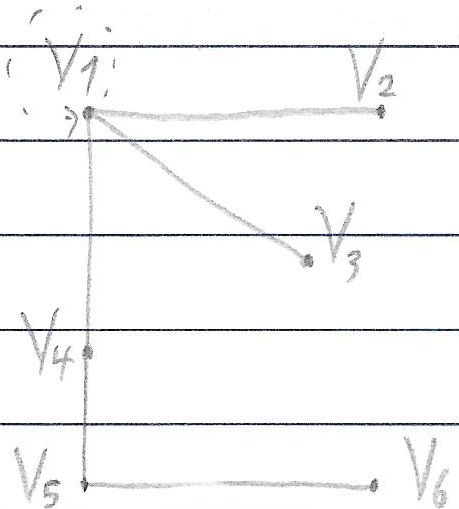
\includegraphics[scale=2]{graphG}
	\caption{Graph G}
	\label{fig:graphG}
	\end{figure}

	Vertex set: $\displaystyle V = \left\{ V_1, V_2, V_3, V_4, V_5, V_6 \right\}$ \linebreak 
	Edge set: $\displaystyle E= \left\{ \{V_1,V_2\}, \{V_1,V_3\}, \{V_1, V_4\}, \{V_4, V_5\}, \{V_5, V_6\} \right\}$ defines sets of edges, ie. vertices directly connecting each other. \linebreak 
	
	\textbullet \quad \uline{Cardinality} of a graph is the number of its vertices. eg. $|G| = 6$ \linebreak 
	\textbullet \quad \uline{Degree of }$\uline{V_1} = \deg (V_1) = 3$  :  The degree of a vertex, say $V_1$ (Graph G), is the number  of vertices it is directly connected with. \linebreak 
	\textbullet \quad The edges don't need to be straight, as long as the connections are preserved. Such graphs are called \uline{isomorphic}. For example, graphs G and G' are isomorphic. \linebreak 
	
	\begin{figure}[H]
	\centering
	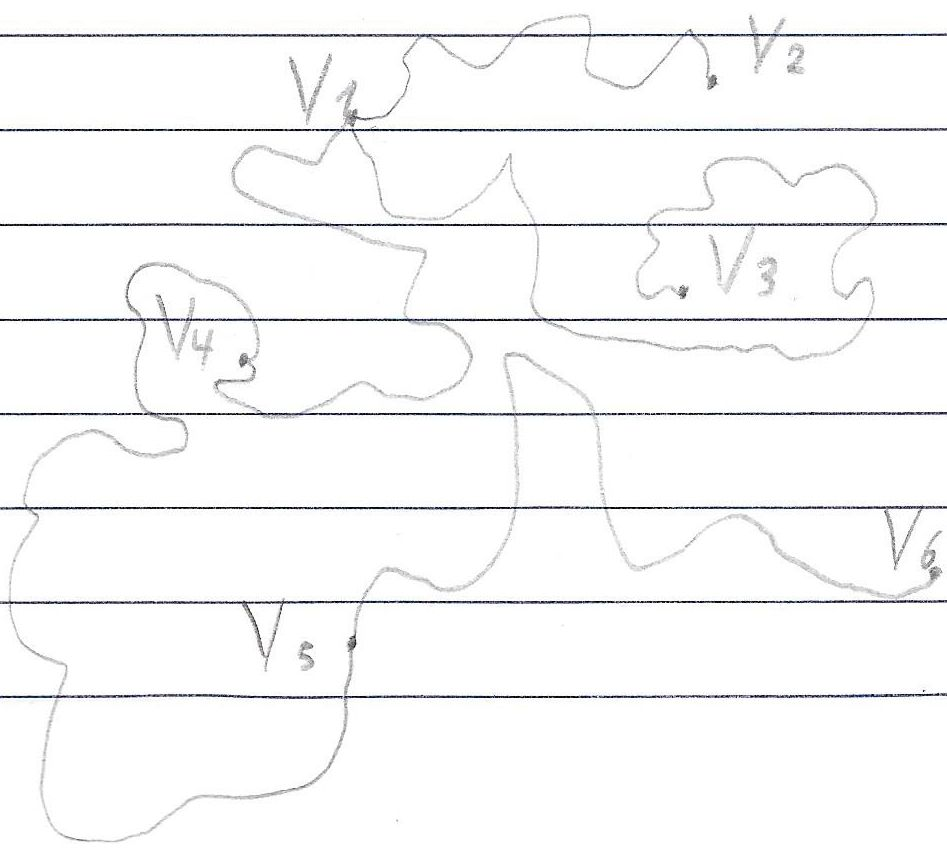
\includegraphics[scale=1]{graphG_}
	\caption{Graph G'}
	\label{fig:graphG_}
	\end{figure}
	
	\textbullet \quad \uline{Adjacency List}: We list vertices adjacent to each vertex. eg. For graph G, we have: \linebreak 
	$V_1: V_2, V_3, V_4$ \linebreak 
	$V_2: V_1$ \linebreak 
	$V_3: V_1$ \linebreak 
	$V_4: V_1, V_5$ \linebreak 
	$V_5: V_4, V_6$ \linebreak 
	$V_6: V_5$ \linebreak 
	
	\textbullet \quad \uline{Adjacency Matrix}: In every place of the matrix we insert a $1$, if there is a connection between the corresponding vertices, or a $0$ if there is not. For graph G, the adjacency matrix is the one pictured below (\figref{adjacencyMatricGraphG}) \linebreak 
	
	\begin{figure}[ht]
	\centering
	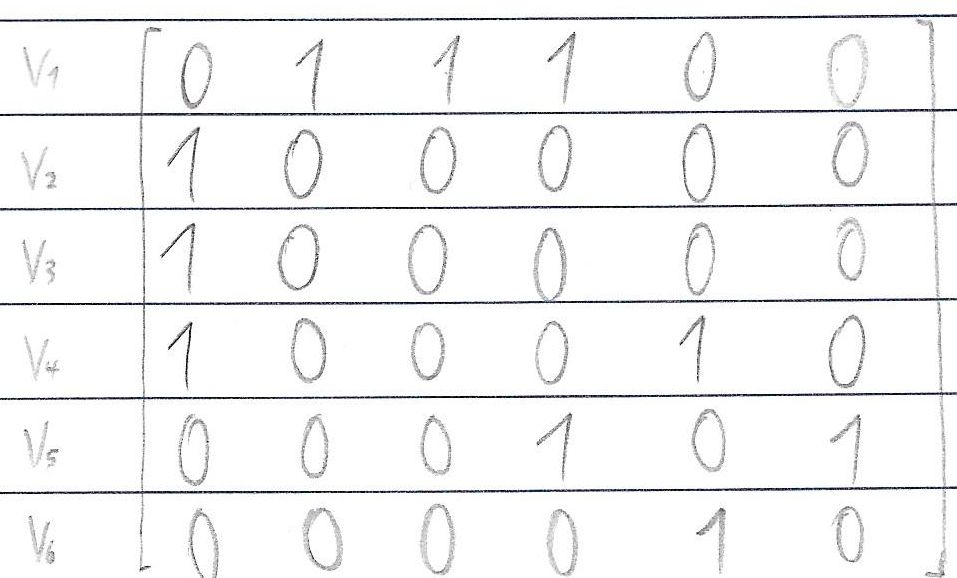
\includegraphics[scale=1]{adjacencyMatricGraphG}
	\caption{Adjacency Matric for the Graph G}
	\label{fig:adjacencyMatricGraphG}
	\end{figure}
	
	\textbullet \quad Graph C below (\figref{graphC}) is called a circuit, because there is at least one vertex, say D, from which we can start and without ever backtracking or lifting the pen, we can return back to it through a route, specified by the edges of the graph. Possible routes in this case are DABCD, DCBAD. \linebreak 
   
   	\begin{figure}[ht]
	\centering
	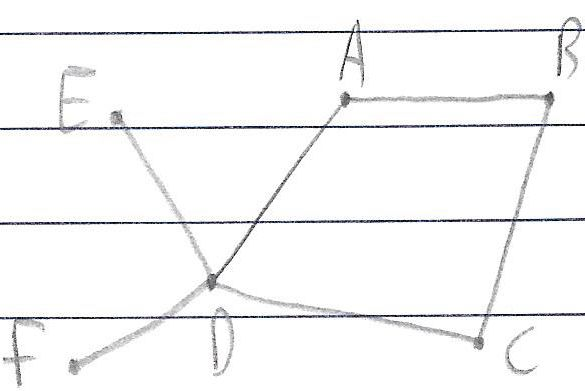
\includegraphics[scale=1]{graphC}
	\caption{Graph C - A circuit}
	\label{fig:graphC}
	\end{figure}
	
	\textbullet \quad A \uline{cyclic graph} is a graph containing at least one graph cycle. A graph that is not cyclic is said to be acyclic. A cyclic graph possessing exactly one (undirected, simple) cycle is called a unicyclic graph. Cyclic graphs are not trees. \linebreak 
	\textbullet \quad A \uline{tree} (\figref{graphGtree}) is an \uline{undirected graph} in which any two vertices are connected by exactly one path. In other words, any acyclic connected graph is a tree. \linebreak 
	\textbullet \quad A \uline{forest} is an undirected graph, all of whose connected components are trees; in other words, the graph consists of a disjoint union of trees. Equivalently, a forest is an undirected acyclic graph. \linebreak 
		
	\begin{figure}[ht]
	\centering
	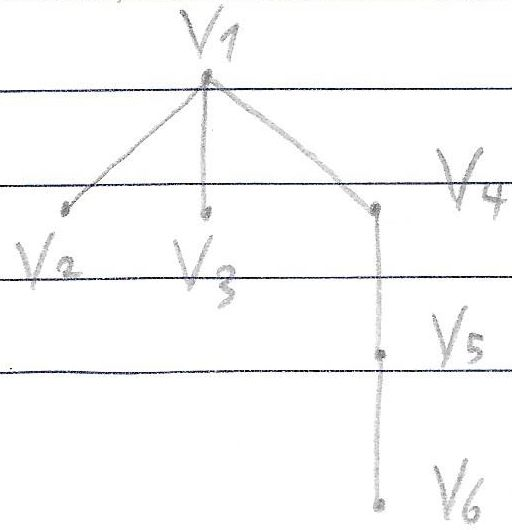
\includegraphics[scale=1]{graphGtree}
	\caption{Graph G is in fact a Tree}
	\label{fig:graphGtree}
	\end{figure}
	
	\textbullet \quad A Eulerian trail, or Eulerian path is a trail in a graph which visits every edge exactly once. \linebreak 
	\textbullet \quad A Eulerian circuit, or Eulerian cycle is an Eulerian trail which starts and ends on the same vertex. \linebreak 
		
	\textbullet \quad We have a graph $G = (V, E) $, where $V, E$ the sets of vertices and edges in the graph respectively. \linebreak 
	$\displaystyle \sum \limits_{v\in V} d(v) = 2|E| $, where $d(v)$ the grade of vertex $v$ \linebreak 

	
	\pagebreak
	
	
	\section{Discrete Math}
	
	\textbullet \quad Sigma notation definition: $\sum \limits_{i=a}^b f(i) \triangleq 
			\begin{cases} 
				0 &b < a \\
				f(a) + \sum \limits_{i=a+1}^b f(i) & b\geq a						
			\end{cases} $ \linebreak 
	\textbullet \quad Permutation of Indices: $\sum \limits_{n=1}^N b_{n+1} = \sum \limits_{n=2}^{N+1} b_n$ \linebreak 
	\textbullet \quad $\ceil{n/2} + \floor{n/2} = n \ \forall n \in \mathcal{Z} $ \linebreak 
	\textbullet \quad \uline{Pigeonhole Principle} (\textgreek{Αρχή του Περιστερώνα}): \textgreek{Με οποιονδήποτε τρόπο να τοποθετήσουμε} $n$ \textgreek{περιστέρια σε $m$ φωλιές, με $n > m$ θα υπάρχει τουλάχιστον μια φωλιά με} $ \ceil{n/m} $ \textgreek{περιστέρια}. \linebreak 
	\textbullet \quad \uline{Zero-based numbering}, or index origin = $0$, is a way of numbering in which the initial element of a sequence is assigned the index 0, rather than the index 1 as is typical in everyday non-programming context. Under zero-based numbering, the initial element is sometimes termed the zeroth element, rather than the first element; zeroth is a coined ordinal number corresponding to the number zero. \linebreak 
	\textbullet \quad $ e^x \geq 1 + x \ , \ \forall x \in \mathcal{R} $ \linebreak 
	\textbullet \quad $ \frac{x}{1+x} \leq \ln(1+x) \leq x \ , \ x > -1 $ \linebreak 
	
	\textbullet \quad Golden Ratio (\textgreek{Χρυσή Τομή}) \linebreak 
   Two quantities are in the golden ratio if their ratio is the same as the ratio of their sum divided by the larger of the two quantities. Some twentieth-century artists and architects, including Le Corbusier and Dalí, have proportioned their works to approximate the golden ratio—especially in the form of the golden rectangle, in which the ratio of the longer side to the shorter is the golden ratio—believing this proportion to be aesthetically pleasing. The golden ratio appears in some patterns in nature, including the spiral arrangement of leaves and plantlife. \linebreak 
   	$\displaystyle \phi \def \frac{a+b}{a} = \frac{a}{b}$ \linebreak 
	Its value is: $\displaystyle \phi = \frac{1+\sqrt{5}}{2} = 1.61803\ 39887 \in \mathcal{Q} $ \linebreak 
	\uline{Properties} \linebreak 
	\textbullet \quad $\displaystyle 1+\frac{1}{\phi} = \phi $ , which can be arranged into... \linebreak 
	\textbullet \quad $\displaystyle \phi +1=\phi ^2$ \linebreak 
	\textbullet \quad $\displaystyle \frac{1}{\phi} + \frac{1}{\phi^2} = 1$ \linebreak 
	\textbullet \quad Using the quadratic formula for the above, two solutions are obtained: \linebreak 
	$\displaystyle \phi =\frac {1+{\sqrt {5}}}{2}= 1.61803\ 39887 \ldots$ and $\displaystyle \overline{\phi} =\frac {1-{\sqrt {5}}}{2} = -0.61803\ 39887 \dots $ \linebreak 
	
		\subsection{Asymptotic Notations and Growth of Functions}
	
	\textbullet \quad \uline{Stirling's approximation}: $\displaystyle n! \approx \sqrt{2\pi n} \left(\frac{n}{e}\right)^n \Bigg(1 + \Theta \Big(\frac{1}{n}\Big) \Bigg) $ , for large $n$. \linebreak	
	\textbullet \quad $ n! \geq \Big( \frac{n}{3} \Big)^n $ \linebreak 	
	
	\textbullet \quad $\displaystyle \sum\limits_{i=1}^n \log(i) = \log (n!) \approx n \log (n) $, ie. $\displaystyle log(n!) = \Theta (n\log (n))$ \linebreak 
	\textbullet \quad $\displaystyle \lim \limits_{x\to \infty} \sqrt[x]{x} = 1$ \linebreak 
	\textbullet \quad If $\displaystyle \lim_{n\to \infty} \frac{T(n)}{g(n)} = 0 \rightarrow T(n) = o \left( g(n) \right) $ \linebreak 
	ie. $T(n)$ has a much smaller rate of growth to that of $g(n)$ as $n$ grows without measure $\forall n \geq n_0 $. \linebreak 
	\textbullet \quad If $\displaystyle \lim_{n\to \infty} \frac{T(n)}{g(n)} = c \ > 0 \rightarrow T(n) = \omega \left( g(n) \right) \ \land \ T(n) = o \left( g(n) \right) , \ \text{thus} \ T(n) = \Theta \left( g(n) \right) $ \linebreak 
	ie. $T(n)$ and $g(n)$ have the \uline{same} rates of growth. \linebreak 
	\textbullet \quad If $\displaystyle \lim_{n\to \infty} \frac{T(n)}{g(n)} = \pm \infty \rightarrow T(n) = \omega \left( g(n) \right) $ \linebreak 
	ie. $T(n)$ has a much greater rate of growth to that of $g(n)$ as $n$ grows without measure $\forall n \geq n_0 $. \linebreak 	
	
	\subsection{Sequences and Series}
	
	\textbullet \quad \uline{Arithmetic Series} is a sequence (/series) of numbers in which each differs from the preceding one by a constant quantity. \linebreak 
	\textbullet \quad $u_n = \alpha + (n-1) d$  :  General term \linebreak 
	\textbullet \quad $\displaystyle \sum \limits_{r=0}^{n-1} (a+rd) = \frac{n}{2}\left[2a+(n-1)d \right] $  :  Sum \linebreak 
	or $S_n = \displaystyle \sum \limits_{r=1}^n \left(a+rd\right) = n \frac{(a_1+a_n)}{2}\ , \ a_1 $ is first term \& $a_n$ is the last term. \linebreak 
	\textbullet \quad $b = \frac{a + c}{2} , a < b < c$  :  Arithmetic mean \linebreak 
	
	\textbullet \quad \uline{Geometric Series} is a series with a constant ratio between successive terms. \linebreak 
	\textbullet \quad $u_n = a\cdot r^{n-1} $  :  General term \linebreak 
	\textbullet \quad $\displaystyle \sum \limits_{k=0}^{n-1} ar^k = a\frac{(1-r^n)}{1-r}$, or more generally .. \linebreak 
	\textbullet \quad $\displaystyle \sum \limits_{k=m}^n r^k = \frac{a(r^m-r^{n+1})}{1-r} $ \linebreak 
	\textbullet \quad $\displaystyle |r| < 1 \longrightarrow \sum \limits_{k=0}^\infty ar^k = \frac{a}{1-r} $ \linebreak 
	\textbullet \quad $ b=\sqrt{ac} \quad, a<b<c$  :  Geometric mean \linebreak 
	
	\textbullet \quad \uline{Harmonic Series} is the series: $\displaystyle  \sum \limits_{n=1}^{\infty} \frac{1}{n} = 1 + \frac{1}{2} + \frac{1}{3} + \frac{1}{4} + \frac{1}{5} + \ldots = \log (n) + \mathcal{O}(1) $ \linebreak 
	\textbullet \quad $\displaystyle u_n = \frac{1}{n} , n\in \mathbb{N}^* $  :  General term \linebreak 
	\textbullet \quad $\displaystyle b=\frac{2ac}{a+c} = \frac{2}{\frac{1}{a} + \frac{1}{c}}, a< b<c $  :  Harmonic mean \linebreak 
	\textbullet \quad $ H_k = \sum\limits_{i=1}^k = 1 + \frac{1}{2} + \frac{1}{3} + \frac{1}{4} + \ldots + \frac{1}{k} $  :  Harmonic number \linebreak 
	\textbullet \quad $ H_{2^n} \leq 1 + n $ \linebreak 
	\textbullet \quad $ \frac{x}{x - 1} \leq 2 \ , \ \forall x \geq 2 $ \linebreak 
	\textbullet \quad The sum of the first $n$ terms of the harmonic series is given analytically by the $n$th harmonic number: \linebreak 
	$\displaystyle H_n = \sum \limits_{k=1}^n \frac{1}{k} = \gamma + \psi_0 (n+1) $ \linebreak 
	where $\gamma$ is the Euler-Mascheroni constant and $\psi_0(\chi)$ is the digamma function. \linebreak 
	
	\textbullet \quad \uline{Euler's number}: $e$ is a mathematical constant that is the base of the natural logarithm: the unique number whose natural logarithm is equal to one. The number $e\approx 2.71828$ is the limit of $\displaystyle \left( 1 + \frac{1}{n} \right)^n$ as $n$ approaches infinity, an expression that arises in the study of compound interest. It can also be calculated as the sum of the infinite series: \linebreak 
	$\displaystyle e= \sum \limits_{n=0}^{\infty} \frac{1}{n!} = \frac{1}{1} + \frac{1}{1} + \frac{1}{1\cdot 2} + \frac{1}{1\cdot 2 \cdot 3} + \cdots $ \linebreak 
	The constant can be characterized in many different ways. For example, $e$ can be defined as the unique positive number a such that the graph of the function $y = a^x$ has unit slope at $x = 0$. The function $f(x) = e^x$ is called the (natural) exponential function. The natural logarithm, or logarithm to base $e$, is the inverse function to the natural exponential function. The natural logarithm of a positive number $k$ can be defined directly as the area under the curve $y = 1/x$ between $x = 1$ and $x = k$, in which case $e$ is the value of $k$ for which this area equals one (see \figref{exponentialNumberAreaCurve}). \linebreak 
	
	\pagebreak
	
	\begin{figure}[H]
	\centering
	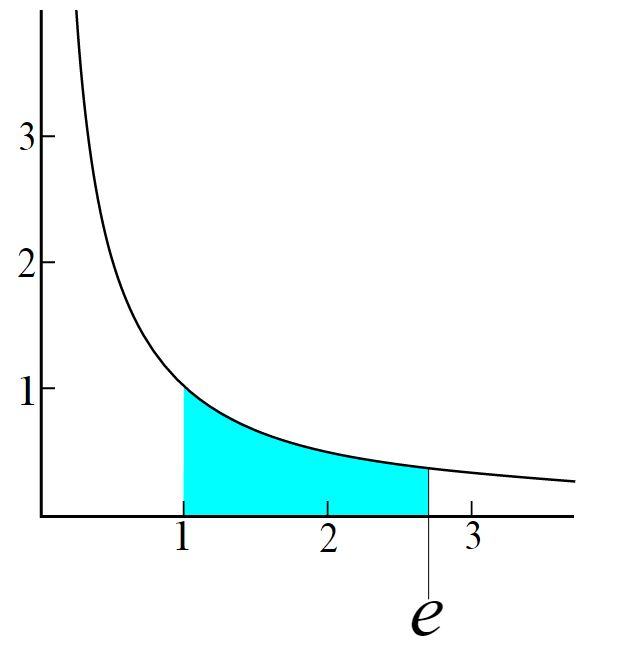
\includegraphics[scale=0.4]{exponentialNumberAreaCurve}
	\caption{$e$ is the unique number that makes the shaded area under the curve $y = 1/x$ equal to 1}
	\label{fig:exponentialNumberAreaCurve}
	\end{figure} 
	
	\uline{Sum of the Powers of Natural Numbers} \linebreak 
	\textbullet \quad $\displaystyle \sum \limits_{r=1}^n r = \frac{n(n+1)}{2} $ \linebreak 
	\textbullet \quad $\displaystyle \sum \limits_{r=k}^m r = k \cdot (m - k + 1) + \sum \limits_{i=1}^{m-k} i $ \linebreak 
	\textbullet \quad $\displaystyle \sum \limits_{r=1}^n r^2 = \frac{n(n+1)(2n+1)}{6} $ \linebreak 
	\textbullet \quad $\displaystyle \sum \limits_{r=1}^n r^3 = \left\{ \frac{n(n+1)}{2} \right\}^2 $ \linebreak 
	\textbullet \quad $\displaystyle \sum \limits_{k=0}^\infty x^k= \frac{1}{1-x}, |x| < 1 $ \linebreak 
	\textbullet \quad $\displaystyle \sum \limits_{k=0}^\infty kx^k= \frac{x}{(1-x)^2}, |x| < 1 $ \linebreak 
	\textbullet \quad $\displaystyle \sum \limits_{i=m}^n c = c \cdot (n - m + 1) $ \linebreak 
	\textbullet \quad $\displaystyle \sum \limits_{i=m}^n i = \frac{(n-m+1)(n+m)}{2} $ \linebreak 
	
	\uline{Infinite Series}: $\displaystyle \sum \limits_{k=1}^{\infty} u_k = u_1 +u_2 +u_3 + \ldots + u_n + \ldots $ \linebreak 
	\textbullet \quad  $\lim_{n\to\infty} \sum \limits_{k=1}^{\infty} u_k $ is a definite value $\rightarrow$ Series is convergent \linebreak 
	\textbullet \quad $ \lim_{n\to\infty} \sum \limits_{k=1}^{\infty} u_k $ is not a definite value $\rightarrow$ Series is divergent \linebreak 
	
	Relationship between Summation and Product notations: \linebreak 
	$\displaystyle \prod \limits_{r=\text{sth}}^{n \text{or} \infty} k^r = k^{\sum \limits_{r=\text{sth}}^{n \text{or} \infty}} r$ \linebreak 
	$\displaystyle \sum \limits_{k=1}^n \log k = \log \bigg( \prod \limits_{k=1}^n k \bigg) = \log (n!) $ \linebreak 
	
	\uline{Decimal Representation}: A decimal representation of a non-negative real number $r$ is an expression in the form of a series, traditionally written as a sum: $\displaystyle r = \sum \limits_{i=0}^{\infty} \frac{a_i}{10^i} $, where $a_0$ is a nonnegative integer, and $a_1, a_2, \ldots$ are integers satisfying $0\leq a_i \leq 9$ called the digits of the decimal representation. The sequence of digits specified may be finite, in which case any further digits $a_i$ are assumed to be 0. \linebreak 
	The number defined by a decimal representation is often written more briefly as \\
	$\displaystyle r=a_{0}.a_{1}a_{2}a_{3}\dots .\ $ \linebreak 
	That is to say, $a_0$ is the integer part of $r$, not necessarily between $0$ and $9$, and $a1, a2, a3, \ldots $ are the digits forming the fractional part of $r$. \linebreak 
	\textbullet \quad A sequence is called monotone if it is either increasing, or decreasing. \linebreak 
	
	\uline{Tests for Convergence}  
	\begin{enumerate}
	\item $\lim_{n\to\infty} u_n = 0 \rightarrow $ series may be convergent, \\ 
			$\lim_{n\to\infty} u_n \neq 0 \rightarrow $ series is certainly divergent \linebreak 
			
	\item Comparison test - Useful standard series \\ 
		\textbullet \quad $\displaystyle \frac{1}{1^p} + \frac{1}{2^p} + \frac{1}{3^p} + \frac{1}{4^p} + \ldots + \frac{1}{n^p} + \ldots $  :  P-series \linebreak 
			For $p>1$ series converges. For $p\leq 1$, series diverges \linebreak 
		\textbullet \quad $1 - \frac{1}{2} + \frac{1}{3} - \frac{1}{4} + \frac{1}{5} - \ldots $ \linebreak 
		
	\item D'Alembert's ratio test for positive terms \linebreak 
		\textbullet \quad $\lim_{n\to\infty} \left| \frac{u_{n+1}}{u_n} \right| < 1 \longrightarrow $ limit converges \linebreak 
		\textbullet \quad $\lim_{n\to\infty} \left| \frac{u_{n+1}}{u_n} \right| > 1 \longrightarrow $ limit diverges \linebreak 
		\textbullet \quad $\lim_{n\to\infty} \left| \frac{u_{n+1}}{u_n} \right| = 1 \longrightarrow $ inconclusive assessment \linebreak 
		
	\item For General Series \linebreak 
		\textbullet \quad $\sigma |u_n| $ converges $ \longrightarrow \sigma u_n $ is absolutely convergent \linebreak 
		\textbullet \quad $\sigma |u_n| $ diverges $ \land \ \sigma u_n $ converges $\longrightarrow \sigma u_n $ is conditionally convergent \linebreak 
		
	\item Limit Comparison Test \linebreak 
	\textbullet \quad Suppose $b_n$  :  known series, $a_n$  :  series under test \linebreak 
	$0 < \lim_{n\to\infty} \frac{a_n}{b_n} < \infty \longrightarrow $ both series behave in like manners \linebreak 	 
	 
	\item Monotone Convergence Theorem \linebreak 
	\textbullet \quad Lemma 1: If a sequence of $ \mathbb{R}$ is increasing and bounded above, then its supremum is the limit. The supremum is defined as the least upper bound of a sequence / function. \linebreak 
	\textbullet \quad Lemma 2: If a sequence of real numers is decreasing and bounded below, then its infimum is the limit. \linebreak 
	\textbullet \quad Theorem: If $\{a_n\} $ is a monotone sequence of real numbers (i.e. if $a_n \leq a_{n+1}$, for every $n\geq 1$, or $a_n \geq a_{n+1}$, for every $n\geq 1$) then this sequence has a finite limit if and only if the sequence is bounded (a sequence is called "bounded", when it's bounded above and below). \linebreak 
	
	\item \uline{Alternating sign test}: Based on the alternating harmonic series: $\frac{(-1)^{n+1}}{n}$ If the magnitude of the terms decreases and the signs alternate then the series converges.  
	\end{enumerate}
	
	\textbullet \quad \uline{Taylor Series}: $\displaystyle f(x_0 + h) = f(x_0) + hf'(x) + \frac{h^2}{2!}f''(x) + \frac{h^3}{3!}f'''(x) + \ldots $ \\ 
		where $f(x)$ is continuous in $Dom(f)$. \linebreak 
	\textbullet \quad \uline{McLaurin Series}: $\displaystyle f(x) = f(0) + xf'(0) + \frac{x^2}{2!} f''(0) + \frac{x^3}{3!} f'''(0) + \ldots $ \\ 
		where $f(x)$ continuous in $Dom(f)$. McLaurin series describes the function $f(x)$ in terms of its successive derivatives at $x=0$ \linebreak 
	Useful / Common Series Expansions \linebreak 
	Reminder: In every trigonometric expansion the angle must be in radians \linebreak 
	\textbullet \quad $\displaystyle \sin (x) = x - \frac{x^3}{3!} + \frac{x^5}{5!} - \frac{x^7}{7!} + \frac{x^9}{9!} - \ldots $ \linebreak 
	\textbullet \quad $\displaystyle \cos (x) = 1 - \frac{x^2}{2!} + \frac{x^4}{4!} - \frac{x^6}{6!} + \frac{x^8}{8!} - \ldots $ \linebreak 
	\textbullet \quad $\displaystyle \sinh (x) = x + \frac{x^3}{3!} + \frac{x^5}{5!} + \frac{x^7}{7!} + \ldots $ \linebreak 
	\textbullet \quad $\displaystyle \cosh (x) = 1 + \frac{x^2}{2!} + \frac{x^4}{4!} + \frac{x^6}{6!} + \ldots $ \linebreak 
	\textbullet \quad $\displaystyle \tan (x) = x + \frac{x^3}{3} + \frac{2x^5}{15} + \frac{17x^7}{315} + \frac{62x^9}{2 835} + \ldots $ \linebreak 
	\textbullet \quad $\displaystyle \ln (1 \pm x) = \pm x -\frac{x^2}{2} \pm \frac{x^3}{3} -\frac{x^4}{4} \pm \frac{x^5}{5} - \ldots $ \linebreak 
	\textbullet \quad $\displaystyle e^x = 1 + x + \frac{x^2}{2!} + \frac{x^3}{3!} + \frac{x^4}{4!} + \ldots $ \linebreak 
	\textbullet \quad $\displaystyle e^{-x} = 1 - x + \frac{x^2}{2!} - \frac{x^3}{3!} + \frac{x^4}{4!} - \ldots $ \linebreak 
	\textbullet \quad Binomial Series: $\displaystyle  (1 \pm x)^n = 1 \pm nx + \frac{x^2}{2!}n(n-1) \pm \frac{x^3}{3!} n(n-1)(n-2) + \ldots $ \linebreak 
	\textbullet \quad  Binomial Expansion (General Case): $\displaystyle  (a+b)^n = ^{n}C_0 a^n b^0 + ^{n}C_1 a^{n-1} b^1 + ^{n}C_2 a^{n-2}b^2 + ^{n}C_3 a^{n-1}b^3 + \ldots + ^{n}C_n a^0 b^n $ \linebreak 
	\textbullet \quad $\displaystyle (1 \pm x)^{-1} = 1 \mp x + x^2 \mp x^3 + x^4 \mp \ldots $  :  Converges iff $|x| < 1$ \linebreak 
	\textbullet \quad $\displaystyle \frac{d}{dx}(1-x)^{-1} = \frac{1}{(1-x)^2} = 1 +2x + 3x^2 +4x^3 +5x^4 +\ldots $ \linebreak 
	\textbullet \quad $\displaystyle \cos ^2(x) = x^2 -\frac{x^4}{3} + \frac{2x^6}{45} - \ldots $ \linebreak 
	\textbullet \quad $\displaystyle \sin ^{-1}(x) = x + \frac{x^3}{3} + \frac{3x^5}{40} + \ldots $ \linebreak 
	\textbullet \quad $\displaystyle e^{ax} = 1 + ax + \frac{x^2x^2}{2!} + \frac{a^3x^3}{3!} + \frac{a^4x^4}{4!} + \ldots $ \linebreak 
	\textbullet \quad $\displaystyle \tan^{-1}(x) = x -\frac{x^3}{3} + \frac{x^5}{5} -\frac{x^7}{7} + \frac{x^9}{9} -\ldots $ \linebreak 
	\textbullet \quad $\displaystyle e = \lim_{n\to\infty} \left(1 + \frac{1}{n} \right)^n = \lim_{n\to 0} \left(1 + n \right)^\frac{1}{n} $ \linebreak 
	
		\textbullet \quad Harmonic numbers are the numbers $H_n$ for $n\geq 1$ defined by $H_n = \sum \limits_{i=1}^n \frac{1}{i}$ \\ $\forall n,m \in \mathbb{N} \left(n\geq m \rightarrow H_n -H_m \geq \frac{n-m}{n} \right) \quad \sum \limits_{k=1}^{n-1} H_k = nH_n -n $ \linebreak 
	\textbullet \quad $ 2^n -1 = 1 + 2 + 2^2 +2^3 +\ldots + 2^{n-1} = \sum \limits_{k=0}^{n-1} 2^k $ \linebreak 
	\textbullet \quad $ 2^n -2^{n-1} = 2^{n-1} $ \linebreak 
	\textbullet \quad $\displaystyle  1 + 3 + 3^2 +3^3 + \ldots + 3^n = \frac{3^{n+1}-1}{2} $ \linebreak 
	\textbullet \quad The \uline{length} of $[1+2+3+\ldots +2^n +(2^n+1) +(2^n+2) +(2^n+3)+\ldots +2^{n+1} ], n\geq 1 $, is a power of $2$. \linebreak 
	\textbullet \quad $\sum \limits_{i=1}^n i(i!) = (n+1)! - 1$ \linebreak 
	
	\uline{Fibonacci Sequence} \linebreak 	
	\textbullet \quad The definition is given by the recurrence relation: $\displaystyle F_{n} = F_{n-1} + F_{n-2}$ \linebreak 
	where $\displaystyle  F_0 = 0, F_1 = 1 $ or $\displaystyle F_1 = F_2 = 1$ \linebreak 
	\textbullet \quad $\displaystyle F_n = F_{n-1} + F_{n-2} = \frac{(\frac{1+\sqrt{5}}{2})^n-(\frac{1-\sqrt{5}}{2})^n}{\sqrt{5}}	$ \linebreak 
	\textbullet \quad $\sum \limits_{i=0}^n F_{2i} = F_0 + F_2 + F_4 +\ldots+F_{2n} = F_{2n+1} -1$ \linebreak 
	
	\textbullet \quad The sequence $a_0, a_1, a_2, \ldots$ is called a generalized Fibonacci sequence, or a Gibonacci sequence, if \\ $\forall n \geq 2(a_n = a_{n-2} + a_{n-1} )$. \\
	Also, $\displaystyle \exists s,t \in \mathbb{R} \left[ a_n = s\left(\frac{1+\sqrt{5}}{2} \right)^2 + t\left( \frac{1-\sqrt{5}}{2} \right)^2 \right] $ \linebreak 
	
	\textbullet \quad The Lucas numbers are the numbers $L_0, L_1, L_2, \ldots $ defines as follows: $\displaystyle a) L_0 = 2, \quad	 b) L_1 = 1, \quad \forall n \geq 2 L_n = L_{n-2} + L_{n-1} = \left(\frac{1+\sqrt{5}}{2}\right)^n + \left(\frac{1-\sqrt{5}}{2}\right)^n $ \linebreak 

	\textbullet \quad Triangular numbers: $T_n = \sum \limits_{k=1}^n k = \frac{n(n+1)}{2} $  :  equal to the number of dots composinga triangle with $n$ dots on one side \linebreak 
	\textbullet \quad $T_n + T_{n-1} = n^2 = (T_n - T{n-1})^2 $ \linebreak 
	
	\textbullet \quad \uline{Dirichlet series}: is any series of the form: \linebreak 
	$\displaystyle \sum\limits_{n=1}^{\infty} \frac{a_n}{n^s} $ \linebreak 
	where $s \in \mathcal{C} \ $ and $a$ is a complex sequence. The Dirichlet series plays a varierty of important roles in analytic number theory (the branch of Mathematics connecting Number Theory / Discrete Math and Calculus). \linebreak 
	
	\textbullet \quad $\displaystyle \frac{\pi^2}{6} = \frac{1}{1^2} + \frac{1}{2^2} + \frac{1}{3^2} + \frac{1}{4^2} + \frac{1}{5^2} + \ldots $ \linebreak 
	
	\textbullet \quad Mersenne sequence: $ f(x) = 2^n - \ , \ n \in \mathbb{N} $ \linebreak 
	
	\subsection{Fourier Series}
	
	\textbullet \quad Approximates the values of a periodic function: $ f(x+T) = f(x)$, where $T$ is the period. \linebreak 
	\textbullet \quad The Fourier series converges to $f(x)$, if the Dirichlet conditions are satisfied (sufficient conditions).  
	\begin{enumerate}
	\item The function $f(t)$ must be defines single valued \& periodic. 
	\item $f(t)$ and $f'(t)$ have at most a finite number of finite discontinuities over a single period - i.e. they are piecewise continuous. 
	\end{enumerate}
	\textbullet \quad $f(t) = \frac{a_0}{2} + \sum \limits_{n=1}^{\infty} \left(a_n \cos (n\omega t) + b_n \sin (n\omega t) \right) $, $a_0, a_n, b_n$ are the Fourier coefficients \linebreak 
	$a_0 = \frac{2}{T} \int_{-T/2}^{T/2} f(t) dt $ \linebreak 
	$a_n = \frac{2}{T} \int_{-T/2}^{T/2} f(t) \cos (n\omega t) dt \ , \qquad 	b_n = \frac{2}{T} \int_{-T/2}^{T/2} f(t) \sin (n \omega t) dt $ \linebreak 
	\textbullet \quad Alternative notation for real valued function $f(t)$ with complex coefficients: $f(t) = \sum \limits_{n=-\infty, n\neq 0}^{\infty} c_n e^{jn\omega t} \quad where c_n = \frac{1}{T} \int_{-T/2}^{T/2} f(t) e^{-jn \omega_0 t} dt = \frac{a_n -j b_n}{2} = |c_n| e^{j\phi n} $  :  Discrete complex spectrum \linebreak 
	
	\begin{figure}[ht]
	\centering
	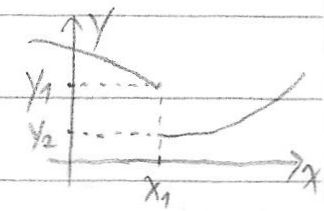
\includegraphics[scale=2]{finiteDiscontinuity}
	\caption{Sum of Fourier series at a finite discontinuity}
	\label{fig:finiteDiscontinuity}
	\end{figure}	
	
	\textbullet \quad Sum of Fourier series at a finite discontinuity: At $x = x_1$ series for $f(x)$ converges to the value: $ 1/2 (f(x_{1-}) + f(x_{1+}) ) = 1/2 (y_1 + y_2) $ \linebreak 
	\textbullet \quad  Alternative notation: $f(t) = \frac{a_0}{2} + \sum \limits_{n=1}^{\infty} c_n \sin (n\omega t + \phi_n) $ \\ 
		$c_n = \sqrt{a_n^2 + b_n^2}\ , \quad \phi_n = \tan^{-1} (\frac{a_n}{b_n}) $ \linebreak 
	\textbullet \quad The constant (D.C.) term $a_0/2$ is to raise, or lower the entire waveform on the y-axis. \linebreak 
	
	\begin{figure}[p]
	\centering
	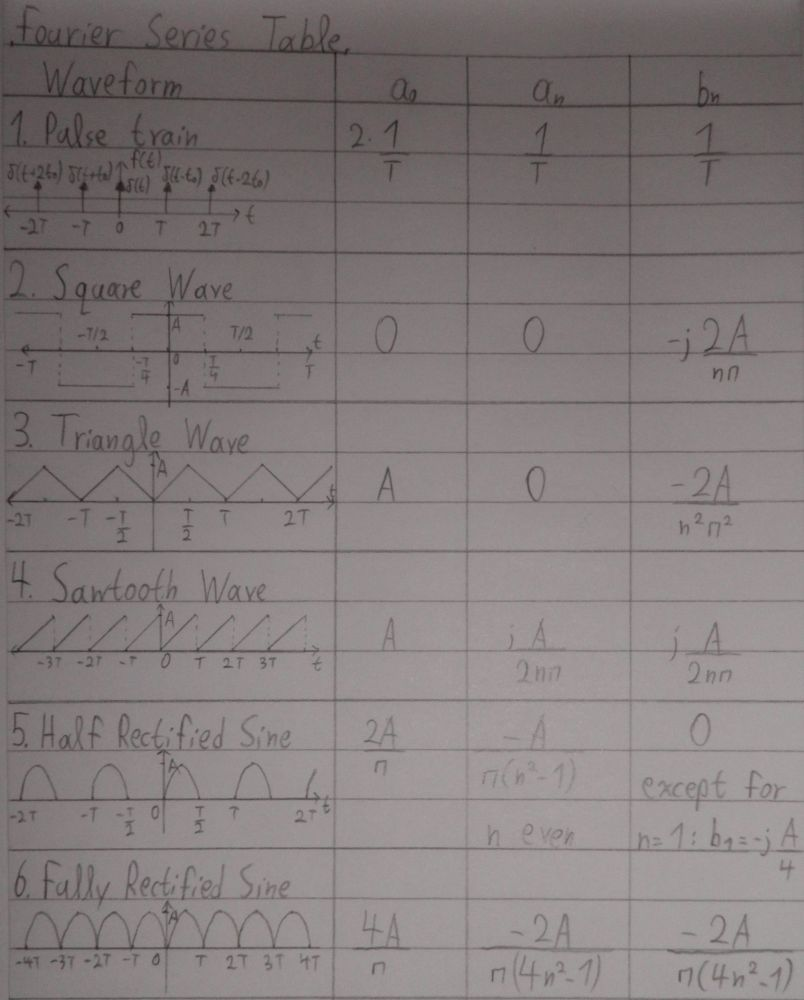
\includegraphics[scale=0.55]{fourierSeriesTable}
	\caption{Fourier Series Table}
	\label{fig:fourierSeriesTable}
	\end{figure}
	
	
	\pagebreak
	
	
	\section{Probability Theory}
	
	\textbullet \quad \textgreek{Αν σε} $\nu$ \textgreek{εκτελέσεις ενός πειράματος ένα ενδεχόμενο} $A$ \textgreek{πραγματοποιείται} $k$ \textgreek{φορές, τότε ο λόγος} $\frac{k}{\nu}$ \textgreek{ονομάζεται σχετική συχνότητα του} $A$ \textgreek{και συμβολίζεται με} $f_A$. \linebreak 
	\textbullet \quad \textgreek{\uline{Στατιστική ομαλότητα ή Νόμος των Μεγάλων Αριθμών}}: \textgreek{Οι σχετικές συχνότητες πραγματοποίησης ενός πειράματος, που εκτελείται κάτω από αμετάβλητες συνθήκες, σταθεροποιούνται γύρω από κάποιους αριθμούς (όχι πάντοτε ίδιους), καθώς ο αριθμός των δοκιμών του πειράματος επαναλαμβάνεται απεριόριστα}. \linebreak 
	
	\uline{\textgreek{Αξιωματική Θεμελίωση Πιθανότητας}} \linebreak 
	\textgreek{Έστω} $\displaystyle \Omega= \{ \omega_1, \omega_2, \ldots , \omega_{\nu} \} $ \textgreek{δειγματικός χώρος με πεπερασμένο πλήθος στοιχείων. Ισχύουν τα παρακάτω}: \linebreak 
	\textbullet \quad $\displaystyle 0 \leq P(\omega_i) \leq 1 \quad , 1\leq i \leq \nu $ \linebreak 
	\textbullet \quad $\displaystyle P(\Omega ) = P(\omega_1) + P(\omega_2) + \ldots + P(\omega_{\nu} ) = 1$ \linebreak 
	\textbullet \quad \textgreek{Εάν} $\displaystyle \omega_1, \omega_2, \ldots, \omega_{\nu}$ \textgreek{είναι ανά δύο ασυμβίβαστα, δηλαδή} $\displaystyle \omega_i \cap \omega_j = \emptyset$, \textgreek{τότε}: $\displaystyle P(\omega_1 + \omega_2 + \ldots + \omega_{\nu}) = P(\omega_1) + P(\omega_2) + \ldots + P(\omega_{\nu}) $ \linebreak 
	\textbullet \quad $\displaystyle P(\emptyset) = 0$ \linebreak 
	\textbullet \quad \textgreek{Αν} $\displaystyle P(\omega_i) = \frac{1}{\nu}$ \textgreek{, τότε έχουμε τον κλασικό ορισμό της πιθανότητας ενός ενδεχομένου (ισοπίθανα ενδεχόμενα)}: \linebreak 
	$$ P(A) = \frac{\text{\textgreek{Πλήθος Ευνοϊκών Περιπτώσεων}}}{\text{\textgreek{Πλήθος Δυνατών Περιπτώσεων}}} = \frac{N(A)}{N(\Omega)}$$ 
	\textbullet \quad $\displaystyle P(A \cup B) = P(A + B) $ (alternative notation) \linebreak 
	\textbullet \quad $\displaystyle P(A \cap B) = P(A \cdot B) $ (alternative notation) \linebreak 
	\textbullet \quad $\displaystyle P(A') = 1 - P(A) $ \linebreak 
	\textbullet \quad $\displaystyle P(A \cup B) = P(A) + P(B) - P(A \cap B) $ (additive law) \linebreak 
	\textbullet \quad $\displaystyle A\cap B = \emptyset \rightarrow P(A\cup B) = P(A) + P(B)$ (simple additive law) \linebreak 
	\textbullet \quad $\displaystyle A \subset B \rightarrow P(A) \leq P(B) $ \linebreak 
	\textbullet \quad $\displaystyle P(A-B) = P(A) -P(A\cap B) = P(A \cap B') $ \linebreak 
	\textbullet \quad $\displaystyle \forall A,B \in \Omega \ P(B) = P(B\cdot A + B \cdot A') $ \linebreak 

	\begin{figure}[H]
	\centering
	
\includegraphics[scale=2]{pithanotita1}
	\caption{\textgreek{Διάγραμμα} Venn \textgreek{της πιθανότητας: } $P(A-B) + P(B-A)$}
	\label{fig:pithanotita1}
	\end{figure}
	
	\textbullet \quad $\displaystyle P(A-B) + P(B-A) = P(A \cdot B') + P(B\cdot A') $ \figref{pithanotita1} \linebreak 
	\textbullet \quad $\displaystyle P(A|B) = \frac{P(A\cap B)}{P(B)}\ , \ P(B) > 0 $ \textgreek{(δεσμευμένη πιθανότητα)} \linebreak 	
	\textbullet \quad $\displaystyle P(A\cap B) = P(A|B) \cdot P(B) = P(B|A) \cdot P(A) $ \textgreek{(πολλαπλασιαστικός νόμος των πιθανοτήτων)} \linebreak 
	\textbullet \quad $\displaystyle P(A|B) = \frac{P(B|A) \cdot P(A)}{P(B)} $ \textgreek{: θεώρημα } Bayes, \textgreek{επίσης}: \linebreak 
	$ P(A|B) = \frac{P(A)\ P(B|A)}{P(A)\ P(B|A) + P(\overline{A})\ P(B|\overline{A})} $ \linebreak 
	\textbullet \quad \textgreek{Δύο ενδεχόμενα} $A$ \textgreek{και} $B$ \textgreek{με} $P(A) > 0 $ \textgreek{και} $P(B) > 0$ \textgreek{λέγονται} \uline{\textgreek{ανεξάρτητα}}, \textgreek{αν και μόνον αν} $P(A \cap B) = P(A) \cdot P(B) $ \linebreak 
	\textbullet \quad $A,B$ \textgreek{ανεξάρτητα ενδεχόμενα} $\rightarrow P(A|B) = P(A)$ \textgreek{και} $P(B|A) = P(B)$ \linebreak 
	\textbullet \quad $P(A) = P(A \cap B_1) + P(A \cap B_2) + \ldots + P(A \cap B_{\nu}) = \sum \limits_{i=1}^{\nu} P(A|B_i) \cdot P(B_i) $ \textgreek{μόνον αν} $B_1, B_2, \ldots, B_{\nu} $ \textgreek{ασυμβιβαστά ενδεχόμενα και } $B_1 + B_2 + \ldots + B_{\nu} = \Omega $ \linebreak 
	\textbullet \quad $P(A+B+ \Gamma) = P(A) + P(B) + P(\Gamma) - P(AB) - P(A\Gamma) - P(B\Gamma) + P(AB\Gamma) $ \linebreak 
	\textbullet \quad $ \sum \limits_{i=1}^{\nu} P(x_i | y) = 1$ \linebreak 
	\textbullet \quad An experiment that has a \uline{result} with more than one possible \uline{outcomes} is referred to as a \uline{random experiment}. The only requirement that is made of the outcomes of a random experiment is that they be mutually exclusive. To cater for ranges of possible outcomes we define an \uline{event}. An event consists of one or more outcomes selected from a list of all possible outcomes. \linebreak 
	
	\textbullet \quad \uline{Indicator function} is a function that returns the value of 1 when something is true and 0 when it is false. \linebreak 
	\textbullet \quad \uline{Indicator Random variable} has value 1 if something is going to happen and 0 otherwise. 
	$$ \mathbf{1}[A] = \left\{\begin{array}{cc} 1, & \notin \mathcal{A} \\ 0, & x \in \mathcal{A} \end{array}\right.$$ 
	For $N$ trials the probability of $1$'s will be $N \cdot \mathbf{1}[A]$ and the long term average value for these $N$ trials will be $P(N)$. \linebreak 
	\textbullet \quad \uline{Expected value} of a discrete random variable is $R$ defined as following. Suppose $R$ can take value $r_1$ with probability $p_1$, value $r_2$ with probability $p_2$, and so on, up to value $r_k$ with probability $p_k$. Then the expectation of this random variable $R$ is defined as \linebreak 
	$$ E[R] = r_1 \cdot p_1 + r_2 \cdot p_2 + \ldots + r_k \cdot p_k $$
	\textbullet \quad \uline{Linearity of Expectation}: Let $R$, $S$ be random variables of some probability space and $a$, $b$ constants. Then the following holds: \linebreak 
	$$ E\{a\cdot R + b \cdot S\} = a \cdot E\{R\} + b \cdot E\{S\} $$
	\textbullet \quad \uline{Central Limit Theorem}: Given certain conditions, the arithmetic mean of a sufficiently large number of iterations of independent random variables, each with a well defined (finite) expected value and finite variance, will be approximately normally distributed, regardless of the underlying normal distribution. \linebreak  \textgreek{Αναλυτικότερα: Δίνονται οι Τ.Μ.} $X_i$ \textgreek{και} $X = X_1 + X_2 + \ldots + X_n$ \textgreek{το άθροισμα τους. Το άθροισμα αυτό αποτελεί μια Τ.Μ. με μέση τιμή}: $m = m_1 + m_2 + \ldots + m_n$ \textgreek{και διακύμανση} $\sigma^2 = \sigma_1^2 + \sigma_2^2 + \ldots + \sigma_n^2 $. \textgreek{Το Κ.Ο.Θ. δηλώνει ότι, κάτω από ορισμένες γενικές συνθήκες, η κατανομή} $f_X(\chi)$ \textgreek{της} $X$ \textgreek{προσεγγίζει την κανονική κατανομή με την ίδια μέση τιμή} $m$ \textgreek{και διακύμανση} $\sigma^2: f(\chi) \simeq G\left( \frac{\chi -m}{\sigma} \right) $ \textgreek{καθώς το } $m$ \textgreek{αυξάνει ( θεωρητικά καθώς} $m \to \infty$). \linebreak 
	
	\textbullet \quad \uline{Law of large numbers (LLN)}: describes the result of performing the same experiment a large number of times. According to the law, the average of the results obtained from a large number of trials should be close to the expected value and will tend to become close as more trials are performed. \linebreak 
	
	\subsection{Combinatorics}
	
	\textbullet \quad \uline{\textgreek{Βασική Αρχή Απαρίθμησης (κανόνας γινομένου)}}: \textgreek{Έστω ότι μια διαδικασία μπορεί να πραγματοποιηθεί σε} $\nu$ \textgreek{διαδοχικές φάσεις} $\phi_1, \phi_2, \ldots, \phi_{\nu}$. \textgreek{Αν η φάση} $\phi_1$ \textgreek{μπορεί να πραγματοποιηθεί με} $k_1$ \textgreek{τρόπους και για καθέναν από αυτούς η φάση} $\phi_2$ \textgreek{μπορεί να πραγματοποιηθεί με} $k_2$ \textgreek{τρόπους, ... και για καθέναν από όλους αυτούς τους τρόπους η φάση} $\phi_{\nu}$ \textgreek{μπορεί να πραγματοποιηθεί με} $k_{\nu}$ \textgreek{τρόπους, τότε η διαδικασία αυτή μπορεί να πραγματοποιηθεί με} $k_1 \cdot k_2 \cdot \ldots \cdot k_{\nu} $ \textgreek{τρόπους.} \linebreak 
		\textbullet \quad \uline{\textgreek{Μεταθέσεις} (permutations)}: \textgreek{Στην περίπτωση που πάρουμε και τα } $\nu$ \textgreek{στοιχεία ενός συνόλου και τα βάλουμε σε μια σειρά, τότε έχουμε μια διάταξη των} $\nu$ \textgreek{στοιχείων ανά} $\nu$, \textgreek{η οποία λέγεται μετάθεση των} $\nu$ \textgreek{στοιχείων. Το πλήθος των μεταθέσεων θα είναι}: $M_{\nu}^{\nu} = M_{\nu} - \nu ! $ \linebreak 
	\textbullet \quad \uline{\textgreek{Διατάξεις} (k-permutations)}: \textgreek{Διάταξη των} $\nu$ \textgreek{στοιχείων ενός συνόλου ανά} $k$, \textgreek{με} $k\leq \nu$, \textgreek{λέγεται καθένας από τους διαφορετικούς τρόπους με τους οποίους μπορούμε να πάρουμε} $k$ \textgreek{διαφορετικά στοιχεία του συνόλου και να τα βάλουμε σε μια σειρά. (διατάξεις των }$\nu$ \textgreek{ανά} $k$  : ) $\displaystyle \Delta_k^{\nu} = \nu (\nu -1) (\nu-2) \ldots(\nu -k + 1) = \frac{\nu!}{(\nu-k)!} $ \linebreak 
	Notes: \linebreak 
	- The order of elements matters. \linebreak 
	- No elements may appear more than once. \linebreak 
	\textbullet \quad \uline{\textgreek{Συνδυασμοί} (combinations)}: \textgreek{Συνδυασμός των} $\nu$ \textgreek{στοιχείων ενός συνόλου ανά} $k$ \textgreek{ονομάζεται κάθε υποσύνολο του συνόλου με} $k$ \textgreek{στοιχεία}. \linebreak 
	("$n$ choose $k$") $\displaystyle ^nC_k = \binom{n}{k} = \frac{n!}{k!(n-k)!}\ , \ n\geq k $ \linebreak 
	Notes: \linebreak 
	- Order doesn't matter. \linebreak 
	\textbullet \quad All combinations of sizes of the input sequence (eg. the Power set of the input set): \linebreak 
	$2^n$ \linebreak 
	
	\textbullet \quad \uline{Newton's Binomial}: \linebreak 
	$(a+b)^n = \sum \limits_{k=0}^{\infty} \binom{n}{k} a^{n-k} b^k \ , \ n\in \mathbb{N} \ \land a,b \in \mathbb{R}$ \linebreak 
	Properties: \linebreak 
	\textbullet \quad $\displaystyle \binom{n+1}{k} = \binom{n}{k} + \binom{n}{k-1} $, \textgreek{ή} $\binom{n}{k} = \binom{n-1}{k} + \binom{n-1}{k-1} $ \linebreak 
	\textbullet \quad $\displaystyle \binom{n}{0} + \binom{n}{1} + \binom{n}{2} + \ldots + \binom{n}{n} = 2^n $ \textgreek{ή} $ \sum \limits_{k=0}^{n} \binom{n}{k} = 2^n $ \linebreak 
	\textbullet \quad $\displaystyle \binom{n}{1} + \binom{n}{3} + \binom{n}{5} + \ldots = \binom{n}{0} + \binom{n}{2} + \binom{n}{4} + \ldots = 2^{n-1} $ \linebreak 
	\textbullet \quad $\displaystyle \binom{n}{0} ^2 + \binom{n}{1} ^2 + \binom{n}{2} ^2 + \ldots + \binom{n}{n} ^2 = \binom{2n}{n} $ \linebreak 
	
	\uline{Random Variables - (\textgreek{Τυχαίες Μεταβλητές})} \linebreak 
	A (discrete) random variable $X$ is a function from a finite, or countably infinite sample space $S$ to the real numbers. It associates a real number with each possible outcome of an experiment, which allows us to work with the probability distribution induced on the resulting set of numbers. \linebreak 
	\textbullet \quad $P(X \geq x) = 1 - P(X \leq x) $ \linebreak 
	\textbullet \quad $P(X \lesseqqgtr x) = P(X \lessgtr x) + P(X = x) $ \linebreak 
	\textbullet \quad $F_X (x) = P(X \leq x)\ , \ \forall x \in (-\infty , \infty) \ , \ $ $F_X$  :  \uline{\textgreek{Α.Σ.Κ}} \textgreek{της τ.μ. Χ.} \linebreak 
	\textbullet \quad \textgreek{Η} $F_X$ \textgreek{είναι μη φθίνουσα. Αν} $x_1 < x_2$, \textgreek{τότε} $F_X(x_1) \leq F_X(x_2)$ \linebreak 
	\textbullet \quad $F(+ \infty) = 1 \ , \ F(-\infty) = 0$ \linebreak 
	\textbullet \quad $\lim_{x\to \infty} F(X \leq x) = 1 \ , \ \lim_{x \to -\infty} F(X \leq x) = 0 $ \linebreak 
	\textbullet \quad $\forall x \leq x_0 (F_X (x_0) = 0 \rightarrow F_X (x) = 0 ) $ \linebreak 
	\textbullet \quad $0 \leq F(X \leq x) \leq 1\ , \ \forall x $ \linebreak 
	\textbullet \quad $F_X (-x) = F_X (x) $ \linebreak 
	\textbullet \quad $F_X$  :  \textgreek{συνεχής από τα δεξιά}: $F_X(x) = F_X(x^+)$ \linebreak 
	\textbullet \quad $P(x_1 < X < x_2) = F_X(x_2) - F_X(x_1)$ \linebreak 
	\textbullet \quad $P(X = x) = F_X(x) -F_X(x^-) $ \linebreak 
	\textbullet \quad $P(x_1 \leq X \leq x_2) = F_X (x_2) - F_X(x_1^-)$ \linebreak 
	\textbullet \quad \textgreek{\uline{Σ.Π.Π.}}: $\displaystyle f_X(x) \overset{\triangle}{=} \frac{dF_X(x)}{dx} $ \textgreek{και} $\displaystyle F_X(x) \overset{\triangle}{=} \int_{-\infty}{x} f_X (u) du $ \linebreak 
	\textbullet \quad $P(X \in B)$, $B$  :  \textgreek{διάστημα} $ = \ \int_B f_X(x) dx$ \linebreak 
	\textbullet \quad $P(X=B) = f_X(B) $ \linebreak 
	\textbullet \quad $\int_{-\infty}^{\infty} f_X(x) dx = 1\ , \ \sum \limits_{x\in A} f_X(x) = 1 \ , \ \int_{-\infty}^{\infty} F_X(x) dx = 1$ \linebreak 
	\textbullet \quad $P(a\leq X \leq b) = \int_a^b f_X(x) dx$ \linebreak 
	
	\uline{Expected/Mean Value} \linebreak 
	\textbullet \quad $E(X) = \int_{-\infty}^{\infty} x f_X (x) dx $  :  for P.D.F. \linebreak 
	\textbullet \quad $E(X) = \sum \limits_i x_i P(x_i) $  :  for P.M.F. \linebreak 
	Properties: \linebreak 
	\textbullet \quad $E(C) = C$  :  \textgreek{σταθερά} \linebreak 
	\textbullet \quad $E(C\cdot X) = C \cdot E(X) $ \linebreak 
	\textbullet \quad $E(C\cdot X + b) = C \cdot E(X) + b$ \linebreak 
	
	\uline{Variance} \linebreak 
	\textbullet \quad $\sigma_X^2 = E(X^2) - \left[ E(X)^2 \right] $  :  Variance \linebreak 
	Properties: \linebreak 
	\textbullet \quad $\Var(C) = 0 $ \linebreak 
	\textbullet \quad $\Var(C\cdot X) = C^2 \cdot \Var(X) $ \linebreak 
	\textbullet \quad $\Var(C\cdot X + b) = C^2 \cdot \Var(X) $ \linebreak 
	
	\textbullet \quad \uline{Covariance} (\textgreek{συνδιασκύμανση}) of two r.v.: A measure of how much two r.v. change together. \linebreak 
	$\displaystyle \Cov(X,Y) = E\big[(X-E[X]) \cdot (Y-E[Y]) \big] = E[X\cdot Y] - E[X] \cdot E[Y] $ \linebreak 
	
	\textbullet \quad Error probability: $P_e = P(e | X=x_1) \cdot P(X= x_1) + P(e|X=x_0) \cdot P(X \approx x_2) + \ldots + P(e|X = x_n) \cdot P(X=x_n) $ \linebreak 
	\textbullet \quad Q function , $X$ is gaussian r.v. \linebreak 
	\textbullet \quad $Q(X) = 1 - F_X(x) \ , \ Q(-x) = 1 - Q(x) \ , \ Q(x) $  :  \textgreek{φθίνουσα} \linebreak 

	\subsection{Probability Distributions}
	
	\uline{Bernoulli trials}: A Bernoulli trial is any random experiment (r.e.) whose result has only two outcomes, which we shall call success with probability $p$ and failure with probability $q$ . $P(\text{success}) = p$, $P(\text{failure}) = q$. Thus $p+q=1$. \linebreak 
	
	\uline{Binomial \textgreek{(Διωνυμική)} Distribution}: gives the discrete probability distribution $P(n|N)$ of obtaining exactly $n$ successes out of $N$ Bernoulli trials. \linebreak 
	$\displaystyle P(n|N) = \binom{N}{n} p^n q^{N-n} = \frac{N!}{n!(N-n)!} p^n (1-p)^{N-n} \ , \ $ where $\binom{N}{n}$ is the binomial coefficient. \linebreak 
	
	\uline{Geometric Distribution}: is the D.P.D. of the number $X$ of Bernoulli trials needed to get one success \linebreak 
	$P(X=k) = pq^{k-1}\ $, $k$ trials ($k\in \mathbb{N}$), $X$  :  number of attempts until the first success \linebreak 
	Properties: 
	\begin{itemize}
	\item (i) \quad $E[X] = \frac{1}{p}$, 
	\item (ii) \quad $\Var[X] = \frac{(1-p)}{p^2}$ 
	\item (iii) \quad The Expected value / Mean of a D.R.V. following the geometric distribution is the inverse of its parameter. eg. $\displaystyle X_i = \text{Geo}(\frac{6-i}{6}) \rightarrow E[X_i] = \frac{6}{6-i}$ 
	\end{itemize}
	It is the discrete analog of the exponential distribution. \linebreak 
	
	\uline{Poisson Distribution}: is a D.P.D. that expressses the probability of a given number of events $k$ occuring in a fixed interval of values (e.g. time), if these events occur with a known average rate $\lambda$ (rate parameter) and independently of the time since the last event. \linebreak 
	$P(k$ events in interval$) = P(X=k) = e^{-\lambda} \frac{\lambda^k}{k!} $  :  P.M.F. , $ k\in \mathbb{N} $ \linebreak 
	$\lambda$  :  average number of events per interval. \linebreak 
	Properties:  
	\begin{itemize}
	\item (i) \quad $E[X] = \lambda$, 
	\item (ii) \quad $\Var[X] = \lambda$  
	\end{itemize}

	\uline{Exponential Distribution}: is the P.D. that describes the time between events in a \uline{Poisson process} (i.e. a process in which events occur continuously and independently at a constant average rate) \linebreak 
	$f_X(x) = \begin{cases} \lambda e^{-\lambda x} \ , &\ x\geq 0 \\ 0 \ , &\ otherwise \end{cases} $ \linebreak 
	$\lambda$  :  rate parameter (slope of curve) \linebreak 
	Properties:
	\begin{itemize}
	\item (i) \quad $E[X] = \frac{1}{\lambda} $, 
	\item (ii) \quad $\Var[X] = \frac{1}{\lambda^2} $
	\end{itemize}
	
	\uline{Uniform Distribution}: is a family of symmetric P.D.'s such that for each member of the family, all intervals of the same length on the distribution's support are equal. \linebreak 
	$$ \text{C.D.F.}: F_X(x) 
	\begin{cases} 
		1 \ , & \ x \geq b \\ 
		\frac{x-a}{b-a} \ , & \ a\leq x \leq b \\ 
		0 \ , \ x<a	
	\end{cases} $$ 
	P.D.F.: \linebreak 
	$$\displaystyle f_X(x) = 
	\begin{cases} 
	\frac{1}{b-a} \ , & \ a\leq x \leq b \\ 
	0 \ , & \ otherwise	
	\end{cases}$$
	Properties: 
	\begin{itemize}
	\item (i) \quad $E[X] = \frac{a+b}{2} $, 
	\item (ii) \quad $\Var[X] = \frac{(b-a)^2}{12} $ 
	\end{itemize}
	If the random variable $X$ follows the uniform distribution we'll indicate that, by writing: $X \thicksim \cup (a,b) $ \linebreak 
	
	\uline{Normal Distribution}: A C.R.V. $X$ is a normal, or Gauss R.V. with parameters $\mu$ and $\sigma^2$ , if its P.D.F. is: \linebreak 
	$\displaystyle f_X (\chi) = \frac{1}{\sqrt{2\pi \sigma^2}} e^{-\frac{(\chi-\mu)^2}{2\sigma^2}} \quad , \ -\infty < x < \infty \quad , \ \sigma^2: $ variance, $\ \mu$  :  mean / expected value \linebreak 
	C.D.F.: $F_X(\chi) = \int_{-\infty}^x f_X^(y) dy \overset{\triangle}{=} G\big( \frac{\chi - \mu}{\sigma} \big) $\linebreak 
	The cumulative distribution function is often given tabulated ($G$). \linebreak 
	Standard Normal Distribution: P.D.F.: $\displaystyle y = \phi(z) = \frac{1}{\sqrt{2\pi}} e^{-\frac{z^2}{2}} \ $, where $z= \frac{\chi -\mu}{\sigma} $ \qquad $\mu = 0\ , \ \sigma = 1$ \linebreak 
	
	Area under the standard normal curve: $P(\alpha \leq z \leq b) $ \linebreak 
	$P($values within 1s.d. of the mean) $ = 68\%$ \linebreak 
	$P($values within 2s.d. of the mean) $ = 95\%$ \linebreak 
	$P($values within 3s.d. of the mean) $ =99.7\%$ \linebreak 
	
	\subsection{Stochastic Processes}
	
	\textbullet \quad A \uline{Markov} process, is a stochastic process that satisfies the Markov property (sometimes characterized as "memorylessness"). A process satisfies the Markov property if one can make predictions for the future of the process based solely on its present state just as well as one could knowing the process's full history, hence independently from such history. \linebreak 
	\textbullet \quad The Markov property refers to the memoryless property of a stochastic process.  \linebreak 
	\textbullet \quad Memorylessness is a property of certain probability distributions. It usually refers to the cases when the distribution of a "waiting time" until a certain event, does not depend on how much time has elapsed already. Only two kinds of distributions are memoryless: exponential distributions of non-negative real numbers and the geometric distributions of non-negative integers. \linebreak 
	
	
	\pagebreak
	
	
	\section{Statistics}
	
	\textbullet \quad $\displaystyle \nu_1 + \nu_2 + \nu_3 + \ldots + \nu_k = \nu$  :  \textgreek{Το άθροισμα των (απόλυτων) συχνοτήτων είναι ίσο με το μέγεθος του δείγματος} $\nu$. \linebreak 
	\textbullet \quad $\displaystyle f_i = \frac{\nu_i}{\nu} $  :  \textgreek{Σχετική συχνότητα} (relative frequency) \textgreek{της τιμής} $x_i \ 0\leq f_i \leq 1 \ $ , 	\textgreek{αφού} $\ 0 \leq \nu_i \leq \nu$ \linebreak 
	$\displaystyle f_i(\%) = 100\cdot f_i $ \linebreak 
	\textbullet \quad \textgreek{Το σύνολο των} $\left(x _{i}, \nu _{i} \right)$ \textgreek{αποτελεί την κατανομή συχνοτήτων} \linebreak 
	\textbullet \quad \textgreek{Το σύνολο των} $\left( x_i, f_i \right) $ \textgreek{ή} $(x_i, f_i(\%))$ \textgreek{αποτελεί την κατανομή σχετικών συχνοτήτων} \linebreak 
	\textbullet \quad \textgreek{Για τις ποσοτικές μεταβλητές εκτός από τα} $\nu_i, f_i $ \textgreek{χρησιμοποιούνται συνήθως και οι λεγόμενες αθροιστικές συχνότητες} (cumulative frequencies) $N_i$ \textgreek{και οι αθροιστικές σχετικές συχνότητες} (cumulative relative frequencies) $F_i$, \textgreek{οι οποίες εκφράζουν το πλήθος και το ποσοστό αντίστοιχα των παρατηρήσεων που είναι μικρότερες ή ίσες της τιμής} $x_i$. \linebreak 
	\textbullet \quad $\displaystyle \nu_k = N_k - N_{k-1} \ \land \ f_k = F_k - F_{k-1} $ \textgreek{(υποθέτοντας} $x_1 < x_2 < \ldots < x_k$ ) \linebreak 
	\textbullet \quad \textgreek{Η γωνία} $\phi_i$ \textgreek{που αντιστοιχεί στο αντίστοιχο κυκλικό διάγραμμα συχνοτήτων} (piechart) \textgreek{είναι} $\displaystyle \phi_i = \nu_i \frac{360^o}{\nu} = 260^o f_i \ $ , \textgreek{για} $i=1,2,\ldots , k$. \linebreak 
	\textbullet \quad \textgreek{Σε ιστόγραμμα / διάγραμμα με άνισο πλάτος} $w_i$ \textgreek{κλάσεων, το ύψος της κλάσης είναι}: $\displaystyle h_i = \frac{\nu_i}{w_i}$, \textgreek{ή} $\displaystyle h_i^* = \frac{f_i(\%)}{w_i} $ \linebreak 
	\textbullet \quad \textgreek{Σε ένα ιστόγραμμα συχνοτήτων το εμβαδόν του ορθογωνίου ισούται με τη συχνότητα της κλάσης αυτής}. \linebreak 
	\textbullet \quad \textgreek{Αν στα ιστογράμματα συχνοτήτων θεωρήσουμε δύο ακόμη υποθετικές κλάσεις, στην αρχή και στο τέλος, με συχνότητα μηδέν και στη συνέχεια ενώσουμε τα μέσα των άνω βάσεων των ορθογωνίων με ευθύγραμμα τμήματα, σχηματίζεται το} \uline{\textgreek{πολύγωνο συχνοτήτων} (frequency polygon)}. \textgreek{Το εμβαδό του χωρίου που ορίζεται από αυτό και τον οριζόντιο άξονα είναι ίσο με το άθροισμα των συχνοτήτων, δηλαδή με το μέγεθος του δείγματος ν, ή ίσο με 100 αν πρόκειται για ιστόγραμμα σχετικών συχνοτήτων}. \linebreak 
	
	\uline{\textgreek{Μέτρα θέσης} (Position Metrics)} \linebreak 
	\textbullet \quad $\displaystyle \overset{-}{x} = \frac{x_1 \nu_1 + x_2 \nu_2 + \ldots + x_k \nu_k}{\nu_1 + \nu_2 + \nu_3 +\ldots + \nu_k} = \frac{1}{\nu} \sum \limits_{i=1}^k x_i \nu_i = \sum \limits_{i=1}^k x_i f_i $  :  \textgreek{Αριθμητικός μέσος όρος} (Arithmetic mean) \linebreak
	\textgreek{όπου: } $x_1, x_2, \ldots, x_k $  :  \textgreek{οι τιμές της τ.μ. Χ με συχνότητες} $\nu_1, \nu_2, \ldots , \nu_k $ \textgreek{αντίστοιχα και } $f_i$ \textgreek{οι αντίστοιχες σχετικές συχνότητες}. \linebreak 
	\textbullet \quad $\displaystyle \overset{-}{x} = \frac{x_1 w_1 + x_2 w_2 + \ldots + x_{\nu} w_{\nu}}{w_1 + w_2 + w_3 +\ldots + w_{\nu}} = \frac{\sum \limits_{i=1}^{\nu}}{\sum \limits_{i=1}^{\nu} w_i} $  :  \textgreek{Σταθμισμένος μέσος όρος} (weighted mean) \linebreak 
	\textgreek{όπου} $x_1, x_2, \ldots, x_{\nu} $ \textgreek{οι τιμές, με συντελεστές βαρύτητας} $w_1, w_2, \ldots, w_{\nu}$. \linebreak 
	\textbullet \quad \textgreek{Η διάμεσος} (median) $\delta$ \textgreek{ενός πληθυσμού} $\nu$ \textgreek{παρατηρήσεων που έχουν διαταχθεί σε αύξουσα σειρά, είναι η μεσαία παρατήρηση όταν} $\nu$ \textgreek{περιττός, ή ο μέσος όρος (το ημιάθροισμα) των δύο μεσσαίων παρατηρήσεων όταν} $\nu$ \textgreek{άρτιος}. \linebreak 
	\textbullet \quad $P_k\ , \ k=1,2, \ldots , 99 $  :  \textgreek{Εκατοστημόρια} (percentiles) \linebreak 
	\textgreek{Οι τιμές} $P_1, P-2, \ldots , P_{99}$ \textgreek{χωρίζουν τη συνολική συχνότητα σε 100 ίσα μέρη. Δηλαδή, ορίζουμε ως κ-εκατοστημόριο, ή} $P_k$ \textgreek{την τιμή εκείνη για την οποία το πολύ} $k\%$ \textgreek{των παρατηρήσεων είναι μικρότερες του} $P_k$ \textgreek{και το πολύ} $(100-k)\%$ \textgreek{των παρατηρήσεων είναι μεγαλύτερες από την τιμή αυτήν. Ειδική περίπτωση εκατοστημορίων είναι τα} $\displaystyle P_{25}, P_{50} = \delta , P_{75} $ \textgreek{που λέγονται τεταρτημόρια. Αναφέρονται και ως} $Q_1, Q_2, Q_3$ \textgreek{αντίστοιχα.} \linebreak 
	\textbullet \quad \textgreek{Η επικρατούσα τιμή} $M_0$ \textgreek{, ή κορυφή} (mode) \textgreek{ορίζεται ως η παρατήρηση με τη μεγαλύτερη συχνότητα} $\nu_i$. \uline{\textgreek{Μπορεί να οριστεί και στην περίπτωση ποιοτικών δεδομένων}}, \textgreek{ενώ τα προηγούμενα μέτρα θέσης ορίζονται μόνο για ποσοτικά δεδομένα. Είναι δυνατό να υπάρχουν πολλαπλές, ή και καμιά επικρατούσα τιμή.} \linebreak 
	
	\uline{\textgreek{Μέτρα Διασποράς} (Dispersion Metrics)} \linebreak 
	\textbullet \quad \textgreek{Εύρος} (Range) $R$ = \textgreek{Μεγαλύτερη παρατήρηση} $-$ \textgreek{Μικρότερη παρατήρηση} \linebreak 
	\textbullet \quad $Q= Q_3 -Q_1$  :  \textgreek{Ενδοτεταρτημοριακό εύρος} (interquartile range) $\uparrow Q \Rightarrow \uparrow $ \textgreek{Διασπορά} \linebreak 
	\textbullet \quad Var$[X] = E\left[ (X - E[X] ) ^2 \right] = E\left[ X^2 \right] - (E\left[ X \right] )^2 = \sigma^2 $  :  \textgreek{Διακύμανση} \linebreak 
	$\displaystyle \sigma^2 = \frac{1}{\nu} \sum \limits_{i=1}^{\nu} (x_i\nu_i - \overset{-}{x} )^2 = \frac{1}{\nu} \sum \limits_{i=1}{\nu} (x_i \nu_i )^2 - \big( \frac{\sum \limits_{i=1}^{\nu} x_i \nu_i}{\nu} \big)^2 $  :  \textgreek{για μη ομαδοποιημένα δεδομένα} \linebreak 
	$\displaystyle \sigma^2 = \frac{1}{\nu} \sum \limits_{i=1}^k x_i^2 \nu_i - \big( \frac{\sum \limits_{i=1}^k x_i \nu_i}{\nu} \big)^2 $  :  \textgreek{για ομαδοποιημένα δεδομένα, εδώ} $x_i$ \textgreek{είναι οι κεντρικές τιμές της κάθε κλάσης} \linebreak 
	\textbullet \quad $\sigma = \sqrt{\sigma^2} $ \textgreek{: Τυπικής απόκλιση} (standard deviation) \linebreak 
	\textbullet \quad $\displaystyle CV = \frac{\sigma}{|\overset{-}{X}} \cdot 100(\%) $  :  \textgreek{Συντελεστής μεταβολής, ή σχετική τυπική απόκλιση} (Coefficient of variation, or relative standard deviation) \linebreak 
	$\downarrow CV \rightarrow $ \textgreek{Μεγαλύτερη ομοιογένεια στις τιμές} \linebreak 
	\textbullet \quad Mode of grouped data = $\displaystyle L + h \big( \frac{f_m-f_1}{2f_m-f_1-f_2} \big) $ \linebreak 
	$L$  :  lower boundary of modal class, $h$  :  size of modal class, $f_m$  :  frequency of modal class, $f_1$  :  frequency of class preceding the modal class, $f_2$  :  frequency of class proceeding modal class \linebreak 
	\textbullet \quad \uline{Pearson correlation coefficient $(r)$}: Gives the strength of a \uline{linear} relationship between the $n$ values of two variables $x_i$ and $y_i$. \linebreak  
	(Be aware that there may be correlation, but not linear one) \linebreak 
	$$ r= \frac{n\sum \limits_{i=1}^n x_i y_i - \left( \sum \limits_{i=1}^n x_i \right) \left( \sum \limits_{i=1}^n y_i \right)}{\sqrt{\left[ n\sum \limits_{i=1}^n x_i^2 - \left( \sum \limits_{i=1}^n x_i \right)^2 \right] \cdot \left[ n \sum \limits_{i=1}^n y_i^2 - \left( \sum \limits_{i=1}^n y_i \right)^2 \right]}} $$ 
	\textbullet \quad \uline{Spearman's rank correlation coefficient}: It doesn't measure the actual values, but rather the differences $(d_i)$ between the $n$ corresponding values of two categories (/columns of data): \linebreak 
	$\displaystyle r_s = 1 - \frac{6 \sum \limits_{i=1}^n d_i^2}{n(n^2-1)} $ \linebreak 
	
	
	\pagebreak
	
	
		
	\section{Number Theory}
	
	\textbullet \quad $\forall n, m \in \mathbb{Z} \left[ m\neq 0 \rightarrow \exists !q, r \in \mathbb{Z}\left(n = q\cdot m + r \land 0 \leq r < |m| \right) \right] $ \\ $q$ and $r$ are called quotient and remainder respectively, when $n$ is divided by $m$. \linebreak 
	\textbullet \quad $(n|m \land m>0) \rightarrow r \in \{0,1,2,\ldots,m-1\} $ \linebreak 
	\textbullet \quad $ r = 0 \rightarrow n=2q $  :  \textgreek{άρτιος} \linebreak 
	\textbullet \quad $ r = 1\rightarrow n = 2q + 1 $  :  \textgreek{περιττός} \linebreak 
	\textbullet \quad \uline{Well-Ordering principle}: Every nonempty set of $\mathbb{N}$ has a smallest element. \linebreak 
	\textbullet \quad $n$ is even iff $n^2$ is even. \linebreak 
	\textbullet \quad $\displaystyle \forall n \in \mathbb{N} \ \forall x \in \mathbb{R} \left[ n \ \text{is odd} \rightarrow (x+1)(x^n+1) \right] $ \linebreak 
	\textbullet \quad $n \in \mathbb{N} \rightarrow x^n -a^n = (x-a)(x^{n-1} + x^{n-2}a + x^{n-3}a^2 + \ldots +a^{n-1} )$ \linebreak 
	\textbullet \quad $\forall n \in \mathbb{N}^* \left[1 + 3 + 5 + 7 + \ldots + (2n -1) \right] = \nu^2 $ \linebreak 
	\textbullet \quad $\displaystyle \forall n \in \mathbb{N}^* \left[ 1\cdot 2 + 2 \cdot 3 + 3\cdot 4 + \ldots + n(n+1) = \frac{n(n+1)(n+2)}{3} \right] $ \linebreak 
	\textbullet \quad $\displaystyle \forall n \in \mathbb{N}^* \left(\frac{1}{2\cdot 2} + \frac{1}{2\cdot 3} + \frac{1}{3 \cdot 4} + \ldots + \frac{1}{n(n+1)} = \frac{n}{n+1} \right)$ \linebreak 
	\textbullet \quad $\displaystyle \forall n \in \mathbb{N}^* \forall x \in \mathbb{R} - \{1\} \left(1+x+x^2+\ldots  x^{n-1} = \frac{x^n-1}{x-1} \right) $ \linebreak 
	\textbullet \quad $ \forall n \in \mathbb{N}^* \geq 3 \left( n^2 > 2n + 1 \right) $ \linebreak 
	\textbullet \quad $\forall k, l \in \mathbb{Z} \left( k = 2l + 1 \rightarrow \exists m \in \mathbb{Z} \left(k^2 = 8m + 1 \right) \right) $ \linebreak 
	\textbullet \quad $\forall a \in \mathbb{Z} \left[ \left( a^2 = 3k \lor a^2 = 3k + 1 \right) \land k \in \mathbb{Z} \right] $ \linebreak 
	\textbullet \quad $ \forall n \in \mathbb{N} \geq 2 \left[ 1+2+2^2 + \ldots +2^{n-1}: \text{\textgreek{πρώτος}} \rightarrow 2^{n-1}(2^n-1): \text{\textgreek{τέλειος}} \right] $ \linebreak 
	\textbullet \quad A discrete logarithm is an interger $k$ solving the equation: $b^k = g$ where $b$ and $g$ are elements of a group, s.t. $k=\log_b g$ \linebreak 
	Discrete logarithms are the group theoretic analog of ordinary logarithms, which solve the same equation for $b$ and $g$ in the group of real numbers. \linebreak 
	\textbullet \quad A number $g$ is a \uline{primitive root} modulo $n$ if every number $a$ coprime to $n$ is congruent to a power of $g$ modulo $n$. That is, for every integer $a$ coprime to $n$, there is an integer $k$ such that $g\cdot k \equiv a \ (\mod \ n)$. Such $k$ is called the index or discrete logarithm of $a$ to the base $g\ \mod \ n$. \linebreak 
		
	
	\subsection{Division Properties}
	
	\textbullet \quad $ \forall a \in \mathbb{Z}^* \left(\pm 1|a \land \pm a|a \right) $ \linebreak 
	\textbullet \quad $ \forall b \in \mathbb{Z}^* (b|0) $ \linebreak 
	\textbullet \quad $ \forall a, b, c \in \mathbb{Z} \land b \neq 0 $ \textgreek{έχουμε}: 
	\qquad - $ a|b \land b|a \rightarrow a = b \lor a = -b $ \linebreak 
	\qquad - $ a|b \land b|c \rightarrow a|c $ \linebreak 
	\qquad - $ a|b \rightarrow \exists \lambda \in \mathbb{Z}(a|\lambda b) $ \linebreak 
	\qquad - $ a|b \land a|c \rightarrow a|(b+c) $ \textgreek{(Το αντίστροφο φυσικά δεν ισχύει)} \linebreak 
	\qquad - $ a|b \land b\neq 0 \rightarrow |a| \leq |b| $ \linebreak 
	\textbullet \quad $ \forall k, \lambda \in \mathbb{Z} \left[ (a|b \land a|c) \rightarrow a|(kb + \lambda c) \right] $ \\ 
		\qquad \textgreek{Το} $(kb+\lambda c) \in \mathbb{Z}$ \textgreek{λέγετεαι γραμμικός συνδυασμός των} $b, c$ \linebreak 
	
	\textbullet \quad $ \forall a, m \in \mathbb{Z} \left[ (m|a \land m>1 ) \rightarrow m\nmid(a+1) \right] $\linebreak 
	\textbullet \quad $\forall \alpha, \beta \in \mathbb{Z}$ \textgreek{Ο Μ.Κ.Δ. των α, β, όταν ένας τουλάχιστον από τους α, β είναι διάφορος του 0, είναι ο δ και είναι ο μεγαλύτερος από τους θετικούς κοινούς διαιρέτες τους. Δηλαδή, ο δ έχει τις ακόλουθες δύο ιδιότητες:} \\
	\qquad $\delta | \alpha \land \delta | \beta $ \linebreak 
	\qquad $(x|\alpha \land x|\beta ) \rightarrow x\leq \delta $ \linebreak 
	\textgreek{Λέμε ότι} $ \delta \gcd (a,b)$ \textgreek{, ή} $\delta = (a, b)$ \linebreak 
	\textbullet \quad \uline{\textgreek{Ευκλείδιος Αλγόριθμος}} \textgreek{Αν} $a, b \in \mathbb{N} $ \textgreek{και υ το υπόλοιπο της ευκλείδειας διαίρεσης του} $a$ \textgreek{με τον} $b$, \textgreek{τότε}: $\gcd (a,b) = \gcd (b,\upsilon) $ \linebreak 
	\textbullet \quad $\gcd (a,b) = \gcd (|a|, |b|) $ \linebreak 
	\textbullet \quad $(a,a) = a $ \linebreak 
	\textbullet \quad $(a,0) = a $ \linebreak 
	\textbullet \quad $(a,1) = 1 $ \linebreak 
	\textbullet \quad $\forall a, b \in \mathbb{N}^* \left(b|a \rightarrow (a,b) = b \right) $ \linebreak 
	\textbullet \quad $ \forall a,b,k \in \mathbb{N}, b\neq 0 \left((a,b) = (a-kb, b) \right) $ \linebreak 
	\textbullet \quad $\forall a, b, \in \mathbb{Z} \left( (a,b) = 1 \rightarrow a, b \right) $ \textgreek{πρώτοι μεταξύ τους} $)$ \linebreak 
	\textbullet \quad $ \forall a, b \in \mathbb{Z}, b \neq 0 \left[ \delta = \gcd(a,b) \rightarrow \delta = ka + lb \right] $  :  Bezout's Identity. \textgreek{Οι} k, l \textgreek{δεν είναι μοναδικοί.} \linebreak 
	\textbullet \quad $\forall a, b \in \mathbb{Z}, b\neq 0 \left(a,b \text{\textgreek{πρώτοι μεταξύ τους}} \leftrightarrow ka + lb = 1 \right) $ \linebreak 
	\textbullet \quad $\forall a, b \in \mathbb{Z}, b\neq 0 \left[ ka +lb = \delta \rightarrow \left(k(\frac{a}{\delta}) + l(\frac{b}{\delta}) = 1 \leftrightarrow (\frac{a}{\delta}, \frac{b}{\delta} = 1 \right) \right] $ \linebreak 
	\textbullet \quad $\forall a, b, c \in \mathbb{Z} \left((b,c) = 1 \land a|bc \rightarrow a|b \lor a|c \right) $ \linebreak 
	\textbullet \quad $ \forall a, b, c \in \mathbb{Z} \left( a|b\cdot c \land (a,b) = 1 \rightarrow a|c \right) $ \linebreak 
	\textbullet \quad $ \forall k, a, b \in \mathbb{Z} \left[ (ka, kb) = k(a, b) \right] $ \linebreak 
		\textgreek{Ανάλογες σχέσεις ισχύουν και για περισσότερους από δύο ακεραίους πχ.} $\left[ \delta = (a, b, c) \rightarrow \exists k, l, m \in \mathbb{Z} (\delta = ka + lb + mc) \right]$ \textgreek{και} $\left[ \delta = (\alpha, \beta, \gamma) \rightarrow (\alpha / \delta, \beta / \delta, \gamma / \delta) = 1 \right] $. \linebreak 
	\textbullet \quad $\delta = (a, b, c, \ldots) = ((a,b), c, d, \ldots) = (a, (b,c), d, \ldots) $ \linebreak 
	\textbullet \quad \textgreek{Ε.Κ.Π των} $a, b \in \mathbb{Z}^* $ \textgreek{είναι το μικρότερο από τα θετικά κοινά πολλαπλάσια των} $a, b$. \textgreek{Συμβολίζεται}: $\epsilon = lcm [a,b] $ \textgreek{ή} $\epsilon = [a,b]$ \textgreek{και} $\epsilon \in \mathbb{N}^*$ \textgreek{έχει τις ακόλουθες ιδιότητες}: \linebreak 
	\qquad $\epsilon = mul(a) \land \epsilon = mul(b) $ \linebreak 
	\qquad $[x= mul(a) \land x = mul(b) ] \rightarrow \epsilon \leq x $ \linebreak 
	\textbullet \quad $[a,b] = [|a|, |b|] $ \linebreak 
	\textbullet \quad $b|a \rightarrow [a, b] = a $ \linebreak 
	\textbullet \quad $ [a, 1] = a$ \linebreak 
	\textbullet \quad $ \forall a, b \in \mathbb{N}^* \left[ (a,b) \cdot [a,b] = a\cdot b\right] $ \linebreak 
	\textbullet \quad $ \forall a, b \in \mathbb{Z}^* \left[ (a, b) \cdot [a, b] = |a|\cdot |b| \right] $ \linebreak 
	\textbullet \quad \textgreek{Τα κοινά πολλαπλάσια δύο ακεραίων είναι πολλαπλάσια του ΕΚΠ τους} \linebreak 
	\textbullet \quad $\epsilon = [a, b, c, \ldots] = [[a,b], c, \ldots] = [a, [b, c], d, \ldots] $ \linebreak 
	\textbullet \quad \uline{\textgreek{Θεώρημα πρώτων αριθμών}}: \# \textgreek{Πρώτων μικρότερων του} $x \sim \frac{x}{\ln(x)} $ \\
		\textgreek{Πυκνότητα πρώτων αριθμών μέχρι τον} $x: x = \frac{1}{\ln(x)}$. \textgreek{Διατύπωση:} $\lim_{x\to\infty} \frac{\pi(x)}{x\log (x)} = 1 , \quad \pi(x): $ prime counting function (counts \# of primes under $ x \in \mathbb{Z}$ \linebreak 
		\textbullet $\frac{x}{\log (x)} $  :  approximates $\pi(x)$ as x increases without bound \linebreak 
	\textbullet \quad \textgreek{Κάθε ακέραιος} $p \neq 0, \pm 1$ \textgreek{λέγεται πρώτος, αν οι μόνοι θετικοί διαιρέτες του είναι οι} $1$ \textgreek{και} $|p|$. \linebreak 
	\textbullet \quad \textgreek{Κάθε θετικός ακέραιος μεγαλύτερος του 1έχει έναν τουλάχιστον πρώτο διαιρέτη} \linebreak 
	\textbullet \quad \textgreek{Αν α είναι ένας σύνθετος ακέραιος με} $a>1$, \textgreek{τότε υπάρχει ένας τουλάχιστον πρώτος αριθμός ρ, τέτοιος ώστε} $p|a$ \textgreek{και} $p \leq \sqrt{a}$.\linebreak 
	\textbullet \quad \textgreek{Αν ένας πρώτος ρ διαιρεί το γινόμενο οσωνδήποτε ακεραίων, τότε διαιρεί έναν τουλάχιστον, από τους ακεραίους αυτούς}. \linebreak 
	\textbullet \quad \textgreek{Κάθε τεικός ακέραιος α > 1 μπορεί να γραφεί κατά μοναδικό τρόπο στη μορφή: } $\alpha = p_1^{a_1} \cdot p_2^{a_2} \cdots p_k^{a_k} $ \textgreek{όπου οι} $p_1, p_2, \ldots, p_k$ \textgreek{είναι θετικοί πρώτοι με} $p_1 < p_2 < \ldots p_k$ \textgreek{και} $a_1, a_2, \ldots, a_k \in \mathbb{N}^*$. \textgreek{Τότε λέμε ότι το α είναι γραμμένος στην κανονική του μορφή}. \linebreak 
	\textbullet \quad \textgreek{Αν ο φυσικός αριθμός} $n$ \textgreek{δεν είναι τετράγωνο φυσικού τότε ο} $\sqrt{n}$ \textgreek{είναι άρρητος} \linebreak 
	\textbullet \quad \textgreek{Ο ευκλείδειος αλγόριθμος βασίζεται στο γεγονός ότι}: $\forall a, b, r \in \mathbb{N}, b\neq 0 (a>b \rightarrow a = qb + r \land b>r) $ \linebreak 
	\textbullet \quad $\forall a,b,c \in \mathbb{Z} (ax + by = c) $  :  \textgreek{Μια γραμμική διοφαντική εξίσωση και} $\delta = \gcd(a,b)$. \textgreek{Η εξίσωση έχει λύση ανν} $\delta | c$. \textgreek{Τότε υπάρχουν άπειρες λύσεις που δίνονται από τους τύπους} $x= x_0 +b\cdot n \land y =y_0 -a\cdot n), \forall n \in \mathbb{Z} $, \textgreek{όπου} $(x_0,y_0)$ \textgreek{μια λύση της γραμμικής διοφαντικής εξίσωσης}. \linebreak 
	\textbullet \quad $\forall a, b, k, l \in \mathbb{Z} \exists m \in \mathbb{N} \left[a = km + \upsilon \land b = lm + \upsilon \leftrightarrow a \equiv b (\mod m) \right]$ \linebreak 
	\textbullet \quad $ \forall a, b \in \mathbb{Z} \left[a\equiv b(\mod m) \leftrightarrow m|(a-b) \right] $ \linebreak 
	
	\uline{Congruent (\textgreek{ισουπόλοιποι}) Numbers} \linebreak 
	\textbullet \quad \textgreek{\uline{Ορισμός:} Έστω} $m$ \textgreek{θετικός ακέραιος. Δύο ακέραιοι} $a$ \textgreek{και} $b$ \textgreek{λέγονται ισουπόλοιποι με μέτρο} $m$, \textgreek{όταν διαιρούμενοι με} $m$ \textgreek{αφήνουν το ίδιο υπόλοιπο}. \linebreak 
	
	\textbullet \quad $a \equiv b (\mod m) \Leftrightarrow m | (a-b) $ \linebreak 
	\textbullet \quad $a \equiv a (\mod m) $ \textgreek{(ανακλαστική)} \linebreak 
	\textbullet \quad $a \equiv b (\mod m) \rightarrow b\equiv a (\mod m) $ \textgreek{(συμμετρική)} \linebreak 
	\textbullet \quad $\big[ a\equiv b (\mod m) \land b\equiv c (\mod m) \big]  \rightarrow a \equiv c (\mod m) $ (\textgreek{μεταβατική}) \linebreak 
	\textbullet \quad $ a \equiv b (\mod m) \land c \equiv d (\mod m) \begin{cases} 
		a + c \equiv b + d (\mod m) \\ 
		a - c \equiv b - d (\mod m) \\ 
		a \cdot c \equiv b \cdot d (\mod m) 
	\end{cases} $ \linebreak 
	\textbullet \quad $ \forall a, b, c \in \mathbb{Z} \left[ \exists m \in \mathbb{N} (a \equiv b (\mod m) ) \rightarrow a^n \equiv b^n (\mod m) \land n\in \mathbb{N} \right] $ \linebreak 
	\textbullet \quad \textgreek{Έστω} $ \delta = \gcd (a, m)$. \textgreek{Τότε} $ax \equiv b (\mod m)$ \textgreek{έχει μια λύση, ανν} $\delta | b$. \linebreak 
	\textbullet \quad \textgreek{Αν υ το υπόλοιπο της ευκλείδειας διαίρεσης του} $a\in \mathbb{Z}$ \textgreek{με τον} $m \in \mathbb{N}^*$, \textgreek{τότε} $a \equiv \upsilon (\mod m) $ \linebreak 
	\textbullet \quad $\forall m \in \mathbb{Z} \left[ m | b \rightarrow b \equiv 0 (\mod m) \right] $ \linebreak 
	\textbullet \quad $\forall m \in \mathbb{Z} \left[ m\equiv 0 (\mod m) \right] $ \linebreak 
	\textbullet \quad $\forall a \in \mathbb{Z} \left[ a^2 \equiv 0 (\mod 8) \lor a^2 \equiv 1 (\mod 8) \lor a^2 \equiv 4 (\mod 8) \right] $ \linebreak 
	\textbullet \quad $ \forall a, b \in \mathbb{Z} (a, b) = 5 \rightarrow \left( \frac{a}{\delta}, \frac{b}{\delta} \right) = 1$ \linebreak 
		\textgreek{Χρήσιμος μετασχηματισμός}: $\displaystyle A = \frac{a}{\delta} \rightarrow a = A \delta \land B = \frac{b}{\delta} \rightarrow b = B \delta $ \linebreak 
	\textbullet \quad $ \forall k \in \mathbb{Z} \left[ n = 2k + 1 \rightarrow 9^n + 1 \equiv 0 (\mod 10) \right] $ \linebreak 
	
	\textbullet \quad Euler / Euler-Mascheroni constant: \\ 
		$\displaystyle \gamma = \lim_{n\to\infty} \left(\sum \limits_{k=1}^n \frac{1}{k} - \ln(n) \right) = \int_{1}^{\infty} \left(\frac{1}{\lfloor x \rfloor} - \frac{1}{x} \right) dx \simeq 0.57 721 56649 \ldots \quad \lfloor x \rfloor $  :  floor function \linebreak 
	\textbullet \quad The positive integers $i$ and $j$ are called \uline{relatively prime}, or \uline{coprime} if they share no common factors. In other words $i$ and $j$ are coprime if their only common factor is $1$. \linebreak 
	\textbullet \quad \uline{Mersenne prime}: $ M_n = 2^n -1 \ , \quad n \in \mathbb{N} $ \linebreak 
	\textbullet \quad If $2^p -1$ is prime then $2^{p-1} (2^p -1) $ is a \uline{perfect number}. \linebreak 
	\textbullet \quad \uline{Euler's totient/Phi function} $\Phi(n)$  :  Roughly speaking it measure the "breakability" of a number. \linebreak 
	$\Phi(n)$ number of positive integers less than $n \in \mathbb{N}$ (including $1$) that do not share a common factor with $n$, ie. they are coprime with $n$. eg. $\Phi(8) = 4 \ $ (numbers $1$, $3$, $5$, $7$). These integers $k$ are referred to as totatives of $n$. \linebreak 
	$\Phi(n)$ is difficult to compute, except when $n$ is prime. In that case $\Phi(n) = n - 1$ (numbers $1$, $2$, $3$, $... \ , \ n-1$) \linebreak 
	\uline{Properties} \linebreak 
	\quad - $\Phi(a \cdot b) = \Phi(a) \cdot \Phi(b) $ \linebreak 
	\quad - $p$ is prime $\rightarrow \Phi(p) = p -1 $ \linebreak 
	\quad - $m, n$ coprime $ \rightarrow m^{\Phi(n)} \equiv 1\ mod\ n$ \linebreak 
	
	
	\pagebreak 

	
	\section{Geometry}

	\subsection{Line Segment}	
	
		\textbullet \quad \textgreek{Αν Μ εσωτερικό (ή Μ' εξωτερικό) σημείο ευθυγράμμου τμήματος ΑΒ, λέμε ότι το Μ διαιρεί εσωτερικά (ή εξωτερικά αντιστοίχως) το ευθύγραμμο τμήμα ΑΒ σε λόγο λ, αν και μόνο αν} $\displaystyle  \lambda =\frac{MA}{MB}$. \textgreek{Το σημείο αυτό είναι μοναδικό. Για κάθε περίπτωση ισχύει:} \linebreak 
	- $\displaystyle MA = \frac{\lambda}{\lambda + 1} \cdot AB , MB = AB - MA = \frac{1}{\lambda + 1} AB $ \textgreek{(ή Μ' αντί για Μ)} \linebreak 
	
	\begin{figure}[H]
	\centering
	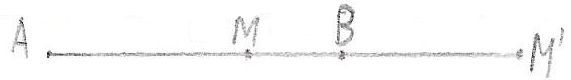
\includegraphics[scale=2]{sizigiArmonika}
	\caption{\textgreek{Συζυγή Αρμονικά σημεία Μ \& Μ'}}
	\label{fig:sizigiArmonika}
	\end{figure}
	
	\textbullet \quad (\figref{sizigiArmonika}) \textgreek{Δύο σημεία Μ και Μ', που διαιρούν εσωτερικά και εξωτερικά το τμήμα ΑΒ στον ίδιο λόγο, λέγονται συζυγή αρμονικά των Α και Β, αν τα τέσσερα σημεία είναι συνευθειακά και επίσης ισχύει ότι: } $\displaystyle  \frac{MA}{MB} = \frac{M'A}{M'B} $ \linebreak 
	\textbullet \quad \textgreek{Δύο (ή περισσότερα) ευθύγραμμα σχήματα λέγονται όμοια, όταν οι πλευρές τους είναι ανάλογες (ανάλογο μήκος) και οι γωνίες τους ίσες.} \linebreak
	\textbullet \quad \textgreek{Το ύψος} $\upsilon_a$ \textgreek{ενός τριγώνου } $\displaystyle A\overset{\triangle}{B}C$ \textgreek{ δίνεται από τον τύπο:} $\displaystyle \upsilon_a = \frac{2}{a}\sqrt{\tau(\tau -a)(\tau -b)(\tau -c)} , \tau$ \textgreek{: ημιπερίμετρος.} \linebreak 
	
	\uline{\textgreek{Αναλογίες}} \linebreak 
	\textbullet \quad $\displaystyle \frac{a}{b} = \frac{c}{d} \leftrightarrow ad = bc , \quad \frac{a}{b} = \frac{b}{c} \leftrightarrow b^2 = ac $ \linebreak 
	\textbullet \quad $\displaystyle \frac{a}{b} = \frac{c}{d} \leftrightarrow \frac{a}{c} = \frac{b}{d} $ \linebreak 
	\textbullet \quad $\displaystyle \frac{a}{b} = \frac{c}{d} \leftrightarrow \frac{a \pm b}{b} = \frac{c \pm d}{d}, \frac{a}{b} = \frac{c}{d} \leftrightarrow \frac{a}{a \pm b}= \frac{c}{c \pm d} $ \linebreak 
	\textbullet \quad $\displaystyle \frac{a}{b} = \frac{c}{d} = \ldots = \frac{k}{l} = \frac{a+c+\ldots +k}{b+d+\ldots + l} $ \linebreak 
	\textbullet \quad $\displaystyle  a \varpropto b \leftrightarrow a = \lambda \cdot b $ \linebreak 
	
		
	\subsection{Triangle} 
	
	\begin{figure}[H] 
	\centering
	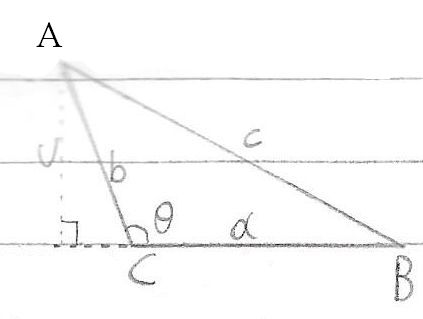
\includegraphics[scale=2]{trigono}
	\caption{Reference Triangle}
	\label{fig:trigono} % to able to reference the figure
	\end{figure}
	
	\textbullet \quad $ \Pi = a + b + c $  :  \textgreek{Περίμετρος} (See \figref{trigono}) \linebreak 
	\textbullet \quad $\displaystyle \epsilon = \frac{a \cdot \upsilon}{2} = \frac{ab\cdot sin \theta}{2} = \frac{r\Pi}{2} $  :  \textgreek{Εμβαδό τριγώνου} \linebreak 
	\textbullet \quad $\displaystyle \epsilon = \sqrt{\Tau (\Tau -a)(\Tau -b)(\Tau -c)} $  :  \textgreek{Τύπος του Ήρωνα, όπου} $\Tau$ \textgreek{ημιπερίμετρος τριγώνου} \linebreak 
	
	$r:$ \textgreek{η ακτίνα του εγγεγραμένου κύκλου του τριγώνου} \linebreak
	\textbullet \quad $\displaystyle S = \frac{\Pi}{2} = \frac{a + b + c}{2} $ \linebreak
	\textbullet \quad \textgreek{Για ισόπλευρο τρίγωνο έχουμε:} $\displaystyle \epsilon = \frac{\sqrt{3}}{2}a, \Pi = 3a$ , $a$  :  \textgreek{πλευρά} \linebreak

	\textbullet \quad $\displaystyle 30^o-60^o-90^o \ \text{triangle} \rightarrow 1:\sqrt{2}:2 $ \linebreak 
	\textbullet \quad $\displaystyle 45^o-45^o-90^o \ \text{triangle} \rightarrow 1:1:\sqrt{2} $ \linebreak 
	\textbullet \quad $\displaystyle \epsilon = \frac{abc}{4R} = \frac{1}{2}bc\cdot sinA = \frac{1}{2}ac\cdot sinB = \frac{1}{2}ab\cdot sinC $ $R: $ \textgreek{ακτίνα περιγεγγραμένου κύκλου του τριγώνου} \linebreak
	
	\uline{\textgreek{Ορθογώνιο Τρίγωνο}} \linebreak
	
	\begin{figure}[ht]
	\centering
	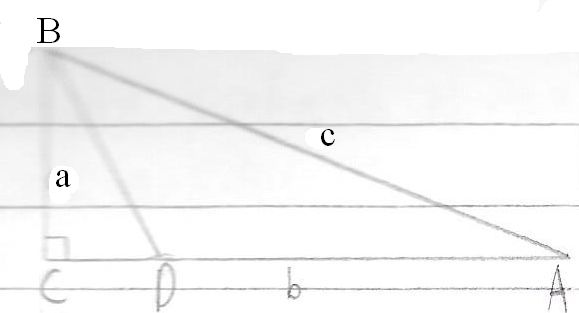
\includegraphics[scale=2]{orthTrigono}
	\caption{\textgreek{Ορθογώνιο Τρίγωνο}}
	\label{fig:orthTrigono}
	\end{figure}
	
	\textbullet \quad $\displaystyle  a^2 = b^2 + c^2 $  :  \textgreek{Πυθαγόρειο Θεώρημα} \linebreak 
 	\textbullet \quad $\displaystyle  a^2 = b^2 + c^2 - 2b\cdot AC, \text{in}\  A\overset{\triangle}{B}D $  \textgreek{: Γενίκευση Π.Θ. για} $\displaystyle \overset{\wedge}{A} < 90^o$, $AC = $ \textgreek{προβ}$_b c $ \linebreak
	\textbullet \quad \textgreek{Εάν} $\displaystyle \overset{\wedge}{A} > 90^o \rightarrow A\overset{\triangle}{B}C $ \textgreek{αμβλυγώνιο} $\displaystyle  \rightarrow a^2 = b^2 + c^2 +2b \cdot AC $ \linebreak 
	\textbullet \quad The maximum possible altitude of a right-angled triangle is half the hypotenuse. By inscribing the triangle into a circle to see this. \linebreak 
	
	\uline{\textgreek{1ο Θεώρημα Διαμέσων}} \linebreak
	\textbullet \quad $\displaystyle b^2 + c^2 = 2\mu_a^2 + \frac{a^2}{2} , a^2 + c^2 = 2\mu_b^2 + \frac{b^2}{2} ,\ a^2 + b^2 = 2\mu_c^2 + \frac{c^2}{2} $ \linebreak
	\uline{\textgreek{2ο Θεώρημα Διαμέσων}} \linebreak
	\textbullet \quad $\displaystyle b^2 -c^2 = 2a \cdot MD \ , MD = $ \textgreek{προβ}$_a \mu_a$ \linebreak 
	
	
	\subsection{Quadrilateral}
	
	\begin{figure}[ht]
	\centering
	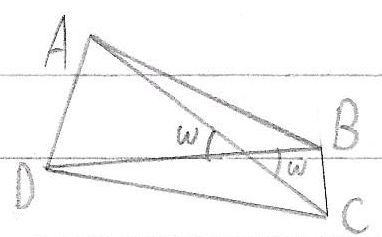
\includegraphics[scale=2]{kirtoTetrapleuro}
	\caption{\textgreek{Κυρτό Τετράπλευρο}}
	\label{fig:kirtoTetrapleuro}
	\end{figure}
	
	\textbullet \quad (\figref{kirtoTetrapleuro}) \textgreek{Το εμβαδό κυρτού τετραπλεύρου ισούται με το ημιγινόμενο των διαγωνίων του, πολ/μένο με το ημίτονο της γωνίας ω που αυτές σχηματίζουν: } $\displaystyle (ABCD) = 1/2 \cdot AC \cdot BC \cdot sin (\overset{\wedge}{\omega}) $ \linebreak 

	\uline{\textgreek{Ορθογώνιο Παραλληλόγραμμο}} \linebreak 
	\textbullet \quad $ \Pi = 2( \alpha + \beta) $ \linebreak 
	\textbullet \quad $ E= \alpha \cdot \beta $ \linebreak 
	
	\uline{\textgreek{Πλάγιο Παραλληλόγραμμο}} \linebreak 
	\textbullet \quad $ \Pi = 2(a+b) $ \linebreak 
	\textbullet \quad $\displaystyle  E = \alpha \cdot \upsilon = \alpha \beta \sin (\theta) $ \linebreak 
	
	\begin{figure}[ht]
	\centering
	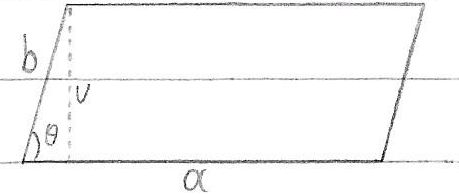
\includegraphics[scale=2]{plagioParal}
	\caption{\textgreek{Πλάγιο Παραλληλόγραμμο}}
	\label{fig:plagioParal}
	\end{figure}
	
	\uline{\textgreek{Ρόμβος}} \linebreak 
	\textbullet \quad $ \Pi = 4\alpha $ \linebreak 
	\textbullet \quad $\displaystyle E = \frac{\delta_1 \cdot \delta_2}{2} = \alpha \cdot \upsilon $ \linebreak 
	
	\begin{figure}[ht]
	\centering
	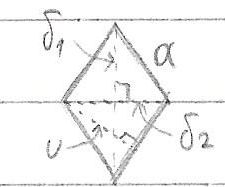
\includegraphics[scale=2]{romvos}
	\caption{\textgreek{Ρόμβος}}
	\label{fig:romvos}
	\end{figure}
	
	\uline{\textgreek{Τραπέζιο}} \linebreak  
	\textbullet \quad $\displaystyle \Pi = \alpha + \beta + \upsilon \cdot \left(\frac{1}{sin \theta} + \frac{1}{sin \phi} \right) $ \linebreak 
	\textbullet \quad $\displaystyle E = \frac{a + b}{2} \upsilon =\overleftrightarrow{E\text{\textgreek{Ζ}}} \cdot \upsilon $ \linebreak
	\textbullet \quad $\displaystyle \overleftrightarrow{E\text{\textgreek{Ζ}}} = \frac{a + b}{2} $ \textgreek{(διάμεσος) Η διάμεσος διέρχεται από τα μέσα των διαγωνίων του τραπεζίου.} $ BK = KD, A\Lambda = \Lambda C $. \linebreak 
	
	\begin{figure}[ht]
	\centering
	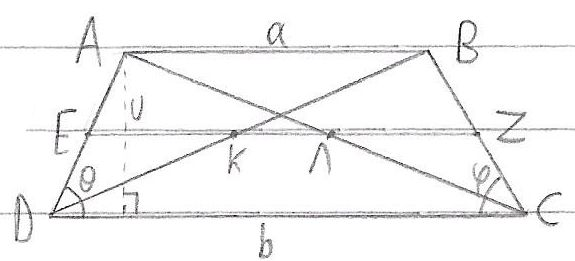
\includegraphics[scale=2]{trapezio}
	\caption{\textgreek{Τραπέζιο}}
	\label{fig:trapepzio}
	\end{figure}
	

	\subsection{Regular Polygon}	

	\textbullet \quad \textgreek{Ο λόγος των εμβαδών δύο όμοιων πολυγώνων, έστω Ε και Ε', ισούται με το τετράγωνο του λόγου ομοιότητας τους:} $\displaystyle \frac{a}{a'} = \frac{\upsilon_a}{\upsilon_{a'}} =\lambda \longrightarrow \frac{E}{E'} = \lambda^2 $ \linebreak 
	
	\begin{figure}[H]
	\centering
	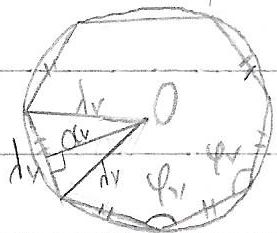
\includegraphics[scale=2]{poligono}
	\caption{\textgreek{Στοιχεία Κανονικού Πολυγώνου}}
	\label{fig:poligono}
	\end{figure}
	
	\textgreek{Σε κάθε κανονικό πολύγωνο ισχύουν οι σχέσεις:}
	\begin{enumerate}
	\item $\displaystyle a_v^2 + \frac{\lambda_v^2}{4} = R^2 $ 
	\item $\displaystyle  P_v = v\cdot \lambda_v $ \textgreek{: Περίμετρος} 
	\item $\displaystyle  \omega_v = \frac{360^o}{v} $ \textgreek{: Επίκεντρη γωνία} 
	\item $\displaystyle  E_v = \frac{1}{2} P_v \cdot a_v $ \textgreek{: Εμβαδό}  
	\item $\displaystyle  \phi_v = 180^o -\omega_v $ \textgreek{: Γωνία πολυγώνου} 
	\end{enumerate}		
	
	\textgreek{όπου} $\lambda_v:$ \textgreek{πλευρά πολυγώνου}, $R:$ \textgreek{ακτίνα κύκλου}, $a_v:$ \textgreek{απόστημα}, $v:$ \textgreek{πλήθος πλευρών πολυγώνου} \linebreak 
	\textbullet \quad \textgreek{Άθροισμα εσωτερικών γωνιών πολυγώνου}: $(2v-4)L$ \linebreak 
	\textbullet \quad \textgreek{Άθροισμα εξωτερικών γωνιών κυρτού πολυγώνου}: $4L$ \linebreak
	
	
	\subsection{Stereometry - Polyhedron}

	\textbullet \quad \textgreek{Θεώρημα του} Euler (Euler's formula) \textgreek{για τα πολύεδρα}: $K + E = A + 2$ \linebreak
	K: \textgreek{πλήθος κορυφών}, E: \textgreek{πλήθος εδρών}, A: \textgreek{πλήθος ακμών} \linebreak
	\textbullet \quad $\displaystyle  A= \frac{\nu E}{2} $, $\nu$  :  \textgreek{αριθμός πλευρών κάθε έδρας. Κάθε έδρα έχει και ν κορυφές} \linebreak 
	\textbullet \quad \textgreek{Για μια επιφάνεια} $A$ \textgreek{η στερεά γωνία} $\omega$ \textgreek{που την περιλαμβάνει ορίζεται ως}: $\displaystyle  \omega = \frac{A'}{ R^2} \ (sr)$ \linebreak 
	\textgreek{όπου} $A'$ \textgreek{η προβολή του Α σε σφαίρα ακτίνας} $R$. \linebreak 
	\textgreek{Μονάδα μέτρησης}: steradians (sr) \linebreak 
	
	\begin{figure}[H]
	\centering
	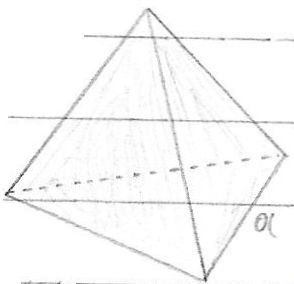
\includegraphics[scale=2]{tetrahedron}
	\caption{\textgreek{Στοιχεία Τετραέδρου}}
	\label{fig:tetrahedron}
	\end{figure}
	
	\uline{\textgreek{Τετράεδρο}} \linebreak 
	\textbullet \quad \textgreek{Εμβαδό κανονικού τετραέδρου: } $\displaystyle E =\sqrt{3} a^2 $ \linebreak 
	\textbullet \quad \textgreek{Όγκος κανονικού τετραέδρου: } $\displaystyle V = \frac{\sqrt{2}a^3}{12} $ \linebreak 

	\begin{figure}[H]
	\centering
	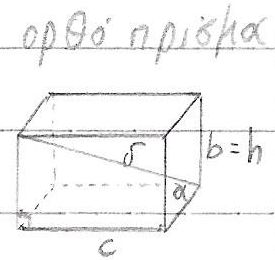
\includegraphics[scale=2]{orthParallilepipedo}
	\caption{\textgreek{Στοιχεία Ορθογωνίου Παραλληλεπιπέδου}}
	\label{fig:orthParallilepipedo}
	\end{figure}	
	
	\uline{\textgreek{Ορθογώνιο Παραλληλεπίπεδο}} \linebreak 
	\textbullet \quad \textgreek{Όγκος}: $\displaystyle V = a\cdot b \cdot c = E_B \cdot c$ \linebreak 
	\textbullet \quad \textgreek{Διαγώνιος}: $\displaystyle \delta^2 = a^2 + b^2 + c^2 $ \linebreak 
	\textbullet \quad \textgreek{Εμβαδό ολικής επιφάνειας}: $\displaystyle E_0 = E_\pi + 2E_B$  , $E_B$  :  \textgreek{εμβαδό βάσης} \linebreak
	
	\begin{figure}[H]
	\centering
	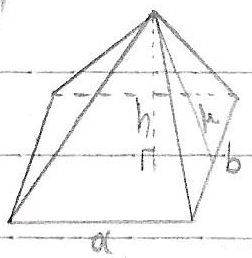
\includegraphics[scale=2]{pyramid}
	\caption{\textgreek{Πυραμίδα}}
	\label{fig:pyramid}
	\end{figure}
	
	\uline{\textgreek{Πυραμίδα}} \linebreak 
	\textbullet \quad \textgreek{Εμβαδό}: $\displaystyle E = ab + a\sqrt{\left(\frac{b}{2} \right)^2 + h^2} + b\sqrt{\left(\frac{a}{2}\right)^2 + h^2} $ \linebreak 
	\textbullet \quad \textgreek{Όγκος}: $\displaystyle  V = \frac{E_B h}{3} , \ E_B$  :  \textgreek{εμβαδό βάσης} \linebreak 	
	
	\uline{\textgreek{Κανονική Πυραμίδα}} \linebreak 
	\textgreek{(πυραμίδα που η βάση της είναι κανονικό πολύγωνο και τα πλευρικά ύψη είναι όλα ίσα σε μήκος.)} \linebreak 
	\textbullet \quad \textgreek{Εμβαδό παράπλευρης επιφάνειας}: $\displaystyle E_\pi = \tau \cdot \mu $ \linebreak 
	\textbullet \quad \textgreek{Εμβαδό ολικής επιφάνειας}: $\displaystyle E_0 = \tau(\mu + \alpha) $ \linebreak  
	$\tau$  :  \textgreek{ημιπερίμετρος βάσης}, $\mu$  :  \textgreek{παράπλευρο / λοξό ύψος} \linebreak
	
	\begin{figure}[H]
	\centering
	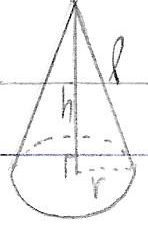
\includegraphics[scale=2]{cone}
	\caption{\textgreek{Στοιχεία Κώνου}}
	\label{fig:cone}
	\end{figure}	
			
	\uline{\textgreek{Κώνος}} \linebreak 
	\textbullet \quad \textgreek{Εμβαδό παράπλευρης επιφάνειας}: $\displaystyle E_\pi = \pi r l $ \linebreak  
	\textbullet \quad  \textgreek{Συνολικό εμβαδό}: $\displaystyle E_0 = \pi rl + \pi r^2 $ , $l$  :  \textgreek{λοξό ύψος} \linebreak 
	\textbullet \quad \textgreek{Όγκος κώνου}: $\displaystyle V = \frac{\pi r^2 h}{3} $ , $r$  :  \textgreek{ακτίνα βάσης} \linebreak  

	\begin{figure}[H]
	\centering
	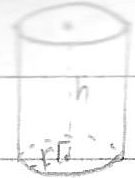
\includegraphics[scale=2]{cylinder}
	\caption{\textgreek{Κύλινδρος}}
	\label{fig:cylinder}
	\end{figure}	
	
	\uline{\textgreek{Κύλινδρος}} \linebreak 
	\textbullet \quad \textgreek{Παράπλευρο εμβαδόν}: $\displaystyle E_\pi = 2\pi rh$ \linebreak  
	\textbullet \quad \textgreek{Ολικό εμβαδό}: $\displaystyle E_0 = 2\pi r^2 +2\pi rh$ \linebreak  
	\textbullet \quad \textgreek{Όγκος}: $\displaystyle V = \pi r^2h$ \linebreak 
	\textbullet \quad \textgreek{Περίμετρος (έπειτα από πλάγια προβολή σε επίπεδο} $ \Pi = 2(2r + h) $ \linebreak 
	
	\uline{\textgreek{Σφαίρα}} \linebreak 
	\textbullet \quad \textgreek{Εμβαδόν}: $\displaystyle E = 4\pi r^2$ \linebreak  
	\textbullet \quad \textgreek{Όγκος}: $\displaystyle V = \frac{4}{3}\pi r^3 $ \linebreak 
	
	\uline{\textgreek{Μέτρηση κόλουρης (Ισοσκελούς) Πυραμίδας}} \linebreak 
	\textbullet \quad \textgreek{Εμβαδό παράπλευρης επιφάνειας}: $\displaystyle E_\pi = (\tau +\tau') \mu $ \\ 
		$\tau, \tau'$  :  \textgreek{οι ημιπερίμετροι των βάσεων, μ: παράπλευρο ύψος} \linebreak 
	\textbullet \quad \textgreek{Εμβαδό ολικής επιφάνειας}: $\displaystyle E = E_\pi + E_B + E_{B'} $ \\ 
		$E_B$  :  \textgreek{Εμβαδό μεγάλης βάσης}, $E_{B'}$  :  \textgreek{Εμβαδό μικρής βάσης} \linebreak 

	\begin{figure}[H]
	\centering
	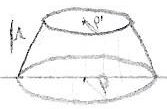
\includegraphics[scale=3]{coneFrustum}
	\caption{\textgreek{Κόλουρος κώνος}}
	\label{fig:coneFrustum}
	\end{figure}		
	
	\uline{\textgreek{Μέτρηση Κόλουρου Κώνου}} \linebreak 
	\textbullet \quad \textgreek{Εμβαδό παράπλευρης επιφάνειας}: $\displaystyle E_\pi = \pi \cdot \mu (\rho + \rho') $ \\ 
	$\mu$  :  \textgreek{παράπλευρο ύψος}, $\rho, \rho'$  :  \textgreek{μεγάλη και μικρή ακτίνα αντίστοιχα}	\linebreak  
	\textbullet \quad \textgreek{Ολικό εμβαδόν}: $\displaystyle E_0 = E_\pi + \pi(\rho^2 + \rho^{'2})$ \linebreak  
	\textbullet \quad \textgreek{Όγκος κόλουρου κώνου}: $\displaystyle V = \frac{\pi \upsilon}{3} \left( \rho^2 + \rho^{'2} + \rho	\cdot \rho' \right) $ \linebreak 
	
	
	\subsection{Line}
	
	\textbullet \quad \textgreek{Γενική μορφή εξίσωσης ευθείας:} $\displaystyle Ax + By + \Gamma = 0$, \textgreek{όπου Α και Β δεν είναι συγχρόνως ίσα με το μηδέν.} \linebreak 
	\textbullet \quad \textgreek{Κανονική μορφή εξίσωσης ευθείας:} $\displaystyle y= m\cdot x + b$, $b$  :  $y$-intercept, $m$  :  \textgreek{συντελεστής διεύθυνσης ευθείας που διέρχεται από τα σημεία} $A(x_1, y_1)$ \textgreek{και} $B(x_2, y_2)$, $\displaystyle m = \frac{y_2 -y_1}{x_2-x_1} = \frac{y_1 -y_2}{x_1 -x_2} = \frac{y}{x} $ \linebreak 
	\textbullet \quad \textgreek{Εξίσωση ευθείας όταν δίνονται δύο σημεία της:} \\
	$ y - y_1 = \frac{y_2-y_1}{x_2-x_1} \cdot (x-x_1) $ \linebreak 
	\textbullet \quad \textgreek{Η γενική μορφή εξίσωσης ευθείας σε δύο διαστάσεις είναι:} \\ 
	$\displaystyle \frac{x-x_{\text{\textgreek{αρχ}}}}{x_{\text{\textgreek{τελ}}} - x_{\text{\textgreek{αρχ}}}} = \frac{y - y_{\text{\textgreek{αρχ}}}}{y_{\text{\textgreek{τελ}}} - y_{\text{\textgreek{αρχ}}}}$, \linebreak 
	\textgreek{μορφή ισοδύναμη με} $\displaystyle  m = \frac{y_{\text{\textgreek{τελ}}} -y_{\text{\textgreek{αρχ}}}}{x_{\text{\textgreek{τελ}}}-x_{\text{\textgreek{αρχ}}}} $ \linebreak 
	\textbullet \quad \textgreek{Γενική μορφή εξίσωσης ευθείας σε τρείς διαστάσεις:} \\ 
	$\displaystyle  \frac{x - x_{\text{\textgreek{αρχ}}}}{x_{\text{\textgreek{τελ}}}- x_{\text{\textgreek{αρχ}}}} = \frac{y - y_{\text{\textgreek{αρχ}}}}{y_{\text{\textgreek{τελ}}} - y_{\text{\textgreek{αρχ}}}} = \frac{z - z_{\text{\textgreek{αρχ}}}}{z_{\text{\textgreek{τελ}}} - z_{\text{\textgreek{αρχ}}}} $ \linebreak 
	\textbullet \quad \textgreek{Πολική μορφή εξίσωσης ευθείας}: $\displaystyle r = \frac{mr\cos \theta + b}{\sin \theta} $ \textgreek{όταν θ = 0 δεν ορίζεται πολική μορφή εξίσωσης ευθείας} \linebreak 
	\textbullet \quad $\displaystyle m_1 = m_2 \leftrightarrow line 1 \parallel line 2$ \linebreak 
	\textbullet \quad $\displaystyle m_1 \cdot m_2 = -1 \leftrightarrow line 1 \perp line 2 $ \linebreak 
	\textbullet \quad $\displaystyle \tan (\theta) = \left| \frac{m_1 -m_2}{1+m_1 \cdot m_2} \right| $  :  \textgreek{Γωνία θ μεταξύ 2 καμπυλών ευθειών} $m_1, m_2$ \textgreek{: κλίσεις των καμπυλών στο σημείο επαφής τους, ή οι κλίσεις των ευθειών} \linebreak 
	\textbullet \quad \textgreek{Απόσταση σημείου} $M(x_0,y_0)$ \textgreek{και ευθείας} $\displaystyle \epsilon: Ax +By +\Gamma = 0: d(M,\epsilon) = \frac{\left|Ax_0 +By_0 +\Gamma \right|}{\sqrt{A^2 +B^2}} $ \linebreak 

	
	\subsection{Miscellaneous} 
	
	\textbullet \quad $n \in \mathbb{N}^*$ chords drawn in a circle in such a way that each chord intersects each other, but no three intersect at one point, cut the circle into $\displaystyle \frac{n^2 + n + 2}{2} $ regions. \linebreak 
	\textbullet \quad \textgreek{Η γωνία που σχηματίζεται από μια χορδή κύκλου και την εφαπτομένη στο άκρο της χορδής ισούται με την εγγεγραμένη που βαίνει στο τόξο της χορδής. - Γωνία χορδής και εφαπτομένης} \linebreak  
	\textbullet \quad \textgreek{Όταν ένα τετράπλευρο έχει δύο απέναντι γωνίες του παραπληρωματικές και μια πλευρά του φαίνεται από τις απέναντι κορυφές υπό ίσες γωνίες, τότε είναι εγγράψιμο σε κύκλο.} \linebreak  
	\textbullet \quad An open polygon with $n$ sides and $k$ vertexes at infinity will have $(n-k)$ internal angles. \linebreak 
	\textbullet \quad \uline{Orthogonality} is the relation of two lines at right angles to one another (perpendicularity), and the generalization of this relation into n dimensions; and to a variety of mathematical relations thought of as describing non-overlapping, uncorrelated, or independent objects of some kind. \linebreak 
	\textbullet \quad $1$ arcminute is $\frac{1}{60}$th of a degree. $1$ arcsecond is $\frac{1}{3600}$th of a degree. 
	
	
	\pagebreak
	

	\section{Conic Sections}	
	
	\subsection{Circle}

	\textbullet \quad \textgreek{Αν δύο χορδές AB, ΓΔ, ή οι προεκτάσεις τους τέμνονται σε ένα σημείο Ρ, τότε ισχύει: } $\displaystyle PA\cdot PB = P\Gamma \cdot P\Delta $. \textgreek{Στην ειδική περίπτωση της εφαπτομένης, όπου τα σημεία τομής ταυτίζονται (έστω Γ, Δ} $\equiv$ \textgreek{Ε), το θεώρημα ισχύει: } $ PE^2 = PA \cdot PB.$ \textgreek{Εάν ΟΡ = δ τότε:} $\delta^2 -R^2$ \textgreek{λέγεται δύναμη του Ρ ως προς τον (Ο,R) και συμβολίζεται} $\displaystyle \Delta_{(O,R)} = \delta^2 -R^2 = OP^2 -R^2 $ \linebreak 
	\textbullet \quad $\displaystyle (x-x_0)^2 + (y-y_0)^2 = r^2 $ \textgreek{: Εξίσωση κύκλου, κέντρο: } $ O(x_0,y_0)$, \textgreek{ακτίνα:} $r$ \textgreek{Όταν κέντρο είναι:} $K(0,0)$ \textgreek{,τότε:} $ x^2 + y^2 = r^2$ \linebreak 
	\textbullet \quad $\displaystyle x^2 + y^2 +Ax +By +C = 0, A^2 +B^2 -4C > 0$  :  \uline{\textgreek{Γενικευμένη εξίσωση κύκλου}} \\ \textgreek{κέντρο}: $\displaystyle \left(-\frac{A}{2}, -\frac{B}{2} \right)$ \textgreek{, ακτίνα: } $\displaystyle r=\frac{\sqrt{A^2+B^2-4C}}{2} , A = -2x_0, B=-2y_0$ \linebreak
	
	\textbullet \quad \uline{\textgreek{Εξίσωση κύκλου σε πολικές συντεταγμένες}}: $\displaystyle r^2 -2rr_0 cos (\phi - \phi_0) + r_0^2 = R^2$, \textgreek{ακτίνα:} $R$ \linebreak 
	\textbullet \quad $\displaystyle L = 2\pi r$ \textgreek{: Περιφέρεια κύκλου} \linebreak 
	\textbullet \quad $\displaystyle E = \pi r^2 $  :  \textgreek{Εμβαδό} \linebreak 
	\textbullet \quad $\displaystyle \pi = \frac{\text{ \textgreek{περιφέρεια του κύκλου} }}{\text{ \textgreek{διάμετρος του κύκλου} }} = 3.14\ 159\ $ \linebreak 
	\textbullet \quad $\displaystyle \frac{\text{\textgreek{Κεντρική γωνία θ τόξου (σε }} ^o \text{\textgreek{ ή} rad})}{360^o \text{\textgreek{ ή }} 2\pi}  = \frac{\text{\textgreek{περιφέρεια τόξου}}\ L}{\text{\textgreek{περιφέρεια κύκλου}}: 2\pi r} $ \linebreak 
	\textbullet \quad $\displaystyle  \text{\textgreek{ακτίνιο}} (rad) = $ \textgreek{τόξο μήκους} $r$ \textgreek{(ίσο με την ακτίνα)} \linebreak 
	\textbullet \quad $\displaystyle  \frac{180^o}{\mu} = \frac{\pi}{\alpha} $ \\ \textgreek{μ: μέτρο γωνίας σε μοίρες,  α: μέτρο γωνίας σε ακτίνια} \linebreak 
	\textbullet \quad $\displaystyle L = r\cdot a $ \textgreek{ή} $\displaystyle L = \frac{\pi \mu r}{180^o} $  :  \textgreek{Μήκος τόξου} \linebreak
	\textbullet \quad $\displaystyle E = \frac{1}{2} r^2 \alpha $ \textgreek{ή} $\displaystyle E = \frac{\mu \pi r^2}{360} $  :  \textgreek{Εμβαδό κυκλικού τομέα ακτίνας } $r$, \textgreek{τόξου θ} \linebreak 

	\begin{figure}[H]
	\centering
	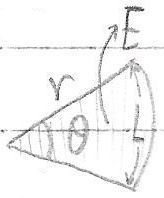
\includegraphics[scale=2]{toxo}
	\caption{\textgreek{Τόξο κύκλου}}
	\label{fig:Toxo}
	\end{figure}
	
	\uline{\textgreek{Παραμετρικές εξισώσεις κύκλου}} \linebreak
	\textbullet \quad $\displaystyle x=r\cdot \cos (\theta), y = r\cdot \sin (\theta), \theta = [0, 2\pi) $ \linebreak 
	\textbullet \quad $\displaystyle r = \frac{abc}{4\sqrt{S(S-a)(S-b)(S-c)}} $ \textgreek{: Κύκλος ακτίνας} $r$ \textgreek{περιγεγγραμένος σε} $\displaystyle A\overset{\wedge}{B}\Gamma$ \linebreak 
	\textbullet \quad \textgreek{Εξίσωση εφαπτομένης κύκλου με κέντρο την αρχή των αξόνων: } $\displaystyle  x\cdot x_1 + y\cdot y_1 = r^2 \text{\qquad} (x_1, y_1) $ \textgreek{: σημείο επαφής κύκλου - ευθείας}. \linebreak 	
	
	\subsection{Parabola}
	
	\textbullet \quad \uline{\textgreek{Παραβολή}}: \textgreek{ορίζεται ως ο Γ.Τ. των σημείων ενός επιπέδου που ισαπέχουν από δεδομένη ευθεία δ - τη διευθετούσα και σημείο Ε του επιπέδου, εκτός της ευθείας δ.} \linebreak 
		\textbullet \quad $|r|$  :  \textgreek{απόσταση εστίας από τη διευθετούσα}, $r = \frac{1}{2a} $  :  \textgreek{παράμετρος παραβολής ίση με την απόσταση της εστίας από τη διευθετούσα} \linebreak 
	\textbullet \quad  \textgreek{Εξίσωση παραβολής με εστία} $\displaystyle E(\frac{r}{2}, 0)$ \textgreek{και διευθετούσα} $\displaystyle x=-\frac{r}{2}$ \textgreek{σε καρτεσιανές συντεταγμένες είναι}: $\displaystyle y^2 = 2rx$. \linebreak 
	\textbullet \quad \textgreek{Εξίσωση παραβολής με εστία} $\displaystyle E(0, \frac{r}{2}) \text{\textgreek{\ και\ }} \delta: y = -\frac{r}{2}$ \textgreek{σε καρτεσ. συντ. είναι:} $\displaystyle x^2 = 2ry$. \linebreak 
	\textbullet \quad \uline{\textgreek{Γενικής μορφή εξίσωσης παραβολής}}: $ y = ax^2 +bx +c $. \textgreek{ή στη} vertex \textgreek{μορφή της}: $ y=a(x-h)^2 + k $ \textgreek{Η καμπύλη αυτή είναι παραβολή αν} $\displaystyle 4ac = b^2$ \textgreek{και τουλάχιστον ένα των} $a,c$ \textgreek{διάφορο του μηδενός.}\linebreak 
	\textgreek{έχει κορυφή το σημείο} $\displaystyle K\left( \frac{-\beta}{2\alpha}, \frac{-\Delta}{4\alpha} \right)$, \textgreek{όπου} $\displaystyle \Delta = \beta^2 -4\alpha \gamma $ \linebreak 
	\textgreek{εστία } $ E\left( \frac{1 - \Delta}{4a} \right) $ \linebreak 
	\textgreek{και διευθετούσα } $ y = c - \frac{b^2 + 1}{4a} $ \linebreak 
	\textgreek{Η γραφική παράσταση της παραβολής} $\displaystyle y=\alpha x^2+\beta x +\gamma, \alpha \neq 0$, \textgreek{άξονα συμμετρίας την κατακόρυφη γραμμή που διέρχεται από την κορυφή Κ και έχει εξίσωση} $\displaystyle x=\frac{-\beta}{2\alpha} $. $ \text{\textgreek{Εάν\ }} \alpha >0\ \eta \ y $ \textgreek{παίρνει ελάχιστη τιμή το} $y_k$, \textgreek{ενώ αν} $\alpha<0$ \textgreek{η} $y$ \textgreek{παίρνει ελάχιστη τιμή το} $y_k$. \linebreak 
	\textbullet \quad \textgreek{Εφαπτομένη παραβολής στο} $\displaystyle A(x_0, y_0) \quad y^2 = 2rx$, \textgreek{είναι}: $\displaystyle yy_0 = r(x+x_0)$ \linebreak 
	\textbullet \quad \textgreek{Εφαπτομένη παραβολής στο} $\displaystyle A(x_0, y_0) \quad x^2 = 2ry$, \textgreek{είναι}: $\displaystyle xx_0 = r(y+y_0)$ \linebreak 
			
	\subsection{Ellipse}
	
	\textbullet \quad \uline{\textgreek{Έλλειψη}} \textgreek{είναι ο Γ.Τ. των σημείων του επιπέδου των οποίων το άθροισμα των αποστάσεων από δύο σταθερά σημεία - τις εστίες της έλλειψης - Ε και Ε', είναι σταθερό, ίσο με 2α και μεγαλύτερο της εστιακής απόστασης ΕΕ'} \linebreak 
	\textbullet \quad \textgreek{Σε κάθε έλλειψη ισχύει} $(ME')+(ME)=2\alpha$, \textgreek{Μ: σημείο της έλλειψης} \linebreak 
	\textbullet \quad \textgreek{Εξίσωση έλλειψης με εστίες} $E'(-\gamma,0)$ \textgreek{και} $E(\gamma,0)$ \textgreek{είναι} $\displaystyle \frac{x^2}{\alpha^2} + \frac{y^2}{\beta^2} = 1$, \textgreek{όπου} $\displaystyle \beta = \sqrt{\alpha^2 - \gamma^2} $ \linebreak 
	\textbullet \quad \textgreek{Εξίσωση έλλειψης με εστίες} $E'(0, -\gamma)$ \textgreek{και} $E(0,\gamma)$ \textgreek{είναι} $\displaystyle \frac{x^2}{\beta^2} + \frac{y^2}{\alpha^2} = 1$, \textgreek{όπου} $\displaystyle \beta = \sqrt{\alpha^2 - \gamma^2} $ \linebreak 
	\textbullet \quad \textgreek{Μεγάλος άξονας = 2α} \linebreak 
	\textbullet \quad \textgreek{Μικρός άξονας = 2β} \linebreak 
	\textbullet \quad $\displaystyle \epsilon = \frac{\gamma}{\alpha} $ \textgreek{εκκεντρότητα έλλειψης } $<1$ \linebreak 
	\textbullet \quad $\displaystyle \frac{\beta}{\alpha} = \sqrt{1-\epsilon^2} $ \linebreak 
	\textbullet \quad $2\beta \leq ($ \textgreek{διάμετρος έλλειψης} $\leq 2\alpha$ \linebreak 
	\textbullet \quad $\displaystyle x=\alpha \cos (\phi)$ , $\quad y=\beta \sin (\phi) $  :  \textgreek{Παραμετρικές εξισώσεις έλλειψης} \linebreak 
	\textbullet \quad \textgreek{2γ: εστιακή απόσταση} \linebreak 
	\textbullet \quad \textgreek{Γενική μορφή εξίσωσης έλλειψης:} $\displaystyle \frac{(x-x_0)^2}{a^2} +\frac{(y-y_0)^2}{b^2} = 1$, \textgreek{κέντρο} $K = (x_0, y_0), E'(x_0 -\gamma, 0), E(x_0 + \gamma,0)$ \linebreak 
	\textbullet \quad \textgreek{Εφαπτομένη έλλειψης} $\displaystyle \frac{x^2}{\alpha^2} + \frac{y^2}{\beta^2} = 1$, \textgreek{είναι}: $ \frac{xx_0}{\alpha^2} + \frac{yy_0}{\beta^2} = 1$ \textgreek{όπου} $A(x_0, y_0) $ \textgreek{σημείο επαφής}. \linebreak 
	\textbullet \quad \textgreek{Εφαπτομένη έλλειψης} $\displaystyle \frac{x^2}{\beta^2} + \frac{y^2}{\alpha^2} = 1$, \textgreek{είναι}: $ \frac{xx_0}{\beta^2} + \frac{yy_0}{\alpha^2} = 1$ \linebreak 
	\textbullet \quad \textgreek{Εμβαδό έλλειψης:} $A = \pi \alpha \beta$ \linebreak 
	\textbullet \quad \textgreek{Σημείο} $(x_0, y_0)$ \textgreek{εντός έλλειψης εάν}: $\displaystyle \frac{x_0^2}{\beta^2} + \frac{y_0^2}{\alpha^2} < 1 $ \linebreak 
	
	\subsection{Hyperbola} 
	
	\textbullet \quad \uline{\textgreek{Υπερβολή}} \textgreek{είναι ο Γ.Τ. των σημείων του επιπέδου των οποίων η απόλυτη τιμή της διαφοράς των αποστάσεων από τις εστίες Ε και Ε' είναι σταθερή, ίση με 2α και μικρότερη της εστιακής απόστασης (ΕΕ')}. \linebreak 
	\textbullet \quad \textgreek{Εστιακή απόσταση} $= 2\gamma$ \linebreak 
	\textbullet \quad \textgreek{Ένα σημείο Μ είναι σημείο της υπερβολής ανν} $\displaystyle  \left| (ME') -(ME) \right| = 2\alpha $. \linebreak 
	\textbullet \quad \textgreek{Ισχύει} $ \left| (ME') -(ME) \right| < (EE')$, \textgreek{δλδ.} $\displaystyle 2\alpha < 2\gamma \leftrightarrow \alpha < \gamma $ \linebreak 
	\textbullet \quad \textgreek{Εξίσωση υπερβολής με} $E(\gamma, 0)$ \textgreek{και} $E'(-\gamma, 0)$ \textgreek{είναι}: $\displaystyle \frac{x^2}{\alpha^2} - \frac{y^2}{\beta^2} = 1, \quad \beta = \sqrt{\gamma^2 -\alpha^2} $. \textgreek{Αν έχει εστίες Ε(0,-γ) και Ε'(0,γ) τότε η εξίσωση της είναι:} $ \frac{y^2}{\alpha^2} -\frac{x^2}{\beta^2} = 1$. \textgreek{Κέντρο κανονικής μορφής υπερβολής (0,0)} \linebreak 
	\textbullet \quad \textgreek{Αν α = β έχουμε την ισοσκελής υπερβολής:} $x^2 -y^2 = \alpha^2 $ \linebreak 
	\textbullet \quad \textgreek{Υπάρχουν δύο ασύμπτωτες της υπερβολής, όπου για την κανονικής μορφής υπερβολή είναι}: $ y= -\frac{\beta}{\alpha} x $ \textgreek{και} $y = \frac{\beta}{\alpha} x $ \uline{\textgreek{ανν}} $\displaystyle |\lambda| < \beta / \alpha$ \textgreek{όπου λ: συντελεστής διεύθυνσης ασύμπτωτης.} \linebreak 
	\textgreek{Για την υπερβολή με εξίσωση} $\frac{y^2}{\alpha^2} - \frac{x^2}{\beta^2} = 1$ \textgreek{οι ασύμπτωτες της είναι: } $y=\frac{\alpha}{\beta}x$ \textgreek{και} $y=-\frac{\alpha}{\beta}x$ \linebreak 
	\textbullet \quad $\displaystyle \epsilon = \frac{\gamma}{\alpha} (>1)$ \textgreek{: Εκκεντρότητα υπερβολής} \linebreak 
	\textbullet \quad $\displaystyle \frac{\beta}{\alpha} = \sqrt{\epsilon^2 -1}$ \linebreak 
	\textbullet \quad \textgreek{Εφαπτομένη υπερβολής} $\displaystyle \frac{x^2}{\alpha^2} - \frac{y^2}{\beta^2}$ \textgreek{στο} $M(x_0, y_0)$ \textgreek{είναι}: $\displaystyle  \frac{xx_0}{\alpha^2} -\frac{yy_0}{\beta^2} = 1$ \textgreek{ενώ η εφαπτομένη της υπερβολής} $\displaystyle \frac{y^2}{\alpha^2} - \frac{x^2}{\beta^2} = 1 $ \textgreek{είναι}: $\displaystyle \frac{yy_0}{\alpha^2} -\frac{xx_0}{\beta^2} = 1$ \linebreak 
	\textbullet \quad $\displaystyle d(M,\epsilon_1) \cdot d(M,\epsilon_2) = \frac{\alpha^2 \beta^2}{\alpha^2 \beta^2}$  :  \textgreek{Το γινόμενο των αποστάσεων ενός σημείου της υπερβολής από τις ασύμπτωτες της είναι σταθερό.} \linebreak

	
	\pagebreak
		
	
	\section{Calculus / Mathematical Analysis}

	\subsection{Limits}
	
	\textbullet \quad \uline{Existence of a limit} of a function $f(x)$ when: \linebreak 
	$\displaystyle \lim_{x\to c} f(x) = L \Leftrightarrow \left( \lim_{x\to c^-} f(x) = L \right) \land \left( \lim_{x\to c^+} f(x) = L \right) $ \linebreak 
	A function may have a limit at a point of its domain, but a different, or no value at that point. The limit describes the behavior of the function, as the latter tends towards a certain point. \linebreak 
	\textbullet \quad Suppose $\displaystyle f: \mathbb{R} \rightarrow \mathbb{R} \land x_0, L \in \mathbb{R}$. The limit of $f$, as $x$ approaches $x_0$ is $L$ and is written: $\displaystyle \lim_{x\to x_0} f(x) = L$. \linebreak 
	\textbullet \quad If the following property holds $\displaystyle \forall \epsilon \in \mathbb{R}^+ \exists \delta \in \mathbb{R}$ s.t. $\forall x \in \mathbb{R}( 0 < |x-x_0| < \delta $ implies $|f(x) -L| < \epsilon )$, then the value of the limit does not depend on the value of $f(x_0)$, nor even that $x_0$ be in the domain of $f$, i.e. the limit does not depend on $f(x_0)$ being well - defined. ($\epsilon$ = "error", $\delta$ = "distance") \linebreak \textgreek{Όταν η παραπάνω ιδιότητα ισχύει, τότε η} $f$ \textgreek{έχει στο} $x_0$ \textgreek{όριο το} $L \in \mathbb{R}$. \linebreak 
	\textbullet \quad $\displaystyle \lim_{x\to x_0} f(x) = L \leftrightarrow \lim_{x\to x_0^-} f(x) = \lim_{x\to x_0^+} f(x) = L $ \linebreak 
	\textbullet \quad $\displaystyle \lim_{x\to x_0} f(x) = L \leftrightarrow \lim_{x\to x_0} (f(x) - L) = 0 $ \linebreak 
	\textbullet \quad $\displaystyle \lim_{x\to x_0} f(x) = L \leftrightarrow \lim_{h\to 0} f(x_0 + h) = L $ \linebreak 
	\textbullet \quad $\displaystyle \lim_{x\to x_0} x = x_0$ \linebreak 
	\textbullet \quad $\displaystyle \lim_{x\to x_0} c = c$ \linebreak 
	\textbullet \quad $\displaystyle \lim_{x\to x_0} f(x) > 0 \rightarrow f(x) > 0 $ \textgreek{κοντά στο} $x_0$ \linebreak 
	\textbullet \quad $\displaystyle \lim_{x\to x_0} f(x) < 0 \rightarrow f(x) < 0 $ \textgreek{κοντά στο} $x_0$ \linebreak 
	\textbullet \quad \textgreek{Αν οι} $f,g$ \textgreek{έχουν όριο στο} $x_0$ \textgreek{και} $f(x) \leq g(x)$, \textgreek{κοντά στο} $x_0$, \textgreek{τότε}: $\displaystyle \lim_{x\to x_0} f(x) \leq \lim_{x\to x_0} g(x) $ \linebreak 
	\textbullet \quad \textgreek{Αν υπάρχουν τα πραγματικά όρια των} $f$ \textgreek{και} $g$ \textgreek{στο} $x_0$, \textgreek{τότε}: 
	\begin{itemize}
		\renewcommand{\labelitemi}{$\rightarrow$}
	\item $\displaystyle \lim_{x\to x_0} f(x) = L \leftrightarrow \frac{|L|}{2} < |f(x)| < \frac{3}{2} |L| $ \linebreak 
	\item $\displaystyle \lim_{x\to x_0} \sqrt[k]{f(x)} = \sqrt[k]{\lim_{x\to x_0} f(x)}$, \textgreek{εφόσον} $f(x) \geq 0$ \textgreek{κοντά στο} $x_0$ (Well defined radical)
	\end{itemize}
	\textbullet \quad $\displaystyle \lim_{x\to x_0} (k f(x)) = k\lim_{x\to x_0} f(x), \ \forall k \in \mathbb{R}$ \linebreak 
	\textbullet \quad $\displaystyle \lim_{x\to x_0} \left(f(x) \pm g(x)\right) = \lim_{x\to x_0} f(x) \pm \lim_{x\to x_0} g(x) $ \linebreak 
	\textbullet \quad $\displaystyle \lim_{x\to x_0} \left( f(x) \cdot g(x) \right) = \lim_{x\to x_0} f(x) \cdot \lim_{x\to x_0} g(x) $ \linebreak 
	\textbullet \quad $\displaystyle \lim_{x\to x_0} \frac{f(x)}{g(x)} = \frac{\lim_{x\to x_0} f(x)}{\lim_{x\to x_0} g(x)} $, \textgreek{εφόσον} $\lim_{x\to x_0} g(x) \neq 0$ \linebreak 
	\textbullet \quad $\displaystyle \lim_{x\to x_0} |f(x)| = |\lim_{x\to x_0} f(x)| $ \linebreak 
	\textbullet \quad $\displaystyle \forall \nu \in \mathbb{N}^* \big(\lim_{x\to x_0} (f(x))^{\nu} = \left[ \lim_{x\to x_0} f(x) \right]^{\nu} \big) $ \linebreak 
	\textbullet \quad $\displaystyle \lim_{n\to \infty}k^n = 
	\begin{cases} 
		\text{undef.}\ , & \ k\leq -1 \\ 
		0 \ , & -1 < k < 1 \\ 
		1\ , & k=1 \\ 
		\infty \ , k > 1
	 \end{cases} $ \linebreak 
	
	\subsection{Calculations with 0 and $\inf$}
	
	\textbullet \quad $-\infty (-\theta) = +\infty $ \linebreak 
	\textbullet \quad $+\infty (-\theta) = -\infty $ \linebreak 
	\textbullet \quad $\displaystyle \theta^{+\infty} = +\infty \ , \ \theta > 0$ \linebreak 
	\textbullet \quad $\displaystyle \theta^{-\infty} = 0^+ \ , \ \theta > 0$ \linebreak 
	\textbullet \quad $\displaystyle (+\infty)^{\theta} = +\infty \ , \ \theta > 0$ \linebreak 
	\textbullet \quad $\displaystyle (+\infty)^{+\infty} = + \infty$ \linebreak 
	\textbullet \quad $\displaystyle \sqrt[\nu]{+\infty} = +\infty \ , \ \nu \in \mathbb{N} $ \linebreak 
	\textbullet \quad $\displaystyle \sqrt[\infty]{\theta} = 1 \ , \ \theta >0$ \linebreak 
	\textbullet \quad $\displaystyle \log_{\theta} (+\infty) = + \infty \ , \ \theta > 1$ \linebreak 
	\textbullet \quad $\displaystyle \log_{\theta} (+\infty) = - \infty \ , \ 0 < \theta < 1 $ \linebreak 
	\textbullet \quad $\displaystyle +\infty \cdot (- \infty) = (-\infty) \cdot (+ \infty) = - \infty $ \linebreak 
	\textbullet \quad $\displaystyle \frac{0}{\pm \infty} = 0 $ \linebreak 
	\textbullet \quad $\displaystyle \log_{+\infty} \theta = 0 \ , \ 0^+ \text{\textgreek{αν}} \theta > 1 \text{\textgreek{ή}} 0^- \text{\textgreek{αν}} 0 < \theta < 1 $ \linebreak 
	\textbullet \quad $\displaystyle \frac{\theta}{0^+} = +\infty \ (\theta > 0) $ \linebreak 
	\textbullet \quad $\displaystyle \frac{\theta}{0^-} = -\infty \ (\theta > 0) $ \linebreak 
	\textbullet \quad $\displaystyle \frac{\theta}{+\infty} = 0^+$ \linebreak 
	\textbullet \quad $\displaystyle \frac{\theta}{-\infty} = 0^- $ \linebreak 
	

	\subsection{Differential Calculus}
	
	\textbullet \quad A differentiable function must be continuous at every point in its domain. The converse does not hold: a continuous function need not be differentiable. For example, a function with a bend, cusp, or vertical tangent may be continuous, but fails to be differentiable at the location of the anomaly. \linebreak 
	
	\textbullet \quad \uline{Squeeze / Sandwitch Theorem (\textgreek{Κριτήριο Παρεμβολής})}: \linebreak 
	Suppose $f,g,h$ are functions. If  
	\begin{itemize}
		\renewcommand{\labelitemi}{$\rightarrow$}
	\item $\displaystyle h(x) \leq f(x) \leq g(x)$, close to $x_0 \ \ \land $
	\item $\displaystyle \lim_{x\to x_0} h(x) = \lim_{x\to x_0} g(x) = L$, 
	\end{itemize}
	then $\displaystyle \lim_{x\to x_0} f(x) = L$. \linebreak 
	Functions $g,h$ are said to be upper and lower bounds respectively. \linebreak 
	\textbullet \quad $\displaystyle |\sin (x)| \leq |x|, \forall x\in \mathbb{R}$ \linebreak 
	\textbullet \quad $\displaystyle \lim_{x\to x_0} \sin (x) = \sin (x_0),\ \lim_{x\to x_0} \cos (x) = \cos (x_0)$ \linebreak 
	\textbullet \quad $\displaystyle \lim_{x\to 0} \frac{\sin (x)}{x} = 1$ \linebreak 
	\textbullet \quad $\displaystyle \lim_{x\to 0} \frac{\cos (x) - 1}{x} = 0 $ \linebreak 
	\textbullet \quad $\displaystyle \lim_{x\to x_0} \left[f(x)\right]^{g(x)} = \left[ \lim_{x\to x_0} f(x) \right]^{\lim_{x\to x_0} g(x)}\ , \ f(x) \geq 0$ \linebreak 
	\textbullet \quad \textgreek{Αν} $\displaystyle \lim_{x\to x_0} f(x) = 0 $ \textgreek{και η} $g$ \textgreek{φραγμένη σε μια περιοχή} $U$ \textgreek{του} $x_0$, \textgreek{τότε}: $\displaystyle \lim_{x\to x_0} \left[ f(x) \cdot g(x) \right] = 0$ \linebreak 
	
	\textbullet \quad \uline{\textgreek{Μη πεπερασμένο όριο στο} $x_0 \in \mathbb{R}$} \linebreak 

	\begin{figure}[H]
	\centering
	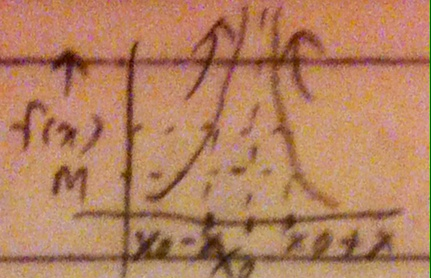
\includegraphics[scale=0.4]{infiniteLimitxo}
	\caption{\textgreek{Μη πεπερασμένο όριο στο} $x_0 \in \mathbb{R}$}
	\label{fig:infiniteLimitxo}
	\end{figure}
	
	\textgreek{Έστω} $f$ \textgreek{ορισμένη σε σύνολο της μορφής} $\displaystyle (\alpha,x_0) \cup (x_0, \beta)$. \textgreek{Ορίζουμε}:  
	\begin{itemize}
		\renewcommand{\labelitemi}{$\rightarrow$}
		\item $\displaystyle \lim_{x\to x_0} f(x) = +\infty$, \textgreek{όταν} $\forall M \in \mathbb{R}^+$ \textgreek{υπάρχει} $\delta > 0$ \textgreek{τέτοιο, ώστε} $\displaystyle  \forall x \in (\alpha,x_0) \cup (x_0, \beta)$ \textgreek{με} $0<|x-x_0| < \delta $ \textgreek{να ισχύει}: $f(x) > M$. 
		\item $\displaystyle \lim_{x\to x_0} f(x) = -\infty$, \textgreek{όταν} $\forall M \in \mathbb{R}^+$ \textgreek{υπάρχει} $\delta > 0$ \textgreek{τέτοιο, ώστε} $\displaystyle  \forall x \in (\alpha,x_0) \cup (x_0, \beta)$ \textgreek{με} $0<|x-x_0| < \delta $ \textgreek{να ισχύει}: $f(x) < -M$. 
	\end{itemize}
	\textbullet \quad If $\displaystyle P(x) = a_{\nu}x^{\nu} + a_{\nu-1} x^{\nu -1} + \ldots + a_0 $  :  polynomial equation, \textgreek{με} $a_{\nu} \neq 0$ \textgreek{ισχύει}: $\displaystyle \lim_{x\to +\infty} P(x) = \lim_{x\to + \infty} (a_{\nu} x^{\nu}) \land \lim_{x\to -\infty} P(x) = \lim_{x_{x\to -\infty}} (a_{nu} x^{\nu}) $ \linebreak 
	\textbullet \quad If $\displaystyle f(x) = \frac{a_{\nu}x^{\nu} + a_{\nu -1}x^{\nu -1} +\ldots + a_1x + a_0}{\beta_{\kappa}x^{\kappa} + \beta_{\kappa -1}x^{\kappa-1} + \ldots + \beta_1 x + \beta_0} $, $a_{\nu} \neq 0, \ \beta_{\kappa} \neq 0$, then: $\displaystyle \lim_{x\to +\infty} f(x) = \lim_{x\to +\infty} \left(\frac{a_{\nu}x^{\nu}}{\beta_{\kappa}x^{\kappa}}\right) \land \lim_{x\to -\infty} f(x) = \lim_{x\to -\infty} \left(\frac{a_{\nu}x^{\nu}}{\beta_{\kappa}x^{\kappa}}\right)$ \linebreak 
	\textbullet \quad $\displaystyle \alpha > 1 \rightarrow \left( \lim_{x\to -\infty} a^x = 0 \land \lim_{x\to \infty} a^x = + \infty \right) $ \linebreak 
	\textbullet \quad $\displaystyle \alpha > 1 \rightarrow \left( \lim_{x\to 0} \log_{\alpha} x = -\infty \land \lim_{x\to +\infty} log_{\alpha} x = -\infty \right) $ \linebreak 
	\textbullet \quad A sequence is every real function $\displaystyle \alpha: \mathbb{N}^* \rightarrow \mathbb{R}$. \textgreek{Θα λέμε ότι η ακολουθία} $\alpha_{\nu}$ \textgreek{έχει όριο το} $L\in \mathbb{R}$ \textgreek{και θα γράφουμε} $\displaystyle \lim_{\nu \to +\infty} \alpha_{\nu} = L$, \textgreek{όταν} $\displaystyle \forall \epsilon > 0, \exists \nu_0 \in \mathbb{N}^*$ \textgreek{τέτοιο, ώστε} $\displaystyle \forall \nu > \nu_0$ \textgreek{να  ισχύει}: $| \alpha_{\nu} - L | < \epsilon$ \linebreak 
	
	\textbullet \quad \uline{Discontinuity classification}:  
	\begin{enumerate}
	\item Removable discontinuity: has a "hole" in its graph, a term in the denominator that cancels out, 
	\item Non-Removable discontinuity: Has a "jump" at a point.
	\end{enumerate}
	\textbullet \quad $f$ is \uline{continuous} at $x_0 \in \Dom(f)$, iff $\displaystyle \lim_{x\to x_0} f(x) = f(x_0)$ \linebreak 
	\textbullet \quad \textgreek{Αν} $f,g$ \textgreek{συνεχείς στο} $x_0$, \textgreek{τότε είναι συνεχείς στο} $x_0$ \textgreek{και οι συναρτήσεις} $\displaystyle f+g, c\cdot f, c\in \mathbb{R}, f\cdot g, f/g, |f|, \sqrt[\nu]{f}$, \textgreek{με την προυπόθεση ότι ορίζονται σ'ένα διάστημα που περιέχει το} $x_0$. \linebreak 
	\textbullet \quad If $f$ is continuous at $x_0$ and $g$ continuous at $f(x_0)$, then their composition $g\circ f$ is continuous at $x_0$. \linebreak 
	\textbullet \quad $f$ \textgreek{είναι συνεχής σ'ενα ανοικτό διάστημα} $(a,b)$, \textgreek{όταν είναι συνεχής σε κάθε σημείο του} $(a,b)$. \linebreak 
	\textbullet \quad $f$ \textgreek{είναι συνεχής σ'ένα κλειστό διάστημα} $[a,b]$, \textgreek{όταν είναι συνεχής σε κάθε σημείο του} $(a,b)$ \textgreek{και επιπλέον} $\displaystyle \lim_{x\to \alpha^+} f(x) = f(\alpha) \quad \land \lim_{x\to \beta^-} f(x) = f(b)$. \linebreak 
	
	\textbullet \quad \uline{\textgreek{Θεώρημα} Bolzano}: \textgreek{Έστω μια συνάρτηση} $f$ \textgreek{, ορισμένη σε ένα κλειστό διάστημα} $[a,b]$. \textgreek{Αν}:
	\begin{itemize}
			\renewcommand{\labelitemi}{$\rightarrow$}
	\item \textgreek{η} $f$ \textgreek{είναι συνεχής στο} $[a,b]$ \textgreek{και επιπλέον, ισχύει} 
	\item $f(a) \cdot f(b) < 0$
	\end{itemize}
	\textgreek{τότε υπάρχει ένα, τουλάχιστον,} $x_0 \in (a,b)$ \textgreek{τέτοιο, ώστε} $f(x_0) = 0$, \textgreek{στο ανοικτό διάστημα} $(a,b)$. \linebreak 
	\textbullet \quad \textgreek{\uline{Θεώρημα Μέγιστης και Ελάχιστης τιμής}: Αν} $f$ \textgreek{συνεχής  στο} $[a,b]$, \textgreek{τότε η} $f$ \textgreek{παίρνει στο} $[a,b]$ \textgreek{μια μέγιστη τιμή} $M$ \textgreek{και μια ελάχιστη τιμή} $m$. \linebreak 
	\textbullet \quad \textgreek{Αν} $f$ \textgreek{γνησίως αύξουσα και συνεχής στο} $(a,b)$, \textgreek{τότε το σύνολο τιμών της στο διάστημα αυτό είναι το} $(A,B)$, \textgreek{όπου}: $\displaystyle A = \lim_{x\to a^+} f(x)$ \textgreek{και} $\displaystyle B= \lim_{x\to b^-} f(x)$. \linebreak \textgreek{Αν, όμως η} $f$ \textgreek{είναι γνησίως φθίνουσα και συνεχής στο} $(a,b)$, \textgreek{τότε το σύνολο τιμών της στο διάστημα αυτό είναι το} $(B,A)$. \linebreak 
	\textbullet \quad \textgreek{Έστω} $f$ \textgreek{και} $A(x_0, f(x_0))$ \textgreek{ένα σημείο της}. $\displaystyle \exists \lim_{x\to x_0} \frac{f(x)-f(x_0)}{x-x_0} \in \mathbb{R} \rightarrow$ \textgreek{εφαπτομένη (κλίση) της} $f$ \textgreek{στο Α είναι η ευθεία ε που διέρχεται από το Α και έχει συντελεστή διέυθυνσης λ}. \linebreak 
	\textbullet \quad $f$ is differentiable at point $x_0 \in \Dom(f)$, iff $\displaystyle \exists \lim_{x\to x_0} \frac{f(x)-f(x_0))}{x-x_0} \in \mathbb{R}$. This limit is the derivative of $f @ x_0$ and we denote it as $f'(x_0)$. Thus, $\displaystyle f'(x_0) = \lim_{x\to x_0} \frac{f(x)-f(x_0)}{x-x_0} $ \linebreak 
	\textbullet \quad Line $\displaystyle \epsilon: y -f(x_0) = f'(x_0) (x-x_0)$ \linebreak 
	\textbullet \quad If function $f$ is differentiable $@ a_0$, then it is also continuous $@ x_0$. \linebreak 
	\textbullet \quad \uline{\textgreek{Θεώρημα} Rolle}: \textgreek{Αν μια συνάρτηση} $f$ \textgreek{είναι}:  
	\begin{enumerate}
	\item \textgreek{συνεχής στο} $[a,b]$, 
	\item \textgreek{παραγωγίσιμη στο} $(a,b)$ \textgreek{και} 
	\item \textgreek{ισχύει ότι}: $f(a) = f(b)$,
	\end{enumerate}
	\textgreek{τότε υπάρχει ένα, τουλάχιστον} $x_0 \in (a,b)$ \textgreek{τ.ω.}: $f'(\xi)=0$. \linebreak 
	\textbullet \quad \uline{\textgreek{Θεώρημα Μέσης Τιμής (Θ.Μ.Τ.)}}: \textgreek{Έστω συνάρτηση} $f$. \textgreek{Αν}  
	\begin{enumerate}
	\item $f$ \textgreek{συνεχής στο} $[a,b]$, 
	\item $f$ \textgreek{παραγωγίσιμη στο} $(a,b)$, 
	\end{enumerate}
	\textgreek{τότε υπάρχει ένα, τουλάχιστον} $x_0 \in (a,b)$ \textgreek{τ.ω.}: $\displaystyle f'(x_0) = \frac{f(b)-f(a)}{b-a}$  :  \textgreek{που είναι ο μέσος ρυθμός μεταβολής της} $f$ \textgreek{στο} $(a,b)$. \linebreak 
	
	Suppose function $f$, continuous among space $\Delta = (a,b)$. \linebreak 
	\textbullet \quad $\displaystyle \forall x \in \Delta \left( f'(x) > 0 \right) \rightarrow f \uparrow \Delta$ \linebreak 
	\textbullet \quad $\displaystyle \forall x \in \Delta \left( f'(x) < 0 \right) \rightarrow f\downarrow \Delta$ \linebreak 
	\textbullet \quad \uline{\textgreek{Θεώρημα} Fermat}: If $f$ has a stationary point at $\displaystyle x_0 \in \Delta \subset \Dom(f)$ and $f$ is differentiable at that point, then $f'(x_0) = 0$. \linebreak 
	
	Stationary points \linebreak 
	\textbullet \quad Let $\displaystyle x_0 \in \Delta, \ (f'(x_0) = 0 \land f''(x_0) < 0) \rightarrow f(x_0)$ local maximum. \linebreak 
	\textbullet \quad Let $\displaystyle x_0 \in \Delta.\ (f'(x_0) = 0 \land f''(x_0) > 0 ) \rightarrow f(x_0)$ local minimum. \linebreak 
	\textbullet \quad \uline{Determining Points of Inflexion (POI)}: Let $\displaystyle x_0 \in \Delta \subset \Dom(f)$  
	\begin{enumerate}
	\item We differentiate $\displaystyle y=f(x)$ twice to get $\frac{d^2 y}{dx^2}$. 
	\item We solve the equation $\displaystyle \frac{d^2y}{dx^2}= 0$.
	\item We test to see whether, or not a change of sign occurs in $\displaystyle \frac{d^2y}{dx^2}$, at $x=x_0+a$ and at$x=x_0 -a$. If $f(x_0 + a) \cdot f''(x_0-a) < 0 \rightarrow x_0$  :  P.O.I. 
	\end{enumerate}
		\textbullet \quad $\displaystyle \forall x\in \Delta (\frac{d^2y}{dx^2} > 0) \rightarrow f$ convex / concave-upwards $\displaystyle @ \Delta \quad (\cup shape)$ \linebreak 
	\textbullet \quad $\displaystyle \forall x\in \Delta (\frac{d^2y}{dx^2} < 0) \rightarrow f$ convex / concave-downwards $\displaystyle @ \Delta \quad (\cap shape)$ \linebreak 
	\textbullet \quad $\displaystyle \frac{df(x)}{dx} = $ undefined for some $x=x_0$, then $\left(x_0, f(x_0)\right)$ is a critical point. \linebreak 
	\textbullet \quad $(\displaystyle f+g)'(x_0) = f'(x_0) + g'(x_0)$ \linebreak 
	\textbullet \quad $\displaystyle f\cdot g)'(x_0) = f'(x_0) g(x_0) + f(x_0) g'(x_0)$ \linebreak 
	\textbullet \quad $\displaystyle (\frac{f}{g})'(x_0) = \frac{f'(x_0)g(x_0) -f(x_0)g'(x_0)}{[g(x_0)]^2} $ \linebreak 
	\textbullet \quad \uline{Chain rule}: $\displaystyle f'(g(x_0)) = (f \circ g)'(x_0) = f'(g(x_0)) \cdot g'(x_0) $ \textgreek{ή} $\displaystyle \frac{dy}{dx} = \frac{dy}{dz} \cdot \frac{dz}{dx} $ \linebreak 
	
	\textbullet \quad Differerentiation of parametric equations: $x=f(t), y=g(t)$ we find: $\displaystyle \frac{dx}{dt}\ , \ \frac{dy}{dt}$ and finally we evaluate: $\displaystyle \frac{dy}{dx} = \frac{dy}{dt} \cdot \frac{dt}{dx} $ \linebreak 
	\textbullet \quad Curvature of a curve at a point $P$. It tells us how quickly the curve is bending in the immediate neighborhood of that point $P$. \linebreak 
	\textbullet \quad Radius of curvature: $\displaystyle R=\frac{\big[ 1 + \left( \frac{dy}{dx} \right)^2 \big]^{\frac{3}{2}}}{\frac{d^2y}{dx^2}} $ ($R$ is large $\rightarrow$ curvature is small) \linebreak 
	\textbullet \quad Centre of curvature $(h,k)$, of the circle at point $\displaystyle P(x_1, y_1)$  :  $h = x_1 - R\sin \theta \ \land \ k = y_1 + R \cos \theta $ \linebreak 
	
	\textbullet \quad \uline{Indeterminate Forms}: are algebraic expressions obtained in the context of limits. Limits involving algebraic operations are often performed by replacing subexpressions by their limits; if the expression obtained after this substitution does not give enough information to determine the original limit, it is known as an indeterminate form. Indeterminate forms: \linebreak 
	 $\displaystyle \frac{0}{0}\ , \frac{\infty}{\infty}\ , \ \infty - \infty , 0 \cdot \infty , 1^{\infty} \ , \ 0^0\ , \ \infty^0 \ , \ e^{\pm j \infty} $ \linebreak 
	\textbullet \quad \uline{L'Hospital's rule} for circumventing indeterminate forms: We take the derivatives of both the numerator and the denominator. \linebreak 
	
	\textbullet \quad \uline{Asymptotes}: first express the equation "on one line". \linebreak 
	\textbullet \quad Asymptotes parallel to the $x$-axis: We equate the coefficient of the highest power of $x$ to zero. \linebreak 
	\textbullet \quad Asymptotes paralle to the $y$-axis: We equate the coefficient of the highest power of $y$ to zero. \linebreak 
	\textbullet \quad Other asymptotes: To find a (general type) asymptote to $y=f(x)$  :   
	\begin{enumerate}
	\item Substitute $y=mx + c$ in the given equation and simplify. 
	\item Equate to zero the coefficients of the two highest powers of $x$ and so determine the values of $m \land c$. \linebreak 
	\end{enumerate}

	\uline{Symmetry}: \linebreak 
	\textbullet \quad If only even powers of $y \ (x) $ occur the curve is symmetrical about the $x \ (y)$ axis. \linebreak 
	
	\uline{Limitations} \linebreak 
	\textbullet \quad First, always check for restrictions on the possible range of values that $x$, or $y$ may have. \linebreak 
	\textbullet \quad Symmetry about origin: replace both $x$ with $-x$ and $y$ with $-y$. If it's the same equation then it is symmetric. \linebreak 
	\textbullet \quad Symmetric about $x$-axis: replace $x$ with $-x$. Check. \linebreak 
	\textbullet \quad Symmetric about $y$-axis: replace $y$ with $-y$. Check. \linebreak 
	
	\textbullet \quad Differentials $dy, dx$ are finite quantities -not necessarily zero- and can therefore exist alone. $dy = f'(x_0)\ dx$ \linebreak 
	\textbullet \quad Root Mean Square \uline{(R.M.S.)} value of a function: $\displaystyle y=f(x) \ , \ \overset{~}{y} = \sqrt{\frac{1}{b-a} \int_a^b y^2 dx} $ \linebreak 
	\textbullet \quad The \uline{General Leibniz rule} generalizes the product rule. It states that if $f$ and $g$ are $n$-times differentiable functions, then the product $fg$ is also $n$-times differentiable and its $n$th derivative is given by: \linebreak 
	$\displaystyle \left( fg \right)^{(n)} (x) = \sum \limits_{k=0}^n \binom{n}{k} f^{(n-k)} (x) g^{(k)} (x) $ \linebreak 
	This can be proved by using the product rule and mathematical induction. \linebreak 
	
	\subsubsection{Derivatives}
		
	\textbullet \quad $\displaystyle f(x) = C \rightarrow f'(x) = 0 $ \linebreak 
	\textbullet \quad $\displaystyle f(x) = x^k, k \in \mathbb{R} \rightarrow f'(x) = kx^{k-1} $ \linebreak 
	\textbullet \quad $\displaystyle f(x) = \sqrt{x}, x\geq 0 \rightarrow f'(x) = (1/2) \cdot x^{\frac{-1}{2}}, \ x> 0 $ \linebreak 
	\textbullet \quad $\displaystyle f(x) = \sin (x) \rightarrow f'(x) = \cos (x) $ \linebreak 
	\textbullet \quad $\displaystyle f(x) = \cos (x) \rightarrow f'(x) = -\sin (x)$ \linebreak 
	\textbullet \quad $\displaystyle f(x) = e^x \rightarrow f'(x) = e^x $ \linebreak 
	\textbullet \quad $\displaystyle f(x) = \ln(x), \ x> 0 \rightarrow f'(x) = \frac{1}{x} $ \linebreak 
	\textbullet \quad $\displaystyle f(x) = \log_a(x) \rightarrow f'(x) = \frac{1}{xln(a)} $ \linebreak 
	\textbullet \quad $\displaystyle f(x) = \tan (x) , x\neq \pi / 2 \rightarrow f'(x) = \sec ^2 (x) $ \linebreak 
	\textbullet \quad $\displaystyle f(x) = \cot (x), x\neq 0 \rightarrow f'(x) = -\cosec ^2(x) $ \linebreak 
	\textbullet \quad $\displaystyle f(x) = x^{-k}, k \in \mathbb{R}, x\neq 0 \rightarrow f'(x) = -kx^{-k-1} $ \linebreak 
	\textbullet \quad $\displaystyle f(x) = a^x, a> 0 \rightarrow f'(x) = a^x lna $ \linebreak 
	\textbullet \quad $\displaystyle f(x) = \arcsin (x) = \sin ^{-1}(x) \rightarrow f'(x) = \frac{1}{\sqrt{1-x^2}} $ \linebreak 
	\textbullet \quad $\displaystyle f(x) = \cos ^{-1} (x) \rightarrow f'(x) = \frac{-1}{sqrt{1-x^2}} $ \linebreak 
	\textbullet \quad $\displaystyle f(x) = \tan^{-1}(x) \rightarrow f'(x) = \frac{1}{1+x^2} $ \linebreak 
	\textbullet \quad $\displaystyle f(x) = \cot ^{-1} (x) \rightarrow f'(x) = \frac{-1}{1+x^2} $ \linebreak 
	\textbullet \quad $\displaystyle f(x) = \sinh (x) \rightarrow f'(x) = \cosh (x) $ \linebreak 
	\textbullet \quad $\displaystyle f(x) = \cosh (x) \rightarrow f'(x) = \sinh (x) $ \linebreak 
	\textbullet \quad $\displaystyle f(x) = \tanh (x) \rightarrow f'(x) = 1-\tanh ^2(x) $ \linebreak 
	\textbullet \quad $\displaystyle f(x) = \coth(x) \rightarrow f'(x) = 1-\coth ^2(x) $ \linebreak 
	\textbullet \quad $\displaystyle f(x) = \sinh ^{-1} (x) \rightarrow f'(x) = \frac{1}{\sqrt{1+x^2}} $ \linebreak 
	\textbullet \quad $\displaystyle f(x) = \cosh ^{-1} (x) \rightarrow f'(x) = \frac{1}{\sqrt{x^2 -1}} $ \linebreak 
	\textbullet \quad $\displaystyle f(x) = \tanh ^{-1} (x) \rightarrow f'(x) = \frac{1}{1-x^2} $ \linebreak 
	\textbullet \quad $\displaystyle f(x) = \coth ^{-1} (x) \rightarrow f'(x) = \frac{1}{1+x^2} $ \linebreak 
	\textbullet \quad $\displaystyle f(x) = g^k(x) \rightarrow f'(x) = k g^{k-1}(x) g'(x)$ \linebreak 
	\textbullet \quad $\displaystyle f(x) = \sqrt{g(x)}, g(x) \geq 0 \rightarrow f'(x) = \frac{1}{2\sqrt{g(x)}} g'(x), \ g(x) > 0 $ \linebreak 
	\textbullet \quad $\displaystyle f(x) = \sin (g(x)) \rightarrow f'(x) = g'(x) \cos (g(x)) $ \linebreak 
	\textbullet \quad $\displaystyle f(x) = e^{g(x)} \rightarrow f'(x) = e^{g(x)} \cdot g'(x) $ \linebreak 
	\textbullet \quad $\displaystyle f(x) = x^x \rightarrow f'(x) = x^x \cdot (1 + \ln x) $ \linebreak 
	\textbullet \quad $\displaystyle f(x) = \ln (g(x)) \rightarrow f'(x) = (\frac{1}{g(x)} \cdot g'(x)$ \linebreak 
	\textbullet \quad $\displaystyle f(x) = \tan (g(x)) \rightarrow f'(x) = \frac{1}{\cos ^2(g(x))} g'(x) $ \linebreak 
	\textbullet \quad $\displaystyle f(x) = u(x)^{g(x)} \rightarrow f'(x) = \left( e^{g(x) \cdot \ln (u(x))} \right)' $ \linebreak 
	\textbullet \quad $\displaystyle f(x) = \frac{1}{g(x)}, g(x) \neq 0 \rightarrow f'(x) = \frac{-1}{g^2(x)} g'(x) $ \linebreak 
	\textbullet \quad $\displaystyle f(x) = \log_a(g(x)) \rightarrow f'(x) = \frac{1}{\ln (a) g(x)} g'(x)$ \linebreak 
	\textbullet \quad $\displaystyle f(x) = \sec (x) \rightarrow f'(x) = \tan (x) \cdot \sec (x) $ \linebreak 
	\textbullet \quad $\displaystyle f(x) = \sin (ax) \rightarrow f^{(n)}(x) = a^n \cdot \sin (ax + \frac{n\pi}{2} $ \linebreak 
	\textbullet \quad $\displaystyle f(x) = \cos (ax) \rightarrow f^{(n)}(x) = a^n \cdot \cos (ax + \frac{n\pi}{2} $ \linebreak 
	\textbullet \quad $\displaystyle f(x) = e^{ax} \rightarrow f^{(n)}(x) = a^n e^{ax} $ \linebreak 
	\textbullet \quad $\displaystyle f(x) = \ln(x) \rightarrow f^{(n)}(x) = \frac{\left[ (-1)^{n-1} (n-1)! \right]}{x^n} $ \linebreak 
	\textbullet \quad $\displaystyle f(x) = \sinh (ax) \rightarrow f^{(n)}(x) = \frac{a^n}{2} \cdot \{ [1+(-1)^n] \sinh (ax) + [1-(-1)^n] \cdot \cosh (ax) \}$ \linebreak 
	\textbullet \quad $\displaystyle f(x) = \cosh (ax) \rightarrow f^{(n)}(x) = \frac{a^n}{2} \cdot \{[1+(-1)^n] \cosh (ax) +[1-(-1)^n] \cdot \sinh (ax) \} $ \linebreak 
	\textbullet \quad $\displaystyle f(x) = x^a, a> 0 \rightarrow f^{(n)} (x) = \frac{a!}{(a-n)!} x^{a-n} $ \linebreak 
	
	\subsubsection{Numerical solutions to Derivatives} 
	
	\uline{Numerical Solutions to Derivatives of $f(x)$} \linebreak 
	\textbullet \quad Forward difference formula: $\displaystyle f'(x) \approx \frac{f(x+h)-f(x)}{h}$ \linebreak 
	(neglecting terms of order $2$ and above) 
	\textbullet \quad Backward difference formula: $\displaystyle f'(x) \approx \frac{f(x) - f(x-h)}{h}$ \linebreak 
	(neglecting terms of order $2$ and above) 
	\textbullet \quad Central difference formulas: (more accurate) (neglecting terms of order $3$ and above) \linebreak 
	$\displaystyle f'(x) \approx \frac{f(x+h) - f(x-h)}{2h} $ \linebreak 
	$\displaystyle f''(x) \approx \frac{f(x+h) -2f(x) + f(x-h)}{h^2} $ \linebreak 
	
	\subsubsection{Partial Differentiation}	
	
	\textbullet \quad Notation: $\displaystyle f_x(x,y) = \frac{\partial}{\partial x} f(x,y) \ , \ f_{xx} (x,y) = \frac{\partial^2}{\partial x^2} f(x,y) \ , \ f_{yx} (x,y) = \frac{\partial^2}{\partial y \cdot \partial x} f(x,y)$ \linebreak 
	\textbullet \quad Partial differentiation with respect to a given variable, say $x$  :  We are certain that all other variables, besides $x$, are held constant for the time being. \linebreak 
	\textbullet \quad Taylor's theorem for two independent variables: $\displaystyle f(x+h, y+k) = f(x,y) + \{ hf_x (x,y) + kf_y (x,y) \} + \frac{1}{2!} \{ h^2 f_{xx} (x,y) + 2hkf_{xy} (x,y) + k^2 f_{yy} (x,y) \} + \frac{1}{2!} \{ kh^2 f_{yxx} (x,y) + k^2 h f_{yyx} (x,y) \} + \ldots $ \linebreak 
	\textbullet \quad A function $f(x)$ is an \uline{infinitesimal} at $x_0$, if its limit at $x_0$ is zero, e.g. $\lim_{x\to 0} \sin (x) = 0 \ \ \therefore x_0 = 0$ \linebreak 
	
	\textbullet \quad \uline{Function's Differential}: Suppose $\displaystyle z=f(x,y,w,\ldots , n)$ , where $x,y,w, \ldots, n$ are the independent variables of $f$. A function's differential shows its functions behaviour for small changes in all of its independent variables. With satisfying accuracy it's approximated to be: \linebreak 
	$\displaystyle \delta z = \frac{\partial z}{\partial x} \delta x + \frac{\partial z}{\partial y} \delta y + \frac{\partial z}{\partial x} \delta w + \ldots + \frac{\partial z}{\partial n} \delta n $ (+ higher order derivatives of $x,y,w,\ldots , n$ of smaller magnitude / value) \linebreak 
	\textbullet \quad \uline{Rates of change}: If $z = f(x,y)$, then if $z$ changes with respect to $\delta t$ and $\delta t \rightarrow 0$ then \linebreak 
	$\displaystyle \frac{\delta z}{\delta t} = \frac{\partial z}{\partial x} \cdot \frac{\partial x}{\partial t} + \frac{\partial z}{\partial y} \cdot \frac{\delta y}{\delta t} $ \linebreak 
	\textbullet \quad Parametric functions: If $z=f(x,y)$ and $x=g(u,v) \ , y=h(u,v)$ then $z=k(u,v)$. To find $\displaystyle \frac{\partial z}{\partial u}$ and $\frac{\partial z}{\partial y}$ we do: \linebreak 
	$$ \frac{\partial z}{\partial u} = \frac{\partial z}{\partial x} \cdot \frac{\partial x}{\partial u} + \frac{\partial z}{\partial y} \cdot \frac{\partial y}{\partial u} \ \land \ \frac{\partial z}{\partial v} = \frac{\partial z}{\partial x} \cdot \frac{\partial x}{\partial	v} + \frac{\partial z}{\partial y} \cdot \frac{\partial y}{\partial v} $$ 
	\textbullet \quad Implicit functions: If $f(x,y) = 0$ is an implicit function, we let $z=f(x,y)$. Then: $\displaystyle  \frac{dy}{dx} = - \big( \frac{\partial z}{\partial x} / \frac{\partial z}{\partial y} \big) $ \linebreak 
	\textbullet \quad $\displaystyle z= f(x,y) \rightarrow \frac{\partial^2 z}{\partial x \partial y} = \frac{\partial^2 z}{\partial y \partial x} = \frac{\partial}{\partial x} \big( \frac{\partial z}{\partial y} \big) = \frac{\partial}{\partial y} \big( \frac{\partial z}{\partial x} \big) $ \linebreak 
	\textbullet \quad Inverse functions and Jacobian usage: \linebreak 
	If $z=f(x,y)$ and $u=g(x,y)$ and $v=h(x,y)$ then: \linebreak 
	$$ \frac{\partial x}{\partial u} = \frac{\partial v}{\partial y} / J \ , \ \frac{\partial x}{\partial v} = - \frac{\partial u}{\partial y} / J \ , \ \frac{\partial y}{\partial u} = - \frac{\partial v}{\partial x} / J \ , \ \frac{\partial y}{\partial v} = \frac{\partial u}{\partial x} / J $$ 
	% inline matrix with \begin{smallmatrix}
	where the Jacobian of $u, v$ with respect to $x,y$ is: \linebreak 
	$$ \displaystyle J(x,y) = \frac{\partial(u,v)}{\partial(x,y)} = \left[ \begin{smallmatrix} \frac{\partial u}{\partial x} & \frac{\partial v}{\partial x} \\ \frac{\partial u}{\partial y} & \frac{\partial v}{\partial y} \end{smallmatrix} \right]$$ \linebreak 
	\textbullet \quad Inverse Jacobian: $\displaystyle \mathbb{J}(x,y)^{-1} = \mathbb{J}(u,v) = \frac{\partial (x,y)}{\partial (u,v)} = \frac{1}{\frac{\partial (u,v)}{\partial (x,y)}} = 1 \div \begin{smallmatrix} \frac{\partial x}{\partial u} & \frac{\partial y}{\partial u} \\ \frac{\partial x}{\partial v} & \frac{\partial y}{\partial v} \end{smallmatrix} $ \linebreak 
	
	\textbullet \quad \uline{Stationary points of functions in 3 dimensions} \linebreak 
	i.e. $z=f(x,y)$. Four steps in the routine:  
	\begin{enumerate}
	\item Find $\displaystyle \frac{\partial z}{\partial x}$ and $\displaystyle \frac{\partial z}{\partial y}$ and solve $\displaystyle \frac{\partial z}{\partial x} = 0$ and $\displaystyle \frac{\partial z}{\partial y} = 0$. If found any, then $(x_0,y_0)$ is a stationary point. 
	\item If $\displaystyle \big( \frac{\partial^2 z}{\partial x^2} \big) \cdot \big( \frac{\partial^2 z}{\partial y^2} \big) - \big( \frac{\partial^z}{\partial x \partial y} \big) > 0 \ @ \ (x_0, y_0)$, then the point $(x_0, y_0)$ is either a maximum, or a minimum (over $(x_0 + h, y_0 + k)$ in any direction from the point). 
	\item If $\frac{\partial^2 z}{\partial x^2}$ and $\frac{\partial^2 z}{\partial y^2}$ are both negative then $(x_0, y_0)$ is a maximum. If $\frac{\partial^2 z}{\partial x^2}$ and $\frac{\partial^2 z}{\partial y^2}$ are both positive then $(x_0,y_0)$ is a minimum. 
	\item We evaluate the actual minimum, or maximum values, i.e. we find $f(x_0, y_0)$. 
	\end{enumerate}
	
	\textbullet \quad If $\displaystyle \big( \frac{\partial^2 z}{\partial x^2} \big) \cdot \big( \frac{\partial^2 z}{\partial y^2} \big) - \big( \frac{\partial^2 z}{\partial x \partial y} \big)^2 < 0$, then further, detailed study (most likely) is necessary to determine the stationary points. \linebreak 
	\textbullet \quad \uline{Lagrange multipliers}: Used to find extremal values of a function $u= f(x,y,z,\ldots)$, with constraint $\phi (x,y,z,\ldots) = 0$. Then we need to find these $x,y,z,\ldots$ points in order to calculate the extremal value $u= f(x,y,z,\ldots)$. For this purpose we solve a system of equations whose number is the one of the unknown variables $+1$ (for the constraint equation). If $u=f(x,y,z)$, with constraint $\phi (x,y,z)=0$, then we solve the following system of 4 equations: \linebreak 
	$$ \frac{\partial u}{\partial x} + \lambda \frac{\partial \phi}{\partial x} = 0 {\text{\tiny (I)}} \ , \frac{\partial u}{\partial y} + \lambda \frac{\partial \phi}{\partial y} = 0 {\text{\tiny (II)}} \ , \ \frac{\partial u}{\partial z} + \lambda \frac{\partial \phi}{\partial z} = 0 {\text{\tiny (III)}} \ , \ \phi(x,y,z) = 0 {\text{\tiny (IV)}} $$ \linebreak 
	
	\textbullet \quad Any expression $\displaystyle dz = Pdx + Qdy \ , \ P = f(x) \ , \ Q = g(y)$ is an \uline{exact differential} if it can be integrated to determine $z$. Therefore if $\displaystyle \frac{\partial^2 z}{\partial y \partial x} = \frac{\partial^2 z}{\partial x\partial y}$, then $dz$ is an exact differential. The concept can be extended to functions of more than two variables. \linebreak 
	\textbullet \quad Exact differential in $3$ independent variables. \linebreak 
	$\displaystyle dw = P dx + Q dy + R dz$ is an exact differential of $\displaystyle w= f(x,y,z)$ , if $\displaystyle \frac{\partial P}{\partial y} = \frac{\partial Q}{\partial x} \land \frac{\partial P}{\partial z} = \frac{\partial R}{\partial x} \land \frac{\partial Q}{\partial z} = \frac{\partial R}{\partial y}$ \linebreak 	
	
	\subsection{Integral Calculus}
	
	\textbullet \quad \textgreek{Αρχική συνάρτηση, ή παράγουσα της} $f$ \textgreek{στο} $\Delta$ \textgreek{ονομάζεται κάθε συνάρτηση} $F$ \textgreek{που είναι παραγωγίσιμη στο} $\Delta$ \textgreek{και ισχύει}: $\displaystyle F'(x) = f(x),\ \forall x\in \Delta$. \linebreak 
	\textbullet \quad \textgreek{Αν} $F$ \textgreek{παράγουσα της} $f$ \textgreek{στο} $\Delta$, \textgreek{τότε όλες οι συναρτήσεις της μορφής} $\displaystyle G(x) = F(x) + c, \ c\in \mathbb{R}$ \textgreek{είναι παράγουσες της} $f$ \textgreek{στο} $\Delta$. \linebreak 
	\textbullet \quad \textgreek{Το σύνολο όλων των παραγουσών της} $f$ \textgreek{στο} $\Delta$ \textgreek{ονομάζεται αόριστο ολοκλήρωμα της} $f$ \textgreek{στο} $\Delta$. \linebreak 
	\textbullet \quad \uline{Fundamental Theorem of Calculus}: If $f$ is continuous in $[a,b]$, then it has an antiderivative: $\displaystyle F(x) = \int_a^x f(t) dt, \ x\in [a,b]$. \linebreak $\displaystyle \therefore \frac{dF}{dx} = \frac{d}{dx} \int_a^x f(t) dt = f(x)$. Corrolary: $\int_a^b f(t) dt = F(b) - F(a)$, i.e. $f$ is Riemann integrable on $[a,b]$. \linebreak 
	\textbullet \quad $\displaystyle \int f(x) g'(x) dx = f(x) g(x) - \int f'(x) g(x) dx$  :  Integration by parts\linebreak 
	\textbullet \quad $\displaystyle \int f(g(x)) g'(x) dx = \int f(u) du$  :  Integration by substitution \linebreak 
	\qquad $\displaystyle u= g(x) \ land du = g'(x) dx$ \linebreak 
	\textbullet \quad $\displaystyle \int \frac{f'(x)}{f(x)} dx = \ln [f(x)] + C $ \linebreak 
	\textbullet \quad  $\displaystyle \int f(x) f'(x) dx = \frac{f^2(x)}{2} + C $ \qquad ($=\int zdz$) \linebreak 
	\qquad $\displaystyle z=f(x), \ dz= f'(x) dx$ \linebreak 
	\textbullet \quad To integrate a "function of a linear function of x", simply replace $x$ in the corresponding standard result by the linear expression and divide by the coefficient of $x$ in the linear expression. \linebreak 
	
	\textbullet \quad The total area $A$ between a curve $f(x) = y$ and the $x$ axis, from $x=a$ to $x=b$, is given by $\displaystyle  A = \int_a^b y \ dx$ \linebreak 
	\textbullet \quad Area between a curve and an intersecting line from $x=a$, to $x=b$ is: $\displaystyle A = \int_a^b (y_1 -y_2) dx $ \linebreak 
	\textbullet \quad The equation that is "more positive" (from $a$ to $b$) is $y_1$ (either the line of the curve) \linebreak 

	\textbullet \quad \uline{Partial Fractions}  
	\begin{enumerate}
	\item It is necessary that the degree of the numerator is less than the degree of the denominator. 
	\item In such an expression that the denominator can be expressed as a product of simple prime factors, each one of the $ax+b$  :  
		\begin{enumerate}
		\item Write the rational expression with the denominator given as product of its prime factors, 
		\item Each factor then gives rise to a partial fraction of the form: $\displaystyle \frac{A}{ax + b}$, where$A$ is a constant whose value is to be determined.
		\item Add the partial fractions together to form a single algebraic fraction whose numerator contains the unknown constants and whose denominator is identical to that of the original expression, 
		\item Equate the numerator so obtained with the numerator of the original algebraic fraction, 
		\item By substituting appropriate values of $x$ in this equationdetermine the values of the unknown constants. You'll have to solve a system of linear equations whose number is that of the unknown constants.
		\end{enumerate}	
	
	\item In such a case that the denominator of the original rational expressionn of the form $(ax^2 +bx +c)$ is irreducible, it gives rise to a partial fraction of the form: $\displaystyle \frac{Ax+b}{ax^2+bx+c}$ 
	\item In such a case that the denominator of the original rational expression contains algebraic repeated facors of the form $ax+b)^n$, these give rise to partial fractions of the form: $\displaystyle \frac{A_1}{ax+b} + \frac{A_2}{(ax+b)^2} + \ldots + \frac{A_n}{(ax+b)^n}, \quad n\in \mathbb{N}^*.$ \linebreak 
	\end{enumerate}
	
	\uline{Heavyside's Cover up Method} \linebreak 
	\textbullet \quad $\displaystyle y(x) = \frac{v(x)}{B(x-p_1)(x-p_2)\cdots(x-p_{\nu})} = \frac{k_1}{x-p_1} + \frac{k_2}{x-p_2} + \ldots + \frac{k_{\nu}}{x-p_{\nu}} $ \linebreak 
	\textbullet \quad \textgreek{Αν} $p_i$  :  \textgreek{απλός πόλος, τότε}: $k_i = \left[(x-p_i)y(x)\right]_{x=p_i}$
	\textbullet \quad \textgreek{Αν} $p_i$  :  \textgreek{πολλαπλός πόλος, πολλαπλότητας} $m$, \textgreek{δηλαδή} $\displaystyle \frac{\nu(x)}{(x-p_i)^m} = \frac{k_1}{x-p_i} + \frac{k_2}{(x-p_i)^2} + \ldots + \frac{k_m}{(x-p_i)^m} $, \textgreek{τότε}:  
	\begin{itemize}
		\renewcommand{\labelitemi}{$\rightarrow$}
	\item	$\displaystyle k_i= \frac{1}{(i-1)!} \cdot \frac{d^{i-1}}{dx^{i-1}} \left[(x-p_i)^m y(x) \right]_{x=p_i} \ , \ i=2,3,\ldots, m$ 
	\item $\displaystyle k_i = \left[ (x-p_i)^m y(x) \right]_{x=p_i} \ , \ i=m$, i.e. highest order repeated root.  
	\end{itemize}
	\textbullet \quad \textgreek{Αν} $p_i$  :  \textgreek{μιγαδικό ζεύγος πόλων, δλδ.}: \linebreak 
	$\displaystyle \frac{\nu(x)}{x-p_i} = \frac{k_1}{x-a-jb} + \frac{k_2}{x-a+jb} $, \textgreek{τότε} $k_1 = \overset{-}{k_2},\quad k_1, k_2 \in \mathbb{C} $ \linebreak 
	$\displaystyle k_1 = \left[ (x-a-jb) y(x) \right]_{x=a+jb} = \lim_{x\to a+jb} \left[(x-a-jb) y(x) \right] $ \linebreak 
	
	\textbullet \quad Mean value of a function $f$ between two limits $a$ and $b$  :  \linebreak 
	$\displaystyle M = \frac{\text{Area}}{b-a} = \frac{1}{b-a} \int_a^b y dx \qquad , \ b>a\ , \ y=f(x)$ \linebreak 
	\textbullet \quad \uline{\textgreek{Θ.Μ.Τ. ολοκληρωτικού λογισμού}}: \textgreek{Για} $f$ \textgreek{που ορίζεται στο} $(a,b) \subset \Dom (f)$ \textgreek{και έστω} $c \in (a,b)$. \textgreek{Τότε}: $\displaystyle F'(c) = \frac{F(b) - F(a)}{b-a} $ \linebreak 
	\textbullet \quad We get that: $\displaystyle \int_a^b f(x) dx = f(c) (b-a) $ and $\displaystyle f(c) = \frac{\int_a^b f(x) dx}{b-a} $ is the mean value of $f$ in the interval $(a,b)$. \linebreak 
	\textbullet \quad Integration as a summing process: \linebreak 
	when $\displaystyle \delta x \rightarrow 0 \: \ \sum \limits_{x=a}^{x=b} y \delta x = \int_a^b ydx$ \linebreak 
	
	\textbullet \quad Moment of mass of element about axis = $r \cdot \delta m $, $\ r$  :  distance from the axis.\linebreak 
	\textbullet \quad Volume of a solid of revolution rotating about the $x$-axis: $\displaystyle V= \int_a^b \pi y^2 dx$, when the function is given in parametric form then: $\displaystyle V=\int_a^b \pi y^2 \frac{dx}{dt} dt$ \linebreak 
	\textbullet \quad Volume of a solid of revolution rotating about the $y$-axis: $\displaystyle V = 2\int_a^b \pi xy dx$ \linebreak 
	\textbullet \quad Surface Area of plane figure: $A=\int_a^b ydx$ \linebreak 
	\textbullet \quad Centroid $\displaystyle \left( \overset{-}{x}, \overset{-}{y} \right)$ of plane figure: $\displaystyle \overset{-}{x} = \frac{1}{A} \int_A x_e dA = \frac{1}{A} \int_a^b xy dx$ and $ \overset{-}{y} = \frac{1}{A} \int_A y_e dA = \frac{1}{A} \int_a^b \frac{y}{2} ydx = \frac{1}{2A} \int_a^b y^2 dx$ \linebreak 
	\textbullet \quad Centre of gravity (or mass) of a solid of revolution, revolving about the x-axis: $\displaystyle \overset{-}{x} = \frac{\int_a^b xy^2 dx}{\int_a^b y^2 dx}$ and $\overset{-}{y} = 0$ \linebreak 
	\textbullet \quad Length of a curve: $\displaystyle S = \int_a^b \sqrt{1+\left( \frac{dy}{dx} \right)^2 } dx$, when the function is given in parametric form (i.e.$\displaystyle x=f(\partial), y=g(\partial)$  :  $\displaystyle A = 2\pi \int_a^b y \sqrt{\left(\frac{dx}{d\partial}\right)^2 + \left(\frac{dy}{d\partial}\right)^2} d\partial $ \linebreak 
	\textbullet \quad Centre of gravity of a solid of revolution that rotates about the y-axis: $\displaystyle \overset{-}{x} = 0$ and $\displaystyle \overset{-}{y} = \frac{\int_a^b yx^2 dy}{\int_a^b x^2 dy} $ \linebreak 
	\textbullet \quad Surface of revolution generated by the arc of a curve rotating about the y-axis: $\displaystyle A=2\pi \int_a^b x \sqrt{1 + \left( \frac{dy}{dx} \right)^2} dx $ \linebreak 
	\textbullet \quad \uline{1st rule of Pappus}: If an arc of a plane curve rotates about an axis in its plane, the area of the surface generated is equal to the length of the line multiplied by the distance travelled by its centroid. \linebreak 
	\textbullet \quad \uline{2nd rule of Pappus}: If a plane figure rotates about an axis in its plane, the volume generated is equal to the area of the figure multiplied by the distance travelled by its centroid.  
	\begin{itemize}
		\renewcommand{\labelitemi}{$\rightarrow$}
	\item One proviso / caveat in using the rules of Pappus: the axis of rotation must not cut the rotating arc, or plane figure. 
	\end{itemize}
	
	\textbullet \quad Whenever we have a problem not covered by our standard results, we build up the integral from first principles. \linebreak 
	\textbullet \quad $\displaystyle KE = \frac{1}{2} mU^2 = \frac{1}{2} m\omega^2 r^2 = \frac{1}{2} \omega^2 \sum mr^2 (J) $  :  Kinetic Energy \linebreak 
	\textbullet \quad \uline{Moment of Inertia} (\textgreek{ροπή αδράνειας}): $\displaystyle I = \sum mr^2 (\frac{kg}{m^2}) $  :  Physical property of the object. It's a sum for all of its particles, $r$  :  distance from axis of rotation. \linebreak 
	The M.O.I. is also called rotational mass, because it does the same thing in rotational dynamics as mass does in linear dynamics. \linebreak 
	\textbullet \quad $\displaystyle I=Mk^2\ , \ M = \sum m$, $k$  :  radius of gyration or gyradius \linebreak 
	\textbullet \quad $\displaystyle I=\frac{Md^2}{12} $  :  M.O.I. for rectangular plate \linebreak 
	\textbullet \quad $\displaystyle I_{AB} = I_G + Ml^2 $  :  for axis AB $\parallel$ G axis, $l$  :  distance($AB-G$) \linebreak 
	\textbullet \quad $\displaystyle I = \frac{\pi r^4 \rho}{2} = \frac{Mr^2}{2}$  :  for normal axis of a circular plane / disc ($\displaystyle p = \frac{m}{v}$  :  density) and $\displaystyle I = \frac{Mr^2}{4}$  :  for axes-diameters of the disc(-oid) \linebreak 
	\textbullet \quad \uline{Perpendicular axes theorem} (applies only for thin plates and plane figures): $I_z = I_x + I_y$ \linebreak 
	where $I_x$ is an axis perpendicular to $I_y$ and $I_z$ is perpendicular to both $I_y$ and $I_z$. \linebreak 
	\textbullet \quad Liquid Pressure: $P=W\cdot d$, $W$  :  weight, $d$  :  depth from sea level. \linebreak 
	\textbullet \quad Atmospheric or barometric pressure is the pressure exerted by the weight of air in the atmosphere of Earth (or that of another planet). In most circumstances atmospheric pressure is closely approximated by the hydrostatic pressure caused by the weight of air above the measurement point. Low-pressure areas have less atmospheric mass above their location, whereas high-pressure areas have more atmospheric mass above their location. Likewise, as elevation increases, there is less overlying atmospheric mass, so that atmospheric pressure decreases with increasing elevation. \linebreak 
	\textbullet \quad Total thrust = Area of object $\cdot$ Pressure at its center of gravity: Applies for an object immersed in liquid. \linebreak 
	\textbullet \quad For second moment of area, or moment of inertia of plane area, we replace mass with the area on every relevant formula. It is a geometrical property of an area that reflects the manner its points are distributes with respect to an arbitrary axis. \linebreak 
	\textbullet \quad Total thrust of a submerged surface = total area of a face $\cdot$ pressure at its centroid (depth) \linebreak 
	\textbullet \quad The resultant thrust acts at the centre of pressure, the depth of which: $\displaystyle \overset{\overset{-}{-}}{z} = \frac{k^2}{z}$, $k^2$ is the gyradius on the surface of the liquid. \linebreak 
	\textbullet \quad Area of polar sector: $\displaystyle A = \int_{\partial_1}^{\partial_2} \frac{1}{2} r^2 d\partial$ \linebreak 
	\textbullet \quad Volume generated by polar plane figure rotating about initial line $\displaystyle (Ox): V = \frac{2\pi}{3} \int_{\partial_1}^{\partial_2} r^3 \sin (\partial) d \partial$ \linebreak 
	\textbullet \quad Length of arc of polar curve: $\displaystyle S = \int_{\partial_1}^{\partial_2} \sqrt{r^2 + \left( \frac{dr}{d\partial} \right)^2} d\partial$ \linebreak 
	\textbullet \quad Surface area of revolution of polar curve, generated when rotating about line $\displaystyle  \partial = \pi / 2: S = 2\pi \int_{\partial_1}^{\partial_2} r \cos \partial \sqrt{r^2 + \left( \frac{dr}{d\partial} \right)^2} d\partial$ \linebreak 
	\textbullet \quad If a system of masses $S$ consists of parts, each of which has its center of gravity on the same plane, then this plane also contains the center of gravity of the entire system $S$. \linebreak 
	Using multiple integrals \linebreak 
	\textbullet \quad Finding area and volume enclosed between a curve $y=f(x)$ and the x-axis: $\displaystyle \sum \limits_{y=y_1}^{y_2} \delta y \cdot \delta x$  :  Area of vertical strip, $\delta y \cdot \delta x$  :  Area of element. \linebreak 
	Area = $\displaystyle \sum \limits_{x=x_1}^{x_2} \sum\limits_{y=y_1}^{y_2} \delta y \delta x$ \linebreak 
	As $\displaystyle \delta y \rightarrow 0\ , \ \delta x \rightarrow 0 \ \therefore \int_{x_1}^{x_2} \int_{y_1}^{y_2} dy dx = \int_{x_1}^{x_2} y \big|_{y_1}^{y_2} dx $ . \linebreak 
	\textbullet \quad For curves in polar coordinates: $\displaystyle A \simeq \sum \limits_{\partial = 0}^{\partial_1} \sum \limits_{r=0}^{r_1} r\delta r \delta \partial \ , \ \delta \rightarrow 0 \ , \ \delta \partial \rightarrow 0 \ \therefore A = \int_0^{\partial_1} \int_0^{r_1} r dr d\partial $ \linebreak 
	
	\textbullet \quad \uline{Approximate values}: We use them whenever we quote a result correct to a stated number of decimal places or significant figures. \linebreak 
	\uline{Approximate Integration} \linebreak 
	\textbullet \quad Method 1: By Series \linebreak 
	\textbullet \quad Method 2: By Simpson's rule \linebreak 
	The area of a figure from $a$ to $b$  :  $\displaystyle A = \int_a^b ydx = \int_a^b f(x) dx$, that cannot be calculated in closed form, can be approximated using Simpson's rule: $\displaystyle A \simeq \frac{S}{3} \left[ (F+L) +4E +2R \right] $, $S$  :  width of each strip, $F+L$  :  Sum of the first and last ordinates, $2R = 2\cdot $ Sum of the remaining odd numbered ordinates. \linebreak 
	Note: each ordinate is used only once. \linebreak 
	\textbullet \quad Method 3: By the trapezoid rule \linebreak 
	
	\textbullet \quad Integration of exact differentials: \linebreak 
	$\displaystyle z=\int Pdx = f(x) + g(y)$, where $g(y)$ is a function of $y$ only, and is akin to the constant in a normal integral. \linebreak 
	$\displaystyle z= \int Q dy = f(y) + g(x)$. By inspection of the two results we can find $g(x)$ and $g(y)$. \linebreak 
	\textbullet \quad Exact differential in $3$ independent variables: \linebreak 
	$\displaystyle dw = P dx + Q dy + R dz$ is an exact differential of $w=f(x,y,z)$, if $\displaystyle \frac{\partial P}{\partial y} = \frac{\partial Q}{\partial x} \lor \frac{\partial P}{\partial z} = \frac{\partial R}{\partial x} \land \frac{\partial Q}{\partial z} = \frac{\partial R}{\partial y} $ \linebreak 
	
	\textbullet \quad $\displaystyle A = - \oint ydx$  :  \uline{Closed curve integral}. The limits chosen must progress the integration round the boundary of the figure in an \uline{anticlockwise manner}. \linebreak 
	\textbullet \quad \uline{Line Integrals}, Definition: $\displaystyle I = \int_c f(x,y) ds = \int_c P(x) dx + Q(y) dy$ where $c$ is the prescribed curve and $f$, or $P$ and $Q$ are functions of $x$ and $y$. \linebreak 
	
	\uline{Properties}  
	\begin{enumerate}
	\item $\displaystyle \int_c Fds = \int_c \{ Pdx + Qdy \}$ 
	\item $\displaystyle \int_{AB} Fds = - \int_{BA} F ds$, i.e. the sign of a line integral is reversed when the direction of the integration along the path is reversed. 
	\item Paths of integration: 
	\begin{itemize} 
		\renewcommand{\labelitemi}{$\rightarrow$}
	\item For a path of integration parallel to the y-axis, i.e. $\displaystyle x=k, dx =0 \ \therefore \int_c Pdx = 0 \ \therefore I_c = \int_c Q dy$ 
	\item For a path of integration paralle to the x-axis, i.e. $\displaystyle y=k \ , \ dy=0 \ \therefore \int_c Qdy = 0 \ \therefore I_c = \int_c Pdx$
	\end{itemize}
	\item If the path of integration $c$ joining $A$ to $B$ is divided into two parts $AK$ and $KB$, then $\displaystyle I_c = I_{AB} = I_{AK} + I_{KB}$. 
	\item In all cases, the function $y=f(x)$ that describes the path of integration involved must be continuous and single-valued - or dealt with in this way (item 6 below). 
	\item If the function $y=f(x)$ that describes the path of integration $c$ isn't single valued for part of its extent (\figref{intDividedPath}), the path is divided into two sections: \linebreak 
	$\displaystyle (y = f_1(x) \text{from} A \text{to} K ) \land ( y = f_2(x) \text{from} K \text{to} B )$ 
	\end{enumerate} 

	\begin{figure}[H]
	\centering
	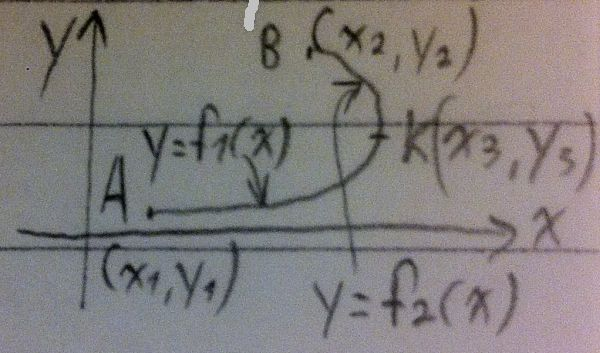
\includegraphics[scale=0.4]{intDividedPath}
	\caption{Function divided to multiple sections to be integrated}
	\label{fig:intDividedPath}
	\end{figure}
		
	\textbullet \quad Line integral relation with arc length: \linebreak 
	$\displaystyle I = \int_{AB} f ds = \int_{AB} (Pdx + Qdy) = \int_{c^{x_1}}^{x_2} f(x,y) \sqrt{1+ \left( \frac{dy}{dx} \right)^2} dx$ \linebreak 
	\textbullet \quad When $x$ and $y$ are expressed in parametric form, i.e. $x=f(t) \ , \ y=g(t)$, then: $\displaystyle I = \int_c f(x,y) ds = \int_{t_1}^{t_2} f(x,y) \sqrt{\left( \frac{dx}{dt} \right)^2 + \left( \frac{dy}{dt} \right)^2} dt $ \linebreak 
	\textbullet \quad If $Pdx + Qdy$ is an exact differential where $P,Q$ and their first derivatives are finite and continuous inside the simply connected region $R$, then  
	\begin{enumerate}
	\item $\displaystyle I = \int_c \left( Pdx + Qdy \right)$ is independent of the path of integration where $c$ lies entirely within $R$ 
	\item $\displaystyle I = \oint_c \left( Pdx + Qdy \right) $ is zero when $c$ is a closed curve lying entirely within $R$. 
	\end{enumerate} 
	Same reasoning applies for functions of more than two variables. \linebreak 
	
	\textbullet \quad \uline{Integration under the Integral Sign} is the use of the identity: \linebreak 
	$\displaystyle \int_a^b \int_{a_0}^a f(x,a) \ da \ dx = \int_{a_o}^a \int_a^b f(x,a) \ dx \ da $ to compute an integral of the form $\displaystyle  \int_{a_0}^a f(x,a) \ da $. It is also referred to as the Leibniz integral rule. \linebreak 
	
	\textbullet \quad \uline{Green's Theorem}: Let $P$ and $Q$ be two functions of $x$ and $y$ that are, along with their first partial derivatives, finite and continuous inside and on the boundary $c$ of a region $R$ in the $x-y$ plane. Then, by definition of G.T.: $\displaystyle \int_R \int \left( \frac{\partial P}{\partial y} - \frac{\partial Q}{\partial x} \right) dx dy = - \oint_c \left( P dx + Q dy \right) $ \linebreak 
	and for a simple closed curve: \linebreak 
	$\displaystyle \oint_c \left( xdy -ydx \right) = 2 \int_R \int dx dy = 2A$ , where $A$ is the area of the enclosed figure. \linebreak 
	\textbullet \quad $\displaystyle \int_R \int \ dx dy = $ Area of region $R$ \linebreak 
	\textbullet \quad Centre of gravity $\displaystyle (\overset{-}{x}, \overset{-}{y} ) \: M\overset{-}{x} = $ Sum of Moments about $x$-axis, $\displaystyle M\overset{-}{y} = $ Sum of moments about $y$-axis. \linebreak 
	Sum of moments about $x$-axis $\displaystyle  = \int_R \int xdm = \int_R \int x dy dx$ , \linebreak 
	Sum of moments about $y$-axis $\displaystyle = \int_R \int y dm$ \linebreak 
	\linebreak 
	
	\textbullet \quad \uline{Surface integrals}: $\displaystyle I = \int_R f(x,y) da = \int_R \int f(x,y) dy dx $ \linebreak 
	\textbullet \quad Surface in space: $\displaystyle I= \int_{S-} \phi (x,y,z) ds = \int_R \int \phi (x,y,z) \sec \gamma \ dx dy = \int_R \int \phi (x,y,z) \sqrt{1+ \left( \frac{\partial z}{\partial x} \right)^2 + \left( \frac{\partial z}{\partial y} \right)^2 } \ dx dy \ $, $\gamma < \frac{\pi}{2} $ , $z = f(x,y)$ \linebreak 
	$\phi(x,y,z)$  :  function of position on $S$ \linebreak 
	Area of the surface $\displaystyle s = \int_s ds = \int_R \int \sqrt{1 + \left( \frac{\partial z}{\partial x} \right)^2 + \left( \frac{\partial z}{\partial y}\right)^2 } \ dx dy$ \linebreak 
	$R$  :  projection of surface $s$ on $x-y$ plane. \linebreak 
	\textbullet \quad We project the surface $s$ onto the $x-y$ plane and then we use the variables $x,y,z$ such as: $\displaystyle ds = Adx dy$. $A$  :  scaling factor $\in \mathbb{R}$ \linebreak 
	\textbullet \quad The equation of $\phi (x,y,z) = $ constant  ,  represents a surface in space. [just like the equation $\displaystyle f(x,y) = \text{constant} (\text{e.g.} x+y=1)$ represents a line on a surface.] \linebreak 
	
	\textbullet \quad \uline{Volume integrals} \linebreak 
	We find: $1$) Volume of column, $2$) Volume of slice, $3$) Total volume \linebreak 
	\textbullet \quad $\displaystyle V = \int_{x_1}^{x_2} \int_{y_1}^{y_2} \int_{z_1}^{z_2} \ dz dy dx$ \linebreak 
	
	\textbullet \quad \uline{Change of variables in multiple integrals}: From Cartesian coordinates $(x,y)$ to Curvilinear coordinates $(u,v)$ \linebreak 
	a) Double Integrals, where $x=f(u,v) \ , y = g(u,v)$. Then: \linebreak 
	$\displaystyle I = \int_R \int f(x,y) dx dy = \int_R \int F\left( f(u,v) , g(u,v) \right) \big| \frac{\partial (x,y)}{\partial (u,v)} \big| \ du dv$ \linebreak 
	and $\displaystyle \big| \frac{\partial (x,y)}{\partial (u,v)} \big| \ du dv = dA$  :  the transformed element of area. \linebreak 
	b) Triple Integrals, where $x= f(u,v,w), y = g(u,v,w), z = h(u,v,w)$ , i.e. transformation in $3$ dimensions. \linebreak 
	$\displaystyle I= \int \int \int F(x,y,z) \ dx dy dz = \int \int \int G(u,v,w) \big| \frac{\partial (x,y,z)}{\partial (u,v,w)} \big| \ du dv dw$ \linebreak 
	and $\displaystyle  \big| \frac{\partial (x,y,z)}{\partial (u,v,w)} \big| \ du dv dw = dV$  :  the transformed element of volume \linebreak 
	
	\textbullet \quad $\displaystyle J(u,v,w) = \frac{\partial (x,y,z)}{\partial (u,v,w)} = 
	\begin{bmatrix}
	\frac{\partial x}{\partial u} & \frac{\partial y}{\partial u} & \frac{\partial z}{\partial u} \\ 
	\frac{\partial x}{\partial v} & \frac{\partial y}{\partial v} & \frac{\partial z}{\partial v} \\
	\frac{\partial x}{\partial w} & \frac{\partial y}{\partial w} & \frac{\partial z}{\partial w} \\
	\end{bmatrix}$ \linebreak 
	
	\subsubsection{Properties of Integrals}	
	
	\textbullet \quad An integral is the limit of a(n) (infinite) sum. \linebreak 
	\textbullet \quad $\displaystyle \int_a^b f(t) dt + \int_b^c f(t) dt = \int_a^c f(t) dt $ \linebreak 
	\textbullet \quad $\displaystyle \int_a^a f(t) dt = 0 $ \linebreak 
	\textbullet \quad $\displaystyle \int_a^b f(t) dt = -\int_b^a f(t) dt$ \linebreak 
	\textbullet \quad $\displaystyle \left| \int_a^b f(t) dt \leq \int_a^b |f(t)| dt \right| $ \linebreak 
	\textbullet \quad Distance interpretation of integral: Suppose $u(t)$ is the velocity at time $t$ of a particle moving along the $x$-axis. Then: $\displaystyle \int_a^b \left| u(t) \right| dt = S^+ + S^- = S $, where:  
	\begin{itemize}
		\renewcommand{\labelitemi}{$\rightarrow$}
	\item $S^+$  :  total distance traveled in the forward direction 
	\item $S^-$  :  total distance traveled in the backward direction 
	\item $S$  :  total distance traveled.
	whereas: $\displaystyle  \int_a^b u(t) dt = S^+ - S^- = D $ \linebreak 
	\item $S^+$  :  area bounded by $t$ axis, lines $t=a$ and $t=b$ and the part of the graph, where $f(t) \geq 0 $. 
	\item $S^-$  :  area bounded by $t$ axis, lines $t=a$ and $t=b$ and the part of the graph, where $f(t) \leq 0 $. 
	\item $D$  :  net displacement from the original position. 
	\end{itemize}
		
	\subsubsection{Integrals}
	
	\textbullet \quad $\displaystyle f(x) = 0 \rightarrow \int f(x) dx = C $ \linebreak 
	\textbullet \quad $\displaystyle f(x) = C \rightarrow \int f(x) dx = Cx = D $ \linebreak 
	\textbullet \quad $\displaystyle f(x) = x^a, \ a\in \mathbb{R} - \{-1\} \rightarrow \int f(x) = \frac{x^{a+1}}{a+1} + C $ \linebreak 
	\textbullet \quad $\displaystyle f(x) = \frac{1}{2\sqrt{x}}, x > 0 \rightarrow \int f(x) dx = \sqrt{x} + C$ \linebreak 
	\textbullet \quad $\displaystyle f(x) = \sin (x) \rightarrow \int f(x) dx = -\cos (x) + C $ \linebreak 
	\textbullet \quad $\displaystyle f(x) = \cos (x) \rightarrow \int f(x) dx = \sin (x) + C $ \linebreak 
	\textbullet \quad $\displaystyle f(x) = \frac{1}{\cos ^2(x)} \rightarrow \int f(x) dx = \tan (x) + C$ \linebreak 
	\textbullet \quad $\displaystyle f(x) = \frac{1}{\cos ^2(x)} \rightarrow \int f(x) dx = -\cot (x) + C$ \linebreak 
	\textbullet \quad $\displaystyle f(x) = e^x \rightarrow \int f(x) dx = e^x + C$ \linebreak 
	\textbullet \quad $\displaystyle f(x) = a^x\ , a \in \mathbb{R} - \{ 1 \} \rightarrow \int f(x) dx = \frac{a^x}{\ln (a)} + C $ \linebreak 
	\textbullet \quad $\displaystyle f(x) = \tan (x) \rightarrow \int f(x) dx = -\ln (|\cos (x)|) + C$ \linebreak 
	\textbullet \quad $\displaystyle f(x0 = \cot (x) \rightarrow \int f(x) dx = \ln (|\sin (x)|) + C $ \linebreak 
	\textbullet \quad $\displaystyle f(x) = \cos ^2(x) \rightarrow \int f(x) dx = \frac{1}{2} \left( x - \frac{\sin (2x)}{2} \right) + C $ \linebreak 
	\textbullet \quad $\displaystyle f(x) = \cos ^2(x) \rightarrow \int f(x) dx = \frac{1}{2} \left( x + \frac{\sin (2x)}{2} \right) + C $ \linebreak 
	\textbullet \quad $\displaystyle f(x) = \ln(x) \rightarrow \int f(x) dx = xln(x) -x + C \ $ (by substitution) \linebreak 
	\textbullet \quad $\displaystyle f(x) = \log_a (a) \rightarrow \int f(x) dx = x\log_a x - \frac{x}{\ln(a)} + C$ \linebreak 
	\textbullet \quad $\displaystyle f(x) =\frac{1}{x} \rightarrow \int f(x) dx = \begin{cases} \ln (x) + C\ , & x> 0 \\ 
																													  \ln (-x) + C\, & x < 0  \end{cases}
									 = \ln|x| + C$ \linebreak 
	\textbullet \quad $\displaystyle f(x) = \sin ^{-1} (x) \rightarrow \int f(x) dx = x \sin ^{-1} (x) + \sqrt{1-x^2} + C, \ |x| \leq 1 $ \linebreak 
	\textbullet \quad $\displaystyle f(x) = \cos ^{-1} (x) \rightarrow \int f(x) dx = x\cos ^{-1} (x) - \sqrt{1-x^2} + C, \ |x| \leq 1 $ \linebreak 
	\textbullet \quad $\displaystyle f(x) = \tan^{-1} (x) \rightarrow \int f(x) dx = x \tan^{-1} (x) -\frac{1}{2} \ln|1+x^2| + C $ \linebreak 
	\textbullet \quad $\displaystyle f(x) = \cot ^{-1} (x) \rightarrow \int f(x) dx = x \cot ^{-1} (x) + \frac{1}{2} \ln|1+x^2| + C $ \linebreak 
	\textbullet \quad $\displaystyle f(x) = \sinh (x) \rightarrow \int f(x) dx = \cosh (x) + C $ \linebreak 
	\textbullet \quad $\displaystyle f(x) = \cosh (x) \rightarrow \int f(x) dx = \sinh (x) + C $ \linebreak 
	\textbullet \quad $\displaystyle f(x) = \tanh (x) \rightarrow \int f(x) dx = \ln|\cosh (x)| + C$ \linebreak 
	\textbullet \quad $\displaystyle f(x) = \coth(x) \rightarrow \int f(x) dx = \ln|\sinh (x) | + C $ \linebreak 
	\textbullet \quad $\displaystyle f(x) = \sinh ^{-1} (x) \rightarrow \int f(x) dx = x \sinh ^{-1} (x) - \sqrt{x^2 + 1} + C $ \linebreak 
	\textbullet \quad $\displaystyle f(x) = \cosh ^{-1} (x) \rightarrow \int f(x) dx = x \cosh ^{-1} (x) - \sqrt{x^2 - 1} + C \ , \ x > 1$ \linebreak 
	\textbullet \quad $\displaystyle f(x) = \tanh ^{-1} (x) \rightarrow \int f(x) dx = x \tanh ^{-1} (x) + \frac{\ln(1-x^2)}{x} + C\ , \ |x| < 1 $ \linebreak 
	\textbullet \quad $\displaystyle f(x) = \coth ^{-1} (x) \rightarrow \int f(x) dx = c \coth ^{-1}(x) + \frac{\ln(x^2 -1)}{2} + C \ , \ |x| > 1 $ \linebreak 
	\textbullet \quad $\displaystyle f(x) = e^{-x^2} \rightarrow \int_{-\infty}^{\infty} f(x) dx = \sqrt{\pi}$ \linebreak 
	\textbullet \quad $\displaystyle f(x) = \tan ^2(x) \rightarrow \int f(x) dx = \tan x -x + C $ \linebreak 
	\textbullet \quad $\displaystyle f(x) = \frac{1}{x^2+a^2} \rightarrow \int f(x) dx = \frac{1}{a} \coth ^{-1} \left(\frac{x}{a}\right) $ \linebreak 
	\textbullet \quad $\displaystyle f(x) = \frac{1}{x^2-a^2} \rightarrow \int f(x) dx = -\frac{1}{a} \coth ^{-1} \left( \frac{x}{a} \right), \ x^2 > a^2 $ \linebreak 
	\textbullet \quad $\displaystyle f(x) = \sin (ax) \rightarrow \int f(x) dx = -\frac{1}{a} \cos (ax) $ \linebreak 
	\textbullet \quad $\displaystyle \int f'(x) e^{f(x)} dx = e^{f(x)} + C$ \linebreak 
	\textbullet \quad $\displaystyle \int f'(x) a^{f(x)} dx = \frac{a^{f(x)}}{\ln(a)} + C $ \linebreak 
	\textbullet \quad $\displaystyle \int f'(x) \ \left(f(x)\right)^a dx = \frac{\left[ f(x) \right]^{a+1}}{a+1} + C $ \linebreak 
	\textbullet \quad $\displaystyle f(t) = \delta (t) \rightarrow \int_{-\infty}^{\infty} f(t) dt_i = 1 \land \int_{-\infty}^t f(t_i) dt_i = u(t) $ \linebreak 
	\textbullet \quad $\displaystyle f(t) = u(t) \rightarrow \int_{-\infty}^t f(t_i) \ dt_i = r(t)\ , \ r(t) = \ \begin{cases} t\ , & t\geq 0 \\ 0\ , & t < 0 \end{cases} $ \linebreak 
	\textbullet \quad $\displaystyle f(x) = \sinh (ax) dx \rightarrow \int f(x) dx = \frac{1}{a} \cosh (ax) + C$ \linebreak 
	\textbullet \quad $\displaystyle f(x) = \sinh ^2 (ax) \rightarrow \int f(x) dx = \frac{1}{4a} \sinh (2ax) - \frac{x}{2} + C$ \linebreak 
	\textbullet \quad $\displaystyle f(x) = \cosh ^2(ax) \rightarrow \int f(x) dx = \frac{1}{4a} \sinh (2ax) + \frac{x}{2} + C$ \linebreak 
	\textbullet \quad $\displaystyle f(x) = \tanh ^2(ax) \rightarrow \int f(x) dx = x - \frac{\tanh (ax)}{a} + C$ \linebreak 
	\textbullet \quad $\displaystyle f(x) = \sec (x) \rightarrow \int f(x) dx = \ln \big( \frac{1+\sin (x)}{\cos (x)} \big) + C$ \linebreak 

	\textbullet \quad $\displaystyle f(Z) = \frac{1}{Z^2 -A^2} \rightarrow \int f(Z) dZ = \frac{1}{2A} \ln \left(\frac{Z-A}{Z+A} \right) + C$ \linebreak 
	\textbullet \quad $\displaystyle f(Z) = \frac{1}{A^2 -Z^2} \rightarrow \int f(Z) dZ = \frac{1}{2A} \ln \left(\frac{A+Z}{A-Z} \right) + C$ \linebreak 
	\textbullet \quad $\displaystyle f(Z) = \frac{1}{A^2 + Z^2} \rightarrow \frac{1}{A} \tan^{-1} \left( \frac{Z}{A} \right) + C$ \linebreak 
	\textbullet \quad $\displaystyle f(Z) = \frac{1}{\sqrt{A^2 -Z^2}} \rightarrow \int f(Z) dZ = \sin ^{-1} \left( \frac{Z}{A} \right) + C$ (the root keeps us from using partial fraction decomposition) \linebreak 
	\textbullet \quad $\displaystyle f(Z) = \frac{1}{\sqrt{A^2 +Z^2}} \rightarrow \int f(Z) dZ = \sinh ^{-1} \left( \frac{Z}{A} \right) + C$ \linebreak 
	\textbullet \quad $\displaystyle f(Z) = \frac{1}{\sqrt{Z^2 -A^2}} \rightarrow \int f(Z) dZ = \cosh ^{-1} \left( \frac{Z}{A} \right) + C$ \linebreak 
	\textbullet \quad $\displaystyle f(Z) = \sqrt{A^2-Z^2} \rightarrow \int f(Z) dZ = \frac{A^2}{2} \big[ \sin ^{-1} \left( \frac{Z}{A} \right) + \frac{Z\sqrt{A^2 -Z^2}}{A^2} \big] + C$ \linebreak 
	\textbullet \quad $\displaystyle f(Z) = \sqrt{Z^2+A^2} \rightarrow \int f(Z) dZ = \frac{A^2}{2} \big[ \sinh ^{-1} \left( \frac{Z}{A} \right) + \frac{Z\sqrt{A^2 +Z^2}}{A^2} \big] + C$ \linebreak 
	\textbullet \quad $\displaystyle f(Z) = \sqrt{Z^2-A^2} \rightarrow \int f(Z) dZ = \frac{A^2}{2} \big[ -\cosh ^{-1} \left( \frac{Z}{A} \right) + \frac{Z\sqrt{Z^2 -A^2}}{A^2} \big] + C$ \linebreak 
	\textbullet \quad $\displaystyle f(x) \int \frac{1}{a+b\sin ^2(x) + c\cos ^2(x)} dx\ , \ t=\tan (x)\ , \ \sin (x) =\frac{t}{\sqrt{1+t^2}} \ , \ dx= \frac{2dt}{1+t^2} \ , \ \cos (x) = \frac{1}{\sqrt{1+t^2}} $ \linebreak 
	\textbullet \quad $\displaystyle f(x) \int \frac{1}{a+b\sin (x) + c \cos (x)} dx\ , \ t=\tan (\frac{x}{2})\ , \ \sin (x) =\frac{2t}{1+t^2} \ , \ dx= \frac{2dt}{1+t^2} \ , \ \cos (x) = \frac{1-t^2}{1+t^2} $ \linebreak 
	\textbullet \quad $\displaystyle f(x) = \frac{1}{g(x)} \rightarrow \int f(x) dx = \ln(g(x)) \ $, if the highest power of $x$ is 1. Else: resort to partial fraction decomposition method. \linebreak 
	\textbullet \quad $\displaystyle f(x) = \cosec (x) \rightarrow \int f(x) dx = - \ln (|\cosec (x) + \cot (x) | ) + C$ \linebreak 
	\textbullet \quad $\displaystyle \pi = 2 e \ \int_0^{+\infty} \frac{\cos (x)}{x^2 + 1} dx $ \linebreak 
	\textbullet \quad $\displaystyle f(x) = \sec (x) \rightarrow \int f(x) dx = \ln (|\sec (x) + \tan (x) | ) + C$ \linebreak 
	\textbullet \quad $\displaystyle f(x) = e^{-x^2} \rightarrow \int_{0}^{\infty} f(x) dx = \frac{\sqrt{\pi}}{2}\ , \ \int_{-\infty}^{\infty} f(x) dx = \sqrt{\pi} $ \linebreak 
	\textbullet \quad $\displaystyle f(x) = e^{\frac{-x^2}{2}} \rightarrow \int_{-\infty}^{\infty} f(x) dx = \sqrt{2\pi} $ \linebreak 
	\textbullet \quad $\displaystyle f(x) = e^{-k^2x^2} \rightarrow \int_{0}^{\infty} f(x) dx = \frac{\sqrt{\pi}}{2k} \ , \ k>0$ \linebreak 
	
	Integrals of periodic functions (primarily to assist with Fourier series expansions) - applied for any interval of length $2\pi$ - \linebreak 
	\textbullet \quad $\displaystyle \int_{-\pi}^{\pi} dx = \left[ x \right]_{-\pi}^{\pi} = 2\pi $ \linebreak 
	\textbullet \quad $\displaystyle \int_{-\pi}^{\pi} \cos (nx) dx = 0 $ \linebreak 
	\textbullet \quad $\displaystyle \int_{-\pi}^{\pi} \sin (nx) dx = 0 $ \linebreak 
	\textbullet \quad $\displaystyle \int_{-\pi}^{\pi} \cos (mx) \cos (nx) dx = \pi \delta_{mn} $ \linebreak 
	\textbullet \quad $\displaystyle \int_{-\pi}^{\pi} \sin (mx) \sin (nx) dx = \pi \delta_{mn} $ \linebreak 
	\textbullet \quad $\displaystyle \int_{-\pi}^{\pi} \cos (mx) \sin (nx) dx = 0 $ \linebreak 
	
	\subsubsection{Reduction Formulae}

	$n \in \mathbb{N}^* $ \linebreak 
	\textbullet \quad $\displaystyle I_n = \int e^{nx} \sin (x) dx \rightarrow I_n = \frac{e^{nx}}{n^2+1} \ \left(n \sin (x) - \cos (x) \right)	 $ \linebreak 
	\textbullet \quad $\displaystyle I_n = \int \sin ^n(x) dx \rightarrow I_n = - \frac{1}{n} \sin ^{n-1} (x) \cdot \cos (x) + \frac{n-1}{n} I_{n-2} $ \linebreak 
	\textbullet \quad $\displaystyle I_n = \int \cos ^n(x) dx \rightarrow I_n = \frac{1}{n} \cos ^{n-1} (x) \cdot \sin (x) + \frac{n-1}{n} I_{n-1} $ \linebreak 
	\textbullet \quad $\displaystyle I_n = \int x^n e^x dx \rightarrow I_n = x^n e^x - n I_{n-1} $ \linebreak 
	\textbullet \quad $\displaystyle I_n = \int x^n \sin (x) dx \rightarrow I_n = -x^n \cos (x) + nx^{n-1} \sin (x) -n(n-1) \cdot I_{n-2} $ \linebreak 
	\textbullet \quad $\displaystyle I_n = \int x^n \cos (x) dx \rightarrow I_n = x^n \sin (x) + nx^{n-1} \cos (x) -n(n-1) I_{n-2} $ \linebreak 
	\textbullet \quad $\displaystyle I_n = \int \tan^n(x) dx \rightarrow I_n = \frac{\tan^{n-1}(x)}{n-1} - I_{n-2} (+C) $ \linebreak 
	\textbullet \quad \uline{Walli's Formula}: If $\displaystyle  I_n = \int_0^{\pi / 2} \sin ^n(x) dx\ $, or $\ I_n = \int_0^{\pi / 2} \cos ^n(x) dx $ then: $\displaystyle I_n = \frac{n-1}{n} I_{n-2} \ , \ I_0 = \frac{\pi}{2} \ , \ I_1 = 1 $ \linebreak 
	or $\displaystyle I_n = \frac{n-1}{n} \cdot \frac{n-3}{n-2} \cdot \frac{n-5}{n-4}  \cdot \cdots \begin{cases} \cdot 1 & (n\ \text{odd}) \\ 
																																						 \cdot \frac{\pi}{2} & (n \ \text{even} \end{cases} $ \linebreak 
	\textbullet \quad $\displaystyle I_n = \int \left(\ln(x) \right)^n dx \rightarrow I_n = x \left( \ln(x) \right)^n - nI_{n-1} $ \linebreak 
	\textbullet \quad $\displaystyle I_n = \int \cot ^n(x) dx\ , \ n>1 \rightarrow I_n = - \frac{\cot ^{n-1}(x)}{n-1} - I_{n-2}  = -\frac{\cot ^{n-1}(x)}{n-1} + \frac{\cot ^{n-3}(x)}{n-3} - \frac{\cot ^{n-5}(x)}{n-5} \pm \cdots \pm x + C$ \linebreak 
	\textbullet \quad $\displaystyle I_n = \int \left( x^2 + a^2 \right)^n dx \rightarrow I_n = \frac{1}{2n+1} \left[ x(x^2 + a^2)^n +2na^2 I_{n-1} \right] $ \linebreak 
	\textbullet \quad $\displaystyle I_n = \int \sec ^n(x) dx \rightarrow I_n = \frac{1}{n-1} \tan (x) \sec ^{n-2}(x) + \frac{n-2}{n-1} I_{n-1} \ , \ n\geq 2 $ \linebreak 
	\textbullet \quad $\displaystyle I_n = \int_0^{\pi} e^{-x} \sin ^n (x) dx \rightarrow I_n = \frac{n(n-1)}{n^2+ 1} \cdot I_{n-1} $ \linebreak 
	\textbullet \quad $\displaystyle I_n = \int_0^{\frac{\pi}{2}} x\cos ^n(x) dx \ , \ n>1 \rightarrow I_n = \frac{n(n-1)I_{n-2} - 1}{n^2} $ \linebreak 
	\textbullet \quad $\displaystyle I_n = \int_0^{\infty} x^n e^{-ax} dx \rightarrow I_n = \frac{n}{a} I_{n-1} \ \therefore I_n = \frac{n!}{a^{n+1}} $ \linebreak 
	\textbullet \quad $\displaystyle I_{m,n} = \int_0^{\frac{\pi}{2}} \sin ^m(x) \cdot \cos ^n(x) dx \rightarrow I_{m,n} = \frac{m-1}{m+n} \int_0^{\frac{\pi}{2}} \sin ^{m-2} (x) \cos ^n(x) \ dx $ or $ \ I_{m,n} = \frac{n-1}{m+n} I_{m-2, n} $ \linebreak 
	
	\uline{Improper integral}: The limit of a definite integral as an endpoint of the interval(s) of integration approaches either a specified real number, or $\infty$, or $-\infty$ or in some cases, as both endpoints approach limits. Symbolically: \linebreak 
	$\displaystyle \lim_{b\to \infty} \int_a^b f(x) dx \big[ = \int_a^{\infty} f(x) dx \big]$, or e.g.  \linebreak 
	$\displaystyle \lim_{c\to b^-} \int_a^c f(x) dx \ , \ \lim_{c\to a^+} \int_c^b f(x) dx$ \linebreak 
	$\displaystyle \int_{-\infty}^{\infty} f(x) dx = \int_{-\infty}^0 f(x) dx + \int_0^{\infty} f(x) dx$ \linebreak 
	
	
	\pagebreak
	
	
	\section{Differential Equations}

	\textbullet \quad Solutions to differential equations are functions, as opposed to algebraic equations where the solutions are numbers. \linebreak 
	\textbullet \quad An $n$th order differential equation is derived from a function having $n$ arbitrary constants. \linebreak 
	\textbullet \quad The general, or primitive, solution of the equation contains the arbitrary constant. \linebreak 
	\textbullet \quad The particular solution of the equation can be found if we are told the value of $y$ for a given value of $x$. Then we can find a value of $C$. \linebreak 

	\subsection{Ordinary Differential Equations (ODEs)}
	
	\textbullet \quad An \uline{ordinary differential equation (ODE)} is a differential equation containing one or more functions of one independent variable and its derivatives. The term ordinary is used in contrast with the term partial differential equation which may be with respect to more than one independent variable. \linebreak 
	
	\subsubsection{Analytical Solutions to ODEs}
	
	\uline{Solution of 1st order Differential Equations} \linebreak 
	\textbullet \quad a) By direct integration: $\displaystyle \frac{dy}{dx} = f(x) $, gives $y=\int f(x) dx$ \linebreak 
	\textbullet \quad b) By separating the variables: $\displaystyle F(y) \frac{dy}{dx} = f(x) $, gives $\int F(y) dy = \int f(x) dx $ \linebreak 
	\textbullet \quad c) Homogeneous equations: Substituting $y = v x$, gives $v + x \frac{dv}{dx} = F(v)$, which can be solved by separating the variables. \linebreak 
	Homogeneous equations are of the form: $\displaystyle a_n(x)y^{(n)} + a_{n-1}(x)y^{(n-1)} + \ldots + a_1(x)y' + a_0(x)y = 0$, where all the terms are proportional to either $y$, or a derivative of $x$. There's no $x$ \uline{alone}. \linebreak 
	\textbullet \quad d) Linear equations - Use of Integrating Factor (IF) \linebreak 
	They have the form: $\displaystyle \frac{dy}{dx} + Py = Q$, where $P \text{\&} Q$ are constants, or functions of $x$. \linebreak 
	Multiplying both sides by the IF = $\displaystyle e^{\int P(x) dx}$, gives $\displaystyle \frac{dy}{dx}\text{IF} + y \frac{d\text{IF}}{dx} = Q\cdot \text{IF} \rightarrow \frac{d}{dx} \{ y\text{IF} \} = Q \cdot \text{IF} \rightarrow y \text{IF} = \int Q \cdot \text{IF} dx $ \linebreak 
	\textbullet \quad e) Bernoulli's equation: $\displaystyle \frac{dy}{dx} + Py = Q y^n$ \linebreak 
	First, divide by $y^n$. Then put $z=y^{1-n}$. Afterwards it is reduced to type d. \linebreak 
	\textbullet \quad f) In various cases there may need to happen a specific transformation in order for the differential equation to fall to one of the previous categories. We transform a non-linear O.D.E. to a linear one this way. \linebreak 
	
	\uline{Second Order Differential Equations} \linebreak 
	\textbullet \quad Solution of equations of the form: $\displaystyle a\frac{d^2y}{dx^2} + b\frac{dy}{dx} + cy = f(x) $ \linebreak 
	Auxiliary equation: $am^2 +bm +c = 0 $ \linebreak 
	Types of solutions: \linebreak 
	a) Real and different roots: $m=m_1 \ \land m=m_2$ \linebreak 
	C.F.: $y=Ae^{m_1x} + Be^{m_2x} $ \linebreak 
	b) Real and equal roots: $m = m_1 (\text{twice})$ \linebreak 
	C.F.: $y = e^{m_1x} (A+Bx)$ \linebreak 
	c) Complex roots: $m=a\pm \beta x$ \linebreak 
	C.F.: $y = e^{ax} (A\cos \beta x + B\sin \beta x) $ \linebreak 
	
	\textbullet \quad Equations of the form: $\displaystyle \frac{d^2y}{dx^2} +n^2y = 0$ \linebreak 
	Auxiliary equation: $m^2=-n^2$ \linebreak 
	C.F.: $y=A\cos nx + B\sin nx$ \linebreak 
	\textbullet \quad Equations of the form: $\frac{d^y}{dx^2} -n^2y = 0$ \linebreak 
	Auxiliary equation: $m^2 =n^2$ \linebreak 
	C.F.: $\displaystyle y=A \cosh (nx) + B \sinh (nx) = e^{nx} \left( \frac{A+B}{2} \right) +e^{-nx} \left( \frac{A-B}{2} \right)$ \linebreak 
	\textbullet \quad General Solution = Complementary Function + Particular Integral [G.S. = C.F. + P.I.] \linebreak 
	\textbullet \quad To find C.F. solve: $\displaystyle a\frac{d^y}{dx^2} +b\frac{dy}{dx} +cy = 0$ \linebreak 
	\textbullet \quad Particular Integral exists only when $f(x) \neq 0$, i.e. in inhomogeneous differential equations. \linebreak 
	\textbullet \quad To find P.I. assume the general form of the R.H.S. It can be of the form: \linebreak 
	$f(x) = k \ldots$ \qquad Assume: $y_{PI} = C$ \linebreak 
	$f(x) = kx \ldots$ \qquad Assume: $y_{PI} =Cx + D$ \linebreak 
	$f(x) = kx^2$ \qquad Assume: $y_{PI} = Cx^2 +Dx +E$ \linebreak 
	$\displaystyle f(x) = k\sin (x)\ , \ \text{or} k\cos (x)$ Assume: $\displaystyle y_{PI} = C \cos (x) + D\sin (x) $ \linebreak 
	$\displaystyle f(x) = k \sinh (x) \ , \text{or} k \cosh (x)$ Assume: $\displaystyle y_{PI} = C \cosh (x) + D\sinh (x)$ \linebreak 
	$f(x) = e^{kx} $ \qquad Assume: $y_{PI} = Ce^{kx} $ \linebreak 
	Combine forms where applicable. Afterwards differentiate $y_{PI}$ to get $\frac{dy}{dx}$ and $\frac{d^2y}{dx^2}$, substitute to the L.H.S. to find the constants $C, D, \ldots$ by equating coefficients of the L.H.S. to those in the R.H.S. \linebreak 
	\textbullet \quad Note: If the general form of the R.H.S. is already included in the C.F., multiply $y_{PI}$ by $x$ as many times as necessary and proceed as before. \linebreak 
	\textbullet \quad Particular solution: Finding the values of the arbitrary constants $A$ and $B$, when given the necessary boundary / initial conditions. \linebreak 
	
	\textbullet \quad $\displaystyle f(t) = a \cos \sqrt{\frac{k}{l}} t + b \sqrt{\frac{l}{k}} \sin \sqrt{\frac{k}{l}} t$  :  Behaviour of a system that executes simple harmonic, oscillatory motion with natural frequency $\omega = \sqrt{\frac{k}{l}}$. Such a system is called a harmonic oscillator. \linebreak 
	\textbullet \quad $Af''(t) + Bf'(t) + Cf(t) = 0 $  :  Differential equation describing the position of the harmonic oscillator \linebreak 
	\textbullet \quad $f'(t)$  :  damping term, $B$  :  damping parameter \linebreak 
	With $0$ on the R.H.S. only transient terms exist in $f(t)$ (i.e. damping terms that decay over time t). With terms on the R.H.S. steady-state terms emerge. \linebreak 
	The R.H.S. is the forcing function. If this function's frequency is the same as the $\omega$ of the H.O. then the system will resonate, which means that it will oscillate with increasing amplitude. \linebreak 
	\uline{Leibnitz $n$ th derivative theorem}: $\displaystyle \left[ u=f(x) \land v = g(x) \right] \rightarrow (uv)^{(n)} = u^{(n)}v + ^nC_1 u^{(n-1)} v^{(1)} + ^nC_2u^{(n-2)} v^{(2)} + \ldots + ^nC_{n-1}u^{(1)}v^{(n-1)} + uv^{(n)} \ , \ u^{(0)} \equiv u$ \linebreak 
	\textbullet \quad \uline{Leibnitz - MacLaurin (power series) method} for solving O.D.E.'s of the form: $\displaystyle \frac{d^y}{dx^2} + P(x) \frac{dy}{dx} + Q(x) y = 0$ \linebreak 
	Steps: \linebreak 
	a) Differentiate given equation $n$ times \linebreak 
	b) Rearrange the result to obtain the recurrence relation between the derivatives, at $x=0$ (initial condition). \linebreak 
	c) Determine the values of the derivatives at $x=0$, usually in terms of $y(0)$ and $y'(0)$. \linebreak 
	d) Substitute the findings in the MacLaurin expansion for $y=f(x)$. \linebreak 
	e) Simplify the result where possible and apply boundary conditions if provided. \linebreak 
	\textbullet \quad \uline{Cauchy-Euler equi-dimensional equations} have the structure: \linebreak 
	$\displaystyle a_nx^n y^{(n)} (x) + a_{n-1}x^{n-1} y^{(n-1)} (x) + \ldots + a_1 xy'(x) + a_0 y(x) = g(x) $, where the coefficient of the $n$th derivative contains $x^n$ term. \linebreak 
	General solution = $y_H(x) + y_p(x)$, normally. We assume $y_n(x) = kx^n$, find its derivatives and substitute to find as many $n$'s as the degree of the equation. The form of the particular solution depends upon the form of the R.H.S. of the equation. \linebreak 
	
	\textbullet \quad \uline{Sturm - Liouville systems}: $\displaystyle (p(x) \cdot y')' + ( q(x) + \lambda r(x)) y = 0$, for $a \leq x \leq b$ and $r(x) > 0$, with boundary conditions $\displaystyle a_1 \cdot y(a) + a_2 \cdot y'(a) = 0$ and $\displaystyle \beta_1 \cdot y(b) + \beta_2 \cdot y'(b) = 0$ \linebreak 
	Solutions $y_n$ to a Sturm - Liouville system are called eigenvectors, each corresponding to an eigenvalue $\lambda_n$ for $n = 0,1,2, \ldots$ \linebreak 
	
	\subsubsection{Systems of Differential Equations}
	
	\textbullet \quad \uline{Solving systems of 1st order D.E.s}, of the form: \linebreak 
	$\displaystyle \textbf{F}'(x) = \textbf{A} \cdot \textbf{F}(x)\ $, where $\displaystyle \textbf{F}(x) = \begin{pmatrix}
		f_1(x) \\ f_2(x) \\ \vdots \\ f_n(x)
	\end{pmatrix}$ \& $\displaystyle \textbf{F}'(x) = \begin{pmatrix} f_1'(x) \\ f_2'(x) \\ \vdots \\ f_n'(x) \end{pmatrix} $  
	\begin{enumerate}
	\item Find the eigenvalues and eigenvectors of $\textbf{A}$ and construct the modal matrix $\textbf{M}$ and spectral matrix $\textbf{S}$, where eigenvalues are $\lambda_1, \lambda_2, \ldots, \lambda_n$ and eigenvectors $\textbf{C}_1, \textbf{C}_2, \ldots, \textbf{C}_n$. 
	\item Write the solution of the equation as $\displaystyle \textbf{F}(x) = \sum \limits_{r=1}^n a_r e^{\lambda_r x} \textbf{C}_r$ and use the boundary conditions to find the values of $a_r$, for $r=1,2,\ldots, n$.
	\end{enumerate} 
	
	\textbullet \quad \uline{Solving systems of 2nd order D.E.s}, of the form: $\displaystyle \textbf{F}''(x) = \textbf{A} \textbf{F}(x)$  
	\begin{enumerate}
	\item Find the eigenvalues $\lambda_1, \lambda_2, \ldots, \lambda_n$ of $\textbf{A}$. 
	\item Assuming the eigenvalues are all distinct, find the associated eigenvectors $\displaystyle \textbf{C}_1, \textbf{C}_2, \ldots, \textbf{C}_n$. 
	\item Write the solution of the equation as $\displaystyle \textbf{F}(x) = \sum \limits_{r=1}^n \big( a_re^{\sqrt{\lambda_r} \cdot x} + b_r e^{-\sqrt{\lambda_r}x} \big) \textbf{C}_r $ \linebreak 
	and use the boundary conditions to determine the values of the constants $a_r$ and $b_r\ $, $r=1,2,\ldots, n$. 
	\end{enumerate} 
	
	\subsection{Partial Differential Equations (PDEs)} 
	
	\textbullet \quad A \uline{partial differential equation (PDE)} is a differential equation that contains unknown multivariable functions and their partial derivatives. (ODEs are a special case which deal with functions of a single variable and their derivatives.) PDEs are used to formulate problems involving functions of several variables, and are either solved by hand, or used to create a relevant computer model. \linebreak 
	\textbullet \quad Solution to $u=f(x,y,w,t,\ldots)$ \linebreak 
	\textbullet \quad Linear equations: If $u=u_1, u=u_2, u=u_3, \ldots $ are solutions, then the following is also a solution: $\displaystyle u=u_1 + u_2 +u_3 + \ldots + u_r + \ldots = \sum \limits_{r=1}^{\infty} u_r$ \linebreak 
	\textbullet \quad \uline{Wave equation}: Simulates transverse vibrations of an elastic string: $\displaystyle \frac{\partial^2 u}{\partial x^2} = \frac{1}{c^2} \cdot \frac{\partial^2 u}{\partial t^2} \ , \ u = f(x,t)$ \linebreak 
	\textbullet \quad \uline{Heat Conduction equation}: Heat flows in uniform finite bar: $\displaystyle \frac{\partial^2 u}{\partial x} = \frac{1}{c^2} \cdot \frac{\partial u}{\partial t} \ , \ c^2 = \frac{k}{\sigma \rho} \ $ \linebreak 
	$k$  :  thermal conductivity of material, $\sigma$  :  specific heat of the material, $\rho$  :  mass per unit length of bar \linebreak 
	\textbullet \quad \uline{Laplace's equation}: Distribution of a field over a plane area: $\displaystyle \frac{\partial^2 u}{\partial x^2} + \frac{\partial^2 u}{\partial y^2} + \frac{\partial^2 u}{\partial z^2} + ... = 0 \ , \ u = f(x,y,z,...) (u$ is a scalar function) \linebreak 
	It is also written as $\displaystyle \nabla^2 u = 0$ , or $\Delta u = 0$  
	
	\textbullet \quad Solution steps 
	\begin{enumerate}
	\item Assume a solution of the form: $u=X(x) \cdot T(t)$ 
	\item Transpose the equation by separation of the variables. Then $\displaystyle \frac{\partial u}{\partial x} = X'T \ , \ \frac{\partial^2 u}{\partial x^2} = X''T \ , \ \frac{\partial u}{\partial t} = T'X \ , \ \frac{\partial^2 u}{\partial t^2} = T''X$ 
	\item The two solutions are in the form: $\displaystyle X = (A \cos \rho x + B\sin \rho x) \cdot ( C\cos c \rho t + D \sin c \rho t) $ \linebreak 
	Then $\displaystyle u(x,t) = (A \cos \rho x + B \sin \rho x) \cdot ( C \cos c \rho t + D \sin c \rho t) $ 
	\item Putting $c \rho = \lambda$ we apply boundary conditions to determine $A$ and $B$. 
	\item List the eigenvalues and eigenfunctions for $n=1,2,3,\ldots$ and determine general solution as an infinite sum. 
	\item Apply the remaining initial, or boundary conditions and finally determine $C_r$ and $D_r$ by Fourier series techniques. 
	\end{enumerate}

	
	\pagebreak
	
	\section{Difference Equations}

	\textbullet \quad Any function $f$, where its input $n \in \mathbb{Z}$ is restricted to integer values has as output $f(n)$ in the form of a discrete sequence of numbers. Such a function is called a \uline{sequence}. \linebreak 
    \textbullet \quad A \uline{recurrence relation (\textgreek{Αναδρομική Σχέση})} is an equation that recursively defines a sequence, or a multidimensional array of values, once one or more initial terms are given: each further term of the sequence or array is defined as a function of the preceding terms. \linebreak 
    \textbullet \quad The term "difference equation" is frequently used to refer to any recurrence relation, but rigorously speaking it is a type of a recurrence relation. \linebreak 
	\textbullet \quad The prescription of a sequence, say $f(n) = 5n -2$, written as a recursive equation, with all the unknowns on one side: $f(n+1) - f(n) = 5$, is called a \uline{difference} equation. \linebreak 
	\textbullet \quad The order of a difference equation is taken from the maximum number of terms between any pair of terms. In order to solve a difference equation it is necessary to have as many initial terms as the order of the difference equation. \linebreak 
	\textbullet \quad The solution of a constant coefficient, linear recursive difference equation is of the form: $f(n) = f_h(n) + f_p(n)$ \linebreak 
	\textbullet \quad $f_h(n)$ is the solution to the homogeneous equation: $\displaystyle a_n f(n) + a_{n-1} f(n-1) + \ldots + a_{n-k} f(n-k) = 0 \ $ {\tiny $(I)$} ($k$ order) \linebreak 
	We assume that the above has a solution in the form of: $f(n) = cw^n \ , c, w\in \mathbb{R}^* \ , n \in \mathbb{Z}$ and we substitute $f(n)$ into the dif. eq. $(I)$. \linebreak 
	Factorizing we find the characteristic equation of the difference equation: \linebreak 
	$\displaystyle Kw^N \big\{ a_k w^k + a_{k-1} w^{k-1} + \ldots + a_2 w +a_1 \big\} = 0$, where $a_k$ are constants and find the roots $w_k, w_{k-1}, \ldots , w$. \linebreak 
	Then $f_h(n) = A \cdot w_k^n + B\cdot w_{k-1}^n + \ldots\ $. \linebreak 
	If we have 2 equal roots, we assume $Bn \cdot w^n$ is also a root of the difference equation $(I)$. \linebreak 
	\textbullet \quad $f_p(n)$ is the particular solution and to find it we assume a solution to the (now) inhomogeneous equation: $\displaystyle a_n f(n) + a_{n-1} f(n-1) + \ldots + a_{n-k} f(n-k) = g(n) \ $ {\tiny $(II)$}, according to: \linebreak 
	$\displaystyle \begin{bmatrix}
	g(n) & \text{Particular solution} \\ 
	\text{polynomial term} n^m & C_m n^m + C_{m-1} n^{m-1} + \ldots + C_1 n + C_0 \\ 
	\text{exponential} a^n & Ca^n \\ 
	a^n \cos (bn) \ , \ a^n \sin (bn) & a^n \left( C_1 \cos (bn) + C_2 \sin (bn) \right) 
	\end{bmatrix} $
	
	We substitute the particular solution into $(II)$ and equate coefficients between the L.H.S. and R.H.S. \linebreak 
	\textbullet \quad The general solution is $f(n) = f_h(n) + f_p(n)$ \linebreak 
	\textbullet \quad Finally, given the initial conditions, we find the constants $A, B, C, \ldots $ of the $f_h(n)$. \linebreak 
	

	\pagebreak
	
	
	\section{Complex Numbers}
	
	\textbullet \quad A complex number is a number that can be expressed in the form $a + bi$, where $a$ and $b$ are real numbers and $i$ is the imaginary unit, satisfying the equation $i^2 = -1$. In this expression, $a$ is the real part and $a$ is the imaginary part of the complex number. If $z=a+bi$, then $ \Re (z) = a \quad \Im (z) = b$. \linebreak 
	
	\textbullet \quad $\displaystyle j = \sqrt{-1}\ , j^2 = -1 \ , \ j^3 = -j \ , \ j^4 = 1$ \linebreak 
	\textbullet \quad $\displaystyle z=a+jb \ , \Re(z)=a \ \land \ \Im(z) = b$ \linebreak 
	\textbullet \quad $\displaystyle \overset{-}{z} = a -jb: $ Conjugate \linebreak 
	\textbullet \quad $\displaystyle z = r\left(\cos \theta + j \sin \theta \right) $  :  Polar form (\figref{argandDiagram}) \linebreak 
	$\displaystyle a = r \cos \theta\ , \ b = r\sin \theta \ , \ \theta = \angle z = \tan^{-1} \left(\frac{b}{a}\right) \ , \ |z| = r$ \linebreak 
	
	\begin{figure}[H]
	\centering
	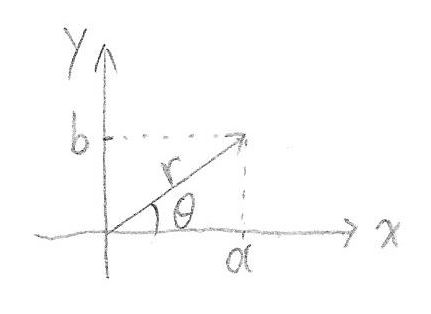
\includegraphics[scale=2]{argandDiagram}
	\caption{Argand Diagram}
	\label{fig:argandDiagram}
	\end{figure}	
	
	\textbullet \quad A \uline{phasor} (portmanteau for phase vector) is a term primarily used in circuit analysis, used to represent the amplitude and phase angle of a complex number (usually a voltage, or current). \linebreak 
	\textbullet \quad To find the correct angle $\theta$, we should beware that there are two angles between $0^{\circ}$ and $360^{\circ}$, the tangent of which has the value $b/a$. Always draw a sketch of the complex number to ensure we have the right quadrant. \linebreak 
	\textbullet \quad Those complex numbers that evaluate to $1$ when raised to some power $p$ are called the \uline{complex roots of unity}, ie. $\displaystyle z^p = 1 \Leftrightarrow (a + i\cdot b)^p = 1 $ \linebreak 
	For each $N$, there are exactly $N$ complex numbers $z$ such that $z^N = 1$. \linebreak 
	The numbers $\displaystyle \cos \Big( \frac{2\pi k}{N} \Big) + i \sin \Big( \frac{2\pi k}{N} \Big) $ for $k= 0, 1, \ldots , N-1$ can be easily shown to have this property. \linebreak 
	\textbullet \quad $\displaystyle z = \left| z \right| \efbox[rightline=false,topline=false]{z} \ (\angle z > 0), 
	\ \text{\textgreek{ή}} \ z= \left| z \right| \efbox[rightline=false,bottomline=false]{z} \ (\angle z < 0) $ \linebreak 
	\textbullet \quad $\displaystyle r=\sqrt{a^2 +b^2} $ \linebreak 
	\textbullet \quad $\displaystyle \tan (\theta) = \frac{b}{a} $ \linebreak 
	\textbullet \quad $\displaystyle |z|^2 = z \cdot \overset{-}{z} = r^2 $ \linebreak 
	\textbullet \quad $\displaystyle |z| = |\overset{-}{z} = |-z|$ \linebreak 
	\textbullet \quad $\displaystyle |z^{\nu} | = |z|^{\nu}$ \linebreak 
	\textbullet \quad $\displaystyle e^{\pm j\theta} = \cos \theta \pm j \sin \theta $  :  Oyler's identity \linebreak 
	\textbullet \quad $\displaystyle z=re^{j\theta} $  :  Exponential form. Here $\theta$ be in radians \linebreak 
	\textbullet \quad $\displaystyle \ln z = \ln r \pm j\theta $  :  Logarithm of complex number \linebreak 
	\textbullet \quad $\displaystyle z^n = \left[ r(\cos \theta + j \sin \theta \right]^n = r^n \left( \cos (n\theta) + j\sin (n\theta) \right) $ De'Moivre's Therorem, we can use it to find the roots of complex numbers \linebreak 
	\textbullet \quad $\displaystyle z + \frac{1}{z} = 2 \cos \theta $ \linebreak 
	\textbullet \quad $\displaystyle z^n + \frac{1}{z^n} = 2\cos (n\theta) $ \linebreak 
	\textbullet \quad $\displaystyle z -\frac{1}{z} = j2 \sin \theta $ \linebreak 
	\textbullet \quad $\displaystyle z^n - \frac{1}{z^n} = j2 \sin (n\theta)$ \linebreak 
	\textbullet \quad $\displaystyle \text{\textgreek{Από}} e^{jx} = \cos (x) + j\sin (x): ) \cos (x) = \frac{e^{jx} + e^{-jx}}{2} \ , \ \sin (x) = \frac{e^{jx}-e^{-jx}}{2j} $ \linebreak 
	
	\uline{Hyperbolic Functions} \linebreak 
	\textbullet \quad $\sinh (x) = \frac{e^x -e^{-x}}{2} $ \linebreak 
	\textbullet \quad $\cosh (x) = \frac{e^x + e^{-x}}{2} $ \linebreak 
	\textbullet \quad $e^{\pm x} = \cosh (x) \pm \sinh (x)$ \linebreak 
	\textbullet \quad $\displaystyle \tanh (x) = \frac{e^x -e^{-x}}{e^x +e^{-x}}$ \linebreak 
	\textbullet \quad $|f(e^{j\omega})|^2 = f(e^{j\omega}) \cdot f(e^{-j\omega}) $  :  \textgreek{Ταυτότητα του μέτρου} \linebreak 
	\textbullet \quad $\sinh ^{-1} (x) = \ln[x+ \sqrt{x^2 +1} ] $ \linebreak 
	\textbullet \quad $\cosh ^{-1} (x) = \pm \ln[x + \sqrt{x^2 -1} ] $ \linebreak 
	\textbullet \quad $\tanh ^{-1} (x) = \frac{1}{2} \ln \left( \frac{1+x}{1-x} \right) $ \ , \ output $ \in [-1,1] $ \linebreak 
	\textbullet \quad $\sin ^{-1} (x) = -j \ln[\sqrt{1-x^2} +jx] \ , \ -1 \leq x \leq 1 $ \linebreak 
	\textbullet \quad $\cos ^{-1} (x) = -j \ln[j\sqrt{1-x^2} + x ] \ , \ -1 \leq x \leq 1 $ \linebreak 
	\textbullet \quad $\tan^{-1} (x) = \frac{1}{2} j \ln \left( \frac{1-jx}{1+jx} \right) \ , \ \forall x \in \mathbb{R} $ \linebreak 
	\textbullet \quad $\coth(x) = \frac{1}{\tanh (x)}$ \linebreak 
	\textbullet \quad $\sech (x) = \frac{1}{\cosh (x)} $ \linebreak 
	\textbullet \quad $\cosech (x) = \frac{1}{\sinh (x)} $ \linebreak 
	\textbullet \quad $\cosh ^2 (x) - \sinh ^2 (x) = 1 $ \linebreak 
	\textbullet \quad $\sech ^2 (x) = 1 -\tanh ^2(x)$ \linebreak 
	\textbullet \quad $\cosech ^2(x) = \coth ^2(x) -1$ \linebreak 
	\textbullet \quad $\sinh (2x) = 2 \sinh (x) \cosh (x) $ \linebreak 
	\textbullet \quad $\cosh (2x) = \cosh ^2(x) + \sinh ^2(x) = 1 +2 \sinh ^2(x) = 2 \cosh ^2(x) - 1$ \linebreak 		
	
	\subsection{Complex Trigonometric \& Hyperbolic Identities} 
	
	\textbullet \quad $\sin (jx) = j \sinh (x) $ \linebreak 
	\textbullet \quad $\sinh (jx) = j \sin (x) $ \linebreak 
	\textbullet \quad $\cos (jx) = \cosh (x) $ \linebreak 
	\textbullet \quad $\cosh (jx) = \cos (x) $ \linebreak 
	\textbullet \quad $\tan (jx) = j\tanh (x) $ \linebreak 
	\textbullet \quad $\tanh (jx) = j\tan (x) $ \linebreak 
	\textbullet \quad $\Re [ \sinh (z) ] = \sinh (a) \cos (b) $ \linebreak 
	\textbullet \quad $\Im [ \sin (z) ] = \cosh (a) \sin (b) $ \linebreak 
	\textbullet \quad $\Re [ \cosh (z) ] = \cosh (a) \cos (b) $ \linebreak 
	\textbullet \quad $\Im [ \cos (z) ] = \sinh (a) \sin (b) $ \linebreak 
	\textbullet \quad $|\cosh (z) |^2 = \sinh ^2(a) + \cos ^2 (b) $ \linebreak 
	\textbullet \quad $|\sinh (z)|^2 = \sinh ^2(a) + \cos ^2 (b) $ \linebreak 
	\textbullet \quad $|x-y| = R \rightarrow x-y = Re^{j\theta} \ , \ x,y \in \mathbb{C}$ \linebreak 
	\textbullet \quad $\sin (z) = \frac{e^{jz} -e^{-jz}}{2j} $ \linebreak 
	\textbullet \quad $\cos (z) = \frac{e^{jz} + e^{-jz}}{2}$ \linebreak 
	\textbullet \quad $\displaystyle \tan (z) = \frac{\sin (z)}{\cos (z)} = \frac{e^{jz} - e^{-jz}}{e^{jz} + e^{-jz}} $ \linebreak 
	\textbullet \quad $\displaystyle \cot (z) = \frac{e^{jz} + e^{-jz}}{e^{jz} -e^{-jz}} $ \linebreak 
	\textbullet \quad $\cos (-z) = \cos (z) $ \linebreak 
	\textbullet \quad $\sin (-z) = - \sin (z) $ \linebreak 
	\textbullet \quad $\cos ^2(z) + \cos ^2 (z) = 1 $ \linebreak 
	\textbullet \quad $\cosh (z) = 0 \leftrightarrow z_0 = \pm j \left(n + \frac{1}{2} \right)\pi \ , \ n = 1,2, \ldots $ \linebreak 
	\textbullet \quad $\sinh (z) = 0 \leftrightarrow z_0 = \pm jn\pi \ , \ n=1,2,\ldots$ \linebreak 
	\textbullet \quad $\cosh \left(\sinh ^{-1} (x)\right) = \sqrt{x^2+1}$ \linebreak 
	\textbullet \quad $\sinh \left(\cosh ^{-1}(x)\right) = \sqrt{x^2-1} $ \linebreak 
	
	\textbullet \quad $\arctan \left( \frac{a}{S} \right) + \arctan \left( \frac{S}{a} \right) = \frac{\pi}{2} $ \linebreak 

	\begin{figure}[H]
	\centering
	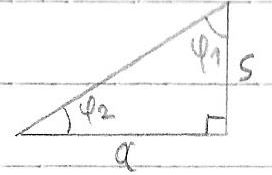
\includegraphics[scale=2.5]{complex_arctan}
	\caption{Visual representation of the identity}
	\label{fig:complex_arctan}
	\end{figure}

	\textbullet \quad $C \cdot f(t) \cdot \Re\{g(t) \} = C \Re\{ f(t) \cdot g(t) \} = \Re\{ C\cdot f(t) \cdot g(t) \} $ \linebreak 
	$\Re \ , \text{or} \Im \ , \mathbb{Z}\ , \text{etc} \ldots \ , \text{where} C \in \mathbb{C}$ \linebreak 

	\textbullet \quad \text{Hermitian function}: A complex function where its complex conjugate is equal to the original function with the variable changed in sign, i.e. $f^*(x) = f(-x) $ \linebreak 
	\textbullet \quad In linear algebra for an Hermitian matrix: $A^H = A^{-1} = \big(A^T\big)^* $ 
	Properties \linebreak 
	\textbullet \quad $\Re\{f(x) \} = \Re \{ f(-x) \} $ \linebreak 
	\textbullet \quad $\Im\{ f(-x) \} = - \Im \{ f(x) \} $, \linebreak 
	\textbullet \quad $|f(-x)| = |f(x) | $ \linebreak 
	\textbullet \quad $\angle f(-x) = - \angle f(x) $ \linebreak 
	\textbullet \quad Also: $f \bigstar g = f \bigstar g $ , if $f$ is Hermitian and \linebreak 
	\textbullet \quad $f \bigstar g = g \bigstar f $, if both $f$ and $g$ are Hermitian \linebreak 
	
	\textbullet \quad \uline{Transformation equation}: $z = x +jy \ \land w = u + jv $ \linebreak 
	Mappings from the $z$ plane, $z=f(x,y)$, onto the w-plane $w=f(z)\ z=x+jy\ , \ w=u+jv\ , \ u=g(x,y)\ , \ v=h(x,y) $ \linebreak 
	\textbullet \quad \uline{Linear Transformation}: $w=az + b$, where $a$ and $b$ are real or complex. A straight line in the z-plane maps onto a corresponding straight line the $w$-plane. \linebreak 
	\textbullet \quad Types of Linear transformations: $w=az+b$ \linebreak 
	a) \uline{Translation}: given by $b$ \linebreak 
	b) \uline{Magnification}: given by $|a|$ \linebreak 
	c) \uline{Rotation}: given by $ \text{arg} a$ \linebreak 
	\textbullet \quad \uline{Non-linear transformations} \linebreak 
	(a) $w=z^2$  :  A straight line through the origin maps onto a corresponding straight line through the origin in the w-plane. A straight line not passing through the origin maps onto a parabola. \linebreak 
	(b) $w=\frac{1}{z}$ (inversion): A straight line, or a circle maps onto a straight line, or a circle in the w-plane. A straight line may be regarded as a circle of infinite radius. ($z=1/w$  :  to find the equation) \linebreak 
	(c) $\displaystyle w=\frac{az+b}{cz+d} $ (bilinear transformation) - with $a,b,c,d$ real, or complex. \linebreak 
	\textbullet \quad Mapping of a region depends on the direction of development. \linebreak 
	Right (Left) hand regions map onto right (left) hand regions. \linebreak 
	
	\subsection{Complex Analysis}

	\textbullet \quad Complex analysis studies the properties of functions of complex numbers. \linebreak 
	
	\textbullet \quad \uline{Derivative of a function of a single real variable}: $y=f(x)$ \linebreak 
	$\delta y = f(x + \delta x) - f(x) $ \linebreak 
	$\displaystyle \frac{dy}{dx} = \lim_{\delta x \to } \left\{ \frac{f(x+\delta x) -f(x)}{\delta x} \right\} = \frac{(y+\delta y) -y}{\delta x} $ \linebreak 
		
	\begin{figure}[H] 
	\centering
	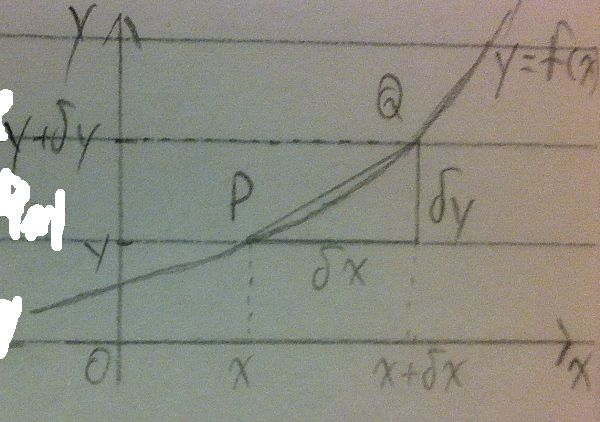
\includegraphics[scale=0.4]{complexAnalysisRealDerivative}
	\caption{Derivative of a function}
	\label{fig:complexAnalysisRealDerivative}
	\end{figure}
	
	\textbullet \quad \uline{Derivative of a function of a complex variable}: $w=f(z)$ \linebreak 
	$\displaystyle \left[ \frac{dw}{dz} \right]_{z_0} = \lim_{\delta z \to 0} \left\{ \frac{f(z_0 + \delta z) - f(z_0)}{\delta z} \right\} = \frac{(w+\delta w) - w}{\delta z} = \lim_{Q\to P} \frac{P'Q'}{PQ}$ \linebreak 
	If this limiting value exists, the function is said to be differentiable at $P$. \linebreak 
	\textbullet \quad $dz = dx + j dy \ , \ dw = du + j dv$ \linebreak 
	\textbullet \quad A function $w=f(z)$ is said to be \uline{regular}, or holomorphic, or \uline{analytic}, at a point $z=z_0$, if is defined and single valued and has a derivative at every point at and around $z_0$. Points in a region where $f(z)$ ceases to be regular (eg. its derivative does not exist) are called \uline{singular points}, or \uline{singularities}. A function of a complex variable that is analytic over the entire finite complex plane is called an \uline{entire function}. Examples of entire functions are polynomials, $e^z$, $\sin (z)$ and $\cos (z)$. \linebreak 	
	In other words, a \uline{holomorphic function} is a complex-valued function, of one or more complex variables that is complex differentiable in a neighborhood of every point in its domain. \linebreak 
	\textbullet \quad The real and imaginary parts of an analytic function are both harmonic and form a conjugate pair of functions. \linebreak 
	
	\textbullet \quad A \uline{meromorphic} function on an open subset D of the complex plane is a function that is holomorphic on all of D except for a set of isolated points, which are poles of the function. Every meromorphic function on D can be expressed as the ratio between two holomorphic functions (with the denominator not constant $0$) defined on $D$  :  any pole must coincide with a zero of the denominator. \linebreak 
	
	\textbullet \quad \uline{Cauchy - Riemann Equations}: A necessary condition for $w=f(z) = u+jv$ to be regular at $z=z_0$ is that $u=g(x,y)$ and $v=h(x,y)$ and their partial derivatives are continuous and that in the neighborhood of $z=z_0$  :  \linebreak 
	$\displaystyle \frac{\partial u}{\partial x} = \frac{\partial v}{\partial y} $ and $\frac{\partial v}{\partial x} = - \frac{\partial u}{\partial y}$ \linebreak 
	
	\textbullet \quad \uline{Complex Integration}: $\displaystyle \int wdz = \int f(z) dz = \int \left( udx -vdy \right) + j \int \left( vdx + udy \right) $ \linebreak 
	\textbullet \quad \uline{Contour Integration}: Evaluation of line integrals in the $z$-plane. 
	
	\textbullet \quad \uline{Cauchy's Theorem}: If $f(z)$ is regular at every point within and on a closed curve $c$, then \linebreak 
	$\displaystyle \oint_c f(z) dz = 0$ \linebreak 
	
	\textbullet \quad \uline{Deformation of Contours} \linebreak 

	(\textbf{a}) Singularity at $A$ (Multiple singularities may occur. \linebreak 
	(\textbf{b}) Restored to a closed curve. \linebreak 
	(\textbf{c}) $\displaystyle \oint_c f(z) dz = \oint_{c_1} f(z) dz$ \linebreak 
	
	For $\displaystyle \oint_c f(z) dz$ , where $\displaystyle f(z) = \frac{1}{(z-a)^n} \ , \ n = 1,2,3,\ldots $ \linebreak 
	$ \displaystyle \oint_c f(z) dz = 
		\begin{cases}		
			0 & n \neq 1 \\ 
			0 & n = 1 \text{and} c \text{does not enclose} a \\ 
			j2\pi & n=1 \text{and} c \text{does enclose} a		
		\end{cases} $ 	
	In general we have to consider if the singularity is enclosed within the contour $c$ (if that's not explicitly stated, or visible). \linebreak 
	
	\textbullet \quad If $f'(z_0) = 0$, at $z=z_0$, then $z_0$ is a \uline{critical point}. \linebreak 
	\textbullet \quad \uline{Conformal transformation}: mapping in which angles are preserved in size and sense of rotation. \linebreak 
	Conditions:  
	\begin{enumerate}
	\item $w=f(z)$ must be a regular function of $z$. 
	\item $f'(z)$, ie. $\displaystyle \frac{dw}{dz} \neq 0$ at a point of intersection. 
	\end{enumerate}

	\textbullet \quad \uline{Schwarz - Christoffel transformation}: maps any polygon in the $z$-plane onto the entire upper half of the $w$-plane and the boundary of the polygon onto the real axis of the $w$-plane. $\displaystyle \frac{dz}{dw} = A \left( w-u_1 \right)^{\frac{a_1}{\pi} -1} \cdot \left( w-u_2 \right)^{\frac{a_2}{\pi} -1} \ldots \left( w-u_n \right)^{\frac{a_n}{\pi} -1} $ \linebreak 
	We find $z$ from $\displaystyle \frac{dz}{dw}$ and finally the transformation function $w-f(z)$.  
	\begin{enumerate}
	\item Any three points $u_1, u_2,\ldots , u_n$ can be selected on the $u$-axis. $a_1, a_2, \ldots , a_n$ are the corresponding angles formed at the points $u_1,u_2,\ldots, u_n$ respectively. 
	\item One such point can be chosen at infinity. 
	\item Infinite open polygons are regarded as limiting cases of closed polygons. 
	\end{enumerate}
	
	\textbullet \quad If $f(z)$ is a function in the complex variable $z$, analytic at $z=0$, then its McLaurin series can be found by \linebreak 
	$\displaystyle f(z) = f(0) + zf'(0) + \frac{z^2}{2!} f''(0) + \frac{z^3}{3!} f'''(0) + \ldots $ \linebreak 
	
	\textbullet \quad \uline{Radius and circle of convergence}: The radius of the circle within which a series expansion is valid is called the raius of convergence of the series and the circle is called the circle of convergence. The radius of convergence can be found using the ratio test for convergence. When an expression is expanded in a McLaurin series, the circle of convergence is always centered on the origin and the radius of convergence is determined by the location of the first singular point met as $|z|$ moves out from the origin. \linebreak 
	\textbullet \quad If $f(z)$ has a singular point at $z_0$ and for some natural number $n$ the $\displaystyle \lim_{z\to z_0} \left\{ \left( z-z_0\right)^n f(z) \right\} = L \neq 0 $, then the singularity is called a \uline{pole} of order $n$ (the pole's multiplicity). \linebreak 
	\textbullet \quad If $f(z)$ has a singular point at $z_0$, but $\displaystyle \lim_{z\to z_0} \left\{ f(z) \right\}$ exists then the singular point is called a \uline{removable singularity}. \linebreak 
	
	\textbullet \quad \uline{Complex Taylor Series}: Provided $f(z)$ is analytic inside and on a simple closed curve $c$, the Taylor series expansion of $f(z)$ about a point $z_0$ which is interior to $c$ is given as: \linebreak 
	$\displaystyle f(z) = f(z_0) + (z-z_0) f'(z_0) + \frac{(z-z_0)^2 f''(z_0)}{2!} + \ldots + \frac{(z-z_0)^n f(z_0)^{(n)}}{n!} + \ldots $ \linebreak 
	where, here the expansion is about the point $z_0$ which is the centre of the circle of convergence. The circle of convergence is given as $|z-z_0| = R$, where $R$ is the radius of convergence. McLaurin's series is a special case of Taylor's series where $z_0 = 0$. It is easiest to derive the series with the new origin centered at $z_0$. For this purpose we can apply the transformation $u=z-z_0$. \linebreak 
	\textbullet \quad A derivable function of a complex variable is equal to the sum of its Taylor series. \linebreak 
	\textbullet \quad \uline{Laurent's series}: The Laurent series expansion provides a series expansion valid within an annular region centered on the singular point. Let $f(z)$ be singular at $z=z_0$ and let $c_1$ and $c_2$ be two concentric circles centered on $z_0$. Then if $f(z)$ is analytic in the annular region, between $c_1$ and $c_2$ and $c$ is any concentric circle lying within the annular region between $c_1$ and $c_2$, we can expand $f(x)$ as a Laurent series in the form: \linebreak 
	$\displaystyle f(z) = \ldots + \frac{a_{-2}}{(z-z_0)^2} + \frac{a_{-1}}{(z-z_0)} + a_0 + a_1 (z-z_0) + a_2 (z-z_0)^2 + \ldots = \sum \limits_{n\to -\infty}^{\infty} a_n \left( z-z_0 \right)^n$ \linebreak 
	where $\displaystyle a_n = \frac{1}{2\pi j} \oint \frac{f(z)}{(z-z_0)^{n+1}} dz$  :  \uline{Cauchy integral formula} \linebreak 
	for $\displaystyle r<\left|z-z_0\right| < R$ \linebreak 
	
	\textbullet \quad The part of the Laurent series that contains negative powers of the variable is called the \uline{principal part} of the series and the remaining terms constitute what is called the \uline{analytic part} of the series. If in the principal part the highest power of $1/z$ is $n$, then the function possesses a pole of order $n$ and if the principal part contains an infinite number of terms, the function possesses an \uline{essential singularity}. An essential singularity is a singularity that is neither a pole, nor a removable singularity. \linebreak 
	\textbullet \quad Removable singularities, poles and essential singularities are the three types that constitude the \uline{isolated singularities}. \linebreak 
	
	\textbullet \quad \uline{Residues}: In the Laurent series: $\displaystyle f(z) = \ldots + \frac{a_{-2}}{(z-z_0)^2} + \frac{a_{-1}}{z-z_0} + a_0 + a_1 (z-z_0) + a_2 (z-z_0)^2 + \ldots $ \linebreak 
	the coefficient $a_{-1}$ is referred to as the residue of $f(z)$. In other words, the residue of a function $f(z)$ is the coefficient of its $\displaystyle \frac{1}{z-a}$ term ($n-1$), when the function is expanded into its series representation. \linebreak 
	\textbullet \quad \uline{Calculating residues}: $\displaystyle a_{-1} = \lim_{z\to z_0} \left[ \frac{1}{(n-1)!} \frac{d^{n-1}}{dz^{n-1}} \left[ (z-z_0)^n f(z) \right] \right]$ \linebreak 
	where $n$ is the order of the pole. \linebreak 
	
	\textbullet \quad \uline{Cauchy's Residue Theorem}: Provided $f(z)$ is analytic at all points inside and on the simple closed contour $c$, apart from the single isolated singularity at $z_0$ which is interior to $c$, then $\displaystyle \oint_c f(z) dz = 2\pi ja_{-1}$ \linebreak 
	The residue theorem extends to the case where the contour contains a finite number of singularities. If $f(z)$ is analytic inside an on the simple closed contour $c$ except at the finite number of points $z_0, z_1, z_2, \ldots$ each with a Laurent series expansion and each with corresponding residues $ a_{-1}, a_{-1}, a_{-1}, \ldots $ then $\displaystyle \oint_c f(z) dz = 2\pi j \left\{ a_{-1} + a_{-1} + a_{-1} + \ldots \right\} $ \linebreak 
	
	\textbullet \quad \uline{Evaluation of certain real integrals} \linebreak 
	The Residue theorem can be very usefully employed to evaluate integrals of real functions. \linebreak 
	\textbf{-} Integrals of the form $\displaystyle \int_0^{2\pi} F(\cos \theta, \sin \theta) d\theta $ \linebreak 
	use $\displaystyle z=e^{j\theta}$ and $\displaystyle \cos \theta = \frac{(e^{j\theta} + e^{-j\theta}}{2} = \frac{z+z^{-1}}{2}$ \linebreak  
	$\sin \theta = \frac{e^{j\theta}-e^{-j\theta}}{2j} = {z-z^{-1}}{2j}$ \linebreak 
	and $\displaystyle dz = je^{j\theta} d\theta = jz d \theta$ \linebreak 
	so that $\displaystyle d\theta = \frac{dz}{jz}$. Convert the integral into a contour around the unit circle centered on the origin and use the Residue theorem. \linebreak 
	
	\textbf{-} Integrals of the form: $\displaystyle \int_{-\infty}^{\infty} F(x) dx$ and $\displaystyle \int_{-\infty}^{\infty} F(x) \begin{cases} \sin x \\ \cos x \end{cases} dx $ \linebreak 
	Consider integrals of the form $\displaystyle \oint F(z) dz$ and $\oint F(z) e^{jz} dz$ respectively, where the contour $c$ is a semicircle with the diameter lying along the real axis. The principle is that the integral can be evaluated by the Residue theorem and then the contour can be expanded to cover the required extent of the real axis, the integration along the semicircle giving a zero contribution. \linebreak 	
	
	\textbullet \quad An \uline{analytic function} is a function that is locally given by a convergent power series. There exist both real analytic functions and complex analytic functions, categories that are similar in some ways, but different in others. Functions of each type are infinitely differentiable, but complex analytic functions exhibit properties that do not hold generally for real analytic functions. A function is analytic if and only if its Taylor series about $x_0$ converges to the function in some neighborhood for every $x_0$ in its domain. \linebreak 
		
	\subsection{Quaternions}
	
	Quaternions is a number system that extends the complex numbers. They are generally represented in the form: \linebreak 
	$\displaystyle a + bi + cj + dk$ \linebreak 
	where $a$, $b$, $c$, and $d$ are real numbers, and $i$, $j$, and $k$ are the fundamental quaternion units. \linebreak 
	\textbullet \quad The quaternions are defined by the following equation: 
	$$ i^2 = j^2 = k^2 = ijk = -1 $$ 
	

	\pagebreak
	
	
	\section{Numerical Analysis}
	
	\textbullet \quad Numerical analysis is the study of algorithms that use numerical approximation (as opposed to general symbolic manipulations) for the problems of mathematical analysis. The field of numerical analysis developped as a necessity, because already known things from pure maths were unable to be applied in various branches of problems. So approximations had to be devised. \linebreak 
	
	\uline{Newton-Raphson Iterative method}  
	\begin{itemize}
		\renewcommand{\labelitemi}{$\rightarrow$} 
	\item First we try to find an approximate root of our real function in question, its $x$ value. Call it $x_1$. 
	\item Then we try to find a better approximation of that root, by using: $\displaystyle x_{n+1} = x_n - \frac{f(x_n)}{f'(x_n)} $ 
	\item The algorithm may not always work, especially when $f'(x_0)$ is very small. 
	\item It is used to find numerical solutions
	\end{itemize}
	\textbullet \quad Special case for finding $\sqrt{a}$ , $a$  :  number: $\displaystyle x_{i+1} = 0.5 (x_i + a / x_i)\ , \ i\in \mathbb{N} $ \begin{small} ($x_0$ is found by bisection) \end{small} 
	
	\uline{Modified / Enchanced Newton-Raphson method} \linebreak 
	When $f'(x_0)$ is very small then the Newton-Raphson method won't work, since $x_1$ might diverge from the real root. In such a case we calculate instead: \linebreak 
	$x_1 = x_0 \pm h$, where $\displaystyle h= \sqrt{\frac{-2f(x_0)}{f''(x_0)}}$. We choose $+h$ when $f(x_0)$ and $f''(x_0)$ have opposite signs and $-h$ when they are of equal sign. \linebreak 
	Afterwards we continue normally with $\displaystyle x_{n+1} = x_n - \frac{f(x_n)}{f'(x_n)}$ \linebreak 
	
	\uline{Interpolation}: A method of constructing new data points within the range of a discrete set of data points. \linebreak 
	\textbullet \quad Linear, Graphical (or approximate) \linebreak 
	From $2$ arbitrary points $p_1(x_1, y_1)$, $p_2(x_2, y_2)$ in a figure we want to find out the value $y$ somewhere in between $x_1$ and $x_2$, say @ $x$. We assume a linear dependence between $y_1$ and $y_2$. Then: \linebreak 
	$\displaystyle y = y_1 + (x-x_1) \frac{y_2 - y_1}{x_2 - x_1} $ \linebreak 
	\textbullet \quad Gregory-Newton formula using forward finite differences \linebreak 
	$\displaystyle f_p = f_0 + p \Delta f_0 + \frac{p (p-1)}{2!} \Delta^2 f_0 + \frac{p(p-1)(p-2)}{3!} \Delta^3 f_0 + \ldots $ \linebreak 
	\textbullet \quad Gregory-Newton formula using backward finite differences \linebreak 
	$\displaystyle f_p = f_0 + p \Delta f_{-1} + \frac{p(p+1)}{2!} \Delta^2 f_{-2} + \frac{p(p+1)(p+2)}{3!} \Delta^3 f_{-3} + \ldots$ \linebreak 
	Gauss interpolation using central finite differences \linebreak 
	\textbullet \quad Gauss forward formula \linebreak 
	$\displaystyle f_p = f_0 + p \delta f_{o+\frac{1}{2}} + \frac{p(p-1)}{2!} \delta^2 f_0 + \frac{(p+1)p(p-1)}{3!} \delta^3 f_{o+\frac{1}{2}} + \frac{(p+1)p(p-1)(p-2)}{4!} \delta^4 f_0$ \linebreak 
	\textbullet \quad Gauss backward formula \linebreak 
	$\displaystyle f_p = f_0 + p \delta f_{o-\frac{1}{2}} + \frac{p(p+1)}{2!} \delta^2 f_0 + \frac{(p+1)p(p-1)}{3!} \delta^3 f_{o-\frac{1}{2}} + \frac{(p+2)(p+1)p(p-1)}{4!} \delta^4 f_0 + \ldots $ \linebreak 
	in all cases: $\displaystyle h= x_1 -x_0\ , \ x_1 > x_0$  :  points that their $f(x_1), f(x_0)$ values are given and are closest to $x_p$. Also $\displaystyle x_0 < x_p < x_1 \ p = \frac{x_p - x_0}{h} $ \linebreak 
	\textbullet \quad Lagrangian Interpolation \linebreak 
	The interpolation polynomial of degree $n$ passes through $n+1$ points. To find the value $x$, not given in the data points $(x_j, f(x_j))$ we follow the formula: $\displaystyle p(x) = \sum_{j=0}^n l_j(x) f(x_j)$, where: $\displaystyle l_j(x) = \prod\limits_{0\leq i \leq n-1 \ i \neq j} \frac{x-x_i}{x_j-x_i}$ \linebreak 
	Lagrangian interpolation can also be used when the domain points are not equally spaced, sontrary to previous methods. \linebreak 	
	
	\uline{Frobenius} method for solving differential equations of the form: $\displaystyle y'' +P(x)\cdot y' + Q(x) \cdot y = 0$, under the conditions: \linebreak 
	(a) If functions $P(x) \land Q(x)$ are such that are both finite when $x$ is put equal to zero, $x=0$ is called an ordinary point of the equation. \linebreak 
	(b) If $\displaystyle x\cdot P(x)$ and $x^2 \cdot Q(x)$ remain finite at $x=0$, then $x=0$ is called a regular singular point of the d.eq. \linebreak 
	- If $P$ and $Q$ do not satisfy either of the conditions stated in (a), or (b), then $x=0$ is called an irregular singular point of the d.eq. and the method can't be applied.  
	\begin{itemize}
	\renewcommand{\labelitemi}{$\rightarrow$}
	\item Solution: We assume a series solution of the form: $\displaystyle y=x^c(a_0 +a_1x+a_2x^2+\ldots+a_rx^r+\ldots)\ , \ a_0 \neq 0$.
	\end{itemize}
	\begin{enumerate}
	\item Differentiate to find $y'$ and $y''$. They will be: \linebreak 
	$\displaystyle y'= a_0 c x^{c-1} +a_1 (c+1)x^c +a_2 (c+2) x^{c+1} + \ldots + a_r(c+r) x^{c+r-1} + \ldots$  \linebreak 
	$\displaystyle y'' = a_0c(c-1)x^{c-2} + a_1(c+1) cx^{c-1} +a_2(c+2)(c+1)x^c + \ldots + a_r(c+r)(c+r-1) x^{c+r-2} +\ldots$ 
	\item Substitute in the equation. 
	\item Equate coefficients of corresponding powers of $x$ on each side of the equation - usually written with zero on the R.H.S. and find the recurrence relation whose termin values all of the of the expansions
	\item Coefficient of the lowest power of $x$ gives the indicial equation from which the values of $c$ are obtained, $c=c_1$ and $c=c_2$. 
	\begin{itemize}
	\item \uline{Case 1}: $c_1$ and $c_2$ differ by a quantity not an integer. \linebreak 
	Substitute $c=c_1$ and $c=c_2$ in the series for $y$. 
	\item \uline{Case 2}: $c_1$ and $c_2$ differ by an integer and make a coefficient indeterminate when $c=c_1$. Substitute $c=c_1$ to obtain the complete solution. 
	\item \uline{Case 3}: $c_1$ and $c_2$ $(c_1 < c_2)$ differ by an integer and make a coefficient infinite when $c=c_1$. Replace $a_0$ by $k(c-c_1)$. Two independent solutions are then obtained by putting $c=c_1$ in the new series for $y$ and for $\displaystyle \frac{\partial y}{\partial c}$. In general if $c_1-c_2 = n$ where $n$ is a non zero integer, the solution is of the form: \linebreak 
	$\displaystyle y=(1+k \ln(x)) x^{c_1} \{a_0 +a_1x+a_2x^2+\ldots\} + x^{c_2}\{b_0 +b_1x+b_2x^2+\ldots\} $
	\item \uline{Case 4}: $c_1$ and $c_2$ are equal. Substitute $c=c_1$ in the series for $y$ and for $\displaystyle \frac{\partial y}{\partial c}$. Make the substitution after differentiating. In general if $c_1=c_2=c$, the solution is of the form: $\displaystyle y=(1+k \ln(x)) x^c \{a_0 +a_1x +a_2 x^2+\ldots \} + x^c \{b_1x +b_2 x^2 +\ldots \} $
	\end{itemize}
	\item For each value of $c$, consider values of $r=1,2,3, \ldots$ as needed and from the recurrence relation find the constants $a_1, a_2, a_3, a_4, \ldots$ in terms of $a_0$ or $a_1$. 
	\item Final solution is the sum of the series solutions found for the different values of $c$.
	\end{enumerate} 
	
	\subsubsection{Numerical Solutions to ODEs}
	
	\uline{Numerical Solutions to ODEs of order 1} \linebreak 
	$[$the subindex number is the $\#$ of iteration. With $0$ we denote the initial conditions$]$ \linebreak 
	\textbullet \quad Suppose we have the equation: $y' = f(x,y)$, with $y=y_0$ at $x=x_0$, for $x_0: h = x_n$  
	\begin{enumerate}
	\item Euler's Method \linebreak 
	$\displaystyle y_1=y_0 + h \cdot y_0'$ ($h$ is the step value, i.e. $x_{n+1} = x_n + h$) 
	\item Euler-Cauchy method \linebreak 
	$x_1 = x_0 + h$ \linebreak 
	$\displaystyle \overset{=}{y_1} = y_0 + h \cdot y_0'$  :  Auxilliary value of $y$ \linebreak 
	$\displaystyle y_1 = y_0 + 1/2 \cdot h \left[ y_0' + f(x_1, \overset{=}{y_1} \right] $ \linebreak 
	$\displaystyle y_1' = f(x_1,y_1)$ 
	\item Runge - Kutta method \linebreak 
	$\displaystyle x_1 = x_0 + h$ \linebreak 
	$\displaystyle k_1 = h \cdot f(x_0, y_0) = h \cdot y_0'$ \linebreak 
	$\displaystyle k_2 = h \cdot f (x_0 + 1/2 \cdot h, y_0 + 1/2 \cdot k_1)$ \linebreak 
	$\displaystyle k_3 = h \cdot f(x_0 + 1/2 \cdot h, y_0 + 1/2 \cdot k_2)$ \linebreak 
	$\displaystyle k_4 = h \cdot f(x_0 + h, y_0 + k_3)$ \linebreak 
	$\displaystyle \Delta y_0 = \frac{1}{6} ( k_1 + 2k_2 + 2k_3 + k_4)$ \linebreak 
	$\displaystyle y_1 = y_0 + \Delta y_0$ \linebreak 
	$\displaystyle y_1' = f(x_1, y_1)$ 
	\end{enumerate}  
	
	\uline{Numerical Solutions to ODEs of order 2} \linebreak 
	\textbullet \quad Suppose we have the equation: $y''= f(x,y,y')$, with $y=y_0$ and $y' = y_0'$ at $x=x_0$, for $x=x_0:h:x_n$.  
	\begin{enumerate}
	\item Euler's 2nd order method \linebreak 
	$\displaystyle y_1 = y_0 + h \cdot y_0' + \frac{h^2}{2!} \cdot y_0''$ \linebreak 
	$\displaystyle y_1' = y_0' + h\cdot y_0''$
	\item Ruge-Kutta method \linebreak 
	$\displaystyle x_1 = x_0 + h$ \linebreak 
	$\displaystyle k_1 = 1/2 \cdot h^2 \cdot f(x_0, y_0, y_0') = 1/2 \cdot h^2 \cdot y_0''$ \linebreak 
	$\displaystyle k_2 = 1/2 \cdot h^2 \cdot f(x_0 + 1/2 h, y_0 + 1/2 \cdot h \cdot y_0' + 1/4 k_1, y_0' + k_1 / h)$ \linebreak 
	$\displaystyle k_3 = 1/2 \cdot h^2 \cdot f(x_0 + 1/2 h, y_0 + 1/2 \cdot h \cdot y_0' + 1/4 k_1, y_0' + k_2 / h)$ \linebreak 
	$\displaystyle k_4 = 1/2 \cdot h^2 \cdot f(x_0 + h, y_0 + h\cdot y_0' + k_3, y_0' + 2k_3 / h)$ \linebreak 
	$\displaystyle P = 1/3 \cdot (k_1 + k_2 + k_3)$ \linebreak 
	$\displaystyle Q= 1/3 \cdot (k_1 + 2k_2 + 2k_3 + k_4)$ \linebreak 
	$\displaystyle y_1 = y_0 + h\cdot y_0' + P$ \linebreak 
	$\displaystyle y_1' = y_0' + Q/h$ \linebreak 
	$\displaystyle y_1'' = f(x_1, y_1, y_1')$ 
	\end{enumerate}  
	
	\textbullet \quad \uline{Predictor-Corrector numerical method for solving D.E.s} \linebreak 
	Employs a more accurate technique, where, instead of starting with just a single set of initial values, we use a collection of previously calculated values. \linebreak 
	Suppose we have the equation: $y' = f(x,y)$, with $y=y_0$ and $y' = y_0'$ at $x=x_0$, for $x:h:x_n$. Then \linebreak 
	Predictor: $\displaystyle \begin{cases} 
											\overset{-}{y_{i+1}} = y_i + 1/2 \cdot h (3f(x_i,y_i) -f(x_{i-1},y_{i-3})) & \ i =1,2,\ldots \\ 
											\overset{-}{y_1} = y_0 + h \cdot f(x_0,y_0) & i=0 
											\end{cases}$ \linebreak 
	Corrector: $\displaystyle y_{i+1} + 1/2 \cdot h \cdot (f(x_i,y_i) + f(x_{i+1}, \overset{-}{y}_{i+1})) \ \ i=0,1,2,3,\ldots $ \linebreak 
	
	\subsubsection{Numerical Solutions to PDEs} 
	
	\textbullet \quad Central difference formulas for partial direvatives. \linebreak 
	$[$ ($i$ column, $j$ row) $h,k$  :  distance between grid points on $x,y$ plane respectively.$]$ \linebreak 
	$\displaystyle \frac{\partial f(x,y)}{\partial x} \big|_{ij} = \frac{f_{i+1,j} -f_{i-1,j}}{2h} $ \linebreak 
	$\displaystyle \frac{\partial f(x,y)}{\partial y} \big|_{ij} = \frac{f_{i,j+1} -f_{i,j-1}}{2k} $ \linebreak 
	
	\textbullet \quad If $f(x,y)$ is signle valued, then to every domain point $(x,y)$ there corresponds a single range point $f(x,y)$. \linebreak 
	\textbullet \quad Grid alues: The value of $f(x,y)$ at the ijth grid point is denoted by: $f_{i,j} \equiv f(x_0 + ih, y_0 +jk)$ \linebreak 
	\textbullet \quad Computational molecules: The P.D.E.: $\displaystyle a\frac{\partial f(x,y)}{\partial x} + b \frac{\partial f(x,y)}{\partial y} = c$ , evaluated at the ijth grid point, is $\displaystyle a\frac{\partial f(x,y)}{\partial x} \big|_{ij} + b \frac{\partial f(x,y)}{\partial y} \big|_{ij} = c$ and is by the central difference formula: $\displaystyle \frac{a}{2h} (f_{i+1,j} -f_{i-1,j}) + \frac{b}{2k} ( f_{i,j+1} - f_{i,j-1} ) = c$ which is in turn represented by the composite computational molecule below (\figref{computationalMolecule}). \linebreak 
	
	\begin{figure}[H]
	\centering
	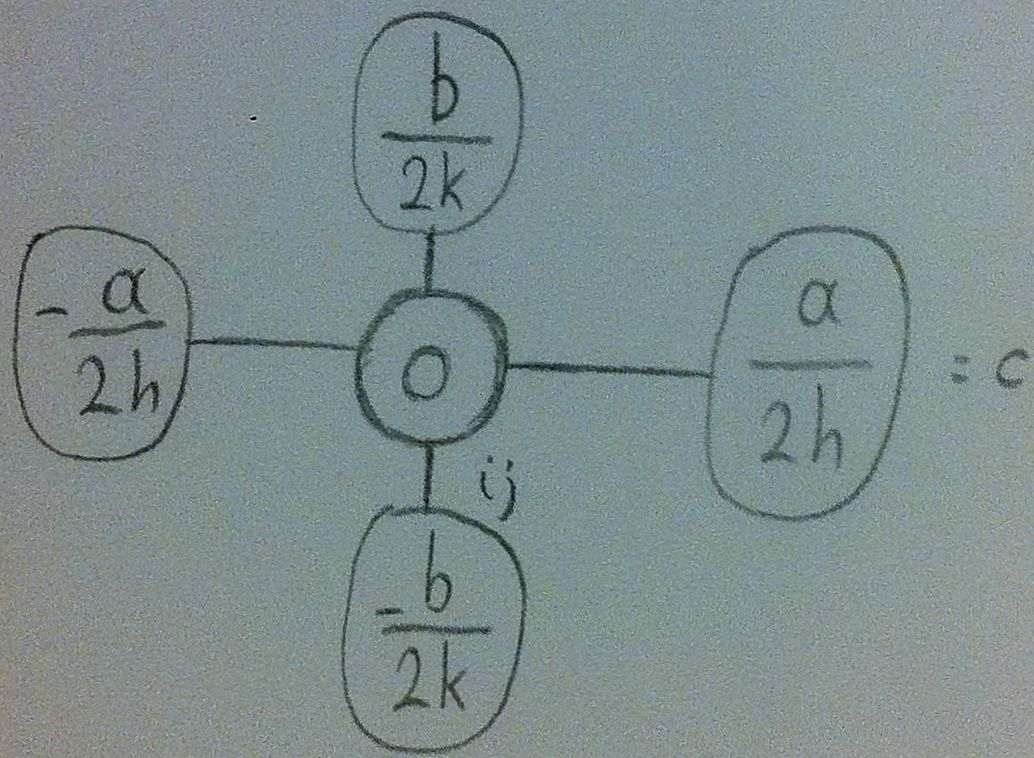
\includegraphics[scale=0.3]{computationalMolecule}
	\caption{Computational Molecule example}
	\label{fig:computationalMolecule}
	\end{figure} 
	
	\textbullet \quad The procedure to solve a 1st order P.D.E. is:  
	\begin{enumerate}
	\item Draw the function's domain with the grid overlaid. 
	\item On the drawing enter the values of $f(x,y)$ that can be obtained from the boundary conditions. 
	\item Label the grid points at which $f(x,y)$ is to be evaluated, with capital letters. 
	\item Construct the central difference equation that represents the numerical approximation to the P.D.E. 
	\item Construct the computational molecule for the P.D.E. 
	\item Lay the centre of the molecule on each of the lettered grid points in turn and derive a set of simultaneous linear equations - the unknowns being represented by the letters at the grid points. 
	\item Write the simultaneous equations in matrix form: $\textbf{A} \textbf{x} = \textbf{b}$ 
	\item Find $\textbf{A}^{-1}$ and computer the solution: $\textbf{x} = \textbf{A}^{-1} \textbf{b}$, finding the $f(x,y)$ values in the lettered grid points. 
	\end{enumerate} 

	\textbullet \quad If derivative boundary conditions exist, the grid is extended over the boundary of the function domain by adding additional points outside the domain appropriately, with values the value of the aforementioned derivative at the specified boundary point, i.e. @ $\displaystyle \frac{\partial f(x,y)}{\partial x} \big|_{x=x_0=C}$ ($x_0$ is b.point and $C=$value) \linebreak 
	
	\textbullet \quad \uline{Second Order P.D.E.s}: The most general form is: \linebreak 
	$$ a(x,y) \frac{\partial^2 f}{\partial x^2} + b(x,y) \frac{\partial^2 f}{\partial x \partial y} + c(x,y) \frac{\partial^f}{\partial y^2} + d(x,y) \frac{\partial f}{\partial x} + e(x,y) \frac{\partial f}{\partial y} + g(x,y) = 0 $$
	
	\textbullet \quad If $b^2 -4ac < 0$, then the P.D.E. is called an \uline{elliptic equation}. \linebreak 
	\textbullet \quad If $b^2 -4ac > 0$, then the P.D.E. is called a \uline{hyperbolic equation}. \linebreak 
	\textbullet \quad If $b^2 -4ac = 0$, then the P.D.E. is called a \uline{parabolic equation}. \linebreak 
	\textbullet \quad Central difference formulas for 2nd partial derivatives: \linebreak 
	$\displaystyle \frac{\partial^2 f(x,y)}{\partial x^2} \big|_{ij} \approx \frac{f_{i-1,j}-2f_{i,j}+f_{i+1,j}}{h^2} $ \linebreak 
	$\displaystyle \frac{\partial^2 f(x,y)}{\partial y^2} \big|_{ij} \approx \frac{f_{i,j-1} -2f_{i,j} + f_{i,j+1}}{k^2} $ \linebreak 
	
	\textbullet \quad \uline{Time Dependent Equations}: To use a central difference formula for the derivative with respect to $t$, would require knowledge of $f(x,t)$ for values $t<0$. Consequently, for a derivative with respect to $t$ we use the \uline{forward difference formula}: $\displaystyle \frac{\partial f(x,t)}{\partial t} \big|_{ij} \approx \frac{f_{i,j+1}-f_{i,j}}{k} $ \linebreak 
	So the P.D.E.: $\displaystyle \frac{\partial^2 f(x,t)}{\partial x^2} = \frac{\partial f(x,t)}{\partial t}$ , becomes $\displaystyle f_{i,j+1} = f_{i,j} + \frac{k}{h^2} \big( f_{i-1,j} -2f_{i,j} + f_{i+1,j} \big)$, where it can be shown that there will be no growth of rounding errors when evaluating this equation if: $\displaystyle \frac{k}{h^2} \leq \frac{1}{2}$ \linebreak 
	
	\textbullet \quad \uline{The Crank - Nicolson procedure} makes the assumption that the P.D.E. can be satisfied at points in time halfway between two grid points. That is: \linebreak 
	$\displaystyle \frac{\partial^2 f(x,t)}{\partial x^2} \big|_{i,j+1/2} = \frac{\partial f(x,t)}{\partial t} \big|_{i,j+1/2}$ This gives: \linebreak 
	$\displaystyle \frac{\partial f(x,t)}{\partial t} \big|_{i,j+1/2} = \frac{f_{i,j+1}-f_{i,j}}{2(k/2)} = \frac{f_{i,j+1}-f_{i,j}}{k}$ \linebreak 
	$\displaystyle \frac{\partial^2 f(x,t)}{\partial x^2} \big|_{i,j+1/2} = \frac{1}{2h^2} \big( f_{i-1,j} -2f_{i,j} + f_{i+1,j} + f_{i-1,j+1} -2f_{i,j+1} + f_{i+1,j+1} \big)$ \linebreak 
	Thus: $\displaystyle -f_{i,j+1} + \frac{k}{2h^2} \big( f_{i-1,j+1} -2f_{i,j+1} + f_{i+1,j+1} \big) = -f_{i,j} - \frac{k}{2h^2} \big( f_{i-1,j} -2f_{i,j} + f_{i+1,j} \big) $ \linebreak 
	, with no restriction on the value of $\displaystyle \frac{k}{2h^2}$ (usually we make it equal to $1$). \linebreak 

	
	\pagebreak
	
	
	\section{Vectors}
	
	\textbullet \quad $\vec{a} + \vec{b} = \vec{b} + \vec{a} $  :  \textgreek{Αντιμεταθετική ιδιότητα} \linebreak 
	\textbullet \quad $(\vec{a} + \vec{b} + \vec{c} = \vec{a} + (\vec{b} + \vec{c}) $  :  \textgreek{Προσεταιριστική ιδιότητα} \linebreak 
	\textbullet \quad $ \vec{AB} \leftleftarrows \vec{\Gamma \Delta} \rightarrow \vec{AB}, \vec{\Gamma \Delta} $  :  \textgreek{Ομόρροπα διανύσματα} \linebreak  
		\textbullet \quad $ \vec{AB} \leftrightarrows \vec{\Gamma \Delta} \rightarrow \vec{AB}, \vec{\Gamma \Delta} $  :  \textgreek{Αντίρροπα διανύσματα} \linebreak  
	\textbullet \quad $ \vec{AB} = -\vec{BA} $ \linebreak  
	\textbullet \quad $ \vec{AB} = \vec{OB} - \vec{OA} $ \textgreek{Ο: σημείο αναφοράς} \linebreak 
	$\vec{OA}, \vec{OB} $  :  \textgreek{διανυσματικές ακτίνες, ή διανύσματα θέσεως του Α και B} \linebreak 
	\textbullet \quad $ \left| |\vec{a}| - |\vec{b}| \right| \leq |\vec{a} + \vec{b}| \leq |\vec{a}| + |\vec{b}| $ \linebreak 
	\textbullet \quad $ \vec{a} + \vec{0} = \vec{a} $ \linebreak 
	\textbullet \quad $ \vec{a} + (-\vec{a}) = \vec{0} $ \linebreak 
	\textbullet \quad $ \lambda(\vec{a} + \vec{b}) = \lambda \vec{a} + \mu \vec{a} , \ \lambda \in \mathbb{R} $ \linebreak 
	\textbullet \quad $ (\lambda + \mu) \vec{a} = \lambda \vec{a} + \mu \vec{a} , \ \lambda, \mu, \in \mathbb{R} $ \linebreak 
	\textbullet \quad $ \lambda(\mu \vec{a}) = (\lambda \mu) \vec{a} , \ \lambda , \mu \in \mathbb{R} $ \linebreak 
	\textbullet \quad $ \forall \lambda, \mu \in \mathbb{R} \left[(\lambda \vec{a} = \lambda \vec{b} \land \lambda \neq 0 ) \rightarrow \vec{a} = \vec{b} \right] $ \linebreak 
	\textbullet \quad $ \forall \lambda, \mu \in \mathbb{R} \left[ (\lambda \vec{a} = \mu \vec{a} \land \vec{a} \neq 0) \rightarrow \lambda = \mu \right] $ \linebreak 
	\textbullet \quad $ \vec{a}, \vec{b} $ \textgreek{δύο διανύσματα} $, \vec{b} \neq 0 \rightarrow \left[ \vec{a} \parallel \vec{b} \leftrightarrow \exists \lambda \in \mathbb{R} (\vec{a} = \lambda \vec{b} ) \right] $ \linebreak 
	\textbullet \quad \textgreek{Διανυσματική ακτίνα μέσου τμήματος: } $ \vec{AB}: \ \vec{OM} = \frac{\vec{OA} + \vec{OB}}{2} $ \linebreak 
	\textbullet \quad \textgreek{Οι συντεταγμένες} $(x,y)$ \textgreek{του διανύσματος με άκρα τα σημεία αρχής} $A(x_1, y_1)$ \textgreek{και τέλους} $B(x_2,y_2)$ \textgreek{δίνονται από τις σχέσεις:} $x = x_2 -x_1\ \text{\&}\ y = y_2 + y_1 $ \linebreak 
	\textbullet \quad $ \vec{a} = (x,y) \rightarrow |\vec{a}| = \sqrt{x^2 +y^2}, |\vec{a}|: $ \textgreek{μέτρο διανύσματος} $ \vec{a}$ \linebreak 
	\textbullet \quad \textgreek{Η απόσταση των συμείων} $A(x_1, y_1)\ \text{\&}\ B(x_2, y_2) $ \textgreek{είναι ίση με} $(AB) = \sqrt{(x_2-x_1)^2 + (y_2 -y_1)^2} .$ \linebreak 
	\textbullet \quad \textgreek{Συντεταγμένες κέντρου βάρους τριγώνου} $A\overset{\triangle}{B}\Delta$, \textgreek{με} $A(x_1, y_1), B(x_2, y_2)\ \text{\&}\ \Gamma(x_3, y_3) $ \textgreek{είναι}: $\displaystyle x = \frac{x_1 + x_2 + x_3}{3}\ \text{\&}\ y = \frac{y_1 + y_2 + y_3}{3} . $ \linebreak  
	\textbullet \quad $\displaystyle  \vec{a} \parallel \vec{b} \leftrightarrow \det(\vec{a}, \vec{b}) = 0 , \ \det(\vec{a}, \vec{b}) = \begin{bmatrix} 
	x_1 & y_1 \\ 
	x_2 & y_2	
\end{bmatrix}, \vec{a} = (x_1, y_1), \vec{b} = (x_2, y_2) $ \linebreak 
	\textbullet \quad $ \lambda = \tan (\phi) = \frac{y}{x}: $ \textgreek{συντελεστής διεύθυνσης του διανύσματος} $ \vec{a} = (x,y), \phi: $ \textgreek{γωνία που σχηματίζει το διάνυσμα} $ \vec{a}$ \textgreek{με τον άξονα} $x'x$. \linebreak 
	\textbullet \quad $ \vec{a} \parallel \vec{b} \leftrightarrow \lambda_1 = \lambda_2 $  :  \textgreek{Συνθήκη παραλληλίας δύο διανυσμάτων} $ \vec{a}, \vec{b}$ \textgreek{με συντελεστές διεύθυνσης} $\lambda_1, \lambda_2$ \textgreek{αντίστοιχα}. \linebreak 
	\textbullet \quad $ \vec{a} = \lambda \vec{b} $. \textgreek{Αν} $ \vec{a}, \vec{b}$ \textgreek{ομόρροπα, τότε} $\lambda \geq 0$. \textgreek{Αν} $ \vec{a}, \vec{b}$ \textgreek{αντίρροπα τότε} $\lambda < 0$. \linebreak 
	\textbullet \quad $ \vec{a}, \vec{b} \neq 0 \rightarrow \left[ \vec{a} \cdot \vec{b} = | \vec{a} | \cdot |\vec{b}| \cos (\phi) \right] $ \textgreek{: Εσωτερικό γινόμενο διανυσμάτων} $ \vec{a} $ \textgreek{και} $ \vec{b}$. (\uline{Scalar Product}) \linebreak 
	$\overset{\wedge}{\phi} = $ \textgreek{γωνία που σχηματίζουν τα διανύσματα} $ \vec{a}, \vec{b}$ \textgreek{μεταξύ τους}. \linebreak 
	\textbullet \quad $ \vec{a} \perp \vec{b} \leftrightarrow \vec{a} \cdot \vec{b} = 0 $ \linebreak 
	\textbullet \quad $ \vec{a} \parallel \vec{b} \leftrightarrow \vec{a} \vec{b} = |\vec{a}||\vec{b}| $ \linebreak 
	\textbullet \quad $ \vec{a} \leftrightarrows \vec{b} \leftrightarrow \vec{a} \cdot \vec{b} = - |\vec{a}| |\vec{b}| $ \linebreak 
	\textbullet \quad $ \vec{a} \cdot \vec{a} = \vec{a}^2 = |\vec{a}|^2 $ \linebreak 
	\textbullet \quad $ \vec{a} = (x_1, y_1) \land \vec{b}(x_2, y_2) \rightarrow \vec{a} \cdot \vec{b} = x_1 x_2 + y_1 y_2 $  :  \textgreek{Αναλυτική έκφραση εσωτερικού γινομένου διανυσμάτων} $ \vec{a}, \vec{b}$. \linebreak 
	\textbullet \quad $(\lambda \vec{a})\cdot \vec{b} = \vec{a} \cdot (\lambda \vec{b}) = \lambda (\vec{a} \cdot \vec{b}) $ \linebreak 
	\textbullet \quad $ \vec{a} \cdot (\vec{b} + \vec{\gamma}) = \vec{a} \cdot \vec{b} + \vec{a} \cdot \vec{\gamma} $ \textgreek{Επιμεριστική ιδιότητα} \linebreak 
	\textbullet \quad $(\vec{a}, \vec{b} \nparallel y'y \land \vec{a} \perp \vec{b} ) \leftrightarrow \lambda_{\vec{a}} \cdot \lambda_{\vec{b}} = -1 $ \linebreak 
	\textbullet \quad $ \vec{\nu}, \vec{a} \neq \vec{0}, \text{\textgreek{με κοινή αρχή}} \rightarrow \vec{a} \cdot \vec{\nu} = \vec{a} \text{\textgreek{προβ}}_{\vec{a}} \vec{\nu} $ \qquad \textgreek{προβ}$_{\vec{a}} \vec{\nu} = \vec{OM}_1 $ \linebreak 

	\begin{figure}[H]
	\centering
	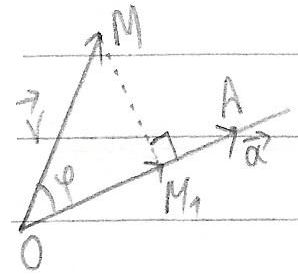
\includegraphics[scale=2]{vectorProjection}
	\caption{\textgreek{Προβολή διανύσματος}}
	\label{fig:vectorProjection}
	\end{figure}	
	
	\textbullet \quad \textgreek{Εμβαδό τριγώνου:} $\displaystyle  (A\overset{\triangle}{B}\Gamma) = \frac{1}{2} \left|\det\left(\vec{AB}, \vec{A\Gamma}\right) \right| $ \linebreak 
		\textbullet \quad $G$ centroid of $A\overset{triangle}{B}C \rightarrow \vec{GA} + \vec{GB} + \vec{GC} = \vec{0} $ \linebreak 
	
	\textbullet \quad \uline{Direction cosines}: The direction of a vector in 3 dimensions is determined by the angles which the vector makes with the three axes of reference. \\ Let $\displaystyle \overrightarrow{OP} = a\vec{i} + b\vec{j} + c\vec{k} $ be a vector. \\ 
	Then: $\displaystyle \frac{a}{r} = \cos (a) = l, \qquad \frac{b}{r} = \cos (b) = m, \qquad \frac{c}{r} = \cos (\gamma) = n $\\
			 $\displaystyle \qquad \qquad a = \angle(i, r), \qquad \qquad  b = \angle(j, r), \qquad \qquad \gamma = \angle(k, r) $ \\ 
	$ r= \sqrt{a^2 +b^2 +c^2}, \qquad a, b, c $  :  3 direction consines of vector $ r = \overrightarrow{OP}$.  \linebreak 
	
	\textbullet \quad  \uline{Vector/Cross Product} of two vectors: It acts in a direction perpendicular to both $ \vec{a}$ and $ \vec{b} $ \\ $\displaystyle  \therefore \left| \underbrace{\vec{a}}_{\text{(thumb)}} \times \underbrace{\vec{b}}_{\text{(index finger)}} \right| = \underbrace{|a|\cdot |b| \sin \theta}_{\text{(middle finger)  (can represent the area  of a parallelogram)}}$ \linebreak 
	$ \vec{i} \times \vec{j} = \vec{k} , \vec{j} \times \vec{k} = \vec{i}, \vec{k} \times \vec{i} = \vec{j} \quad (\vec{a}, \vec{b}\ \text{and} \left| \vec{a} \times \vec{b} \right| \text{form a right handed set}) $ \linebreak 
	$\displaystyle \vec{a} \times \vec{b} = \begin{bmatrix}
			i & j & k \\ 
			a_1 & a_2 & a_3 \\ 
			b_1 & b_2 & b_3	
	\end{bmatrix} = - \vec{b} \times \vec{a} $ \linebreak 
	Cross product represents the signed area of the parallelogram formed by the points, or vectors considered. \linebreak 
	
	\textbullet \quad  \uline{Angle between two vectors}. Let $ \vec{a}, \vec{b} $ vectors with direction cosines $[l, m, n]$ and $[l', m', n']$ respectively. Then $\cos \theta = \cos \angle(\vec{a}, \vec{b}) = ll' + mm' + nn' $ \linebreak 
	It can also be found by the scalar product of $ \vec{a}, \vec{b}$. 
	\textbullet \quad If $A(x_1, y_1), B(x_2, y_2), C(x_3, y_3)$ then the area of the formed triangle is: $\displaystyle  (A\overset{\triangle}{\text{\textgreek{Β}}}C) = \frac{1}{2} 
		\begin{bmatrix}
		1 & 1 & 1 \\
		x_1 & x_2 & x_3 \\ 
		y_1 & y_2 & y_3 
		\end{bmatrix} $ \linebreak 
		
	\textbullet \quad For perpendicular vectors: $ll' + mm' + nn' = 0$. \linebreak 
	\textbullet \quad For parallel vectors: $ll' + mm' + nn' = 1$. \linebreak 
	\textbullet \quad $\overrightarrow{A} \times (\vec{B} + \vec{C} = \vec{A} \times \vec{B} + \vec{A} \times \vec{C} $  :  Distributive property \linebreak 
	\textbullet \quad \uline{Scalar Triple product} of three vectors $\vec{A}(a_x, a_y, a_z), \vec{B}(b_x, b_y, b_z) \text{and} \vec{C}(c_x, c_y, c_z) $  :  \linebreak 
	$\displaystyle \vec{A} \cdot (\vec{B} \times \vec{C}) = \left|  
		\begin{bmatrix}
			a_x & a_y & a_z \\ 
			b_x & b_y & b_z \\ 
			c_x & c_y & c_z		
		\end{bmatrix} \right| $ \linebreak 
	\textbullet \quad $\vec{A} \cdot (\vec{B} \times \vec{C} = \vec{B} \cdot (\vec{C} \times \vec{A}) = \vec{C} \cdot ( \vec{A} \times \vec{B}) $  :  Unchanged by cyclic change of vectors. Sign reversed by non-cyclic change. \linebreak 
	\textbullet \quad $\left| \vec{A} \cdot (\vec{B} \times \vec{C}) \right| = |\vec{A}| \cdot |\vec{B}| \cdot |\vec{C}| \cdot |\sin ( \theta) \cdot \cos (\theta)| \equiv $	volume of the parallelepiped with 3 adjacent sides defined by $\vec{A}, \vec{B}, \vec{C}. $\\ 
	$\overset{\wedge}{\theta} = \angle(\vec{B}, \vec{C}), \overset{\wedge}{\phi} = \angle(\vec{A}, \vec{n}), |\vec{n}| = 1 $ \linebreak 
	\textbullet \quad $\vec{A} \cdot ( \vec{B} \times \vec{C}) = 0 \rightarrow \vec{A}, \vec{B}, \vec{C}$ vectors are coplanar \linebreak 
	\textbullet \quad \uline{Vector Triple Product} $\displaystyle  \vec{A} \times ( \vec{B} \times \vec{C}) = 
		\begin{bmatrix}
			\vec{i} & \vec{j} & \vec{k} \\
			a_x & a_y & a_z \\
			\begin{bmatrix}
				b_y & b_z \\ 
				c_y & c_z
			\end{bmatrix} &
			\begin{bmatrix}
				b_z & b_x \\ 
				c_z & c_x
			\end{bmatrix} &
			\begin{bmatrix}
				b_x & b_y \\ 
				c_x & c_y
			\end{bmatrix}
		\end{bmatrix} $ \linebreak 
	\textbullet \quad $ \vec{A} \times (\vec{B} \times \vec{C}) = (\vec{A} \cdot \vec{C}) \vec{B} - (\vec{A} \cdot \vec{B}) \vec{C}$ \linebreak 
	\textbullet \quad $(\vec{A} \times \vec{B}) \times \vec{C} = (\vec{C} \cdot \vec{A}) \vec{B} - (\vec{C} \cdot \vec{B}) \vec{A} $ \linebreak 	
	\textbullet \quad \uline{Vector Function}: $\vec{A}(u) = a_x(u)\cdot \vec{i} + a_y (u) \vec{j} + a_z (u) \cdot \vec{k} $ \linebreak 
	\textbullet \quad $\displaystyle  \frac{d\vec{A}}{du} = \frac{da_x}{du} \vec{i} + \frac{da_y}{du} \vec{j} + \frac{da_z}{du} \vec{k} $  :  Differentiation of vectors \linebreak 
	\textbullet \quad $\displaystyle T = \frac{dA/du}{\left| dA / du \right|} $  :  \uline{Unit (tangent) vector} parallel to the tangent to the curve at P \figref{unitTangentVector} \linebreak 
	
	\begin{figure}[H]
	\centering
	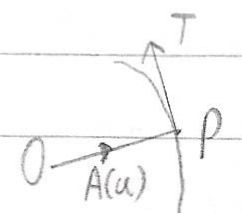
\includegraphics[scale=2]{unitTangentVector}
	\caption{Unit Tangent Vector}
	\label{fig:unitTangentVector}
	\end{figure}	
	
	\textbullet \quad $ \int_a^b \vec{A}(u) du = \vec{i} \int_a^b a_x du + \vec{j} \int_a^b a_y du + \vec{k} \int_a^b a_zdu $  :  Integration of vectors \linebreak 
	\textbullet \quad Most (if not all) standard calculus rules apply in vector functions. \linebreak 
	\textbullet \quad Transforming vector $\vec{A}$ into unit vector $\overset{\wedge}{a}$  :  \\ 
		$\displaystyle \overset{\wedge}{a} = \frac{a_x\vec{i} + a_y\vec{j}+a_z\vec{k}}{\left| \vec{A} \right|} = \frac{\vec{A}}{\left| \vec{A} \right|} $, with the direction of the original vector $ \vec{A} $ \linebreak 
		
	\textbullet \quad $ d\vec{r} = \vec{i} dx + \vec{j} dy + \vec{k} dz $ \linebreak 
	\textbullet \quad $ \vec{F} = F_x \vec{i} + F_y \vec{j} + F_z \vec{k} $ \linebreak 
	\textbullet \quad $ \vec{F} \cdot d\vec{r} = F_x dx + F_y dy + F_z dz $ \linebreak 
	\textbullet \quad $ \int_c \vec{F} \cdot d\vec{r} = \int_c F_x dx + \int_c F_y dy + \int_c F_z dz $ \linebreak 
	
	\subsection{Vector Analysis} 
	
	\textbullet \quad If every point $P(x,y,z)$ of a region $R$ of space has associated with it, a scalar quantity $\phi (x,y,z)$, then $\phi (x,y,z)$ is a \uline{scalar function} and a \uline{scalar field} is said to exist in the region $R$. \linebreak 
	\textbullet \quad Similarly, if every point $P(x,y,z)$ of a region $R$ has associated with it a vector quantity $\vec{F} (x,y,z)$, then $\vec{F} (x,y,z)$ is a \uline{vector function} and a \uline{vector field} is said to exist in the region $R$. \linebreak 
	\textbullet \quad \uline{Gradient of a scalar function $\phi (x,y,z)$} \linebreak 
	$\displaystyle \grad (\phi) = \vec{i} \frac{\partial \phi}{\partial x} + \vec{j} \frac{\partial \phi}{\partial y} + \vec{k} \frac{\partial \phi}{\partial z} = \left\{ \vec{i} \frac{\partial}{\partial x} + \vec{j} \frac{\partial}{\partial y} + \vec{k} \frac{\partial}{\partial z} \right\} \phi = \nabla \phi $ \linebreak 
	where $\nabla \equiv \left( \vec{i} \frac{\partial}{\partial x} + \vec{j} \frac{\partial}{\partial y} + \vec{k} \frac{\partial}{\partial z} \right) $  :  \uline{vector differential operator}, or del, or nabla operator \linebreak 
	and $\phi$ is continuously differentiable with respect to its variables $x,y,z$, throughout the region $R$. \linebreak 
	The gradient is a generalization of the usual concept of derivative to functions of several variables. If $f(x_1, ..., x_n)$ is a differentiable, real-valued function of several variables, its gradient is the vector whose components are the $n$ partial derivatives of $f$. It is thus a vector-valued function. \linebreak 
Similarly to the usual derivative, the gradient represents the slope of the tangent of the graph of the function. More precisely, the gradient points in the direction of the greatest rate of increase of the function, and its magnitude is the slope of the graph in that direction, ie. the direction of $\grad (\phi)$ gives the direction in which the maximum rate of change of $\phi$ occurs. \linebreak 
	\textbullet \quad Total differential of $\phi (x,y,z)$  :  \linebreak 
	$\displaystyle \grad (\phi) \cdot d\vec{r} = \left( \frac{\partial \phi}{\partial x} \vec{i} + \frac{\partial \phi}{\partial y} \vec{j} + \frac{\partial \phi}{\partial z} \vec{k} \right) \cdot \left( dx \cdot \vec{i} + dy \cdot \vec{j} + dz \cdot \vec{k} \right) = \frac{\partial \phi}{\partial x} dx + \frac{\partial \phi}{\partial y} dy + \frac{ \partial \phi}{\partial z} dz = d\phi$ \linebreak 
	Gradient Properties \linebreak 
	\textbullet \quad $\displaystyle \nabla (A + B) = \nabla A + \nabla B$  :  Grad of Sums \linebreak 
	\textbullet \quad $\displaystyle \nabla (A \cdot B) = A ( \nabla B) + B ( \nabla A)$  :  Grad of Products \linebreak 
	
	\textbullet \quad \uline{Directional Derivative} $\displaystyle \frac{d \phi}{d s} = \hat{a}\ \grad (\phi) = \hat{a} \nabla \phi $ \linebreak 
	where $\hat{a}$ is a unit vector in a stated direction. It gives the rate of change of $\phi$ with distance measured in the direction of $\hat{a}$. \linebreak 
	\textbullet \quad \uline{Unit normal vector} $N$ to surface: $\phi (x,y,z) = $ constant, $\displaystyle \vec{N} = \frac{\nabla \phi}{\left| \nabla \phi \right|} $ (at a point $P(x,y,z)$ ) \linebreak 
	
	\textbullet \quad \uline{Divergence (div) of a vector function $\vec{A}$ }: \linebreak 
	$\displaystyle \div (\vec{A}) = \nabla \cdot \vec{A} = \frac{\partial a_x}{\partial x} + \frac{\partial a_y}{\partial y} + \frac{\partial a_z}{\partial z} $ (notice the dot $\cdot$ in $\nabla$) \linebreak 
	Divergence is a vector operator that produces a signed scalar field giving the quantity of a vector field's source at each point. More technically, the divergence represents the volume density of the outward flux of a vector field from an infinitesimal volume around a given point. \linebreak 
	As an example, consider air as it is heated or cooled. The velocity of the air at each point defines a vector field. While air is heated in a region, it expands in all directions, and thus the velocity field points outward from that region. The divergence of the velocity field in that region would thus have a positive value. While the air is cooled and thus contracting, the divergence of the velocity has a negative value. \linebreak 
	\textbullet \quad If $\displaystyle \nabla \cdot \vec{A} = 0$ for all points, then $A$ is called a solenoidal vector. \linebreak 

	\textbullet \quad \uline{Curl of a vector function $\vec{A}$}: \linebreak 
	$\displaystyle \curl (A) = \nabla \times \vec{A} = \left( \vec{i} \frac{\partial}{\partial x} + \vec{j} \frac{\partial}{\partial y} + \vec{k} \frac{\partial}{\partial z} \right) \times \left( a_x \vec{i} + a_y \vec{j} + a_z \vec{k} \right) = 
	\begin{bmatrix}
		\vec{i} & \vec{j} & \vec{z} \\ 
		\frac{\partial}{\partial x} & \frac{\partial}{\partial y} & \frac{\partial }{\partial z} \\ 
		a_x & a_y & a_z 
	\end{bmatrix} $ \linebreak 
	The curl is a vector operator that describes the infinitesimal rotation of a 3-dimensional vector field. At every point in the field, the curl of that point is represented by a vector. The attributes of this vector (length and direction) characterize the rotation at that point. \linebreak 
	The direction of the curl is the axis of rotation, as determined by the right-hand rule, and the magnitude of the curl is the magnitude of rotation. \linebreak 
	\textbullet \quad If $\nabla \times \vec{A} = 0$ then the vector field $\vec{A}$ is said to be irrotational. \linebreak 
	
	\textbullet \quad \uline{Multiple Vector Operations} 
	\begin{itemize}
	\item $\displaystyle \curl \grad \phi = \nabla \times ( \nabla \phi ) = 0$ 
	\item $\displaystyle \div \curl \vec{A} = \nabla \cdot ( \nabla \times \vec{A} ) = 0$ 
	\item $\displaystyle \div \grad{\phi} = \nabla \cdot ( \nabla \phi) = \frac{\partial^2 \phi}{\partial x^2} + \frac{\partial ^2 \phi}{\partial y^2} + \frac{\partial ^2 \phi}{\partial z^2} = \partial ^2 \phi = \Delta $  :  Laplacian of $\phi$ 
	\item $\displaystyle \nabla \times ( \nabla \times \vec{A} ) = \nabla ( \nabla \cdot \vec{A} ) - \nabla^2 \vec{A} $ \linebreak
	\end{itemize} 
	 
	\textbullet \quad \uline{Surface Integrals} \linebreak 
	We note that a surface is defined by $\phi (x,y,z,) = $ constant \linebreak 
	\textbf{a}) \uline{Scalar field} $V(x,y,z)$  :  \linebreak 
	$\displaystyle \int_s V d\vec{s} = \int_s V \hat{n} ds $ , where $\hat{n} = \frac{ \nabla \phi}{\left| \nabla \phi \right|} $ \linebreak 
	\textbf{b}) \uline{Vector field} $\displaystyle \vec{F} = F_x \vec{i} + F_y \vec{j} + F_z \vec{k} $ \linebreak 	
	$\displaystyle \int_s \vec{F} \cdot d\vec{s} = \int_s \vec{F} \cdot \hat{n} ds$ , \linebreak 
	where $\hat{n} = \frac{\nabla \phi}{\left| \nabla \phi \right|} $ unit normal vector \linebreak 
	
	\textbullet \quad A vector field $\vec{F}$ is conservative if  
	\begin{enumerate}
	\item $\displaystyle \oint_c \vec{F} \cdot d\vec{r} = 0$ , for all closed curves \linebreak 
	\item $\displaystyle \curl \vec{F} = 0$ 
	\item $\vec{F} = \grad V$ 
	\end{enumerate}	
	The line integral of a conservative vector field is independent of the path of integration between the two end points. \linebreak 

	\textbullet \quad \uline{Harmonic function}: is a twice continuously differentiable function $f(x,y,z,...)$ that satisfies Laplace's equation. \linebreak 
	\textbullet \quad A \uline{smooth function} is a function that has derivatives of all orders everywhere in its domain. The \uline{smoothness} of a function is a property measured by the number of derivatives it has, which are continuous. \linebreak 		
	
	\textbullet \quad \uline{Divergence (Gauss's) Theorem} \linebreak 
	For a closed surface $S$ enclosing a region $V$ in a vector field $\vec{F}$  :  $\displaystyle \int_v \div \vec{F} dV = \int_S \vec{F} \cdot d \vec{S} $ \linebreak 
	for a closed surface the normal vectors at all points are drawn in an outward direction. \linebreak 
	
	\textbullet \quad \uline{Stoke's Theorem} \linebreak 
	Let an open surface $S$ bounded by a simple closed curve $c$. Then $\displaystyle \int_S \curl \vec{F} \cdot d \vec{S} = \oint_c \vec{F} \cdot d \vec{r} $ \linebreak 
	
	\textbullet \quad The unit normal $\hat{n}$ is drawn in a right - handed screw sense (common right hand rule). (convention) \linebreak 
	\textbullet \quad Sign convention for the surfaces is represented by the image below (\figref{surfaceConvention}) \linebreak 
	
	\begin{figure}[H]
	\centering
	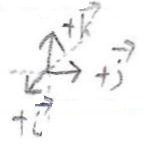
\includegraphics[scale=2.5]{surfaceConvention}
	\caption{Sign convention for surfaces}
	\label{fig:surfaceConvention}
	\end{figure}
	
	
	\pagebreak
	
	
	\section{Determinants}
	
	\textbullet \quad Considering the equations: \linebreak 
	$\displaystyle \begin{cases}
	a_1 x+b_1 y+c_1 z+d_1 =0 \\ 
	a_2 x+b_2 y+c_2 z+d_2 =0 \\
	a_3 x+b_3 y+c_3 z+d_3 =0
	\end{cases} $
	,we can write them in determinant form: \linebreak 
	$\displaystyle \frac{x}{
	\begin{bmatrix}
	b_1 & c_1 & d_1 \\ 
	b_2 & c_2 & d_2 \\ 
	b_3 & c_3 & d_3
	\end{bmatrix}} 
	= \frac{-y}{
	\begin{bmatrix}
	a_1 & c_1 & d_1 \\ 
	a_2 & c_2 & d_2 \\ 
	a_3 & c_3 & d_3
	\end{bmatrix}}
	= \frac{z}{
	\begin{bmatrix}
	a_1 & b_1 & d_1 \\ 
	a_2 & b_2 & d_2 \\
	a_3 & b_3 & d_3
	\end{bmatrix}}
	= \frac{-1}{
	\begin{bmatrix}
	a_1 & b_1 & c_1 \\ 
	a_2 & b_2 & c_2 \\ 
	a_3 & b_3 & c_3
	\end{bmatrix}} 	$ \linebreak 
	and thus find any unknown. We can extend this method for any number of equations and unknowns, noting the alternating "+", "-" signs. The above can also be written as: \linebreak 
	$\displaystyle  \frac{x}{\Delta_1} = -\frac{y}{\Delta_2} = \frac{z}{\Delta_3} = -\frac{1}{\Delta_0} $, \linebreak 
	where: \linebreak 
	$\Delta_1$  :  the determinant of coefficients omitting the x-terms \linebreak 
	$\Delta_2$  :  the determinant of coefficients omitting the y-terms \linebreak 
	$\Delta_3$  :  the determinant of coefficients omitting the z-terms \linebreak 
	$\Delta_0$  :  the determinant of coefficients omitting the constant terms \linebreak 
	
	\textbullet \quad $\Delta = 0 \leftrightarrow $ System of equations is consistent. \linebreak 
	for example: $\displaystyle a_1 \Delta_x + b_1 \Delta_y + c_1 \Delta_0 = 0 \rightarrow a_1 
	\begin{bmatrix}
	b_2 & c_2 \\ 
	b_3 & c_3
	\end{bmatrix} + b_1 
	\begin{bmatrix}
	a_2 & c_2 \\ 
	a_3 & c_3
	\end{bmatrix} + c_1 
	\begin{bmatrix}
	a_2 & b_2 \\ 
	a_3 & b_3
	\end{bmatrix} = 0 \rightarrow \Delta = 
	\begin{bmatrix}
	a_1 & a_2 & a_3 \\ 
	b_1 & b_2 & b_3 \\ 
	c_1 & c_2 & c_3
	\end{bmatrix} $ \linebreak 
	
	\textbullet \quad \uline{Properties of Determinants} \linebreak 
	They can be applied to determinants of any order. 
	\begin{enumerate}
	\item The value of a determinant remains unchanged if rows are changed to columns and columns to rows \linebreak 
	$ 	\begin{bmatrix}
	a_1 & a_2 \\ 
	b_1 & b_2		
	\end{bmatrix} =
	\begin{bmatrix}
	a_1 & b_1 \\ 
	a_2 & b_2
	\end{bmatrix} $ \linebreak 
	\item If two rows (or two columns) are interchanged, the sign of the determinant is changed. \linebreak 
	$ \begin{bmatrix}
	a_2 & b_2 \\ 
	a_1 & b_1
	\end{bmatrix} = - 
	\begin{bmatrix}
	a_1 & b_1 \\ 
	a_2 & b_2
	\end{bmatrix} $ \linebreak 
	\item If two rows (or two columns) are identical, the value of the determinant is zero. \linebreak 
	$\begin{bmatrix}
	a_1 & a_1 \\ 
	a_2 & a_2
	\end{bmatrix} = 0 $ \linebreak 
	\item If the determinants of any one row (or column) are all multiplied by a common factor, the determinant is multiplied by that factor \linebreak 
	$ \begin{bmatrix}
	ka_1 & kb_1 \\ 
	a_2 & b_2
	\end{bmatrix} = k 
	\begin{bmatrix}
	a_1 & b_1 \\ 
	a_2 & b_2
	\end{bmatrix} $ \linebreak 
	\item If the elements of any row (or column) are increased (or decreased) by equal multiples of the corresponding elements of any other row (or column), the value of the determinant is unchanged. \linebreak 
	$ \begin{bmatrix}
	a_1 + kb_1 & b_1 \\ 
	a_2 + kb_2 & b_2
	\end{bmatrix} = 
	\begin{bmatrix}
	a_1 & b_1 \\ 
	a_2 & b_2
	\end{bmatrix} $ and 
	$ \begin{bmatrix}
	a_1 & b_1 \\ 
	a_1 + ka_1 & b_2 + kb_1 
	\end{bmatrix} = 
	\begin{bmatrix}
	a_1 & b_1 \\ 
	a_2 & b_2
	\end{bmatrix} $ \linebreak 
	\end{enumerate}


	\pagebreak
	
	
	\section{Matrices}

	\textbullet \quad A matrix is a set of elements arranged in rows and columns to form a rectangular array. A matrix is simply an array of numbers. There is no arithmetical connection between the elements. \linebreak 
	\textbullet \quad To add or subtract two matrices, they must be of the same order $i \times j $. \linebreak 
	\textbullet \quad $k(a_{ij}) = (ka_{ij}) $, $k$  :  scalar, $a_{ij}$ = matrix $i\times j$ \linebreak 
	\textbullet \quad Two matrices can be multiplied together only when the number of columns of the first matrix is equal to the number of rows of the second matrix. \linebreak 
	\textbullet \quad $A^T$  :  Transpose of amtrix $A$  :  The rows and columns are interchanged. \linebreak 
	\textbullet \quad Square matrix is a matrix of order $m \times m$. \linebreak 
	\textbullet \quad A square matrix is symmetrix iff $a_{ij} = a_{ji}$. \linebreak 
	\textbullet \quad A square matrix is skew-symmetric iff $a_{ij} = -a_{ji}$ \textgreek{αντισυμμετρικός}. \linebreak 
	\textbullet \quad Diagonal matrix is a square matrix with all elements zero except those on the leading diagonal. \linebreak 
	\textbullet \quad Unit matrix is a diagonal matrix with all its elements equal to unity on the leading diagonal. It is denoted with $\mathbf{I}$. The unit matrix behaves much like the unit factor in ordinary algebra and arithmetic. \linebreak 
	\textbullet \quad If $\mathbf{A} = (a_{ij})$ is a square matrix, we can form a determinant of its elements. Each element $a_{ij}$ of a square matrix $\mathbf{A}$ has a corresponding \uline{cofactor} $A_{ij}$ that is $(-1)^{i\pm j}$ times the determinant of the matrix formed by deleting the i-th row and j-th column from $\textbf{A}$. \linebreak 
	e.g. $|A| = \det(A) = \begin{bmatrix}
	2 & 3 & 5 \\ 
	4 & 1 & 6 \\ 
	1 & 4 & 0
	\end{bmatrix} = 45 $, 
	when $\textbf{A} = \begin{bmatrix}
	2 & 3 & 5 \\ 
	4 & 1 & 6 \\ 
	1 & 4 & 0
	\end{bmatrix} $ \linebreak 
	The minor of 2 is $\begin{bmatrix}
	1 & 6 \\ 
	4 & 0
	\end{bmatrix} = -24$. Place sign is +. Therefore the cofactor of the element $2$ is $+1\cdot (-24) = -24$.  \linebreak 
	\textbullet \quad To form the \uline{inverse} of a square matrix \textbf{A}: 
	\begin{enumerate}
	\item Evaluate the determinant of $\textbf{A}$, i.e. $\textbf{A} = \det(A) $
	\item Form the matrix $\textbf{C}$ of the cofactors of $|\textbf{A}|$.
	\item Write the transpose of $\textbf{C}$, i.e. $\textbf{C}^T$, to obtain the adjoint matrix of $\textbf{A}$. 
	\item Divide each element of $\textbf{C}^T$ by $\det(A)$. The resulting matrix is the inverse $\textbf{A}^{-1}$ of the original matrix $\textbf{A}$. 	
	\end{enumerate}
	\textbullet \quad $ \textbf{A} \cdot \textbf{A}^{-1} = \textbf{A}^{-1} \cdot \textbf{A} = 1 $ \linebreak 
	\textbullet \quad Validation: $\textbf{A} \times  \adj(A) = |\textbf{A}| \times \textbf{I} $ must be true. \linebreak 
	\textbullet \quad Solution of a set of $n$ linear equations with $n$ unknowns. $\textbf{A} \cdot \textbf{x} = \textbf{b} \rightarrow \textbf{A}^{-1} \cdot \textbf{A} \cdot \textbf{x} = \textbf{A}^{-1} \cdot \textbf{b} \rightarrow \textbf{x} = \textbf{A}^{-1} \cdot \textbf{b} $ \linebreak 
	$\textbf{b} $  :  the matrix of the constant terms. \linebreak 
	\textbullet \quad \uline{Gaussian elimination method} for solving systems of equations \linebreak 
	Suppose we have the following equations: 
	$$ x_1 + 2x_2 -3x_3 = 3 $$ 
	$$ 2x_1 -x_2 -x_3 = 11  $$
	$$ 3x_1 +2x_2 +x_3 = -5 $$ 

	Our goal is to modify the matrix of coefficients 
	$\begin{bmatrix}
	1 & 2 & -3 \\ 
	2 & -1 & -1 \\ 
	3 & 2 & 1
	\end{bmatrix}$ in order to look like an upper triangular matrix. 
	
	\begin{enumerate}
	\item \uline{Step 1}: We form the augmented matrix: $
	\begin{bmatrix}
	1 & 2 & -3 & | & 3 \\ 
	2 & -1 & -1 & | & 11 \\ 
	3 & 2 & 1 & | & -5
	\end{bmatrix} $
	\item \uline{Step 2}: We use any elementary matrix operations at our disposal, in order to form an upper triangular matrix.
	\item \uline{Step 3}:Starting from the bottom equation we find one unknown, as it is immediately given to us, $x_n$. We proceed to the exact upper row to find the other unknown $x_{n-1}$ etc.
	\end{enumerate}
	\uline{Notes} \linebreak 
	\quad - These operations are permissible since we are dealing with the coefficients of both sides of the equations. \linebreak 
	
	\textbullet \quad \uline{Eigenvalues} \linebreak 
	In equations of the form $ \textbf{A} \textbf{x} = \lambda \textbf{x} $, $\big( \textbf{A} = (a_{ij}) $  :  square matrix, $\textbf{x}$  :  column matrix $\big)$ we do: $\big( \textbf{A} - \lambda \textbf{I} \big) \textbf{x} = 0 $  :  For this set of homogeneous linear equations (i.e. right hand constants are all zero) to have a non-trivial solution, $\left| \textbf{A} - \lambda \textbf{I} \right| $ must be $0$. $\left| \textbf{A} - \lambda \textbf{I} \right| $ is the characteristic determinant of $\textbf{A}$ and $\left| \textbf{A} - \lambda \textbf{I} \right| = 0$ is the characteristic equation. On expanding the determinant, this gives a polynomial of degree $n$ and the solution of the characteristic equation gives the values of $\lambda$, i.e. the eigenvalues of $\textbf{A}$. \linebreak 
	
	\textbullet \quad \uline{Eigenvectors}: Substitution of each eigenvalue $\lambda$ to $\left| \textbf{A} - \lambda \textbf{I} \right| \textbf{x} = 0$ gives rise to a corresponding eigenvector, in the form of $\begin{pmatrix}
	x_1 \\ x_2 \\ \vdots \\ x_n
	\end{pmatrix} = \beta 
	\begin{pmatrix}
	a_1 \\ a_2 \\ \vdots \\ a_n
	\end{pmatrix}, \beta$  :  constant. In matrices the term "vector" indicates a row matrix, or a column matrix. We usually pick $B = 1$ to obtain the most simple eigenvector. 
	\textbullet \quad A square matrix is called \uline{singular} if and only if its determinant is zero. Such a matrix is not invertible. Otherwise, the matrix is non-singular \linebreak 
	\textbullet \quad The \uline{rank} of an $n \times m$ matrix $\textbf{A}$ is the order of the largest square, non-singular sub-matrix. That is, the largest square sub-matrix whose determinant is non-zero. If $n=m$, so making $\textbf{A}$ itself square, then this sub-matrix could be the matrix $\textbf{A}$ itself. \linebreak 
	\textbullet \quad A set of $n$ simultaneous equations in $n$ unknowns is consistent if the rank of the coefficient matrix $\textbf{A}$ is equal to the rank of the augmented matrix $\textbf{A}_b$ . In particular if the rank of both $\textbf{A}$ and $\textbf{A}_b$ is equal to $n$ then a unique solution exists. Else, if the rank of $\textbf{A}$ and of $\textbf{A}_b$ is equal to $m$, where $m<n$, then there will be an infinite number of solutions for the equations. If their rank rank$(\textbf{A}) <$ rank$(\textbf{A}_b)$ then no solution exists. \linebreak 
	\textbullet \quad A matrix $\textbf{A}$ is invertible, iff $|\textbf{A}| \neq 0$. \linebreak 
	\textbullet \quad Two matrices, $\textbf{A}$ and $\textbf{B}$, are said to be \uline{equivalent} if $\textbf{B}$ can be obtained from $\textbf{A}$ by a sequence of elementary transformations. \linebreak 
	\textbullet \quad  A \uline{combines coefficient matrix} contains the coefficients of the corresponding unknowns from both sides of an equation. \linebreak 
	\textbullet \quad \uline{Elementary matrix operations}:  
	\begin{enumerate}
	\item Intercharging two rows, 
	\item Multiplying each element of a row by the same non-zero scalar quantity. 
	\item Adding, or subtracting corresponding elements from those of another row. 
	\end{enumerate} 
	
	Eigenvectors make understanding linear transformations easy. They are the "axes" (directions) along which a linear transformation acts simply by "stretching/compressing" and/or "flipping"; eigenvalues give you the factors by which this compression occurs. \linebreak 
	
	\uline{Matrix Transformations} \linebreak 
	\textbullet \quad $\textbf{U} = \textbf{T} \cdot \textbf{X} $, where $\textbf{T}$ is a transformation matrix, which transforms a vector in the $x-y$ plane to a corresponding vector in the $u-v$ plane. Similarly, $\textbf{X} = \textbf{T}^{-1} \textbf{U}$ performs the inverse transformation. \linebreak 
	
	\begin{figure}[H]
	\centering
	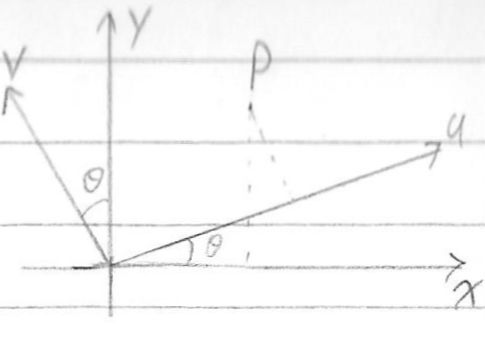
\includegraphics[scale=2]{matrixTransform}
	\caption{Rotation of axes}
	\label{fig:matrixTransform}
	\end{figure}
	
	\textbullet \quad Rotation of axes \linebreak 
	$\displaystyle \begin{pmatrix}
	u \\ v
	\end{pmatrix} = \begin{pmatrix}
	\cos \theta & \sin \theta \\ -\sin \theta & \cos \theta
	\end{pmatrix} \cdot \begin{pmatrix}
	x \\ y
	\end{pmatrix} $ \linebreak 
	$\displaystyle \begin{pmatrix}
	x \\ y
	\end{pmatrix} = \begin{pmatrix}
	\cos \theta & -\sin \theta \\ \sin \theta & \cos \theta
	\end{pmatrix} \cdot \begin{pmatrix}
	u \\ v
	\end{pmatrix} $ \linebreak 
	
	\textbullet \quad \uline{Cayley-Hamilton theorem}: Every square matrix satisfies its own characteristic equation. \linebreak 
	\textbullet \quad \uline{Modal Matrix}: If the $n$ eigenvectors $\textbf{x} _i$ of a square matrix $\textbf{A}$ are arranged as columns, the modal matrix of $\textbf{A}$, denoted by $\textbf{M}$, is formed. i.e. $\displaystyle \textbf{M} = \big( \textbf{x} _1, \textbf{x} _2, \ldots, \textbf{x} _n \big) $. \linebreak 
	\textbullet \quad \uline{Spectral Matrix}: A diagonal matrix with the eigenvalues only on the main diagonal, denoted by $\textbf{S}$. This process is called diagonalisation. \linebreak 
	\textbullet \quad The relationship between $\displaystyle  \textbf{M}$ and $\textbf{S}$ is: $\textbf{M}^{-1} \cdot \textbf{A} \cdot \textbf{M} = \textbf{S}$. \linebreak 
	\textbullet \quad Considering two non-equal matrices $\displaystyle \textbf{A}, \textbf{B}$. If $\textbf{A}\cdot \textbf{B} = \textbf{B} \cdot \textbf{A} $ we say that the two matrices commute. \linebreak 	
	
	\textbullet \quad A square matrix that is not invertible is called \uline{singular}, or degenerate. A square matrix is singular if and only if its determinant is $0$. Singular matrices are rare in the sense that a square matrix randomly selected from a continuous uniform distribution on its entries will almost never be singular. \linebreak 
	\textbullet \quad An orthogonal matrix is a square matrix with real entries whose columns and rows are orthogonal unit vectors (i.e., orthonormal vectors), i.e.: $ \displaystyle Q^T Q = Q Q^T = I $, where $I$ is the identity matrix. This means that a matrix is orthogonal if its transpose is equal to its inverse. \linebreak 
	
	
	\pagebreak
	
	
	\section{Coordinate Systems}
	
	\subsection{2-D Coordinate Systems}	
	
	\textbf{1.} \uline{Cartesian Coordinate System}:	The standard orthogonal $2$-dimentional coordinate system, with $(x,y)$ coordinates. \linebreak 
	
	\textbf{2.} \uline{Polar Coordinate System}: A $2$-dimentional coordinate system $(r,\theta)$ \figref{2dPolarCoordinateSystem} \linebreak 
	where $r = $ radius, $\theta = $ azimuth \linebreak 
	$\displaystyle x = r \cos \theta \ y = r \sin \theta \ r = \sqrt{x^2 +y^2} \ \tan \theta = \frac{y}{x} $ 
	
	\begin{figure}[H]
	\centering
	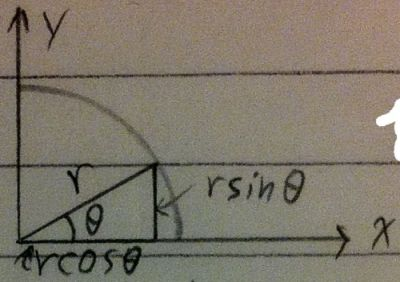
\includegraphics[scale=0.6]{2dPolarCoordinateSystem}
	\caption{Representation of the Polar (planar) Coordinate System}
	\label{fig:2dPolarCoordinateSystem}
	\end{figure}
	
	\subsection{3-D Coordinate Systems}	
		
	\textbf{1.} \uline{Cartesian Coordinates} $(x,y,z)$ (\figref{3dcartesianCoordinateSystem}) \linebreak 
	First octant: $\displaystyle x\geq 0 \ , \ y \geq 0 \ , \ z \geq 0$ \linebreak 	
	
	\begin{figure}[H]
	\centering
	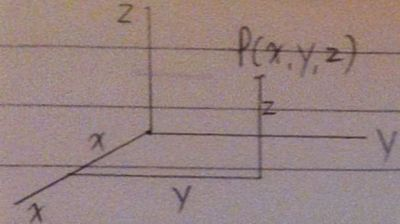
\includegraphics[scale=0.8]{3dcartesianCoordinateSystem}
	\caption{3-Dimensional Coordinate System}
	\label{fig:3dcartesianCoordinateSystem}
	\end{figure}
	
	\textbf{2.} \uline{Cylindrical Coordinates} $(r,\theta, z) \ , \ r \geq 0$ (\figref{cylindricalCoordinateSystem}) \linebreak 
	$\displaystyle x = r \cos \theta \ y = r \sin \theta \ z = z$ \linebreak 
	$\displaystyle r = \sqrt{x^2 +y^2} \ \theta = \tan ^{-1} (\frac{y}{x}) \ z = z$ \linebreak 
	Cylindrical coordinates are useful when an axis of symmetry occurs. \linebreak 
	
	\begin{figure}[H]
	\centering
	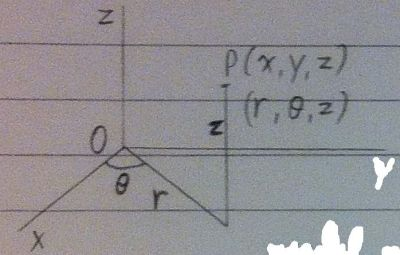
\includegraphics[scale=0.8]{cylindricalCoordinateSystem}
	\caption{Cylidrical Coordinate System}
	\label{fig:cylindricalCoordinateSystem}
	\end{figure}
	
	\textbf{3.} \uline{Spherical Coordinates} $(r,\theta, \phi ) \ , \ r\geq 0$ (\figref{sphericalCoordinateSystem}) \linebreak 
	$\displaystyle x = r \sin \theta \cos \phi \ y = r \sin \theta \sin \phi \ z = r \cos \theta $ \linebreak 
	$\displaystyle r = \sqrt{x^2 +y^2 +z^2} \ \theta = \cos ^{-1} \left(\frac{z}{r}\right) \ \phi = \tan ^{-1} \left( \frac{y}{x} \right)  $ \linebreak 
	Spherical coordinates are useful where a centre of symmetry occurs. \linebreak 
	
	\begin{figure}[H]
	\centering
	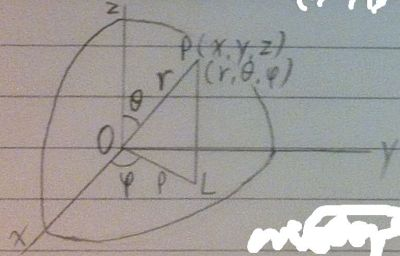
\includegraphics[scale=0.8]{sphericalCoordinateSystem}
	\caption{Spherical Coordinate System}
	\label{fig:sphericalCoordinateSystem}
	\end{figure}
	
	\subsection{Moment of Area}
	
	\uline{Element of Area in Polar Coordinates}: $\delta a = r \delta r \delta \theta $ (\figref{	polarElementOfArea}) \linebreak 
	
	\begin{figure}[H]
	\centering
	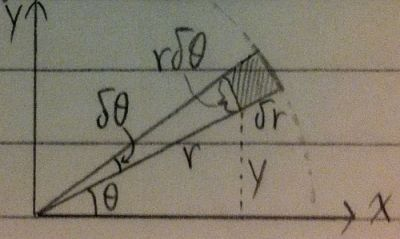
\includegraphics[scale=0.8]{polarElementOfArea}
	\caption{Element of Area in Polar Coordinates}
	\label{fig:polarElementOfArea}
	\end{figure}
	
	\subsection{Element of Volume} 
	
	\textbf{1.} \uline{Cartesian coordinates}: $\displaystyle \delta v = \delta x \delta y \delta z $ \linebreak (\figref{cartesianMomentOfVolume}) \linebreak 
	
	\begin{figure}[H]
	\centering
	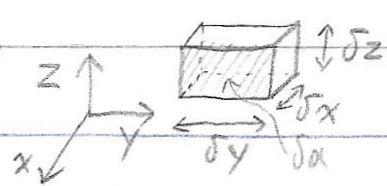
\includegraphics[scale=2]{cartesianMomentOfVolume}
	\caption{Element of Volume in Cartesian Coordinates}
	\label{fig:cartesianMomentOfVolume}
	\end{figure}
	
	\textbf{2.} \uline{Cylindrical coordinates}: $\displaystyle \delta v = r \delta \theta \delta r \delta z = r \delta r \delta \theta \delta z$ \linebreak (\figref{cylindricalMomentOfVolume}) \linebreak 
	
	\begin{figure}[H]
	\centering
	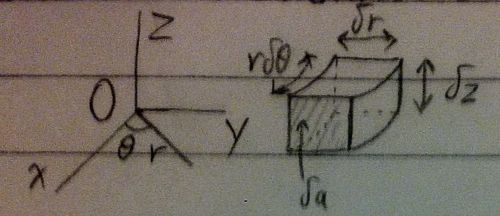
\includegraphics[scale=0.6]{cylindricalMomentOfVolume}
	\caption{Element of Volume in Cylidrical Coordinates}
	\label{fig:cylindricalMomentOfVolume}
	\end{figure}
	
	\textbf{3.} \uline{Spherical coordinates}: $\displaystyle \delta v = \delta v r \delta \theta \ r\sin \phi \delta \phi = r^2 \sin \theta \delta r \delta \theta \delta \phi$ (\figref{sphericalMomentOfVolume}) \linebreak 
	
	\begin{figure}[H]
	\centering
	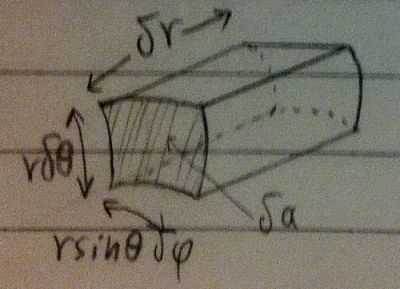
\includegraphics[scale=0.6]{sphericalMomentOfVolume}
	\caption{Element of Volume in Spherical Coordinates}
	\label{fig:sphericalMomentOfVolume}
	\end{figure}
	
	[$\delta a = \text{hedra}$] \linebreak 

	\subsection{Element of Area in Space} 
	
	\textbf{1.} Cartesian coordinates: $\displaystyle \delta a = \delta x \delta y$ \linebreak 
	\textbf{2.} Cylindrical coordinates: $\displaystyle \delta a = r \delta \theta \delta z $ \linebreak 
	\textbf{3.} Spherical coordinates: $\displaystyle \delta a = r^2 \sin \theta \delta \theta \delta \phi $ \linebreak 
	
	\subsection{Curvilinear Coordinates}	
	
	\textbullet \quad Curvilinear coordinates is a coordinate system for Euclidean space in which the coordinate lines may be curves, as well as the coordinate surfaces. These coordinates may be derived from a set of Cartesian coordinates by using a transformation that is locally invertible (a one-to-one map) at each point. As such, in the general case (3D): $u = f(x,y,z) \ , \ v = g(x,y,z,) \ , \ w = h (x,y,z)$ \linebreak 
	\textbullet \quad If the coordinate curves for $u$ and $v$ forming the network cross at right angles, the system of coordinates is said to be \uline{orthogonal}. That is, if $\displaystyle \frac{\partial u}{\partial x} \cdot \frac{\partial v}{\partial x} + \frac{\partial u}{\partial y} \cdot \frac{\partial v}{\partial y} = 0$  then $u$ and $v$ are orthogonal. \linebreak 
	
	\textbullet \quad \uline{Orthogonal Coordinate system in space (Curvilinear)} \linebreak 
	\textbf{a}) Cartesian Rectangular Coordinates $(x,y,z)$ \linebreak 
	$\displaystyle \vec{F} = F_x \vec{i} + F_y \vec{j} + F_z \vec{k} $ , Scale factors: $h_x = h_y = h_z = 1$ \linebreak 
	\textbf{b}) Cylindrical Polar Coordinates $(r,\theta, z)$ \linebreak 
	$\displaystyle \vec{r} = r \cos \theta \vec{i} + r \sin \theta \vec{j} + z\vec{k}$ \linebreak 
	
	\textbf{Base unit vectors} \linebreak 
	$\displaystyle \vec{I} = \frac{\partial \vec{r}}{\partial r} \big/ \left| \frac{\partial \vec{r}}{\partial r} \right| $ \linebreak 
	$\displaystyle \vec{J} = \frac{\partial \vec{r}}{\partial \theta} \big/ \left| \frac{\partial \vec{r}}{\partial \theta} \right| $ \linebreak 
	$\displaystyle \vec{K} = \frac{\partial \vec{r}}{\partial z} \big/ \left| \frac{\partial \vec{r}}{\partial z} \right| $ \linebreak 

	\textbf{Scale factors} \linebreak 
	$\displaystyle h_r = \left| \frac{\partial \vec{r}}{\partial r} \right| = 1$ \linebreak 
	$\displaystyle h_{\theta} = \left| \frac{\partial \vec{r}}{\partial \theta} \right| = r$ \linebreak 
	$\displaystyle h_z = \left| \frac{\partial \vec{r}}{\partial z} \right| = 1$ \linebreak 
	
	$$ \vec{F} = F_r \vec{I} + F_{\theta} \vec{J} + F_z \vec{K} $$
	
	\textbf{c}) Spherical Polar Coordinates $(r,\theta, \phi)$ \linebreak 
	$\displaystyle \vec{r} = r \sin \theta \cos \phi \vec{i} + r \sin \theta \sin \phi \vec{j} + r \cos \theta \vec{k}$ \linebreak 
	
	\textbf{Base unit vectors} \linebreak 
	$\displaystyle \vec{I} = \frac{\partial \vec{r}}{\partial r} \big/ \left| \frac{\partial \vec{r}}{\partial r} \right| $ \linebreak 
	$\displaystyle \vec{J} = \frac{\partial \vec{r}}{\partial \theta} \big/ \left| \frac{\partial \vec{r}}{\partial \theta} \right| $ \linebreak 
	$\displaystyle \vec{K} = \frac{\partial \vec{r}}{\partial \phi} \big/ \left| \frac{\partial \vec{r}}{\partial \phi} \right| $ \linebreak 

	\textbf{Scale factors} \linebreak 
	$\displaystyle h_r = \left| \frac{\partial \vec{r}}{\partial r} \right| = 1 $ \linebreak 
	$\displaystyle h_{\theta} = \left| \frac{\partial \vec{r}}{\partial \theta} \right| = r $ \linebreak 
	$\displaystyle h_{\phi} = \left| \frac{\partial \vec{r}}{\partial \phi} \right| = r\sin \theta $ \linebreak 
	
	$$ \vec{F} = F_r \vec{I} + F_{\theta} \vec{J} + F_{\phi} \vec{K} $$
	
	\textbullet \quad \uline{General Orthogonal Curvilinear coordinates $(u,v,w)$} \linebreak 
	$\displaystyle x = f(u,v,w) \ , \ y = g(u,v,w) \ , \ z = h(u,v,w) $ \linebreak 
	$\displaystyle \vec{r} = x \vec{i} + y \vec{j} + z \vec{k} $ \linebreak 
	$\displaystyle \frac{\partial \vec{r}}{\partial u} = h_u \vec{I} \ $, where $\displaystyle h_u = \left| \frac{\partial \vec{r}}{\partial u} \right| $ \linebreak 
	$\displaystyle \left| \frac{\partial \vec{r}}{\partial v} \right| = h_v \vec{J} \ $, where $\displaystyle h_v = \left| \frac{\partial \vec{r}}{\partial v} \right| $ \linebreak 
	$\displaystyle \left| \frac{\partial \vec{r}}{\partial w} \right| = h_w \vec{K} \ $, where $\displaystyle h_w = \left| \frac{\partial \vec{r}}{\partial w} \right| $ \linebreak 
	
	\textbullet \quad Element of arc: $\displaystyle ds = \left( h_u^2 du^2 + h_v^2 dv^2 + h_w^2 dw^2 \right)^{\frac{1}{2}} $ \linebreak 
	\textbullet \quad Element of volume: $\displaystyle dV = h_uh_vh_w dudvdw = \frac{\partial (x,y,z)}{\partial (u,v,w)} dudvdw $ \linebreak 
	
	
	\pagebreak
	
	
	\section{Transforms} 
	
	\subsection{Laplace Transforms}
	
	\textbullet \quad $\displaystyle \mathcal{L} \{ f(t) \} = \int_{t=0}^{\infty} e^{-st} f(t) dt = F(s) $  :  Definition (\uline{single sided}) \linebreak 
	where $\displaystyle e^{-st}f(t)$ must converge as $\displaystyle t\to \infty \ , \ s=\sigma +j\omega \text{complex frequency} \ , \sigma >0$ \linebreak 	
	and $f(t)$ is a continuous, or piecewise continuous, function. \linebreak 
	\textbullet \quad $\displaystyle f(t) = \mathcal{L}^{-1} \{ F(s) \} $  :  Inverse Laplace transform \linebreak 
	\textbullet \quad $s= \sigma + j\omega$  :  Complex frequency. $\sigma$  :  represents the  transient component, $\omega$  :  represents the steady state component \linebreak 
	\uline{Properties} \linebreak 
	\textbullet \quad Both the LaPlace transform and its inverse are linear transforms. This means that:  
	\begin{enumerate}
	\item $\displaystyle \mathcal{L} \{f(t) \pm g(t) \} = \mathcal{L} \{ f(t) \} \pm \mathcal{L} \{ g(t) \} $ \linebreak 
			$\displaystyle \mathcal{L}^{-1} \{ F(s) \pm G(s) \} = \mathcal{L}^{-1} \{ F(s) \} \pm \mathcal{L}^{-1} G(s) \}$
	\item $\displaystyle \mathcal{L} \{ kf(t) \} = k \mathcal{L} \{ f(t) \} $ \linebreak 
			$\displaystyle \mathcal{L}^{-1} \{kF(s) \} = k\mathcal{L}^{-1} \{ F(s) \} $ 
	\item Laplacian of a derivative: $\displaystyle \mathcal{L} \{ f'(t) \} = sF(s) - f(0) $
	\item Laplacian of higher derivatives: \linebreak 
			$\displaystyle \mathcal{L} \{ f^{(\nu)} (t) \} = s^{\nu} F(s) - s^{\nu -1} f(0) - s^{\nu -2} f'(0) - s^{\nu -3} f''(0) - \ldots - f^{(\nu -1)} (0)$ 
	\item $\displaystyle ^{(\nu)} (s) = (-1)^n \mathcal{L} \{ t^n f(t) \} $ 
	\item $\displaystyle F(s-k) = \mathcal{L} \{ e^{kt} f(t) \} $ 
	\item $\displaystyle \mathcal{L} \{ e^{-at} f(t) \} = F(s+a) $ (1st Shift Theorem) 
	\item $\displaystyle \displaystyle \mathcal{L} \{ t^n f(t) \} = (-1)^n \frac{d^n}{ds^n} \left(F(s)\right) $ (Multiplication by $t^n$) 
	\item $\displaystyle \mathcal{L} \{ \frac{f(t)}{t} \} = \int_{\sigma = s}^{\infty} F(\sigma) d\sigma$, provided that $\exists \lim_{t\to 0} \left( \frac{f(t)}{t} \right) $ 
	\item $\displaystyle \mathcal{L} \{u(t-c) \cdot f(t-c) \} = e^{-cs} F(s)\ , \ c\in \mathbb{R} $  :  2nd Shift Theorem, where $F(s) = \mathcal{L} \{ f(t) \}$
	\item $\displaystyle \mathcal{L} \{ f(t) \ast g(t) \} = F(s) \cdot G(s) = \mathcal{L} \{ f(t) \} \cdot \mathcal{L} \{ g(t) \}$  :  Convolution theorem 
	\item $\displaystyle \mathcal{L} \big\{ \overset{-}{f} (t) \big\} = \frac{1}{1-e^{-s\Tau}} F(s) $ \linebreak 
	where $\displaystyle F(s) = \int_{0\ ( \text{or} -\Tau / 2)}^{\Tau ( \text{or} \Tau / 2)} e^{-st} f(t) dt$ \linebreak 
	$\displaystyle \overset{-}{f} (t)$ is a periodic function, with period $\Tau$. 
	\item $\displaystyle \mathcal{L} \{ f(t) \cdot \delta (t-c) \} = f(c) e^{-cs} $ 
	\item To find inverse transforms involving periodic functions, expand the $\displaystyle (1-e^{-cs})$ term in the denominator as the binomial series: $\displaystyle (1-x)^{-1} = 1 +x + x^2 + x^3 + \ldots$ 
	\item $\displaystyle \int_0^t f(\tau) d\tau \leftrightarrow \frac{F(s)}{s}$ 
	\item $\displaystyle f(t) \cdot g(t) \leftrightarrow F(s) \ast G(s) $ 
	\item $\displaystyle f(\frac{t}{a}) u(t) \leftrightarrow aF(as) \ , \ \forall a\in \mathbb{R}^+ $ 
	\item $\displaystyle f(\frac{t}{a} -b) u(t) \leftrightarrow ae^{-sab} F(as) \ , \ \forall a\in \mathbb{R}^+ $ 
	\item $\displaystyle f(0_+) = \lim_{s\to \infty} \left[ sF(s) \right] $  :  Initial Value Theorem, where $f(t)$ is a one-sided function 
	\item $\displaystyle \lim_{t\to \infty } \left[ f(t) \right] = \lim_{s \to 0} \left[ sF(s) \right] $  :  Final Value theorem, \linebreak 
	provided that the $\displaystyle \lim_{t\to \infty} \left[ f(t) \right] $ exists, i.e. $f(t)$ has a final value. 
	\end{enumerate} 
	
	\textbullet \quad Using the LaPlace transform we can solve equations of the form: $\displaystyle a_n f^{(n)} (t) + a_{n-1} f^{(n-1)} (t) + \ldots a_2 f''(t) + a_1 f'(t) + a_0 f(t) = g(t) $, where $\displaystyle a_n, a_{n-1}, \ldots, a_2, a_1, a_0$ are known constants, $g(t)$ is a known expression of $t$ and the values of $f(t)$ and its derivatives are known at $t=0$. \linebreak 
	This type of equation is called a linear, constant-coefficient, inhomogeneous differential equation and the values of $f(t)$ and its derivatives are called boundary conditions. The method to find the solution is: \linebreak 
	a) Take the LaPlace Transform of both sides. \linebreak 
	b) Find the expression $\displaystyle F(s) = \mathcal{L} \{ f(t) \} $ in the form of an algebraic fraction. \linebreak 
	c) Separate $F(s)$ into its partial fractions. \linebreak 
	d) Find $\displaystyle \mathcal{L}^{-1} \{ F(s) \}$ to find the solution $f(t)$. \linebreak 
	
	\uline{Table of LaPlace Transforms} \linebreak 
	$$ \begin{bmatrix}
	f(t) & \mathcal{L} \{ f(t) \} = F(s) \\ 
	a & \frac{a}{s} \ \ , \ s>0 \\
	e^{-at} u(t) & \frac{1}{s+a} \ \ , \ s > -a \\ 
	t^n u(t) & \frac{n!}{s^{n+1}} \ \ , \ n\in \mathbb{N}^* \\ 
	\sin (at) \cdot u(t) & \frac{a}{s^2 + a^2} \ \ , \ s> 0 \\ 
	\cos (at) \cdot u(t) & \frac{s}{s^2 +a^2} \ \ , \ s>0 \\
	\sinh (at) \cdot u(t) & \frac{a}{s^2-a^2} \ \ , \ s> |a| \\ 
	\cosh (at) \cdot u(t) & \frac{s}{s^2-a^2} \ \ , \ s> |a| \\ 
	u(t-c) & \frac{e^{-cs}}{s} \\ 
	\delta(t-c) & e^{-cs} \\ 
	\ln \left(\frac{t}{\Tau} \right) u(t) & -\frac{\Tau}{s} \big| \ln (\Tau s) + \gamma \big| \\ 
	f(t) \sin (ct) u(t) & \frac{1}{2j} \left[ F(s-jc) - F(s+jc) \right] \\ 
	f(t) \cos (ct) u(t) & \frac{1}{2} \left[ F(s-jc) + F(s+jc) \right] \\ 
	a^{ct} \cdot u(t) & \frac{1}{s-c \ln(a)} \ , \ s>c\\ln(a) \\ 
	r(t-T) = (t-T) u(t-T) & \frac{1}{s^2} \cdot e^{-Ts} 
	\end{bmatrix} $$
	\linebreak 
	
	\subsubsection{Convolution} 
	
	\textbullet \quad $\displaystyle c(t) = f(t) \Conv g(t) = \int_{-\infty}^{\infty} f(x) g(t-x) dx $     (flip and slide) \linebreak 
	
	\uline{Properties} 
	\begin{enumerate}
	\item $\displaystyle f(t) \Conv h(t) = h(t) \Conv f(t)$ 
	\item $\displaystyle \left[ f(t) \Conv h(t) \right] \Conv c(t) = f(t) \Conv \left[ h(t) \Conv c(t) \right] $ 
	\item $\displaystyle f(t) \Conv \left[ h(t) + c(t) \right] = f(t) \Conv h(t) + f(t) \Conv c(t) $ 
	\item $\displaystyle f(t) \Conv \delta (t) = f(t) $ 
	\item $\displaystyle f(t) \Conv \delta (t-t_0)) = f(t-t_0) $ 		
	\end{enumerate}  
	
	\textbullet \quad The convolution of two functions $x(t)$, $h(t)$ is obtained by: 
	\begin{enumerate}
	\item Changing variable $t$ to the dummy variable $T$. 
	\item Reversing one of them, say $h(T)$ to form $h(-T$ [if it isn't already in the form $h(-T)$].
	\item Shifting $h(-T)$ by $t$ units to the left, $h(t-T)$. 
	\item Taking the product of $x(t)$ and $h(t-T)$ and integrating with respect to $T$.  
	\quad \quad $\displaystyle t \Rightarrow T \Rightarrow t \Rightarrow T$ 
	\end{enumerate} 
	
	\subsection{Z Transform}
	
	\textbullet \quad $\displaystyle Z\left\{ f[n] \right\} = F(z) = \sum \limits_{n= -\infty}^{\infty} f[n] z^{-n} \ , \ n\in \mathbb{Z} $  :  Definition (bilateral) \linebreak 
	$\displaystyle f[n] \left( =f(n) \right)$ is a discrete function. \linebreak 
	
	\uline{Properties}  
	\begin{enumerate}
	\item $\displaystyle Z\{af[n] + bg[n] \} = aZ \{ f[n] \} + bZ \{ g[n] \} $  :  Linearity 
	\item $\displaystyle F(z) = Z\{f[n] \} \rightarrow Z \{f[n+m] \} = z^m F(z) - \left[ z^m f[0] + z^{m-1} f[1] + \ldots + zf[m-1] \right]$  :  Shifting Left 
	\item $\displaystyle F(z) = Z\{ f[n] \} \rightarrow Z\{ f[n-m] \} = z^{-m} F(z)$  :  Shifting Right 
	\item $\displaystyle F(z) = Z \{f[n] \} \rightarrow Z \{ a^n f[n] \} = F\left( \frac{z}{a} \right) $  :  Translation 
	\item $\displaystyle \lim_{n\to \infty} f[n] = \lim_{z \to 1} \big\{ \left( \frac{z-1}{z} \right) F(z) \big\} $  :  Final Value Theorem, provided that $\displaystyle \lim_{n\to \infty} f[n]$ exists. 
	\item $\displaystyle f(0) = \lim_{z\to \infty} \left\{ F(z) \right\} $  :  Initial Value Theorem 
	\item $\displaystyle F(z) = Z\left\{ f[n] \right\} \rightarrow Z \left\{ nf[n] \right\} = -z F' (z) $  :  Derivative of the transform 
	\end{enumerate} 
	
	\uline{Table of Z Transforms} \linebreak 
	$$ \begin{bmatrix}
	f[n] & F(z) \ \  R.O.C. \\ 
	\delta[n] & 1 \\ 
	u[n] & \frac{z}{z-1} \ , \ |z| > 1 \\ 
	nu[n] &  \frac{z}{(z-1)^2} \ , \ |z| > 1 \\ 
	n^2u[n] & \frac{z(z+1)}{(z-1)^3} \ , \ |z| > 1 \\ 
	n^3u[n] & \frac{z(z^2+4z+1)}{(z-1)^4} \ , \ |z| > 1 \\ 
	a^n u[n] & \frac{z}{z-a} \ , \ |z| > |a| \\ 
	na^n u[n] & \frac{az}{(z-a)^2} \ , \ |z| > |a| \\ 
	\delta [n-c] & z^{-cn} \\ 
	e^{-an} \cdot u[n] & \frac{z}{z-e^{-a}} \ , \ |z| > e^{-a}  \\ 
	\sin [an] \cdot u[n] & \frac{\sin (a) \cdot z}{z^2 -2\cos (a) \cdot z + 1} \ , \ |z| > 1 \\ 
	b^n \sin [an] \cdot u[n] & \frac{b\sin (a) \cdot z}{z^2 -2b \cos (a) \cdot z +b^2} \ , \ |z| > b \\ 
	\cos [an] \cdot u[n] & \frac{z(z-\cos (a))}{z^2 -2 \cos (a) \cdot z + 1} \ , \ |z| > 1 \\ 
	b^n \cdot \cos [an] \cdot u[n] & \frac{z(z-b\cos (a))}{z^2 -2b \cos (a) \cdot z + b^2} \ , \ |z| > b \\
	C u[n] \ , \ C \in \mathbb{C} & \frac{Cz}{z-1} \ , \ |z| > 1 
	\end{bmatrix} $$
	
	\subsubsection{Sampling} 
	
	If a continuous function $f(t)$ is sampled at equal intervals, the resulting sequence has a $Z$ transform that is related to the Laplace transform of the piecewise function created $f^*(t)$ from the sequence of sampled values. \linebreak 
	$\displaystyle \mathcal{L} \left\{ f^*(t) \right\} = \sum \limits_{k=0}^{\infty} f(kT) z^{-k} = Z \left\{ f(kT) \right\}$ \linebreak 
	where $\displaystyle \left\{ f(kT) \right\} = \left\{ f(0), f(T), f(2T), f(3T), \ldots \right\} $ \linebreak 
	$\displaystyle f^* (t) = 	\begin{cases} 
											f(kT) \ , & \text{if} \ t=k \ , \ \text{and} \ z=e^{sT} \\ 
											0 \ , & \text{otherwise} 
										\end{cases} $ \linebreak 
	
	\subsection{Fourier Transform}
	
	\textbullet \quad \uline{Definition}: If \linebreak 
	$(a) f(t)$ and $f'(t)$ are piecewise continuous in every finite interval, and 
	$(b) f(t)$ is absolutely integrable in $(-\infty, \infty )$, that is $\int_{-\infty}^{\infty} |f(t)| dt$ is finite, then \linebreak 
	$\displaystyle (\rightarrow) F(\omega) = \int_{-\infty}^{\infty} f(t) e^{-j\omega t} dt = \mathcal{F} \left\{ f(t) \right\}$ (or $f(t)$'s spectrum) \& $\displaystyle (\leftarrow) \ f(t) = \int_{-\infty}^{\infty} F(\omega) e^{j\omega t} d\omega = \mathcal{F}^{-1} \{ F(\omega)\}$ \linebreak 
	\textbullet \quad The Fourier transform $F(\omega)$ is a complex function, so $\displaystyle F(\omega) = \left| F(\omega) \right| e^{j\phi (\omega)}$, where $\displaystyle \left| F(\omega) \right|$ is the continuous amplitude spectrum and $\phi (\omega)$ is the continuous phase spectrum. \linebreak 
	\textbullet \quad The Fourier transform describes a waveform $f(t)$ into the frequency domain, just like the complex $c_n$ coefficients of f.s. for periodic signals. \linebreak 
	
	\uline{Properties}  
	\begin{enumerate}
	\item Fourier cosine transformation: $f(t)$ even function $\displaystyle \leftrightarrow F(\omega) = \int_{-\infty}^{\infty} f(t) \cos (\omega t) dt \ \in \mathbb{R}\text{e}$ 
	\item Fourier sine transformation: $f(t)$ odd function $\displaystyle \leftrightarrow F(\omega) = j \int_{-\infty}^{\infty} f(t) \sin (\omega t) dt \in \mathbb{I}\text{m} = 2j \int_0^{\infty} f(t) \sin (\omega t) dt \in \mathbb{I}\text{m}$ \linebreak 
	\item Linearity: $\displaystyle \mathcal{F} \{a_1 f_1(t) + a_2 f_2 (t) \} = a_1 F_1(\omega) + a_2 F_2(\omega) $ 
	\item Time shifting: $\displaystyle \mathcal{f(t)} = F(\omega) \rightarrow \mathcal{F} \{f(t-t_0) \} = e^{j\omega t_0} F(\omega)$ 
	\item Frequency shifting: $\displaystyle \mathcal{F} \{ f(t) \} = F(\omega) \rightarrow \mathcal{F} \{ f(kt) \} = \frac{1}{|k|} F\left( \frac{\omega}{k} \right) $ 
	\item Symmetry: $\displaystyle \mathcal{F} \{ f(t) \} = F(\omega) \rightarrow \mathcal{F} \{ F(\omega) \} = f(-\omega) $
	\item Differentiation: $\displaystyle \mathcal{F} \{ f(t) \} = F(\omega) \rightarrow \mathcal{F} \left\{ \frac{d^n}{dt^n} f(t) \right\} = (n\omega)^n F(\omega) $ 
	\item Convolution property: $\displaystyle \big[ \mathcal{F} \{f(t) \} = F(\omega) \land \mathcal{F}\{ g(t) \} = G(\omega) \big] \rightarrow \big[ \mathcal{F} \{ f(t) \Conv g(t) \} = F(\omega) \cdot G(\omega) \big] $ 
	\item Integration: $\displaystyle \mathcal{F} \big[ \int_{-\infty}^t \chi (\tau) d \tau \big] = \frac{\Chi (\omega}{j\omega} + \frac{1}{2} \Chi(0) \delta (\omega) $ 
	\item The Fourier transform of a real signal is a Hermitian function. 
	\item Rayleigh Energy Theorem: $\displaystyle E = \int_{-\infty}^{\infty} | x(t)|^2 dt = \int_{-\infty}^{\infty} |X(\omega)|^2 d\omega$ 
	\end{enumerate} 
	
	\uline{Fourier Transform Table} \linebreak 
	$$ \begin{bmatrix}
	f(t) & F(\omega) \ (\omega = 2\pi f) \\ 
	\delta(t) & 1 \\ 
	1 & \delta(\omega) \\ 
	\delta (t-t_0) & e^{-j\omega t_0} \\ 
	e^{j\omega_0 t} & \delta (\omega - \omega_0) \\ 
	\cos (\omega_0 t)  &  \frac{1}{2} \delta(\omega - \omega_0) + \frac{1}{2} \delta (\omega + \omega_0)  \\ 
	\sin (\omega_0 t)  &  \frac{-1}{2j} \delta(\omega + \omega_0) + \frac{1}{2j} \delta (\omega + \omega_0)  \\ 
	\Pi(t) & \sinc (\omega) \\ 
	A \sinc (2\omega_0 t) & (\frac{A}{2\omega_0} \cdot \Pi (\frac{\omega}{2\omega_0} \\ 
	\frac{1}{t}  & -j \pi \cdot \sgn(\omega) \\ 
	\sinc^2(t) &  \Lambda (\omega) \\ 
	u(t) & \frac{1}{2} \delta (\omega) + \frac{1}{j\omega}  \\ 
	e^{-at} u(t) \ , \ a>0 & \frac{1}{j\omega + a} \\ 
	te^{-at} u(t) \ , \ a>0 & \frac{1}{(j\omega + a)^2} \\ 
	e^{-a|t|}  & \frac{2a}{\omega^2 + a} \\ 
	e^{-\pi t^2} & e^{-\pi \omega^2} \\ 
	\Pi_{\alpha} (t) = \begin{cases} 1/\alpha \ , & \frac{-a}{2} < t < \frac{a}{2} \\ 0 \ , & otherwise \end{cases}  & \sinc\left( \frac{\omega a}{2} \right)  \\
	\Lambda(t) = \begin{cases} t+1 \ , & -1 \leq t < 0 \\ 1-t \ , & 0 \leq t < 1 \\ 0 \ , \text{otherwise} \end{cases} & \sinc^2(\omega) \\
	R_X (t_1, t_2) &  S_X(\omega) \\ 
	R_XY (t_1, t_2)  & S_XY (\omega) \\ 
	e^{-\alpha t} \cos (\omega_0 t) u(t) \ , \ a>0 & \frac{a+j\omega}{\omega_0^2 + (a+j\omega^2)^2}  \\ 
	e^{-\alpha t} \sin (\omega_0 t) u(t) \ , \ a>0 & \frac{\omega_0}{\omega_0^2 + (\alpha + j\omega)^2}  \\ 
	\cos (\omega_0 t) u(t) & \frac{j\omega}{\omega_0^2 - \omega^2} + \frac{\pi}{2} \big[ \delta(\omega + \omega_0 + \delta ( \omega - \omega_0) \big]  \\
	\sin (\omega_0 t) u(t) & \frac{\omega_0}{\omega_0^2 -\omega^2} + j\frac{\pi}{2} \big[ \delta(\omega + \omega_0) - \delta (\omega - \omega_0) \big]  
	\end{bmatrix} $$
	
	
	\pagebreak	
	
	
	\section{Special Functions}
	
	\uline{Heaviside unit step function}: $f(t) = u(t-c) \begin{cases} 0 & t < c \\ 1 & t > c \end{cases}$ \linebreak 
	Properties \linebreak 
	\textbullet \quad $u(t) + u(-t) = 1$ \linebreak 
	
	\uline{Ramp function}: $r(t-c) = \begin{cases} t & t > c \\ 0 & t < c \end{cases}$ \linebreak 
	Properties \linebreak 
	\textbullet \quad $r(t) = \int_{-\infty}^t u(\tau) d\tau	$ \linebreak 
	\textbullet \quad $r(t-c) = tu(t-c) $ \linebreak 
	\textbullet \quad $r(t-c) = (t-c) u(t-c) $ \linebreak 
	\textbullet \quad $\displaystyle \frac{d}{dt} r(t) = u(t) $ \linebreak 
	\textbullet \quad $\displaystyle \frac{d}{dt} \left( r(t-c) \right) = (t-c) u(t-c) $ \linebreak 
	
	\uline{Signum Function}: $ \sgn (t) =  \begin{cases} 1 & t>0 \\ -1 & t < 0 \\ 0 & t = 0 \end{cases} $ \linebreak 
	Properties \linebreak 
	\textbullet \quad $\forall x \in \mathbb{R} ( x= \sgn (x) \cdot |x| ) $ \linebreak 
	\textbullet \quad $ \sgn (x) = \frac{x}{|x|} = \frac{|x|}{x} $ \linebreak 
	\textbullet \quad $ \frac{d|x|}{dx} = \sgn (x) $ \linebreak 
	\textbullet \quad $ \sgn (t) + 1 = 2u(t) $ \linebreak 
	\textbullet \quad $ \sgn (t) = u(t) - u(-t) $ \linebreak 
	
	\uline{Unit Impulse / Dirac Delta}: $\delta(t)$ \linebreak 
	$\displaystyle \int_{-\infty}^{\infty} f(t) \delta (t-a) dt = f(a) $ , where $f(t)$ is a continuous function @$t=a \ , a\in \mathbb{R} $ \linebreak 
	\textbullet \quad In function terms: $\delta (t) = \begin{cases} 0 & t \neq 0 \\ \text{undefined} & t=0 \end{cases} $ \linebreak 
	Properties \linebreak 
	\textbullet \quad $\displaystyle \int_{-\infty}^{\infty} \delta (t-a) dt = 1 $ \linebreak 
	\textbullet \quad $\displaystyle \int_p^q \delta (t-a) = 1 \ , p < a < q $ \linebreak 
	\textbullet \quad $u(t) = \int_{-\infty}^t \delta(\tau) d\tau $ \linebreak 
	\textbullet \quad $\frac{d}{dt} u(t) = \delta (t) $ \linebreak 
	\textbullet \quad $ \delta'(t) = \frac{d}{dt} \delta (t) $  :  Unit doublet \linebreak 
	\textbullet \quad $\delta (t) = \delta (-t) \ , \ \delta(t-\tau) = \delta (\tau - t) \ $ (Even) \linebreak 
	\textbullet \quad $f(t) \delta (t-c) = f(c) \delta (t-c) \ , \ f(t)$  :  continuous function at $t=c$  :  Sampling property \linebreak 
	\textbullet \quad $\displaystyle f(t) = \int_{-\infty}^{\infty} f(\tau) \delta (t-\tau) d\tau $  :  Construction of $f(t)$ by the sum of all its samples $\Tau$, or, for discrete functions: $x[n] = \sum \limits{k=-\infty}^{\infty} x[k] \delta[n-k]$ \linebreak 
	\textbullet \quad $\delta (-t) = \delta (t)$ \linebreak 
	
	\uline{Sinc function}: $ \sinc(x) = \frac{\sin (\pi x)}{\pi x} \ , \ \sinc (0) = 1$ \linebreak 
	Properties \linebreak 
	\textbullet \quad $\sinc (x) = \sinc (-x) $  :  Even function \linebreak 
	\textbullet \quad $\sinc (n) = 0 $ , $ n \in \mathbb{Z}^* $ \linebreak 
	\textbullet \quad $\displaystyle \int_{-\infty}^{\infty} \sinc (x) dx = 1$ \linebreak 
	$\therefore \int_{-\infty}^0 \sinc (x) dx = \int_0^{\infty} \sinc (x) dx = \frac{1}{2} $ \linebreak 
	
	\uline{Sine Integral}: $\displaystyle Si(t) = \int_0^t \frac{\sin (x)}{x} dx $ \linebreak 
	Properties \linebreak 
	\textbullet \quad $Si(0) = 0$ \linebreak 
	\textbullet \quad $\lim_{t\to \infty} Si(t) = Si(\infty) = \frac{\pi}{2} = \int_0^{\infty} \frac{\sin (x)}{x} dx$ \linebreak 
	\textbullet \quad $\int_0^t \sinc (x) dx = \frac{Si(\pi t)}{\pi} $ \linebreak 
	\textbullet \quad $ \frac{d}{dx} \big[ \frac{Si(\pi x)}{\pi} \big] = \sinc (x) $ \linebreak 
	
	\uline{Periodic Functions} \linebreak 
	$\displaystyle \overset{-}{f}(t) = f(t) + f(t-T) + f(t-2T) + f(t-3T) + \ldots + f(t-nT) \ , \ n\in \mathbb{Z} \ , \ T \in \mathbb{N} $ , with $f(t) = f(t-T) = f(t-2T) = \ldots = f(t-nT)$ \linebreak 
	
	\uline{Orthogonal Functions}: If two different functions $f(x)$ and $g(x)$ are defined on the interval $a\leq x \leq b$ and $\displaystyle \int_a^b f(x) \cdot g(x) dx = 0 $ , then the two functions are orthogonal to each other on the aforementioned interval. \linebreak 
	
	\uline{Kronecker delta function}: $\displaystyle \delta (i,j) = \delta_{ij} = \begin{cases} 1 & i = j \\ 0 & i\neq j \end{cases} $ \linebreak 
	
	\uline{Boxcar function}: $\displaystyle \Pi_w (t-c) = \boxcar \frac{t-c}{w} = \begin{cases} 1 & c-w < t < c+w \\ 1/2 & (t=c+w) \lor (t=c-w) \\ 0 & (t<c-w) \lor (t>c+w) \end{cases} $ 
	\linebreak 
	
	\uline{Rectangular / Top-hat function}: Boxcar function centered at origin ($c=0$): 
	$\displaystyle \rect (\frac{t}{w}) = \Pi ( \frac{t}{w} ) = \begin{cases} 1 & |t| < w/2 \\ 1/2 & |t| = w/2 \\ 0 & otherwise \end{cases} = w\Pi (t) = \Pi_w (t)$ 
	\linebreak 
	Properties \linebreak 
	\textbullet \quad Unit area \linebreak 
	\textbullet \quad $\displaystyle \int_{-\infty}^{\infty} \lim_{w\to 0} \left\{ \Pi_w (t) \right\} dt = \int_{-\infty}^{\infty} \delta (t) dt = 1 $ \linebreak 
	
	\textbullet \quad \uline{Triangle function}: $\displaystyle \Lambda_w (t) = \tri (t) = \Lambda (t) = 
	\begin{cases} 
		\frac{w+t}{w^2} & -w < t < 0 \\ 
		\frac{w-t}{w^2} & 0 < t < w \\ 
		0 & |t| < w 
	\end{cases} $ \linebreak 
	Properties \linebreak 
	
	\begin{figure}[H]
	\centering
	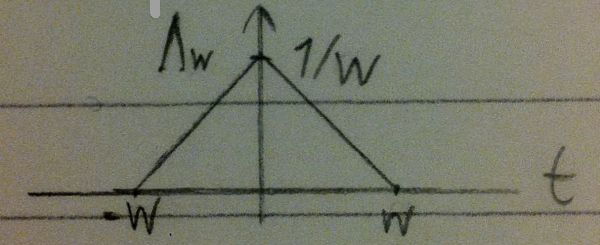
\includegraphics[scale=0.4]{triangleFunction}
	\caption{Triangle Function}
	\label{fig:triangleFunction}
	\end{figure}
	
	\uline{Bessel's equation \& Bessel functions} \linebreak 
	\textbullet \quad Equation: $x^2y'' + xy' + (x^2 -v^2) = 0$ , $v$ is a real constant. \linebreak 
	If we express its two solutions in terms of gamma functions, we obtain the \uline{Bessel function of the 1st kind} of order $v$ - provided $v$ is not a negative integer: \linebreak 
	$\displaystyle J_v (x) = \left(\frac{x}{2} \right)^2 \left\{ \frac{1}{\Gamma (v+1)} - \frac{x^2}{2^2 \cdot 1! \Gamma (v+2)} + \frac{x^4}{2^4 \cdot 2! \cdot \Gamma (v+3) - \ldots} \right\} $ \textbullet \quad 
	Also, $\displaystyle J_{-v} (x) = \left( \frac{x}{2} \right)^{-v} \left\{ \frac{1}{\Gamma (1-v)} - \frac{x^2}{2 \cdot 1! \cdot \Gamma (2-v)} + \frac{x^4}{2^2 \cdot 2! \cdot \Gamma (3-v)} - \ldots \right\} $ \linebreak 
	provided that $v$ is not a positive integer. \linebreak 
	Therefore, complete solution is: $y=A \cdot J_v (x) + B\cdot J_{-v} (x) $ \linebreak 
	When $v=n \in \mathbb{Z}$ , then: $\displaystyle J_n (x) = \left( \frac{x}{2} \right)^n \left\{ \frac{1}{n!} - \frac{1}{(n+1)!} \cdot \left( \frac{x}{2} \right)^2 + \frac{1}{2! \cdot (n+2)!} \left( \frac{x}{2} \right)^4 - \frac{1}{3! \cdot (n+3)!} \left( \frac{x}{2} \right)^6 + \ldots \right\} $ \linebreak 
	
	\uline{Legendre's Equation}: $\displaystyle (1-x^2)y'' -2xy' +k(k+1)y =0$, \linebreak 
	where $k \in \mathbb{R}$ a constant. Solution by Frobenius gives: \linebreak 
	$\displaystyle  c= 0: \ y = a_0 \big\{ 1 - \frac{k(k+1)}{2!} x^2 + \frac{k(k-2)(k+1)(k+3)}{4!} x^4 - \ldots \big\} $ \linebreak 
	$\displaystyle c=1: \ y = a_1 \big\{ x- \frac{(k-1)(k+2)}{3!} x^3 + \frac{(k-1)(k-3)(k+2)(k+4)}{5!} x^5 - \ldots \big\} $ \linebreak 
	When $k\in \mathbb{Z}$ , one series terminates. The resulting polynomial $P_n(x)$, is a Legendre polynomial, with $a_0$ or $a_1$ being chosen so that the polynomial has unit value @$x-1$, ie. $P_n (1) = 1$. \linebreak 
	\textbullet \quad Legendre polynomials can be derived by Rodrigues formula: \linebreak 
	$\displaystyle P_n(x) = \frac{1}{2^n n!} \cdot \frac{d^n}{dx^n} (x^2 -1)^n $ , \linebreak 
	or by the generating function: $\displaystyle \frac{1}{\sqrt{1-2xt+t^2}} = \sum \limits_{n=0}^{\infty} P_n (x) t^n \ , \ |t| < 1$. \linebreak 
	\textbullet \quad Legendre polynomials are mutually orthogonal ie. if $m \neq n$, then $\int_{-1}^1 P_m (x) \cdot P_n (x) dx = 0$. The orthogonality of the Legendre polynomials permits \uline{any} polynomial to be writeen as a finite series of Legendre polynomials. \linebreak 
	
	\uline{Gamma Function} \linebreak 
	The Gamma function is an extension of the factorial function, with its argument shifted down by $1$, to the realm of real and complex numbers. That is: \linebreak 
	$\displaystyle n \in \mathbb{N^*} \rightarrow \Gamma (n) = (n-1)!$ \linebreak 
	\textbullet \quad Definition: $\displaystyle \Gamma (x) = \int_0^{\infty} t^{x-1} e^{-t} dt $ , converges for $x>0$ \linebreak 
	$\displaystyle \Gamma (x+1) = x \Gamma (x) \leftrightarrow \Gamma (x) = \frac{\Gamma (x+1)}{x} $  :  Recurrence relation \linebreak 
	Properties \linebreak 
	\textbullet \quad If $x=n \in \mathbb{N}^* \rightarrow \Gamma (n+1) = n! \Gamma (1) = n!$ \linebreak 
	\textbullet \quad $\Gamma (1) = 1$ \linebreak 
	\textbullet \quad $\Gamma (0) = \infty $ \linebreak 
	\textbullet \quad $\Gamma (-n) = \pm \infty $ , ($-\infty$ if $n$ odd) $\lor$ ($\infty$ if $n$ even) \linebreak 
	\textbullet \quad $\displaystyle \Gamma (\frac{1}{2}) = \sqrt{\pi}$ , $\displaystyle \Gamma ( \frac{3}{2} ) = \frac{\sqrt{\pi}}{2} \ , \ \Gamma (\frac{5}{2} ) = \frac{3}{4} \sqrt{\pi} \ , \ \Gamma (\frac{7}{2}) = \frac{15}{8} \sqrt{\pi} $ \linebreak 
	$\displaystyle \Gamma ( -\frac{1}{2} ) = -2 \sqrt{\pi} \ , \ \Gamma (-\frac{3}{2}) = \frac{4\sqrt{\pi}}{3} $ \linebreak 
	\textbullet \quad Duplication formula: $\displaystyle \Gamma \left(n+\frac{1}{2}\right) = \frac{\Gamma(2n)\sqrt{\pi}}{2^{2n-1}\Gamma (n)} $ \linebreak 
	\textbullet \quad For large $n$  :  $\Gamma (n+1) \approx \sqrt{2\pi n} n^n e^{-n} $ \linebreak 
	
	\uline{Digamma Function} \linebreak 
	\textbullet \quad Definition: Two different definitions are given. The first: \linebreak 
	$\displaystyle \Psi (z) \overset{\triangle}{=} \frac{d}{dz}\ln \left(\Gamma (z)\right) = \frac{\Gamma ^{\prime} (z)}{\Gamma (z)} $ defined as the logarithmic derivative of $\Gamma(z)$ and \linebreak 
	$\displaystyle F(z) = \frac{d}{dz} \ln(z!)$ defined as the logarithmic derivative of the factorial function. \linebreak 
	\textbullet \quad The two are connected by the relationship: \linebreak 
	$\displaystyle F(z) = \Psi (z+1)$ \linebreak 
	\textbullet \quad The $n$th derivative of $\Psi (z)$ is called the polygamma function , denoted $\psi_n (z)$. Thus the notation $\psi_0 (z) = \Psi (z)$ is frequently used for the digamma function itself. \linebreak 
	
	\uline{Beta Function} \linebreak 
	\textbullet \quad Definition: $\displaystyle \Beta (m,n) = \int_0^1 x^{m-1} (1-x)^{n-1} dx \ , \text{converges for} m>0 \land n >0$ \linebreak 
	\textbullet \quad Alternative Definition: $\displaystyle \Beta (m,n) = 2\int_0^{\pi/2} \sin ^{2m-1} (\theta) \cdot \cos ^{2n-1} (\theta)$ \linebreak 
	Properties \linebreak 
	\textbullet \quad $\Beta (m,n) = \Beta (n,m)$ \linebreak 
	\textbullet \quad $\displaystyle \Beta (m,n) = \frac{(m-1)(n-1)}{(m+n-1)(m+n-2)} \Beta (m-1,n-1) $ \linebreak 
	\textbullet \quad $\displaystyle \Beta (k,1) = \Beta (1,k) = \frac{1}{k}$ \linebreak 
	\textbullet \quad $\Beta(1,1) = 1$ \linebreak 
	\textbullet \quad $\displaystyle \Beta(\frac{1}{2} , \frac{1}{2} ) = \pi $ \linebreak 
	\textbullet \quad $\displaystyle \Beta (m,n) = \frac{(m-1)! (n-1)!}{(m+n-1)!} \ , m,n \in \mathbb{N}^*$ \linebreak 
	\textbullet \quad Relationship between Beta and Gamma Functions: \linebreak 
	$\displaystyle \Beta (m,n) = \frac{\Gamma(m) \cdot \Gamma (n)}{\Gamma (m+n)} \ , \forall m,n $ \linebreak 
	
	\uline{Error Function}: \linebreak 
	\textbullet \quad Definition: $\displaystyle \erf (x) = \frac{2}{\sqrt{\pi}} \int_0^x e^{-t^2} dt$ \linebreak 
	Properties \linebreak 
	\textbullet \quad $\displaystyle \erf (x) = \frac{2}{\sqrt{\pi}} \sum \limits_{n=0}^{\infty} \frac{(-1)^n x^{2n+1}}{n! (2n+1)} $ \linebreak 
	\textbullet \quad Complementary error function: $\displaystyle \erfc (x) = \frac{2}{\sqrt{\pi}} \int_x^{\infty} e^{-t^2} dt = 1 - \erf(x) $ \linebreak 
	\textbullet \quad $\erf (-x) = - \erf (x) $  :  Odd function \linebreak 
	\textbullet \quad $\erf (\infty) = 1 \ , \ \erfc (\infty) = 0 $ \linebreak 
	\textbullet \quad $\erf (0) = 0 \ , \ \erfc (0) = 1$ \linebreak 
	\textbullet \quad Area beneath the Gaussian P.D.: $\displaystyle \Phi (x) = \frac{1}{\sqrt{2\pi}} \int_{-\infty}^x e^{-\frac{t^2}{2}} dt = 1 $ \linebreak 
	
	\uline{Elliptic Functions} \linebreak 
	\textbf{a)} Standard Forms: (valid for $0 \leq \phi \leq \frac{\pi}{2} \ 0 < k < 1$ \linebreak 
	\textbullet \quad Of the 1st kind: $\displaystyle F(k,\phi) = \int_0^{\phi} \frac{d\theta}{\sqrt{1-k^2 \sin ^2 \theta}} $ \linebreak 
	\textbullet \quad Of the 2nd kind: $\displaystyle E(k,\phi) = \int_0^{\phi} \sqrt{1-k^2 \sin ^2 \theta} d\theta $ \linebreak 
	\textbullet \quad In general, if an integrand is a rational expression of $x$ and of $\sqrt{P(x)}$ where $P(x)$ is a polynomial in $x$ of degree $3$ or $4$, then the integral is said to be elliptic. \linebreak 
	\textbullet \quad In each case if $\displaystyle \phi = \frac{\pi}{2}$ then the integral is said to be complete and it is denoted by $\displaystyle F\left( k, \frac{\pi}{2} \right) = K(k) $ and $\displaystyle E\left( k, \frac{\pi}{2} \right) = E(k)$. \linebreak 
	\textbf{b)} Alternative forms of elliptic functions: (valid for $0 \leq x \leq 1 \ \land \ 0 < k < 1$) \linebreak 
	\textbullet \quad Of the 1st kind: $\displaystyle F(k,x) = \int_0^x \frac{du}{\sqrt{(1-u^2)(1-k^2u^2)}}$ \linebreak 
	\textbullet \quad Of the 2nd kind: $\displaystyle E(k,x) = \int_0^x \sqrt{\frac{1-k^2u^2}{1-u^2}} du $ \linebreak 
	
	In some tables $k,x$ are quoted as $\sin (\theta), \sin (\phi)$ respectively, thus $\theta = \sin ^{-1} (k) \ , \ \phi = \sin ^{-1} ( \phi )$ \linebreak 
	
	\textbullet \quad \uline{Riemann Zeta function}: $\zeta (s)$ is a function of a complex variable $s = \sigma + it$ that analytically continues the sum of the Dirichlet series for when the real part of $s$ is greater than $1$. It is equal to the generalization of the harmonic series. It is equal to the following, with the caveat that $\sigma > 1$  :   \linebreak 
	$$\displaystyle \zeta (s) = \sum \limits_{n=1}^{\infty} \frac{1}{n^s} = \frac{1}{1^s} + \frac{1}{2^s} + \frac{1}{3^s} + \frac{1}{4^s} + \ldots = \frac{1}{(1-\frac{1}{2^s}) (1-\frac{1}{3^s}) (1 - \frac{1}{5^s}) (1-\frac{1}{7^s}) (1-\frac{1}{11^s}) }  $$ 
	We notice that the Riemann function can be written in a product form over the Prime numbers. This discovery, attributed to Euler, means that they Riemann Zeta function encodes information about the prime numbers. \linebreak 

	\textbullet \quad \uline{Lambert-$\mathbf{W}$ function}: \linebreak 
	Also known as the Omega function, is a set of functions namely the branches of the inverse relation of the function $ f(z) = ze^z $, where $e^z$ is the exponential function and $z$ is any complex number: \linebreak 
	$$ z = f^{-1} (ze^z) = \mathbf{W}(ze^z) $$
	By substituting $z_0 = ze^z $ we get the defining equation for the $W$ function (and for the $W$ relation in general): \linebreak 
	$$ z_0 = \mathbf{W}(z_0)e^{\mathbf{W}(z_0)} $$
	for any complex number $z_0$. \linebreak 
	
	We can approximate the function as follows: \linebreak 
	$$ \phi(x,r) = 1 + \sum \limits_{k=1}^{\ceil{r}} \frac{x^k \big[ r - (k-1) \big]^k}{k!} $$
	Now consider the following series of approximations, where $r$ is assumed to be sufficiently large. The first one is: \linebreak 
	$$ \mathbf{\tilde{W}}^1 (x,r) = \frac{1}{r} \ln \phi (x,r) $$
	Subsequent approximations are defined recursively by: \linebreak 
	$$ \mathbf{\tilde{W}}^{n+1} (x,r) = \frac{1}{r} \ln \Bigg[ \frac{\mathbf{\tilde{W}}^n \big(1 + \mathbf{\tilde{W}}^n \big)}{x} \phi (x,r) \Bigg] $$
	Example: For $x = 2000$, even $r$ as low as $80$ gives quite accurate results: \linebreak 
	$ \mathbf{\tilde{W}}^5 (2000,80) \approx 5.83673149492073 $ and $ \mathbf{\tilde{W}}^6 (2000,80) \approx 5.836731494908671 $
	
	
	\pagebreak
	
	
	\section{Abstract Algebra} 
	
	\textbullet \quad A \uline{linear mapping} is a mapping $V \rightarrow W$ between two modules (including vector spaces) that preserves the operations of addition and scalar multiplication. \linebreak 
	
	
	\pagebreak
	
	
	\section{Recreational}

	A \uline{magic square} is a square divided into smaller squares each containing a number, such that the sum in each row, column and diagonal is a constant. That constant is equal to: \linebreak 
	$ \frac{n (n^2 + 1)}{2} $
	
	
	\pagebreak
		
	
	\section{Physics} 
	
	\subsection{Classic Mechanics}
	
	\textbullet \quad \textgreek{Διαφορά ενός μεγέθους} $X$ = \textgreek{Αρχική τιμή του μεγέθους - Τελική τιμή του μεγέθους = 	} $\displaystyle X_{\text{\textgreek{αρχ}}} - X_{\text{\textgreek{τελ}}}$ \linebreak 
	\textbullet \quad \textgreek{Μεταβολή ενός μεγέθους} $X$ = \textgreek{Τελική τιμή του μεγέθους - Αρχική τιμή του μεγέθους = } $\displaystyle X_{\text{\textgreek{τελ}}} - X_{\text{\textgreek{αρχ}}}$ \linebreak 
	\textbullet \quad \textgreek{Ρυθμός μεταβολής φυσικού μεγέθους Φ σχετικά με τον χρόνο} $t= \frac{\Delta\Phi}{\Delta t}$ \linebreak 
	\textbullet \quad $\displaystyle x=U\cdot t$  :  \textgreek{θέση αντικειμένου / οντότητας από την αρχή σημείου αναφοράς} $(m)$ \linebreak 
	\textbullet \quad $\displaystyle \Delta \vec{x} = \Delta \vec{U} \cdot \Delta t $  :  \textgreek{Μετατόπιση}($m$) [E.O.K (rectilinear) ] \linebreak 
	\textbullet \quad $\displaystyle \Delta \vec{x} = x_{\text{\textgreek{τελ}}} - x_{\text{\textgreek{αρχ}}}$ (\textgreek{όταν η κατεύθυνση συμπίπτει με την κατεύθυνση της μετατόπισης}) \linebreak  
	\textbullet \quad $\displaystyle p = \frac{m}{V}$  :  \textgreek{Πυκνότητα} (kg/m$^3$) \linebreak 
	\textbullet \quad $\displaystyle \overset{-}{U} = \frac{S}{t} (m/s) = \big( = \frac{|\Delta \vec{x}}{\Delta t} \big) $  :  \textgreek{Μέση ταχύτητα} \linebreak 
	$S$ = \textgreek{διάστημα (μόνο θετικό), ή απόσταση} \linebreak 
	\textbullet \quad $\displaystyle p=\frac{m_{\text{\textgreek{ΟΛ}}}}{V_{\text{\textgreek{ΟΛ}}}} (kg/m^3)$  :  \textgreek{Μέση πυκνότητα (για σταθερές συνθήκες πίεσης και θερμοκρασίας)} \linebreak 
	\textbullet \quad $\displaystyle \vec{a} = \frac{\Delta \vec{U}}{\Delta t}$  :  \textgreek{Επιτάχυνση} $(\frac{m}{s^2}$ \textgreek{στην Ε.Ο.Μ. κίνηση. Έχει πάντα την ίδια κατεύθυνση με την μεταβολή της ταχύτητας} $\Delta\vec{U} = \vec{U} -U_0$ \linebreak 
	\textbullet \quad $\displaystyle \Delta\vec{x} = U_0 t + \frac{1}{2} \vec{a} t^2 \ (m)$  :  \textgreek{Μετατόπιση στην Ε.Ο.Μ. κίνηση} \linebreak 
	\textbullet \quad \uline{\textgreek{1ος Νόμος Νεύτωνα}}: \textgreek{Κάθε σώμα, που βρίσκεται μέσα σε ένα αδρανειακό σύστημα, διατηρεί την κατάσταση ηρεμίας, ή ευθυγραμμης και ομαλής κίνησης του, εφόσον καμία εξωτερική δύναμη δεν επιδρά για τη μεταβολή της, ή η συνισταμένη των δυνάμεων ισούται με 0}. $\displaystyle \Sigma \vec{F}_{\text{\textgreek{εξ}}} = 0 \leftrightarrow \vec{U} = \text{\textgreek{σταθερή}}$ \linebreak 
	\textbullet \quad \uline{\textgreek{2ος Νόμος Νεύτωνα}}: \textgreek{Περιγράφει τη συμπεριφορά του σώματος, όταν η συνισταμένη των δυνάμεων που ασκούνται σε αυτό δεν είναι μηδέν. Τότε η δύναμη που θα του ασκηθεί θα είναι}: $\displaystyle \vec{F} = m \cdot \vec{a} $ \quad ( $\displaystyle N = kg \cdot \frac{m}{s}$ ) (\textgreek{Ισχύει για σώμα σταθερής μάζας} $m$) \linebreak 
	\textbullet \quad \uline{\textgreek{3ος Νόμος Νεύτωνα}}: \textgreek{Όταν δύο σώματα αλληλεπιδρούν και το πρώτο ασκεί δύναμη} $F$ \textgreek{στο δεύτερο, τότε και το δεύτερο ασκεί δύναμη ίδιου μέτρου} $F$ \textgreek{και αντίθετης φοράς, δηλαδή ασκεί αντίθετη δύναμη} $-F$ \textgreek{στο πρώτο}. \linebreak 
	
	\textbullet \quad \textgreek{Συνθήκη ισορροπίας}: $\displaystyle \Sigma F = 0$ \linebreak 
	\textbullet \quad $W = m \cdot g \ (N) $  :  \textgreek{Βάρος} \linebreak 
	\textbullet \quad $F = -k x $  :  \textgreek{Νόμος του} Hooke. $k$= \textgreek{σταθερά του ελατηρίου. Το αρνητικό πρόσημο υποδηλώνει ότι αυτή η δύναμη ασκείται σε αντίθετη κατεύθυνση από την κατεύθυνση τέντωσης, ή συμπίεσης του ελατηρίου} \linebreak 
	\textbullet \quad $\displaystyle P=\frac{F}{A} \big( Pa = 1\text{Pascal} = \frac{N}{m^2} \big) $  :  \textgreek{Πίεση, που είναι το μέτρο της ολικής δύναμης που ασκείται κάθετα σε επιφάνεια εμβαδού} $A$ \linebreak 
	\textbullet \quad $\displaystyle P_{1 \text{atm}} = 101,293 Pa$  :  \textgreek{Πίεση μιας ατμόσφαιρας στην επιφάνεια της θάλασσας} \linebreak 
	\textbullet \quad \uline{\textgreek{Αρχή του} Pascal}: \textgreek{Κάθε μεταβολή της πίεσης σε οποιοδήποτε σημείο ενός περιορισμένου ρευστού που είναι ακίνητο, προκαλεί ίση μεταβολή της πίεσης σε όλα τα σημεία του}. \linebreak 
	\textbullet \quad $\displaystyle P = p\cdot g \cdot h$ (Pa): \textgreek{Υδροστατική πίεση, που είναι η πίεση που ασκεί ένα ρευστό σε αντικείμενο ή επιφάνεια που βρίσκεται μέσα σ'αυτό.} $p$  :  \textgreek{πυκνότητα του ρευστού}, $h$  :  \textgreek{βάθος στο οποίο βρίσκεται το αντικείμενο. Οφείλεται στο βάρος του ρευστού}. \linebreak 
	\textbullet \quad \uline{\textgreek{Αρχή των συγκοινωνούντων δοχείων}}: \textgreek{Όταν αντικείμενα α, β διαφορετικά, βρίσκονται σε ίδιο βάθος εντός ενός ρευστού θα ισχύει}: $P_a = P_{\beta}$ \linebreak 
	\textbullet \quad $\displaystyle A=p\cdot g \cdot V_{\Sigma} (N) $  :  \textgreek{Άνωση, που δέχεται σώμα όγκου} $V_{\Sigma}$  :  \textgreek{βυθισμένου σε ρευστό}. \linebreak 
	\textbullet \quad $\displaystyle p_{\text{\textgreek{σώματος}}} < P_{\text{\textgreek{ρευστού}}} \rightarrow A = W_{\Sigma} $  :  \textgreek{Συνθήκη πλεύσης} \linebreak 
	\textbullet \quad $\displaystyle W=\vec{F} \cdot \Delta \vec{x} \cos \theta \ (J = N \cdot m) $  :  \textgreek{Έργο, δύναμης} $\vec{F}$ \linebreak $\theta$  :  \textgreek{γωνία που σχηματίζει η δύναμη με την μετατόπιση που προκαλεί} \linebreak 
	\textgreek{Ότι είναι η επιταγή για το χρήμα, είναι το έργο για τη δύναμη}
	\textbullet \quad $\displaystyle U_{\text{\textgreek{ΔΥΝ}}} = W\cdot h = m\cdot g \cdot h \ (J)$  :  \textgreek{(Βαρυτική) Δυναμική ενέργεια} \linebreak 
	\textbullet \quad $\displaystyle E_{\text{\textgreek{ΚΙΝ}}} = \frac{1}{2} mU^2 \ (J) $  :  \textgreek{Κινητική ενέργεια} \linebreak 
	\textbullet \quad $\displaystyle E_{\text{\textgreek{MHX}}} =  E_{\text{\textgreek{ΚΙΝ}}} + U_{\text{\textgreek{ΔΥΝ}}} \ (J)$ \linebreak 
	\textbullet \quad $\displaystyle E_{\text{\textgreek{MHX}}}^{\text{\textgreek{ΑΡΧ}}} = E_{\text{\textgreek{MHX}}}^{\text{\textgreek{ΤΕΛ}}} $  :  \textgreek{Διατήρηση της Μηχανικής Ενέργειας} \linebreak 
	\textbullet \quad $\displaystyle P = \frac{W}{t} = \frac{E}{t} \ (W= J/s) $  :  \textgreek{Ισχύς, προκύπτει ότι}: $P=F\cdot U$ \linebreak 
	\textbullet \quad $\displaystyle n = \frac{E_{\text{\textgreek{χρήσιμη}}}}{E_{\text{\textgreek{καταναλισκόμενη}}}} $  :  \textgreek{Απόδοση μηχανής} \linebreak 
	\textbullet \quad $\displaystyle Q = m\cdot c \cdot \Delta \theta \ (J) $  :  \textgreek{Νόμος της θερμιδομετρίας} \linebreak 
	$c$  :  \textgreek{ειδική θερμότητα υλικού} ($J / kg \cdot k$) (specific heat capacity), $\Delta\theta$ = \textgreek{μεταβολή της θερμοκρασίας}, $Q$  :  \textgreek{ποσότητα θερμότητας, ή θερμοχωρητικότητα} (thermal capacity) \linebreak 
	\textbullet \quad $\displaystyle \Delta l = l_0 \cdot a_l \cdot \Delta \theta \ (m) $  :  \textgreek{Μεταβολή μήκους επίμηκους σώματος - ράβδου, λόγω γραμμικής θερμικής διαστολής, ή συστολής}, $a_l$  :  \textgreek{συντελεστής γραμμικής διαστολής υλικού της ράβδου}, $l_0$  :  \textgreek{αρχικό μήκος της ράβδου} \linebreak 
	\textbullet \quad $\displaystyle \Delta V = V_0 \cdot a_v \cdot \Delta \theta $  :  \textgreek{Μεταβολή του όγκου ύγρου ή στερεού κατά τη διαστολή, ή συστολή του}, $V_0$  :  \textgreek{αρχικός όγκος}, $a_v$  :  \textgreek{συντελεστής όγκου υλικού} \linebreak 
	\textbullet \quad $\displaystyle Q = L_T \cdot m \ (J)$  :  \textgreek{θερμότητα που μεταφέρεται σε στερεό σώμα κατά την τήκη του}, $L_T$  :  \textgreek{λανθάνουσα θερμότητα τήξης}, $m$  :  \textgreek{μάζα σώματος} \linebreak 
	\textbullet \quad $\displaystyle Q = L_B \cdot m \ (J)$  :  \textgreek{θερμότητα που μεταφέρεται σε υγρό σώμα κατά τον βρασμό}, $L_B$  :  \textgreek{λανθάνουσα θερμότητα βρασμού}. \linebreak 
	\textbullet \quad $\displaystyle \Delta U_{\Delta} = - W \leftrightarrow U_{\text{\textgreek{ΤΕΛ}}} - U_{\text{\textgreek{ΑΡΧ}}} = - W$  :  \textgreek{Σχέση της μεταβολής της δυναμικής ενέργειας συστήματος σωμάτων συγκριτικά με το έργο των συντηρητικών δυνάμεων αλληλεπίδρασης}. \linebreak 
	\textbullet \quad $\vec{F_c} = k \frac{q_1q_2}{r^2} \ (N)$  :  \textgreek{Νόμος} Coulomb, $k=\frac{1}{4\pi \epsilon_0}$ \textgreek{σταθερά του} Coulomb / \textgreek{ηλεκτρική σταθερά} $\simeq 9 \cdot 10^9 N\cdot m^2 / Cb^2 $ \linebreak 
	\textgreek{Ο νόμος ισχύει για φορτισμένα σώματα των οποίων οι διαστάσεις είναι πολύ μικρές σε σχέση με τη μεταξύ τους απόσταση, ή για φορτισμένες σφαίρες} \linebreak 
	\textbullet \quad $\displaystyle \text{\textgreek{Αριθμός ηλεκτρονίων}} = \frac{\text{\textgreek{συνολικό φορτίο}}}{\text{\textgreek{στοιχειώδες φορτίο}} q_e} $ \linebreak 
	\textbullet \quad $\displaystyle I=\frac{q}{t} \ (A) $  :  \textgreek{Ένταση του ηλεκτρικού ρεύματος που διαρρέει έναν αγωγό. Η σχέση ισχύει μόνον όταν το ρεύμα είναι σταθερό, δηλαδή για απειροελάχιστα φορτία:} $I=\frac{dq}{dt} \ (A=\frac{C}{s})$ \linebreak 
	\textbullet \quad $\displaystyle \epsilon_{\text{\textgreek{ΠΗΓ}}} = \frac{E_\text{\textgreek{ΗΛ}}}{q} \ (V) \ \big( \text{Volt} = \frac{J}{C} \big) $  :  \textgreek{Ηλεκτρεγερτική δύναμη πηγής} \linebreak 
	\textgreek{ή} $\displaystyle V = \frac{U_\text{\textgreek{Ηλ, Σ}}}{q} \ (V)$, $U_{\text{\textgreek{ΗΛ, Σ}}}$ \textgreek{ηλ. δυναμική ενέργεια του πεδίου που έχει το φορτίο} q \textgreek{στη θέση Σ}. \linebreak 
	\textbullet \quad $\displaystyle R=\frac{V}{I} \ (\Omega) \big( Ohm = \frac{V}{A} = \frac{J}{C} \cdot \frac{s}{J} = \frac{s}{C} \big): $ \textgreek{Ηλεκτρική αντίσταση διπόλου, ή αγωγού} \linebreak 
	\textbullet \quad $\displaystyle I=\frac{V_{\text{\textgreek{ΠΗΓΗΣ}}}}{R} $  :  \textgreek{Νόμος του} Ohm, $V_{\text{\textgreek{ΠΗΓΗΣ}}} $  :  \textgreek{τάση στους πόλους της πηγής} \linebreak 
	\textbullet \quad $\displaystyle R=p_{\theta} \frac{l}{A} \ (\Omega) $  :  \textgreek{Αντίσταση του αγωγού}, $l$  :  \textgreek{μήκος του αγωγού} ($l$), $A$  :  \textgreek{εμβαδό διατομής του αγωγού} ($m^2$), $p_{\theta}$  :  \textgreek{ειδική αντίσταση του υλικού του αγωγού} ($\Omega\cdot m$), \textgreek{ως συνάρτηση της θερμοκρασίας} \linebreak 
	\textbullet \quad \textgreek{Για} $\displaystyle \theta \in (0^{\circ} C, 100^{\circ} C)$, \textgreek{είναι}: $p_{\theta} p_0 \left( 1+a\theta \right) (\Omega) $ \textgreek{ειδική αντίσταση του αγωγού σε θερμοκρασία θ}. \linebreak 
	$p_0$  :  \textgreek{ειδική αντίσταση υλικού του αγωγού στους} $0^{\circ}$ C, $a$  :  \textgreek{θερμικός συντελεστής ειδικής αντίσταση που για τα περισσότερα καθαρά μέταλλα έχει τιμή} $a = 1/273^{\circ} $ C. \linebreak 
	\textbullet \quad $\displaystyle R_{\theta} = R_0 (1 + a\theta) \ (\Omega) $ \textgreek{Αντίσταση αγωγού σε θερμοκρασία} $\theta^{\circ}$ C, $R_0 = p_0 \frac{l}{A}$  :  \textgreek{αντίσταση αγωγού σε θερμοκρασία} $0^{\circ}$. \linebreak 
	\textbullet \quad $\displaystyle Q_{\text{\textgreek{αντ.}}} = I^2 \cdot R \cdot t \ (J) $  :  \textgreek{Νόμος του} Joule (Joule effect), \textgreek{ή} $Q_{\text{\textgreek{αντ.}}} = a \cdot I^2 \cdot R \cdot t \ (J) $, $a = 0.24 (cal / J) $  :  \textgreek{ηλεκτρικό ισοδύναμο της θερμότητας} \linebreak 
	\textbullet \quad 1 calorie = 1 cal = 4.184J \linebreak 
	\textbullet \quad $\displaystyle E_{\text{\textgreek{ηλ}}} = V \cdot I \cdot t \ (J) $  :  \textgreek{Ηλεκτρική ενέργεια που χρησιμοποιεί μια ηλεκτρική συσκευή σε χρόνο} $t$ \linebreak 
	\textbullet \quad $\displaystyle P_{\text{\textgreek{ηλ}}} = V \cdot I \ (W)$  :  \textgreek{Ισχύς που χρησιμοποιεί μια ηλεκτρική συσκευή} \linebreak 
	\textbullet \quad \textgreek{Απόδοση}: $\displaystyle n(\%) = \frac{\text{\textgreek{Ωφέλιμο ποσό}}}{\text{\textgreek{Παρεχόμενο ποσό}}} \cdot 100 (\%) $ \linebreak 
	\textbullet \quad $\displaystyle \Delta K = K_{\text{\textgreek{τελ}}} - K_{\text{\textgreek{αρχ}}} = \Sigma W_f = W_{F_{\text{\textgreek{ολ}}}} $ \textgreek{ή} $\Delta K = W_{F_{\text{\textgreek{ολ}}}}$ \linebreak 
	
	\uline{\textgreek{Θεώρημα μεταβολής κινητικής ενέργειας - Θ.Μ.Κ.Ε.}} \textgreek{ή θεώρημα έργου - ενέργειας}. \linebreak 
	\textbullet \quad \uline{\textgreek{Θεώρημα Διατήρησης Μηχανικής Ενέργειας}}: \textgreek{Όταν σ'ένα σώμα, ή σύστημα σωμάτων δρουν μόνο διατηρητικές δυνάμεις, τότε η μηχανική ενέργεια διατηρείται, δηλαδή} $\displaystyle E_{\text{\textgreek{ΜΗΧ}}}^{\text{\textgreek{ΑΡΧ}}} = E_{\text{\textgreek{ΜΗΧ}}}^{\text{\textgreek{ΤΕΛ}}}$. \textgreek{Προκύπτει ότι το άθροισμα της μεταβολής της Κ.Ε. και της Δ.Ε. είναι} $0$ \textgreek{ή} $\Delta K + \Delta U = 0 $. \linebreak 
	\textbullet \quad \textgreek{Θ.Μ.Κ.Ε.}: \textgreek{Εφαρμόζεται για ένα σώμα, ισχύει πάντα}. \linebreak 
	\textbullet \quad \textgreek{Α.Δ.Μ.Ε.}: \textgreek{Εφαρμόζεται για σύστημα σωμάτων και ισχύει μόνον όταν όλες οι δυνάμεις που ασκούνται στο σύστημα είναι συντηρητικές}. \linebreak 
	\textbullet \quad \textgreek{Α.Δ.Ε.}: \textgreek{Ισχύει παντού και πάντοτε}. \linebreak 
	\textbullet \quad $\displaystyle T_k = \mu_k \cdot N$  :  \textgreek{Τριβή ολίσθησης} (kinetic friction) (N), \linebreak 
	$\mu_k$  :  \textgreek{συντελεστής τριβής ολίσθησης}, $N$  :  \textgreek{κάθετη δύναμη με την οποία συμπιέζονται οι επιφάνειες} \linebreak 
	\textbullet \quad $T_s = \mu_s \cdot N \ (N) $  :  \textgreek{Στατική τριβή, όταν το σώμα παραμένει ακίνητο}, $\mu_s$  :  \textgreek{συντελεστής στατικής τριβής} \linebreak 
	\textbullet \quad \textgreek{Οριζόντια βολή}: $\displaystyle 
	\begin{cases} 
		\text{\textgreek{Κίνηση στον άξονα}} x: \text{\textgreek{Ε.Ο.Κ., με }} x = U_0t \\ 
		\text{\textgreek{Κίνηση στον άξονα}} y: \text{\textgreek{Ελεύθεση πτώση}}
	\end{cases}$ \linebreak 
	\textbullet \quad \uline{\textgreek{Αρχή ανεξαρτησίας των κινήσεων}}: \textgreek{Οι δύο κινήσεις είτε εκτελούνται ανεξάρτητα, είτε διαδοχικά και διαρκούν χρόνο}: $\displaystyle t= \sqrt{\frac{2h}{g}}$  
	\begin{itemize}
		\renewcommand{\labelitemi}{$\rightarrow$}
	\item $\displaystyle \vec{U} = \frac{S}{t} \ (\frac{m}{s}) $  :  \textgreek{Γραμμική ταχύτητα στην ομαλή κυκλική κίνηση}, $S$  :  \textgreek{τόξο που διαγράφεται σε χρόνο} $t$, 
	\item $\displaystyle \vec{\omega} = \frac{\theta}{t} \ (\frac{rad}{s}) $  :  \textgreek{Γωνιακή ταχύτητα στην Ο.Κ.Κ., με διεύθυνση κάθετη στο επίπεδο της τροχιάς και φορά περιστροφής του κινητού που συμπίπτει με την κατεύθυνση των υπόλοιπων δακτύλων} (\figref{rightHand}) \linebreak 
	\textgreek{Για} $t=T$, \textgreek{είναι}: $\displaystyle \omega = \frac{2\pi}{T} $ 	
	\end{itemize}
	
	\begin{figure}[H]
	\centering
	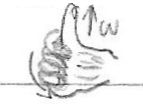
\includegraphics[scale=1.6]{rightHand}
	\caption{\textgreek{Μέθοδος του δεξιού χεριού (στη Φυσική)}}
	\label{fig:rightHand}
	\end{figure}
	
	\textbullet \quad $\displaystyle U = \omega \cdot r$  :  \textgreek{Σχέση γραμμικής και γωνιακής ταχύτητας} \linebreak 
	\textbullet \quad $\displaystyle f= \frac{N}{\Delta t} $ (1Hz = 1 rep / sec): \textgreek{Συχνότητα ταλάντωσης,} $N$  :  \textgreek{αριθμός ταλαντώσεων σε χρονικό διάστημα} $\Delta t$. \linebreak 
	\textgreek{Για} $\displaystyle N=1$, $\Delta t = T$  :  \textgreek{περίοδος ταλάντωσης. Άρα} $\displaystyle f=\frac{1}{T}$ \linebreak 
	\textbullet \quad $\displaystyle \omega = 2\pi f$ \linebreak 
	\textbullet \quad $\displaystyle a_c = \frac{U^2}{r} \ (\frac{m}{s^2}) $  :  \textgreek{κεντρομόλος επιτάχυνση} (centripetal acceleration). \textgreek{Έχει κατεύθυνση προς το κέντρο της κυκλικής τροχιάς}. \linebreak 
	\textbullet \quad $\displaystyle F_c = \frac{mU^2}{r} \ (N)$  :  \textgreek{Κεντρομόλος δύναμη. Έχει κατεύθυνση προς το κέντρο της κυκλικής τροχιάς} \linebreak 
	\textbullet \quad $\displaystyle F = G \frac{m_1m_2}{r^2} \ (N) $  :  \textgreek{Νόμος της παγκόσμιας έλξης} \linebreak 
	$G = 6.67 \cdot 10^{-11} (N\cdot m^2 / kg^2 ) $  :  \textgreek{σταθερά της παγκόσμιας έλξης. Ισχύει μόνο για σωμάτια, ή ομογενή σφαιρικά σώματα} $r$  :  \textgreek{απόσταση μεταξύ των κέντρων τους} $F$  :  \textgreek{δύναμη βαρυτικής έλξης} \linebreak 
	\textbullet \quad $\displaystyle \vec{g} = \frac{\vec{F}}{m} = G \frac{M}{r^2} \ (\frac{N}{kg} ) $  :  \textgreek{Ένταση του βαρυτικού πεδίου} $\vec{g}$ \textgreek{ίδια κατεύθυνση με το βάρος} \linebreak 
	\textbullet \quad \textgreek{Η σχέση δεν ισχύει για} $<r$, \textgreek{δηλαδή όταν το ελκούμενο σώμα βρίσκεται εντός του σώματος που "δημιουργεί" το βαρυτικό πεδίο} \linebreak 
	\textbullet \quad $\displaystyle U = \sqrt{G \frac{M}{r}} (\frac{m}{s}) $  :  \textgreek{Ταχύτητα περιστροφής των δορυφόρων} \linebreak 
	
	\textbullet \quad \uline{\textgreek{Επίσημη διατύπωση του 2ου Νόμου του Νεύτωνα}}: \textgreek{Η συνισταμένη των δυνάμεων που ασκούνται σε ένα σώμα, ισούται με το ρυθμό μεταβολής της ορμής του σώματος}. \linebreak 
	$\displaystyle \Sigma \vec{F} = \left( \frac{\Delta\vec{P}}{\Delta t} \right) = \frac{\delta \vec{P}}{\delta t} = \frac{d}{dt} (m \vec{U}) $, \textgreek{δηλαδή}: $\vec{P} = m \vec{U} (kg \cdot m / s) $  :  \textgreek{Ορμή}(Momentum) \linebreak 
	\textbullet \quad $\displaystyle m = \frac{F}{a} \ (kg) $  :  \textgreek{Αδρανειακή μάζα} \linebreak 
	\textbullet \quad $\displaystyle m = \frac{W}{g} \ (kg) $  :  \textgreek{Βαρυτική μάζα} \linebreak 
	\textbullet \quad $\displaystyle \vec{F} = \frac{\vec{p}_{\text{\textgreek{τελ.}}} - \vec{p}_{\text{\textgreek{αρχ.}}} }{\Delta t} $ \linebreak 
	\textbullet \quad \uline{\textgreek{Αρχή Διατήρησης Ορμής (Α.Δ.Ο.)}}: $\displaystyle \vec{P}_{\text{\textgreek{ΟΛ}}}^{\text{\textgreek{ΑΡΧ}}} = \vec{P}_{\text{\textgreek{ΟΛ}}}^{\text{\textgreek{ΤΕΛ}}} $ \linebreak 
	\textgreek{Η συνολική ορμή ενός μεμονωμένου συστήματος σωμάτων διατηρείται σταθερή}. \linebreak 
	
	\uline{\textgreek{Νόμοι Αερίων}} 
	\begin{enumerate} 
	\item \uline{\textgreek{Νόμος του} Boyle}: $\displaystyle p\cdot V = k = \text{\textgreek{σταθ.}}$ \textgreek{(ισόθερμη), όταν ο αριθμός των} $mol$ $n$ \textgreek{και η θερμοκρασία} $T$ \textgreek{είναι σταθερά}. 
	\item \uline{\textgreek{Νόμος} Charles}: $\displaystyle V \varpropto T$, \textgreek{όταν} $n, p$ \textgreek{σταθερά. \quad (ισοβαρής)} 
	\item \uline{\textgreek{Νόμος} Gay-Lussac}: $\displaystyle p \varpropto T$, \textgreek{όταν} $n, p$ \textgreek{σταθερά. Καταλήγουμε ότι}: (1, 2, 3 $\rightarrow$): $p \cdot V = n \cdot R \cdot T$  :  \uline{\textgreek{Καταστατική εξίσωση των ιδανικών αερίων}}.\textgreek{ Η εξίσωση ισχύει και για αέρια μείγματα. Ιδανικό αέριο είναι αυτό για το οποίο ισχύει η καταστατική εξίσωση ακριβώς, σε όλες τις πιέχεις και θερμοκρασίες}
	\end{enumerate}
	\textbullet \quad \textgreek{Επίσης, αν μιλάμε για συγκεκριμένο αέριο, μπορούμε από} (1) \textgreek{να πούμε ότι}: $\displaystyle p_1 \cdot V_1 = p_2 \cdot V_2$ \linebreak 
	\textbullet \quad $\displaystyle U_{\text{\textgreek{ΕΣ}}} = N \cdot \overset{-}{K}$  :  \textgreek{Εσωτερική ενέργεια αερίου (ουσιαστικά θερμική ενέργεια)} \linebreak 
	$\displaystyle \overset{-}{K} = \frac{(k_1 + k_2 + \ldots + k_n)}{N} $  :  \textgreek{μέση κινητική ενέργεια μορίων} \linebreak 
	\textbullet \quad $\displaystyle Q = \Delta U$  :  \textgreek{Προσφερόμενη θερμότητα = Αύξηση εσωτερικής ενέγειας αερίου} \linebreak 
	\textbullet \quad $\displaystyle W= P \cdot \Delta V$  :  \textgreek{Έργο που δημιουργεί η διαστολή αερίου}, $\Delta V$  :  \textgreek{αύξηση του όγκου αερίου κατά τη θέρμανση του} \linebreak 
	\textbullet \quad \textgreek{Από τα δύο προηγούμενα, αναγόμαστε στο εξής:} $\displaystyle Q = \Delta U + W$  :  \textgreek{Προσφερόμενη θερμότητα = Αύξηση Εσωτερικής Ενέργειας αερίου} $+$ \textgreek{Ενέργεια απαιτούμενη για την ανύψηση του εμβόλου. Η προηγούμενη σχέση ουσιαστικά αποτελεί την Α.Δ.Ε. για τα αέρια}. \linebreak 
	\textbullet \quad \textgreek{Θερμική ενέργεια = Τροφοδοτούμενη εν. - Αποδιδόμενη εν.} \linebreak 
	\textbullet \quad $\displaystyle U = \lambda \cdot f$  :  \textgreek{Θεμελιώδης Νόμος της Κυματικής} \linebreak 
	\textbullet \quad $\displaystyle \frac{1}{p} + \frac{1}{p'} = \frac{1}{f}$ , $f$  :  \textgreek{απόσταση εστίας - κορυφής, εστιακή απόσταση, ή απόσταση που συγκλίνουν οι ανακλώμενες ακτίνες και σχηματίζεται το είδωλο} (\figref{selofan}) \linebreak 
	$p'$  :  \textgreek{απόσταση ειδώλου μήκους} $P'Q'$ \textgreek{από την κορυφή}. \linebreak 
	
	\begin{figure}[H]
	\centering
	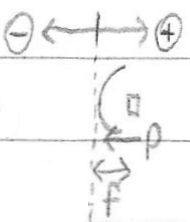
\includegraphics[scale=2]{selofan}
	\caption{\textgreek{Αναπαράσταση του θεμελιώδης νόμου της κυματικής}}
	\label{fig:selofan}
	\end{figure}
		
	\textbullet \quad \textgreek{Για σφαιρικό καθρέπτη ισχύει} $R = 2f$ (\textgreek{ακτίνα καμπυλότητας}) \linebreak 
	\textbullet \quad $\displaystyle m = -\frac{p'}{p} = \frac{\overset{---}{P'Q'}}{\overset{---}{PQ}} $ (\textgreek{μεγέθυνση}). \textgreek{Αν το είδωλο είναι ορθό η μεγέθυνση είναι \textgreek{θετική}, ενώ αν είναι αντεστραμμένο, η μεγέθυνση είναι αρνητική.} \linebreak 
	\textbullet \quad $\displaystyle n = \frac{C_0}{U}$  :  \textgreek{δείκτης διάθλασης, ή } $\displaystyle n =\frac{\sin (\theta_{\pi})}{\sin (\theta_{\delta})} $ \linebreak 
	$U$  :  \textgreek{ταχύτητα φωτός στο υλικό μέσο} \linebreak 
	\textgreek{Επίσης}: $\displaystyle n=\frac{\lambda_0}{\lambda} \leftrightarrow \lambda = \frac{\lambda_0}{n}$, $\lambda, n $  :  \textgreek{χαρακτηριστικό υλικού}. \linebreak 
	
	\textbullet \quad $\displaystyle \frac{\sin (\theta_{\pi})}{\sin (\theta_{\delta})} = \frac{n_2}{n_1} = \frac{U_1}{U_2}$ \uline{\textgreek{Νόμος του} Snell} (\figref{snell}) \linebreak 
	$\displaystyle \frac{\sin (\theta_{\pi})}{\sin (\theta_{\delta})} = $ \textgreek{σταθερό} \linebreak 
	
	\begin{figure}[H]
	\centering
	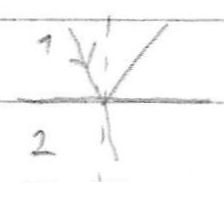
\includegraphics[scale=2]{snell}
	\caption{\textgreek{Ο Νόμος του} Snell \textgreek{ή Νόμος της διάθλασης}}
	\label{fig:snell}
	\end{figure}

	\textbullet \quad \uline{\textgreek{Νόμος της Ανάκλασης}} ( \textgreek{του Νεύτωνα}): \linebreak 
	\textgreek{Γωνία πρόσπτωσης} $\displaystyle (\theta_{\pi})$ = \textgreek{Γωνία ανάκλασης} $(\theta_a)$ \linebreak 
	\textbullet \quad $\displaystyle \sin (\theta_{\pi} = \frac{1}{n_{\text{\textgreek{ολ}}}} \rightarrow \theta_{\pi} $ \textgreek{οριακή γωνία} \linebreak 
	
	\textbullet \quad \uline{\textgreek{Νόμος} Brewster}: $\displaystyle \tan (\theta_{\pi}) = \frac{n_2}{n_1} \rightarrow \theta_{\pi} = $\textgreek{γωνία} Brewster, \textgreek{ή γωνία ολικής πόλωσης. Συμβαίνει όταν η ανακλώμενη και διαθλώμενη γωνία είναι κάθετες μεταξύ τους}. \linebreak 
	
	\subsection{Electrostatic Field} 
	
	\textbullet \quad $\displaystyle \vec{E} = \frac{\vec{F}}{q} = k \frac{|Q|}{r^2} \ \left( \frac{N}{C} \text{\textgreek{ή}} \frac{V}{m} \right) $ \textgreek{Ένταση (σε σημείο) ηλεκτροστατικού πεδίου, που δέχεται φορτίο} $q$ \textgreek{από φορτίο - πηγή} $Q$. \linebreak 
	\textbullet \quad $\displaystyle U_{\Sigma} = k \frac{Qq}{r} \ (J)$  :  \textgreek{Ηλεκτρική Δυναμική Ενέργεια} (electric potential energy); 
	\begin{small}
	\textgreek{η οποία ανήκει και στα δύο φορτία -ανήκει στο σύστημα-} 
	\end{small} \textgreek{κινούμενου φορτίου} $q$ \textgreek{σε σημείο} $\Sigma$ \textgreek{του πεδίου}, $r$  :  \textgreek{απόσταση μεταξύ} $q$ \textgreek{και} $Q$. \linebreak 
	\textbullet \quad $\displaystyle V_{\Sigma} = \frac{U_{\Sigma}}{q} = k \frac{Q}{r} \ (V) $  :  \textgreek{Δυναμικό ηλεκτροστατικού πεδίου} ( Coulomb), \textgreek{σε θέση Χ του πεδίου}, $r$  :  \textgreek{απόσταση μεταξύ του σημείου Σ και του φορτίου} $Q$ \textgreek{που δημιουργεί το πεδίο. Αντίστοιχα ισχύει ότι:} $\displaystyle V_{\text{\textgreek{ΣΡ}}} = \frac{W_{\Sigma \to P}}{q} \ (V) = V_{\Sigma} - V_P$  :  \textgreek{Διαφορά Δυναμικού, ή τάση μεταξύ δύο σημείων Σ και Ρ του ηλεκτρικού πεδίου} \linebreak 
	\textbullet \quad $\displaystyle C = \frac{Q}{V} \ (F) \ (Farad = \frac{Coulomb}{Volt}$  :  \textgreek{Χωρητικότητα του πυκνωτή}, $Q$ = \textgreek{φορτίο πυκνωτή}, $V$ = \textgreek{διαφορά δυναμικού μεταξύ των οπλισμών του πυκνωτή. Μασ πληροφορεί για το φορτίο που μπορεί να αποθηκευτεί ανά μονάδα τάσης μεταξύ των οπλισμών του}. \linebreak 
	\textbullet \quad $\displaystyle C = \epsilon \cdot \epsilon_0 \frac{S}{l} \ (F) $  :  \textgreek{Εξάρτηση χωρητικότητας \uline{επίπεδου} πυκνωτή από σχετική διηεκτρική σταθερά } $\epsilon$ \textgreek{του διηλεκτρικού που βρίσκεται μεταξύ των οπλισμών του}, $S$  :  \textgreek{εμβαδό πλάκας πυκνωτή}, $l$  :  \textgreek{απόσταση μεταξύ των πλακών του} \linebreak 
	$\displaystyle U = \frac{1}{2} CV^2 = \frac{1}{2} Q \cdot V = \frac{1}{2} \frac{Q^2}{C} (J) $  :  \textgreek{Ηλεκτρική δυναμική ενέργεια του πυκνωτή} \linebreak 
	\textbullet \quad $\displaystyle E = \frac{V}{l} \ \frac{V}{m} $  :  \textgreek{Ένταση ομογενούς ηλεκτροστατικού πεδίου, άρα μόνο για επίπεδο πυκνωτή} \linebreak 
	\textbullet \quad \uline{\textgreek{Αρχή Διατήρησης του Φορτίου}}: \textgreek{Όσο φορτίο διέρχεται από κάποια διατομή του αγωγού στη μονάδα του χρόνου} \linebreak 
	\textbullet \quad $\displaystyle \Sigma I_{\text{\textgreek{εισ.}}} = \Sigma I_{\text{\textgreek{εξ.}}}$  :  \uline{\textgreek{1ος κανόνας Kirchoff}}: \textgreek{Το άθροισμα των εντάσεων των ρευμάτων, που "εισέρχονται" σ'έναν κόμβο, ισούται με το αθροισμα των εντάσεων των ρευμάτων, που "εξέρχονται" από αυτόν, ή} $\Sigma I = 0 $ \textgreek{στο κόμβο αυτό} \linebreak 
	\textbullet \quad $\displaystyle \Sigma (\Delta V) = 0 $  :  \uline{\textgreek{2ος κανόνας} Kirchoff}: \textgreek{Κατά μήκος μιας κλειστής διαδρομής σε ένα κύκλωμα, το αλγεβρικό άθροισμα των διαφορών δυναμικού  είναι}$0$. \linebreak 
	\textbullet \quad $\displaystyle V_{\text{\textgreek{ΠΗΓ}}} = \epsilon - I r_{\text{\textgreek{εσ}}} \ (V) $  :  \textgreek{Πολική τάση πηγής, ή τάση στους πόλους της πηγής}, $I$ = \textgreek{ρεύμα κυκλώματος}, $\displaystyle r_{\text{\textgreek{εσ}}}$  :  \textgreek{Εσωτερική αντίσταση πηγής}, $\displaystyle V_{\text{\textgreek{ΠΗΓ}}}$  :  \textgreek{τάση στους πόλους της πηγής}. \linebreak 

	\textbullet \quad $E=h \cdot f \ (j)$  :  \textgreek{Ενέργεια φωτονίου} \linebreak 
	\textbullet \quad $L = mUr$  :  \textgreek{Μέτρο στροφορμής του ηλεκτρονίου} \linebreak 
	\textbullet \quad $\displaystyle \hbar = \frac{h}{2\pi}$  :  \textgreek{Μειωμένη σταθερά} Planck. \textgreek{Από τα προηγούμενα συμπεραίνουμε ότι η στροφορμή του ηλεκτρονίου μπορεί να πάρει τιμές ίσες με τα ακέραια πολλαπλάσια της ποσότητας} $\hbar$. \textgreek{Ηλεκτρόνια με την ίδια στροφορμή κινούνται σε μία από τις επιτρεπόμενες τροχιές, ακτίνας} $r$, \textgreek{δλδ.}: $\displaystyle mUr = n \hbar \ , n \in \mathbb{N}$. \textgreek{Υποδηλώνεται έτσι η κβάντωση της στροφορμής}. \linebreak 
	\textbullet \quad $\displaystyle E_{\text{\textgreek{αρχ}}}-E_{\text{\textgreek{τελ}}} = h \cdot f \ (J)$  :  \textgreek{Ενέργεια που παράγεται όταν ηλεκτρόνιο μεταπηδά από μία επιτρεπόμενη τροχιά σε άλλη μικρότερης ενέργειας}. \linebreak 
	\textbullet \quad $\displaystyle E_{\text{\textgreek{ΟΛ}}} = E_K + U+{\Delta} = k\frac{e^2}{2r} + \left( -k \frac{e^2}{4} \right) = -\frac{ke^2}{2r}$  :  \textgreek{Ολική ενέργεια ηλεκτρονίου του ατόμου του υδρογόνου (στο σύστημα ηλεκτρονίου ηλεκτρονίου - πυρήνα)}. \linebreak 
	\textbullet \quad $r_n = n^2 \cdot r_1 \ (m)$  :  \textgreek{Ακτίνα επιτρεπόμενων τροχιών}. \linebreak 
	$\displaystyle n\in \mathbb{N}^*$  :  \textgreek{κύριος κβαντικός αριθμός}. $\displaystyle r_1 = \frac{\hbar^2}{mkq_e^2} = 0.53 \cdot 10^{-10} m =$ \textgreek{ακτίνα} Bohr \linebreak 
	\textbullet \quad $1$ev = $1.6 \cdot 10^{-19} \ (J)$  :  \textgreek{Το ηλεκτρονιοβόλτ είναι η ενέργεια που μεταβιβάζεται σε ένα ηλεκτρόνιο όταν αυτό επιταχύνεται μέσω διαφοράς δυναμικού} 1V. \linebreak 
	\textbullet \quad $\displaystyle E_n = \frac{E_1}{n^2} \ (J)$  :  \textgreek{Επιτρεπόμενες τιμές ενέργειας}, $E_1 = - \frac{mk^2e^4}{2\hbar^2} = - 13.6 $eV \linebreak 
	\textbullet \quad $\displaystyle E_{\text{\textgreek{ιονισμού}}} = E_{\infty} - E_1$  :  \textgreek{Ποσότητα ενέργειας που απαιτείται για την απομάκρυνση του ηλεκτρονίου εκτός του ηλεκτρικού πεδίου του πυρήνα}. \linebreak 
	\textbullet \quad $\displaystyle \lambda_{MIN} = \frac{ch}{eV} \ (m)$  :  \textgreek{Μικρότερο μήκος κύματος της ακτινοβολίας που εκπέμπεται, όταν η ενέργεια του ηλεκτρονίου μετατρέπεται σε ενέργεια φωτονίου σε μία μόνο κρούση}($\displaystyle k_{\text{\textgreek{τελ}}} = 0$), $V$  :  \textgreek{τάση που επιταχύνει τη δέσμη ηλεκτρονίων} \linebreak 
	
	\textbullet \quad \textgreek{Η} \uline{\textgreek{ατομική μονάδα μάζας}} (atomic mass unit = amu) \textgreek{ορίζεται ως το 1/12ο της μάζας του ατόμου του άνθρακα-12} $ ^{12}C, $ 1amu = $1.66\cdot 10^{-24}$g. \linebreak 
	\textbullet \quad \uline{\textgreek{Σχετική ατομική μάζα}}, \textgreek{ή} \uline{\textgreek{ατομικό βάρος}} $A_r$ \textgreek{λέγεται ο αριθμός που δείχνει πόσες φορές είναι μεγαλύτερη η μάζα του ατόμου του στοιχείου από το} 1amu. \linebreak 
	$\displaystyle A_r = \frac{m_{\text{\textgreek{ατόμου}}}}{1.66\cdot 10^{-27} \text{kg}} $ \linebreak 
	\textbullet \quad \textgreek{Το} mol \textgreek{είναι μονάδα ποσότητας ουσίας στο} $S.I.$ \textgreek{και ορίζεται ως η ποσότητα της ύλης που περιέχει τόσες στοιχειώδεις οντότητες, όσος είναι ο αριθμός των ατόμων που υπάρχουν σε} $12$g \textgreek{του άνθρακα -12} $^{12}C$. \textgreek{Ο αριθμός των ατόμων που υπάρχουν σε 12}g \textgreek{του} $^{12}C$ \textgreek{ονομάζεται αριθμός} Avogadro ($N_A$) \textgreek{και υπολογίστηκε πειραματικά πως είναι ίσος με}: $\displaystyle N_A \simeq 6.0252 \cdot 10^{-23}$ mol$^{-1}$. \textgreek{Με άλλα λόγια} $1$ mol \textgreek{είναι η ποσότητα μιας ουσίας που περιέχει} $N_A$ \textgreek{οντότητες}. \linebreak 
	\textbullet \quad \textgreek{Ο αριθμός} Avogadro \textgreek{εκφράζει τον αριθμό των ατόμων οποιουδήποτε στοιχείου που περιέχονεται σε μάζα τόσων γραμμαρίων όσο είναι η σχετική ατομική μάζα του. Μπορούμε να πούμε ότι} 1mol \textgreek{ατόμων περιέχει} $N_A$ \textgreek{άτομα και ζυγίζει} $A_r$g. \linebreak 
	(1g $\simeq 1.66 \cdot 10^{-23} \ A_r$) \linebreak 
	\textbullet \quad \textgreek{Ο αριθμός} Avogadro \textgreek{εκφράζει τον αριθμό των μορίων στοιχείου χημικής ένωσης που περιέχονται σε μάζα τόσων γραμμαρίων όσο είναι η σχετική ατομική μάζα τους. Δηλαδή,} \linebreak 
	1mol \textgreek{μορίων περιέχει} $N_A$\textgreek{μόρια και ζυγίζει} $M_r$ g. \linebreak 
	\textbullet \quad \uline{\textgreek{Γραμμομοριακή μάζα}} M \textgreek{ενός στοιχείου ή μίας χημικής ένωσης είναι η μάζα ενός} mole \textgreek{μορίων της και μετριέται στο} S.I. \textgreek{σε} kg / mol. \textgreek{Η γραμμομοριακή μάζα} (molar mass) \textgreek{είναι} 1,000 \textgreek{φορές μικρότερη από τη σχετική μοριακή μάζα (μοριακή βάρος)} $M_r$  :  $\displaystyle \therefore M = \frac{M_r}{1000}$ \linebreak 
	\textbullet \quad \uline{\textgreek{Γραμμομοριακός, ή μοριακός όγκος αερίου}} ($V_m$) \textgreek{ονομάζεται ο όγκος που καταλαμβάνει} 1mol \textgreek{αυτού, σε ορισμένες συνθήκες πίεσης και θερμοκρασίας. Σε πρότυπες συνθήκες πίεσης} (1atm) \textgreek{και θερμοκρασίας} ($0^{\circ} C$) - S.T.P., \textgreek{ο γραμμομοριακός όγκος των αερίων βρέθηκε πειραματικά ότι είναι ίσος με} 22.4L, \textgreek{δλδ.:} $\displaystyle V_m = 22.4 \frac{L}{\text{mol}} $ \textgreek{σε} STP \textgreek{συνθήκες. (δλδ.} $V \varpropto n$). \linebreak 
	\textbullet \quad $N_A$ \textgreek{άτομα} $\leftrightarrow 1$ mol \textgreek{ατόμων} $\leftrightarrow A_r g$ \textgreek{μέσω του μοριακού τύπου} \linebreak 
	\textbullet \quad $N_A$ \textgreek{μόρια} $\leftrightarrow 1$ mol \textgreek{μορίων} $\leftrightarrow M_r g$ \quad STP \textgreek{και μόνο για αέρια} \linebreak 
	\textbullet \quad $N_A$ \textgreek{οντότητες αέριας ουσίας} $ \leftrightarrow 1$ mol \textgreek{αέριας ουσίας} $\leftrightarrow V_m = 22.4$L \linebreak 
	\textbullet \quad \textgreek{Αριθμός των} mol \textgreek{ουσίας}: $\displaystyle n = \frac{m_{\text{\textgreek{ΟΛ}}}}{M}$, $m_{\text{\textgreek{ΟΛ}}}$  :  \textgreek{ολική μάζα ουσίας} \linebreak 
	\textbullet \quad \textgreek{Η μεταβολή στην οποία η θερμοκρασία παραμένει σταθερή ονομάζεται \uline{ισόθερμη}}. \linebreak 
	\textbullet \quad \textgreek{Η μεταβολή στην οποία ο όγκος παραμένει σταθερός ονομάζεται \uline{ισόχωρη}}. \linebreak 
	\textbullet \quad \textgreek{Η μεταβολή στην οποία η πίεσης παραμένει σταθερή ονομάζεται \uline{ισοβαρής}}. \linebreak 
	\textbullet \quad $\displaystyle p=\frac{1}{3} \frac{Nm\overset{-}{U}^2}{V} $  :  \textgreek{Σχέση πίεσης με τη μέση τιμή των ταχυτήτων των μορίων του αερίου}, $m$  :  \textgreek{μάζα κάθε μορίου}, $N$  :  \textgreek{πλήθος μορίων}, $V$  :  \textgreek{όγκος δοχείου}. \linebreak 
	\textbullet \quad $\displaystyle \overset{~}{U} = \sqrt{\overset{-}{U}^2} = \sqrt{\frac{3kT}{m}}$  :  \textgreek{Σχέση ταχύτητας} ($U$) \textgreek{με τη θερμοκρασία} $(T)$ \textgreek{(των μορίων) του αερίου,} \linebreak 
	$M$  :  \textgreek{η γραμμομοριακή μάζα}, $U_{\pi}$  :  \textgreek{πιθανότερη τιμή} \linebreak 
	\textbullet \quad $\displaystyle \frac{1}{2} m \overset{-}{U}^2 = \frac{3}{2}kT$  :  \textgreek{Η μέση Κ.Ε. των μορίων του ιδανικού αερίου είναι ανάλογη με την απόλυτη θερμοκρασία}. \linebreak 
	\textbullet \quad \textgreek{Οι ταχύτητες των μορίων κάποιας ποσότητας αερίου σε θερμοκρασία} $T$ \textgreek{ακολουθούν την κατανομή} Maxwell-Boltzmann. \linebreak 
	\textbullet \quad \textgreek{Έπειτα από} n \textgreek{χρόνους υποδιπλασιασμού (ημιζωές)} ($t_{1/2}$) \textgreek{ραδιενεργού ισοτόπου έχει απομείνει}: $\displaystyle m= (\frac{1}{2})^n \cdot m_0$ \linebreak 
	$m_0$  :  \textgreek{ποσότητα αρχικής, ραδιενεργούς ουσίας} \linebreak 
	
	\text{\textgreek{Μονάδες Ραδιενέργειας}}: 
	\begin{enumerate}
	\item \textgreek{Μονάδες που εκφράζουν το επίπεδο ραδιενέργειας ενός υλικού}. \linebreak 
	\textgreek{Συνηθέστερη μονάδα είναι το} Curie(Ci), \textgreek{που είναι ποσότητα ουσίας που υφίσταται} $3.7 \cdot 10^{10}$ \textgreek{ραδιενεργές διασπάσεις ανά δευτερόλεπτο}. \linebreak 
	\textgreek{Στο} S.I. \textgreek{μονάδα ραδιενέργειας είναι το} Becquerel (Bq), \textgreek{που αντιστοιχεί σε μία ραδιενεργό διάσπαση ανά δευτερόλεπτο, δλδ.} $1Ci = 37\cdot 10^9 Bq$. \linebreak 
	\textgreek{Μονάδες που εκφράζουν την απορροφούμενη ακτινοβολία από έναν οργανισμό}. \linebreak 
	\textgreek{Για ποσοτική εκτίμηση των αποτελεσμάτων της επίδρασης της ακτινοβολίας, θεσπίστηκες το} RAD (Radiation Absorbed Dose) \textgreek{που εκφράζει δόση ακτινοβολίας, η οποία απελευθερώνει} $10^{-2}$J \textgreek{ενέργειας ανά} kg \textgreek{βάρους του σώματος που την απορροφά. Στο} SI \textgreek{μονάδα είναι το} Gray(Gy) \linebreak 
	1Gy = 100 RAD 
	\item \textgreek{Μονάδες που εκφράζουν την απορροφούμενη ακτινοβολία από έναν οργανισμό σε σχέση με τις βιολογικές επιπτώσεις που προκαλούν}. \linebreak 
	\textgreek{Το} REM (Radiation Equivalent Man) \textgreek{είναι μια μονάδα ραδιενέργειας που δεν εξαρτάται από το είδος της ακτινοβολίας και εκφράζει τις βιολογικές καταστροφές που προκαλούνται στον άνθρωπο από την απορρόφηση των διαφόρων ακτινοβολιών. Δηλαδή} 1rem \textgreek{είναι ποσότητα ακτινοβολίας, η οποία επιφέρει ένα συγκεκριμένο βιολογικό αποτέλεσμα.} \linebreak 
	1rem = 1rad \textgreek{ακτινών Χ ή γ. 1}Gy \textgreek{ακτινοβολίας α προκαλεί 20 φορές μεγαλύτερη καταστροφή στους ανθρώπινους ιστούς από 1} Gy \textgreek{ακτινοβολίας γ}.
	\end{enumerate}
	
	\subsection{Thermodynamics} 
	
	\textbullet \quad \textgreek{Όταν σ'ένα θερμοδυναμικό σύστημα οι θερμοδυναμικές μεταβλητές, δηλαδή η πίεση}($p$), \textgreek{η πυκνότητα}($p$) \textgreek{και η θερμοκρασία} ($T$), \textgreek{που το περιγράφουν διατηρούνται σταθερές με το χρόνο, τότε το σύστημα βρίσκεται σε κατάσταση θερμοδυναμικής ισορροπίας. Η κατάσταση θερμοδ. ισορ. ενός συστήματος μπορεί να παρασταθεί γραφικά με ένα σημείο. Ένα σύστημα που δεν βρίσκεται σε ισορροπία δεν παριστάνεται γραφικά}. \linebreak 
	\textbullet \quad $\displaystyle \Delta W = p \Delta V$  :  \textgreek{στοιχειώδες έργο} $(\Delta W)$ \textgreek{της δύναμης που ασκεί το αέριο (πίεσης} $p$) \textgreek{στο σώμα (π.χ. έμβολο) μετατοπίζοντας το, κατά όγκο} $\Delta V$. \linebreak 
	\textbullet \quad $U = \frac{3}{2} nRT \ (J)$  :  \textgreek{Η εσωτερική ενέργεια ορισμένης ποσότητας ιδανικού αερίου εξαρτάται μόνο από τη θερμοκρασία του}. \linebreak 
	\textbullet \quad \uline{\textgreek{1ος θερμοδυναμικός νόμος}}: $\displaystyle Q = \Delta U + W$ \linebreak 
	\textgreek{Το ποσό θερμότητας} ($Q$) \textgreek{που απορροφά ή αποβάλλει ένα θερμοδυναμικό σύστημα είναι ίσο με το αλγεβρικό άθροισμα της μεταβολής της εσωτερικής του ενέργειας και του έργου που παράγει ή δαπανά το σύστημα}. \linebreak 
	\textbullet \quad \textgreek{Ειδική γραμμομοριακή θερμότητα αερίου υπό σταθερή πίεση} (constant pressure specific heat): $C_p$ \linebreak 
	\textgreek{Ισχύει:} $\displaystyle Q_p = n C_p \Delta T$  :  
	\begin{small}
	\textgreek{θερμότητα που απορροφά το αέριο όταν θερμαίνεται υπό σταθερό όγκο}
	\end{small} \linebreak 
	\textbullet \quad \textgreek{Ειδική γραμμομοριακή θερμότητα αερίου υπό σταθερό όγκο:} $C_v$ \linebreak 
	\textgreek{Θα ισχύει}: $\displaystyle Q_v = n C_v \Delta T$  :  \begin{small}
	\textgreek{θερμότητα που απορροφά το αέριο όταν θερμαίνεται υπό σταθερό όγκο}
	\end{small} \linebreak 
	\textbullet \quad \textgreek{Από τον 1ο Ν.Δ. προκύπτει ότι:} $\displaystyle C_p - C_v + R$ \linebreak 
	\textbullet \quad $\displaystyle \gamma = \frac{C_p}{C_v} \ , \ \gamma > 1$ \linebreak 
	
	\textgreek{Εφαρμογή του 1ου θερμοδυναμικού νόμου} \linebreak 
	\textbullet \quad A) \textgreek{Ισόθερμη Αντιστρεπτή μεταβολή} \linebreak 
	\textgreek{Έργο: } $\displaystyle W = nRT \ln \left( \frac{V_{\text{\textgreek{τελ}}}}{V_{\text{\textgreek{αρχ}}}} \right)$, \textgreek{αφού} $T = $ \textgreek{σταθ.} $\rightarrow Q = W$ \linebreak 
	\textbullet \quad \textgreek{Στην ισόθερμη εκτόνωση όλο το ποσό θερμότητας που απορροφά το αέριο μετατρέπεται σε μηχανικό έργο}. \linebreak 
	\textbullet \quad B) \textgreek{Ισόχωρη Αντιστρεπτή μεταβολή} \linebreak 
	$Q= \Delta U$  :  \textgreek{Στην ισόχωρη θέρμανση όλο το ποσό θερμότητας που απορρόφησε το αέριο χρησιμοποιήθηκε για την αύξηση της εσωτερικής του ενέργειας}. \linebreak 
	\textbullet \quad \textgreek{Γ) Ισοβαρής Αντιστρεπτή μεταβολή} \linebreak 
	\textgreek{Έργο}: $\displaystyle W = p \left( V_{\text{\textgreek{τελ}}} - V_{\text{\textgreek{αρχ}}} \right)$, \textgreek{Από τον 1ο Θ.Ν.:} $\displaystyle Q = \Delta U + p \left(V_{\tau} - V_{\alpha} \right)$. \linebreak 
	\textgreek{Στην ισοβαρή θέρμανση ένα μέρος από το ποσό θερμότητας που απορρόφησε το αέριο από το περιβάλλον χρησιμοποήθηκε για την αύξηση της εσβτερικής του ενέργειας και το υπόλοιπο αποδόθηκε εκ νέου στο περιβάλλον υπό μορφή έργου}. \linebreak 
	\textbullet \quad \textgreek{Δ) Αδιαβατική Μεταβολή} \linebreak 
	\textgreek{Μεταβολή κατά την οποία δε συντελείται μεταφορά θερμότητας από το περιβάλλον στο σύστημα και αντίστροφα.} \linebreak 
	$\displaystyle pV^{\gamma} =$ \textgreek{σταθ.: Νόμος του} Poisson \textgreek{που διέπει τη μεταβολή}. \linebreak 
	\textgreek{Από τον 1ο Θ.Ν.: } $\displaystyle 0 = \Delta U + W \leftrightarrow W = -\Delta U$ \linebreak 
	\textbullet \quad \textgreek{Ε) Κυκλική Αντιστρεπτή μεταβολή} \linebreak 
	\textgreek{Κυκλική ονομάζουμε τη μεταβολή στην οποία το σύστημα μετά από μια διεργασία επιστρέφει στην ίδια κατάσταση} $\therefore Q = W$ \linebreak 
	
	\textgreek{Υπολογισμός μεγεθών κίνησης απ'τα Διαγράμματα} \linebreak 
	\textbullet \quad \textgreek{Διάγραμμα επιτάχυνσης - χρόνου: το εμβαδόν από το γράφημα μέχρι τον άξονα του χρόνου μας δίνει τη μεταβολή της ταχύτητας}. \linebreak 
	\textbullet \quad \textgreek{Διάγραμμα ταχύτητας - χρόνου: το εμβαδόν από το γράφημα μέχρι τον άξονα του χρόνου μας δίνει τη μετατόπιση}$\Delta x$  :  \textgreek{η κλίση της ευθείας μας δίνει την επιτάχυνση} \linebreak 
	\textbullet \quad \textgreek{Διάγραμμα θέσης - χρόνου: η κλίση της ευθείας μας δίνει την ταχύτητα του σώματος} \linebreak 
	
	\uline{\textgreek{Ταλαντώσεις}} \linebreak 
	\textbullet \quad \textgreek{Το έργο δύναμη} $F$ \textgreek{βρίσκεται από το εμβαδόν της} $F = f(x)$ \textgreek{μέχρι τον οριζόντιο άξονα} $x$. \linebreak 
	\textbullet \quad \textgreek{Ιδιοσυχνότητα ελεύθερης ταλάντωσης}: $\displaystyle f_0 = \frac{1}{2\pi} \sqrt{\frac{k}{m}}$ , \linebreak 
	$m$  :  \textgreek{σώμα που ταλαντώνεται}, $k$  :  \textgreek{σταθερά ελατηρίου. Μιλάμε ιδανικά. Στην πραγματικότητα η} $f_0$ \textgreek{θα είναι λίγο μικρότερη αφού απαιτείται επιπλέον δύναμη για να διατηρηθεί ως έχει}. \linebreak 
	
	\textbullet \quad $\displaystyle T = F \cdot l \ (N\cdot m)$  :  \textgreek{Ροπή δύναμης} $F, l$  :  \textgreek{(κάθετη) απόσταση μεταξύ άξονα περιστροφής και σημείου εφαρμογής της δύναμης. Η ροπή έχει τη διεύθυνση του άξονα περιστροφής και η φορά της δίνεται από τον κανόνα του δεξιού χεριού}. \linebreak 
	\textbullet \quad $W = T \cdot \theta$ (J): \textgreek{Έργο κατά τη στροφική κίνηση που προκαλείται από στροφική δύναμη (ροπή). Για να το υπολογίσουμε χωρίζουμε τη γωνία} $\theta$ \textgreek{σε απειροστά μικρές γωνίες} $d\theta_1, d\theta_2, \ldots$ \textgreek{και αθροίζουμε τα αντίστοιχα έργα. Αν η ροπή της δύναμης παραμένει σταθερή το έργο δίνεται από τον παραπάνω τύπο.} \linebreak 
	\textbullet \quad \textgreek{Προώθηση του πυραύλου:} $\displaystyle U_{\text{\textgreek{τελ}}} - U_{\text{\textgreek{αρχ}}} = U_{\text{\textgreek{σχ. αερίων}}} \ln \left( \frac{M_{\text{\textgreek{αρχ}}}}{M_{\text{\textgreek{τελ}}}} \right) $ \linebreak 
	$\displaystyle U_{\text{\textgreek{σχ. αερίων}}}$ = \textgreek{σχετική ταχύτητα αερίων} \linebreak 
	\textgreek{Η προώθηση του στηρίζεται στην Α.Δ.Ο., επομένως με την εξίσωση αυτή, μελετάμε την προώθηση του στο διάστημα, μακριά από κάθε βαρυτική έλξη, όπου μπορούμε έτσι να θεωρήσουμε το σύστημα μονωμένο.}\linebreak 
	\textbullet \quad \uline{\textgreek{Φαινόμενο} Doppler}: \textgreek{πηγή} = $S$, \textgreek{παρατηρητής} = $A$  
	\begin{enumerate}
	\item \textgreek{Ακίνητη πηγή - Ακίνητος παρατηρητής}: $f_A = f_s = \frac{U}{\lambda} $, \linebreak 
	\textgreek{όπου}: $U, \lambda$ \textgreek{η ταχύτητα και το μήκος του κύματος που εκπέμπει η πηγή}
	\item \textgreek{Ακίνητη πηγή - Κινούμενος παρατηρητής με ταχύτητα} $U_A$ \linebreak
	$\displaystyle f_A = \frac{U \pm U_A}{U} f_s $, +: \textgreek{παρατηρητής απομακρύνεται από την πηγή και -: όταν πλησιάζει σε αυτή.} \linebreak 
	\item \textgreek{Κινούμενη πηγή με ταχύτητα} $U_s$ - \textgreek{Ακίνητος παρατηρητής:}
	$\displaystyle f_A = \frac{U}{U\pm U_s} f_s$, +: \textgreek{πηγή απομακρύνεται από τον παρατήρητη, ενώ -: πλησιάζει}
	\item \textgreek{Κινούμενη πηγή με ταχύτητα} $U_s$ - \textgreek{Κινούμενος παρατηρητής με ταχύτητα} $U_A$  : \linebreak 
	$\displaystyle f_A = \frac{U \pm U_A}{U \mp U_s} f_s$, \begin{small}
	$\displaystyle \frac{+}{-}$  :  \textgreek{όταν πλησιάζουν}, $\displaystyle \frac{-}{+}$  :  \textgreek{όταν απομακρύνονται} 
	\end{small} \linebreak 
	\end{enumerate} 
	
	\textbullet \quad $\displaystyle e = \frac{W}{Q_h}$  :  \textgreek{Συντελεστής απόδοσης οποιασδήποτε μηχανής} \linebreak 
	$Q_n$  :  \textgreek{θερμότητα με την οποία τροφοδοτούμε τη μηχανή} \linebreak 
	\textbullet \quad \textgreek{Στην κυκλική μεταβολή το έργο που παράγει το αέριο ισούται με το καθαρό ποσό θερμότητας που απορροφά, το οποίο είναι ίσο με το ποσό θερμότητας που τροφοδοτείται μείον το ποσό θερμότητας που αποβάλλει} $Q_c$. \linebreak 
	$\displaystyle e= 1 -\frac{|Q_c|}{Q_h}$ \linebreak 
	\textbullet \quad \uline{\textgreek{Μηχανή} Carnot}: $\displaystyle e_{\text{carnot}} = 1 - \frac{T_c}{T_h}$ \linebreak 
	$T_c$  :  \textgreek{θερμοκρασία ψυχρής δεξαμενής} \linebreak 
	$T_h$  :  \textgreek{θερμοκρασία θερμής δεξαμενής} \linebreak 
	\textgreek{Δεν μπορεί να υπάρξει θερμική μηχανή που να έχει μεγαλύτερη απόδοση από μια μηχανή} Carnot \textgreek{η οποία λειτουργεί ανάμεσα στις δύο θερμοκρασίες}. \linebreak 
	
	\textbullet \quad \uline{\textgreek{2ος θερμοδυναμικός νόμος}} \linebreak 
	\textbullet \quad \textgreek{Είναι αδύνατο να κατασκευαστεί μηχανή που να μετατρέπει εξ ολοκλήρου τη θερμότητα σε ωφέλιμο έργο.} \linebreak 
	\textbullet \quad \textgreek{Είναι αδύνατο να κατασκευαστεί μηχανή που να μεταφέρει θερμότητα από ένα ψυχρό σώμα σε ένα θερμότερο, χωρίς να δαπανάται ενέργεια για τη λειτουργία της}. \linebreak 
	\textbullet \quad $\displaystyle \Delta S = \int \frac{\Delta Q}{T} $ (J/k): \textgreek{Η μεταβολή της εντροπίας} ($\Delta S$) \textgreek{συστήματος κατά τη διάρκεια μιας πολύ μικρής αντιστρεπτής μεταβολής, τόσο μικρής ώστε η θερμοκρασία του συστήματος να μπορεί να θεωρηθεί σταθερή}. \linebreak 
	\textgreek{Όταν σε μια αντιστρεπτή μεταβολή το} $\Delta Q$ \textgreek{είναι θετικό όταν το σύστημα απορροφά θερμότητα, επομένως η εντροπία αυξάνεται. Ισχύει και το αντίθετο}. \linebreak 
	\textbullet \quad \textgreek{Από μακροσκοπική άποψη η αύξηση της εντροπίας οδηγεί σε μείωση της ικανότητας του συστήματος να παράγει ωφέλιμο έργο, ενώ από μικροσκοπική άποψη η αύξηση της εντροπίας οδηγεί σε αύξηση της αταξίας του συστήματος} \linebreak 
	
	\uline{\textgreek{Περίπτωσεις υπολογισμού μεταβολής της εντροπίας}} \linebreak 
	\textbullet \quad \textgreek{Αδιαβατική αντιστρεπτή μεταβολή:} $\Delta S = 0$ \linebreak 
	\textbullet \quad \textgreek{Ισόθερμη αντιστρεπτή μεταβολή:} $\displaystyle \Delta S = \frac{Q}{T}$ \linebreak 
	\textbullet \quad \textgreek{Κυκλική μεταβολή}: $\displaystyle \Delta S_{\text{\textgreek{ΟΛ}}} = 0$ \linebreak 
	\textbullet \quad \textgreek{Ελεύθερη εκτόνωση}: $\displaystyle \Delta S = nR\ \left( \frac{V_B}{V_A} \right) $ \linebreak 
	
	\textbullet \quad \textgreek{Το έργο στην αδιαβατική αντιστρεπτή μεταβολή είναι}: \linebreak 
	$\displaystyle W = \frac{p_{\text{\textgreek{τελ}}} V_{\text{\textgreek{τελ}}} - p_{\text{\textgreek{αρχ}}} V_{\text{\textgreek{αρχ}}}}{1-\gamma} $ \linebreak 
	\textbullet \quad \textgreek{Η μεταβολή στην εσωτερική ενέργεια ενός αερίου δίνεται από τη σχέση}: $\displaystyle \Delta U = nC_v \Delta T$ \linebreak 
	\textbullet \quad \textgreek{Θερμικές μηχανές ονομάζουμε αυτές που μετατρέπουν τη θερμότητα σε μηχανικό έργο}. \linebreak 
	
	\subsection{Electric Field}
	
	$\displaystyle \vec{\Phi}_E = \vec{E}\cdot A\cos (\theta) \ (N \cdot m^2 / C) $  :  \textgreek{Ηλεκτρική ροή που διέρχεται από μια επίπεδη επιφάνεια, εμβαδού Α, η οποία βρίσκεται μέσα σε ομογενές ηλεκτρικό πεδίο έντασης Ε}. \linebreak 
	$\theta$  :  \textgreek{η γωνία που σχηματίζει το κάθετο στην επιφάνεια διάνυσμα Α με τη διεύθυνση των δυναμικών γραμμών} \linebreak 
	\textbullet \quad \textgreek{Στη γενικότερη περίπτωση όπου η επιφάνεια δεν είναι επίπεδη και βρίσκεται μέσα σε ανομοιογενές ηλ. πεδίο}: \linebreak 
	$\displaystyle \vec{\Phi}_E = \sum \limits_{i=1}^n \vec{E}_i \Delta A_i \cos (\theta_i)$ , \textgreek{όπου} $n$ \textgreek{το πλήθος των τμήσεων της επιφάνειας Α σε στοιχειώδεις επιφάνειες επίπεδες και σταθερής έντασης}. \linebreak 
	\textbullet \quad $\displaystyle \Phi_E = \frac{Q_{\text{\textgreek{εγκ}}}}{\epsilon_0}$  :  \uline{\textgreek{Νόμος του Γκάους}} \textgreek{για το ηλ. πεδίο} \linebreak 
	\textgreek{Η ηλεκτρική ροή που διέρχεται από μια} \uline{\textgreek{κλειστή}} \textgreek{επιφάνεια ισούται με το πηλίκο του ολικού φορτίου που περικλείει η επιφάνεια, προς τη σταθερά} $\epsilon_0$. \linebreak 
	\textbullet \quad \textgreek{Δυναμική ενέργεια ισούται με το πηλίκο του ολικού φορτίου που περικλείει η επιφάνεια, προς τη σταθερά} $\epsilon_0$. \linebreak 
	\textbullet \quad \textgreek{Δυναμική ενέργεια πολλών (έστω}$n$) \textgreek{σημειακών φορτίων} \linebreak 
	$\displaystyle U = k \frac{q_1q_2}{r_1} + k \frac{q_1q_3}{r_2} + k\frac{q_2q_3}{r_3} + k \frac{q_1q_4}{r_4} + \ldots  k \frac{q_{n-1}q_n}{r_n}$ \linebreak 
	\textgreek{δλδ. η ενέργεια του συστήματος είναι το άθροισμα των ενεργειών που έχουν τα φορτία ανά ζεύγη}. \linebreak 
	\textbullet \quad $K = \frac{C}{C_0} > 1$  :  \textgreek{διηλεκτρική σταθερά του υλικού} \linebreak 
	$C$  :  \textgreek{χωρητικόητα του πυκνωτή χωρίς το διηλεκτρικό} \linebreak 
	
	\subsection{Magnetic Field}
	
	\textbullet \quad $\displaystyle \vec{g} = \frac{\vec{F}}{m} $ (N/kg): \textgreek{Ένταση πεδίου βαρύτητας σε ένα του σημείο, που ταυτίζεται με την επιτάχυνση} $a$ \textgreek{που θα αποκτήσει το σώμα, εάν αφεθεί ελεύθερο σε εκείνο το σημείο, δλδ.}: $\vec{a} = \vec{g} \ (\frac{m}{s^2}) $ \linebreak 
	\textbullet \quad $\displaystyle V_A = \frac{W_{A\to \infty}}{m} $ (J/kg): \textgreek{Δυναμικό του πεδίου βαρύτητας}. \linebreak 
	\textbullet \quad $\displaystyle V_{AB} = V_A - V_B = \frac{W_{A\to \infty}}{m} $ (J/kg): \textgreek{Διαφορά δυναμικού μεταξύ δύο σημείων του πεδίου βαρύτητας} \linebreak 
	\textbullet \quad $\displaystyle g= G \frac{M}{r^2}$ (N/kg): \textgreek{ένταση βαρυτικού πεδίου που παράγεται από μάζα} $M$ \textgreek{σε σημείο που βρίσκεται μάζα} $m$ \textgreek{που απέχει απόσταση} $r$ \textgreek{από το υλικό σημείο} \linebreak 
	\textbullet \quad $\displaystyle U = -G\frac{m_1m_2}{r} $ (J): \textgreek{Δυναμική ενέργεια συστήματος δύο υλικών σημείων με μάζες} $m_1, m_2$ \textgreek{που απέχουν μεταξύ τους απόσταση} $r$. \textgreek{Το αρνητικό πρόσημο υποδηλώνει ότι πρέπει να προσφέρουμε ενέργεια για να κάνουμε άπειρη την απόσταση των δύο μαζών} \linebreak 
	\textbullet \quad \textgreek{Με ικανοποιητική προσέγγιση, μπορούμε να θεωρήσουμε ότι για τη Γη, ή οποιοδήποτε γεωειδές ουράνιο σώμα, θα ισχύει: } \linebreak 
	$\displaystyle g= G \frac{M_{\Gamma}}{(R_{\Gamma} +h)^2} $ \textgreek{και} $V = -G \frac{M_{\Gamma}}{R_{\Gamma} + h} $ \linebreak 
	\textgreek{Για} $\displaystyle h = 0$  :  $g = G \frac{M_{\Gamma}}{R_{\Gamma}^2} \simeq 9.8 \ (m/s^2)$ \linebreak 
	\textbullet \quad $\displaystyle \vec{U}_{\delta} = \sqrt{\frac{2GM}{R+h}} \ (m/s)$  :  \textgreek{Ταχύτητα διαφυγής σώματος, από ουράνιο σώμα μάζας} $M$ \textgreek{ακτίνας} $P$ \textgreek{όταν το σημείο εκτόξευσης βρίσκεται σε ύψος} $h$ \textgreek{από την επιφάνεια}. \linebreak 
	
	
	\subsection{Fundamental Constants}
	
	\textbullet \quad $\displaystyle \epsilon_0 = 8.85 \cdot 10^{-12} \ C^2 / N\cdot m^2 $  :  \textgreek{Απόλυτη διηλεκτρική σταθερά του κενού} \linebreak 
	\textbullet \quad $\displaystyle q_p = 1.6 \cdot 10^{-19} \ C $  :  \textgreek{Φορτίο πρωτονίου} \linebreak 
	\textbullet \quad $\displaystyle q_e = -1.6 \cdot 10^{-19} \ C $  :  \textgreek{Φορτίο ηλεκτρονίου} \linebreak 
	\textbullet \quad $\displaystyle m_p = 1.672631 \cdot 10^{-27}  \ kg = 938.27231 \ MeV / C^2$  :  \textgreek{Μάζα πρωτονίου} \linebreak 
	\textbullet \quad $\displaystyle m_e = 9.1093897 \cdot 10^{-31} \ kg =0.51099906 MeV / C^2 $  :  \textgreek{Μάζα ηλεκτρονίου} \linebreak 
	\textbullet \quad $\displaystyle m_n = 1.6749286 \cdot 10^{-27} \ kg = 939.56563 \ MeV / C^2 $  :  \textgreek{Μάζα νετρονίου} \linebreak 
	\textbullet \quad $\displaystyle K = 8.987552 \cdot 10^9 \ N \cdot m^2 / C^2  = 1 / 4\pi \epsilon_0 $  :  \textgreek{Ηλεκτρική σταθερά ή σταθερά του} Coulomb $\simeq 9\cdot 10^9 \ Nm^2 / C$ \linebreak 
	\textbullet \quad $\displaystyle G = 6.67259 \cdot 10^{-11} \ \frac{m^3}{kg \cdot s^2} \simeq 6.67 \cdot 10^{-11} \ m^3 kg^{-1}s^{-2} $  :  \textgreek{Σταθερά της παγκόσμιας έλξης} \linebreak 
	\textbullet \quad $\displaystyle C = 2.99792458 \cdot 10^8 \ m/s \simeq 3\cdot 10^8 m/s $  :  \textgreek{Ταχύτητα του φωτός} \linebreak 
	\textbullet \quad $\displaystyle h = 4.1356692 \cdot 10^{-15} \ eV \cdot s = 6.63 \cdot 10^{-34} \ J\cdot s $  :  \textgreek{σταθερά του} Planck \linebreak 
	\textbullet \quad $\displaystyle u = 1.6605402 \cdot 10^{-27} kg = 931.49 432 \ MeV / C^2 = 1a.m.u. $  :  \textgreek{Ατομική μονάδα μάζας} \linebreak 
	\textbullet \quad $\displaystyle N_A = 6.022 1367 \cdot 10^{23} \ \frac{\text{\textgreek{οντότητες}}}{\text{mol}} $  :  \textgreek{Σταθερά} Avogadro. \linebreak 
	\textbullet \quad $1$eV = $1.6 \cdot 10^{-19} $ J: \textgreek{Ηλεκτρονιοβόλτ} \linebreak 
	\textbullet \quad $1$atm = $101.325 \ Pa$  :  \textgreek{Μία τυπική ατμόσφαιρα} \linebreak 
	\textbullet \quad $\displaystyle \hbar = \frac{h}{2\pi} = 1.0545727 \cdot 10^{-34} \ J\cdot s $  :  \textgreek{Μειωμένη σταθερά} Planck \linebreak 
	\textbullet \quad $\displaystyle F = e\cdot N_A = 96, 485.309 \ C / \text{mol} $  :  \textgreek{Σταθερά} Faraday = \textgreek{ποσότητα θεμελιώδους φορτίου} $e^-$ / \textgreek{ανά} mol \linebreak 
	\textbullet \quad $\displaystyle a_0 = 5.29177249 \cdot 10^{-11}  \ m$  :  \textgreek{Ακτίνα του} Bohr \linebreak 
	\textbullet \quad $\displaystyle g \overset{\triangle}{=} 9.80665 \ m/s^2 $  :  \textgreek{Επιτάχυνση βαρύτητας της Γης} \linebreak 
	\textbullet \quad $\displaystyle \mu_0 = 4\pi \cdot 10^{-7} \simeq 1.256 637 \cdot 10^{-6} \ N/A^2$ \textgreek{ή} $T\cdot m$ \textgreek{ή} $Wb / A\cdot m$ ): \textgreek{Μαγνητική διαπερατότητα του κενού} \linebreak 
		
	
	\pagebreak
	
	
	\section{Chemistry}	

	\textbullet \quad pH: \textgreek{Μέτρο της οξύτητας ενός διαλύματος} pH = $\displaystyle -\log[H^+]$ \linebreak 
	$[H^+] $  :  \textgreek{η συγκέντρωση των} $H^+$ \textgreek{σε γραμμοιόντα ανά λίτρο} \linebreak 
	\textbullet \quad \textgreek{Σύσταση χημικής ένωσης} = $\displaystyle \frac{\text{\textgreek{μάζα χημ. στοιχείου 1}}}{\text{\textgreek{μάζα χημ. στοιχείου 2}}} = $ \textgreek{σταθερό} \linebreak 
	\textbullet \quad \textgreek{Μάζα αντιδρώντων = Μάζα προιόντων} \linebreak 
	\textbullet \quad \textgreek{Για κάθε άτομο ισχύει}: $A = Z +N$ \linebreak 
	\textbullet \quad \textgreek{οξύ + βάση} $\rightarrow$ \textgreek{άλας + νερό} \linebreak 
	\textbullet \quad Polyatomic / Compound ions: carbonate: $CO_3^{2-}$ \linebreak 
	hydroxide: $OH^-$, sulfate: $SO_4^{2-}$, nitrate: $NO_3^-$, ammonium: $NH_4^+$ \linebreak 
	
	\textbullet \quad 1L = 1dm$^3$ = 1,000cm$^3$ \linebreak 
	\textbullet \quad K=C+273 Kelvin $\leftrightarrow$ Celcius 
	\textbullet \quad \textgreek{Ατομικότητα είναι ο αριθμός που μας δείχνει από πόσα άτομα αποτελείται το μόριο ενός στοιχείου} \linebreak 
	\textbullet \quad \textgreek{Τα ανόργανα οξέα κατά} Arrhenius \textgreek{έχουν το γενικό τύπο}: $H_xA$ \textgreek{όπου}, $A$  :  \textgreek{αμέταλλο, ή ομάδα ατόμων (ρίζα π.χ.} $SO_4$), $x$  :  \textgreek{ο αριθμός οξείδωσης του} $A$ \linebreak 
	\textbullet \quad \textgreek{Οι ανόργανες βάσεις κατά} Arrhenius \textgreek{έχουν το γενικό τύπο}: $M(OH)_x$, \textgreek{όπου}, $M$  :  \textgreek{μέταλλο}, $x$  :  \textgreek{ο αριθμός οξείδωσης του} $M$. \linebreak 
	\textbullet \quad \textgreek{Τα περισσότερα οξείδια έχουν το γενικό τύπο}: $\Sigma_2O_x$, \textgreek{όπου}, $x$ \textgreek{ο αριθμός οξείδωσης του στοιχείου Σ} \linebreak 
	\textbullet \quad \textgreek{Τα άλατα είναι ιοντικές ενώσεις που περιέχουν κατιόν} $M$ (\textgreek{μέταλλο, ή θετικό πολυατομικό ιόν, π.χ.} $NH_4^+$) \textgreek{και ανιόν} $A$ (\textgreek{αμέταλλο εκτός} $O$, \textgreek{ή αρνητικό πολυατομικό ιόν, π.χ.} $CO_3^{2-}$). \textgreek{Έτσι, ο γενικός τους τύπος είναι:} $M_\psi A_x$, \textgreek{όπου} $x$ \textgreek{και} $\psi$ \textgreek{δείχνουν την αναλογία ανιόντων και κατιόντων αντίστοιχα στην ιοντική ένωση} \linebreak 
	
	\textbullet \quad \textgreek{Συγκέντρωση, ή μοριακότητα κατ'όγκο} (molarity) \textgreek{διαλύματος}: $c=\frac{n}{v} $ (M = 1 mol/L). \linebreak 
	$n$  :  \textgreek{ποσότητα διαλυμένης ουσίας} (mol), $V$  :  \textgreek{όγκος διαλύματος} ($L$) \linebreak 
	\textbullet \quad \textgreek{Κατά την αραίωση διαλύματος ισχύει ο τύπος:} $\displaystyle c_{\text{\textgreek{αρχ}}} \cdot V_{\text{\textgreek{αρχ}}} = c_{\text{\textgreek{τελ}}} \cdot V_{\text{\textgreek{τελ}}}$ \linebreak 
	\textbullet \quad \textgreek{Κατά την ανάμειξη δύο, ή περισσότερων διαλυμάτων ισχύει η σχέση}: $\displaystyle c_{\text{\textgreek{αρχ1}}} \cdot V_{\text{\textgreek{αρχ1}}} + c_{\text{\textgreek{αρχ2}}} \cdot V_{\text{\textgreek{αρχ2}}} + \ldots + c_{\text{\textgreek{αρχn}}} \cdot V_{\text{\textgreek{αρχn}}} = c_{\text{\textgreek{τελ}}} \cdot V_{\text{\textgreek{τελ}}} $ \linebreak 
	\textgreek{όπου}, 1,2, ..., n: \textgreek{πλήθος αρχικών διαλυμάτων} \linebreak 
	\textgreek{και} $\displaystyle V_{\text{\textgreek{τελ}}} = V_{\text{\textgreek{αρχ1}}} + V_{\text{\textgreek{αρχ2}}} + V_{\text{\textgreek{αρχ3}}} + \ldots + V_{\text{\textgreek{αρχn}}} $ \linebreak 
	\textbullet \quad \textgreek{Χημική αντίδραση καύσης αλκανίων (για την έναρξη της απαιτείται σπινθήρας)}: \linebreak 
	$\displaystyle C_v H_{2v+2} + \frac{3v+1}{2} O_2 \rightarrow vCO_2 + (v+1) H_2O$ \linebreak 
	\textbullet \quad \textgreek{Χημική αντίδραση πλήρους καύσης αλκενίων}: \linebreak 
	$\displaystyle C_v H_{2v} + \frac{3v}{2} O_2 \rightarrow vCO_2 + vH_2O$ \linebreak 
	\textbullet \quad \textgreek{Χημική αντίδραση πλήρους καύσης κορεσμένων μονοσθενών αλκοολών}: \linebreak 
	$\displaystyle C_v H_{2v+1} OH + \frac{3v}{2} O_2 \rightarrow vC O_2 + (v+1) H_2 0$ \linebreak 
	\textbullet \quad \textgreek{Αντίδραση φωτοσύνθεσης: }\linebreak 
	$xCO_2 + \psi H_2 O + \text{\textgreek{ηλιακή ενέργεια}} \rightarrow C_x (H_2 O)_{\psi} + x O_2 $ \linebreak 
	\textbullet \quad \textgreek{Αντίδραση παραγωγής τριφωσφορικής αδενοσίνης}: \linebreak 
	ADP + $\text{P} _{\text{\textgreek{ανόργανα φωσφορικά άλατα}}} + $ \textgreek{ενέργεια} $\rightarrow$ ATP \linebreak 
	

	\subsection{Useful Chemical Substances}

	\textbullet \quad $\displaystyle C_6H_{12}O_6 $  :  \textgreek{Γλυκόζη} \linebreak 
	\textbullet \quad $\displaystyle Ca_3 (PO_4)_2 $  :  \textgreek{Ανθρακικό άλας} \linebreak 
	\textbullet \quad $\displaystyle CuSO_4 5H_2O $  :  \textgreek{Ένυδρο άλας / γαλαζόπετρα} \linebreak 
	\textbullet \quad $\displaystyle CaSO_4 2H_2O $  :  \textgreek{Γύψος} \linebreak 
	\textbullet \quad $\displaystyle NH_4$  :  \textgreek{Αμμωνία} \linebreak 
	\textbullet \quad $\displaystyle C_2H_6O$  :  \textgreek{Οινόπνευμα / αιθανόλη} \linebreak 
	\textbullet \quad $\displaystyle C_{12}H_{22}O_{11}$  :  \textgreek{Ζάχαρη / σακχαρόζη} \linebreak 
	\textbullet \quad $\displaystyle CO_2$  :  \textgreek{Διοξείδιο του άνθρακα} \linebreak 
	\textbullet \quad $\displaystyle Ca_3 (PO_4)_2 $  :  \textgreek{Φωσφορικό ασβέστιο} \linebreak 
	\textbullet \quad $\displaystyle H_2 SO_4$  :  \textgreek{Θειικό οξύ / Βιτριόλι} \linebreak 
	\textbullet \quad $\displaystyle H_3PO_4$  :  \textgreek{Φωσφορικό οξύ} \linebreak 
	\textbullet \quad $\displaystyle HCN $  :  \textgreek{Υδροκυάνιο} \linebreak 
	\textbullet \quad $\displaystyle NaCl$  :  \textgreek{Χλωριούχο νάτριο / αλάτι} \linebreak 
	\textbullet \quad $\displaystyle HNO_3$  :  \textgreek{Νικτρικό οξύ / ακουαφόρτε} \linebreak 
	\textbullet \quad $\displaystyle KOH$  :  \textgreek{Υδροξείδιο του καλίου / καυστική ποτάσα} \linebreak 
	\textbullet \quad $\displaystyle NaOH$  :  \textgreek{Υδροξείδιο του νατρίου / καυστική σόδα} \linebreak 
	\textbullet \quad $\displaystyle NaHCO_3$  :  \textgreek{Ανθρακικό νάτριο / σόδα} \linebreak 
	\textbullet \quad $\displaystyle Al_2O_3$  :  \textgreek{Οξείδιο του αργιλίου / ζαφείρι} \linebreak 
	\textbullet \quad $\displaystyle C$  :  \textgreek{Άνθρακας, Διαμάντι, Γραφίτης} \linebreak 
	\textbullet \quad $\displaystyle Al_2O_3:C_r$  :  \textgreek{Οξείδιο αργιλίου - χρωμίου / ρουμπίνι (ruby)} \linebreak 
	\textbullet \quad $\displaystyle Be_3Al_2(S_iO_3)_6$  :  \textgreek{Σμαράγδι (emerald)} \linebreak 
	\textbullet \quad $\displaystyle C_6H_8O_7 $  :  \textgreek{Κιτρικό οξύ} (\figref{citricAcid}) \linebreak 
	\textbullet \quad $\displaystyle (CH_3)_2 CO$  :  Acetone / Propanone \linebreak 
	
	\begin{figure}[H]
	\centering
	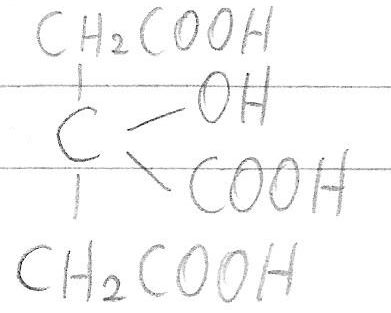
\includegraphics[scale=1]{citricAcid}
	\caption{\textgreek{Χημική εξίσωση Κιτρικού οξέως}}
	\label{fig:citricAcid}
	\end{figure}
	
	\textbullet \quad $\displaystyle CaCO_3$  :  \textgreek{Ανθρακικό ασβέστιο / ασβεστόλιθος / μάρμαρο} \linebreak 
	\textbullet \quad $\displaystyle CH_4N_2O$  :  \textgreek{Ουρία} \linebreak 
	\textbullet \quad $\displaystyle C_2H_4O_2 \ (CH_3COOH) $  :  \textgreek{Αιθανικό / οξικό οξύ} \linebreak 
	\textbullet \quad $\displaystyle C_9H_8O_4$  :  \textgreek{Ακετυλοσαλικιλικό οξύ / ασπιρίνη} \linebreak 
	\textbullet \quad $\displaystyle CHCl_3$  :  \textgreek{Τριχλωρομεθάνιο / Χλωροφόρμιο} \linebreak 
	\textbullet \quad $\displaystyle CaC_2$  :  \textgreek{Ανθρακασβέστιο} \linebreak 
	\textbullet \quad $\displaystyle Ca(OH)_2$  :  \textgreek{Ασβεστόνερο} \linebreak 
	\textbullet \quad $\displaystyle HCHO$  :  \textgreek{Μεθανάλη / Φορμαλδεύδη} \linebreak 
	\textbullet \quad \textgreek{2-υδροξυπροπανικό οξύ / Γαλακτικό οξύ} (\figref{lacticAcid}) \linebreak 
	
	\begin{figure}[H]
	\centering
	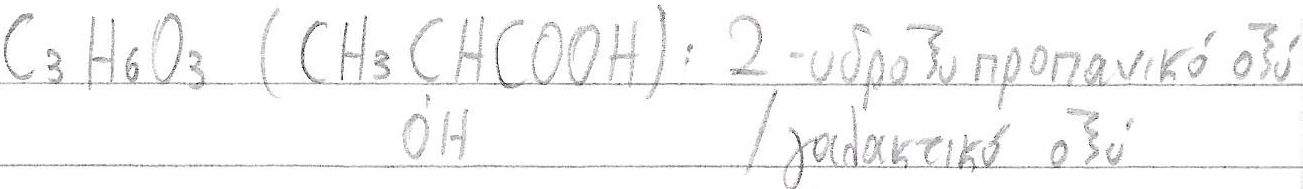
\includegraphics[scale=1]{lacticAcid}
	\caption{\textgreek{Χημική εξίσωση Γαλακτικού οξέως}}
	\label{fig:lacticAcid}
	\end{figure}
	
	\textbullet \quad $\displaystyle C_6H_5COOH $  :  \textgreek{Βενζοικό οξύ} / E120(\textgreek{συντηρητικό τροφίμων} \linebreak 
	
	\begin{figure}[H]
	\centering
	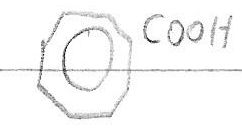
\includegraphics[scale=1.4]{cooh}
	\caption{\textgreek{Χημικός τύπος Καρβοξυλικού οξέος - } COOH - \textgreek{Βενζοικός δακτύλιος}}
	\label{fig:cooh}
	\end{figure}
	
	\textbullet \quad $\displaystyle C_4H_6O_6$  :  \textgreek{Χημικός τύπος Τρυγικού οξέως (απαντάται στο κρασί \& σε αναψυκτικά)} (\figref{tartaricAcid}) \linebreak 
	
	\begin{figure}[H]
	\centering
	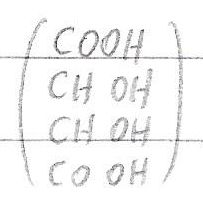
\includegraphics[scale=1.4]{tartaricAcid}
	\caption{\textgreek{Τρυγικό οξύ - Κρασί}}
	\label{fig:tartaricAcid}
	\end{figure}
	
	\textbullet \quad $\displaystyle CH_2O_2 / HCOOH $  :  \textgreek{Μεθανικό οξύ / Μυρμηκικό οξύ} \linebreak 
	\textbullet \quad $\displaystyle C_4H_8O_2 $  :  \textgreek{Βουτανικό / Βουτυρικό οξύ} \linebreak 
	\textbullet \quad \textgreek{Πυροσταφιλικό οξύ} (\figref{pirostafilikoOxi}) \linebreak 
	
	\begin{figure}[H]
	\centering
	\includegraphics[scale=1.4]{pirostafilikoOxi}
	\caption{\textgreek{Τρυγικό οξύ - Κρασί}}
	\label{fig:pirostafilikoOxi}
	\end{figure}
	
	
	\pagebreak
	
	
	\section{Economics}
	
	\textbullet \quad $\displaystyle a_{\nu} = a (1+ \tau)^{\nu}$  :  \textgreek{Τύπος του ανατοκισμού} \qquad \small{\textgreek{Αν καταθέσει κάποιος στη τράπεζα μετρητά, μετά από ν χρόνια θα εισπράξει}} $a_{\nu}$ \small{\textgreek{μετρητά}} \linebreak 
	\textgreek{α: κεφάλαιο}, $\displaystyle \tau = \frac{\epsilon(\%)}{100}$  :  \textgreek{τόκος τους ενός ευρώ σε 1 χρόνο} \linebreak 
	\textgreek{ν: χρόνια, ε: επιτόκιο $(\%)$} \linebreak 
	\textbullet \quad $\displaystyle \tau = \frac{\epsilon}{100} \cdot \alpha $  :  \textgreek{τόκος τ που αποδίδει το κεφάλαιο α με επιτόκιο ε} \linebreak 
	\textbullet \quad $\displaystyle \Sigma = \alpha (1+ \tau)\frac{(1+\tau)^{\nu}-1}{\tau} $  :  \textgreek{τύπος των ίσων καταθέσεων} \linebreak 
	\textbullet \quad \textgreek{Κόστος ευκαιρίας του αγαθού} $\displaystyle Y = \frac{\text{\textgreek{Μονάδες του αγαθού Χ που θυσιάζονται}}}{\text{\textgreek{Μονάδες του αγαθού Υ που παράγονται}}} $ \qquad \textgreek{σε όρους του αγαθού Χ} \linebreak 
	\textgreek{ή} $\displaystyle KE_y = \frac{\Delta X}{\Delta Y}$  :  \textgreek{οι μονάδες του αγαθού Χ που θυσιάστηκαν για την παραγωγή μιας επιπλέον μονάδας του Υ} \linebreak 
	\textbullet \quad $\displaystyle E_D = \frac{\Delta Q}{\Delta P} \cdot \frac{P_1}{Q_1} $  :  \textgreek{Ελαστικότητα της ζήτησης στο σημείο που αντιστοιχεί σε τιμή} $P_1$ \textgreek{και ζητούμενη ποσότητα} $Q_1$. \linebreak 
	$\displaystyle |E_D| > 1 \rightarrow \left| \frac{\Delta Q}{Q} \right| > \left| \frac{\Delta P}{P} \right| $  :  \textgreek{Ελαστική ζήτηση} \linebreak 
	$\displaystyle |E_D| < 1 \rightarrow \left| \frac{\Delta Q}{Q} \right| < \left| \frac{\Delta P}{P} \right| $  :  \textgreek{Ανελαστική ζήτηση} \linebreak 
	\textbullet \quad $\displaystyle \text{\textgreek{Μέσο προιόν}}(AP) = \frac{\text{\textgreek{Συνολικό προιόν}}(Q)}{\text{\textgreek{Ποσότητα μεταβλητού συντελεστή}}} $ \linebreak 
	\textbullet \quad $\displaystyle \text{\textgreek{Οριακό προιόν}}(MP) = \frac{\text{\textgreek{Μεταβολή συνολικού προιόντος}}(\Delta Q)}{\text{\textgreek{Μεταβολή ποσότητας μεταβλητού συντελεστής}}}$ \linebreak 
	\textbullet \quad $\displaystyle \text{\textgreek{Μέσο σταθερό κόστος}}(AFC) = \frac{\text{\textgreek{Σταθ. Κόστος}}(FC)}{\text{\textgreek{Ποσότητα παραγωγής}}(Q)} $ \linebreak 

	\textbullet \quad $\displaystyle \text{\textgreek{Μέσο μεταβλητό κόστος}}(AVC) = \frac{\text{\textgreek{Μεταβλητό κόστος}}(VC)}{\text{\textgreek{Ποσότητα παραγωγής}}(Q)}$ \linebreak 
	\textbullet \quad $ \text{\textgreek{Μέσο συνολικό κόστος}}(ATC) = \frac{\text{\textgreek{Συνολικό κόστος}}(TC)}{\text{\textgreek{Ποσότητα παραγωγής}}(Q)} $ \linebreak 
	\textbullet \quad $ ATC = AFC + AVC$ \linebreak 
	\textbullet \quad $\displaystyle \text{\textgreek{Οριακό κόστος}}(MC) = \frac{\text{\textgreek{Μεταβολή συνολικού κόστους}}[\Delta (TC)]}{\text{\textgreek{Μεταβολή του προιόντος}}[\Delta Q]} = \frac{\text{\textgreek{Μεταβολή μεταβλητού κόστους}}[\Delta CVC]}{\text{\textgreek{Μεταβολή του προιόντος}}[\Delta Q]} $ \linebreak 
	\textgreek{Δείχνει το ρυθμό με τον οποίο μεταβάλλεται το συνολικό κόστος, όταν μεταβάλλεται η παραγωγή κατά μια μονάδα}
	\textbullet \quad \textgreek{Οι παραπάνω 5 τύποι αφορούν τη βραχυχρόνια περίοδο. Κατά τη μακροχρόνια περίοδο όλοι οι παραγωγικοί συντελεστές δύναται να μεταβληθούν} \linebreak 
	\textbullet \quad $\displaystyle E_s = \frac{\Delta Q}{\Delta P} \cdot \frac{P_1}{Q_1} $  :  \textgreek{Ελαστικότητα της προσφοράς, όπου}: $\Delta Q$  :  \textgreek{μεταβολή προσφερόμενης ποσότητας}, $\Delta P$  :  \textgreek{μεταβολή τιμής}, $P_1$  :  \textgreek{αρχική τιμή}, $Q_1$  :  \textgreek{αρχική ποσότητα} \linebreak 
	\textbullet \quad \textgreek{Συνάρτηση ζήτησης}: $Q_D = f(P)$ \textgreek{έχει αρνητική κλίση (η καμπύλη} $D$). \textgreek{Συνάρτηση προσφοράς} $Q_s = f(P)$ \textgreek{έχει θετική κλίση (η καμπύλη} $S$). \linebreak 
	\textbullet \quad Total Revenue $(TR) = P\cdot Q$  :  \textgreek{Συνολικά έσοδα (επιχείρησης)} \linebreak 
	$P$  :  \textgreek{τιμή}, $Q$  :  \textgreek{πωλούμενη ποσότητα} \linebreak 
	\textbullet \quad Average Revenue $\displaystyle (AR) = \frac{RT}{Q} $  :  \textgreek{Μέσο έσοδο} \linebreak 
	\textbullet \quad Marginal Revenue $\displaystyle (MR) = \frac{\Delta (P\cdot Q)}{\Delta Q} $  :  \textgreek{Επιπλέον έσοδο από την πώληδη μιας επιπλέον ποσότητας προιόντος} \linebreak 
	\textbullet \quad $\displaystyle K = TR - TC = (AR - ATC) \cdot Q $  :  \textgreek{Κέρδος (ή ζημία)} \linebreak 
	\textbullet \quad \textgreek{Καθαρή επένδυση = Ακαθάριστη ιδιωτική επένδυση - Αποσβέσεις} \linebreak 
	\textbullet \quad \textgreek{Α.Ε.Π. = Ιδιώτικη κατανάλωση + Ακαθάριστη ιδιωτική επένδυση + Κρατική ή Δημόσια δαπάνη + (Εξαγωγές - Εισαγωγές)} \linebreak 
	\textbullet \quad \textgreek{Εξαγωγές - Εισαγωγές = Καθαρό εισόδημα από το εξωτερικό} \linebreak 
	\textbullet \quad \textgreek{Α.Ε.Π. = Μισθοί + Πρόσοδοι περιουσίας + Τόκοι + Κέρδη + Αποσβέσεις + Έμμεσοι φόροι - Κρατικές επιδοτήσεις - Τόκοι Δημοσίου χρέους - Καθαρό εισόδημα από το εξωτερικό} \linebreak 
	\textbullet \quad \textgreek{Α.Ε.Θ.Π. = Α.Ε.Π. + Καθαρό εισόδημα από το εξωτερικό} \linebreak 
	\textbullet \quad \textgreek{Κ.Ε.Θ.Π. = Α.Ε.Θ.Π. - Αποσβέσεις} \linebreak 
	\textbullet \quad \textgreek{Καθαροί έμμεσοι φόροι = Έμμεσοι φόροι - Επιδοτήσεις} \linebreak 
	\textbullet \quad \textgreek{Εθνικό εισόδημα = Κ.Ε.Θ.Π. - Καθαροί έμμεσοι φόροι} \linebreak 
	\textbullet \quad \textgreek{Διαθέσιμο εισόδημα = Εθνικό εισόδημα + Μεταβιβαστικές πληρωμές + Τόκοι του δημόσιου χρέους - Αδιανέμητα κέρδη - Άμεσοι φόροι} \linebreak 
	\textbullet \quad \textgreek{Αποταμίευση = Διαθέσιμο εισόδημα - Κατανάλωση} \linebreak 
	\textbullet \quad \textgreek{Κατά κεφαλήν πραγματικό Α.Ε.Π. =} $\displaystyle \frac{\text{\textgreek{Πραγματικό Α.Ε.Π.}}}{\text{\textgreek{Πληθυσμός}}} $ \linebreak 
	\textbullet \quad \textgreek{Ποσοστό ρευστών διαθεσίμων = Ποσοστό χρημάτων που η τράπεζα διατηρεί αποθηκευμένο στα ταμεία της για κάθε 100 ευρώ φυσικού συναλλάγματος που διαθέτει} \linebreak 
	\textbullet \quad \textgreek{Πραγματικό εισόδημα = } $\displaystyle \frac{\text{\textgreek{Ονομαστικό Εισόδημα}}}{\text{\textgreek{Επίπεδο τιμών}}} \cdot 100 \ (\%) $ \linebreak 
	\textbullet \quad \textgreek{Ποσοστό ανεργίας = } $\displaystyle \frac{\text{\textgreek{Αριθμός ανέργων}}}{\text{\textgreek{Εργατικό δυναμικό}}} \cdot 100 \ (\%) $ \linebreak 
		
			
\end{flushleft}

\end{document}